\documentclass[11pt,twoside,openright]{book}
%%%%%%%%%%%%%%%%%%%%%%%%% PACKAGES %%%%%%%%%%%%%%%%%%%%%%%%%%
\usepackage[utf8]{inputenc}
\usepackage{textcomp}
\usepackage[english]{babel}
\usepackage{graphicx}
\usepackage{bm}
\usepackage{url}
\usepackage{rotating}
\usepackage{amsfonts}
\usepackage{verbatim}
\usepackage{amssymb}
\usepackage{pifont}
\usepackage{amsthm}
\usepackage{graphicx}
\usepackage{algorithmic}
\usepackage{algorithm}
\usepackage{listings}
\usepackage{cite}
\usepackage{fix2col}
\usepackage{color}
\usepackage{geometry}
\usepackage{longtable}
\usepackage{chngpage}
\usepackage{amsmath}
\usepackage{booktabs}
\usepackage{subfig}
\usepackage{pifont}
\usepackage{multirow}
\usepackage{lscape}
\usepackage{xspace}
\usepackage{mdwtab}
\usepackage{float}
%\usepackage{mathptmx}        % selects Times Roman as basic font
\usepackage{helvet}          % selects Helvetica as sans-serif font
\usepackage{courier}         % selects Courier as typewriter font
\usepackage{type1cm}         % activate if the above 3 fonts are not available on your system
\usepackage{makeidx}         % allows index generation
\usepackage{graphicx}        % standard LaTeX graphics tool when including figure files
\usepackage{multicol}        % used for the two-column index
\usepackage[bottom]{footmisc}% places footnotes at page bottom
%\usepackage[hidelinks, breaklinks]{hyperref}
%\usepackage{epsfig}
\usepackage{amssymb}
\usepackage{array}
\usepackage{tikz}
\usepackage{pdfpages}
% \usepackage{algorithm}
%\usepackage{algorithmic}
% \usepackage{algorithmicx}
% \usepackage{algpseudocode}
% \algdef{SE}[DOWHILE]{Do}{doWhile}{\algorithmicdo}[1]{\algorithmicwhile\ #1}%

\usepackage[pdftex,
            pdfauthor={Christophe Rigaud},
            pdftitle={Segmentation and indexation of complex objects in comic book images},
            pdfsubject={PhD thesis of Christophe Rigaud},
            pdfkeywords={image processing, document analysis, graphic recognition, comics understanding},
            pdfproducer={Latex with hyperref, or other system},
            pdfcreator={pdflatex, or other tool}]{hyperref}                 % Active hyperlink
            
\usepackage[hyperpageref]{backref}    % Add 'backlink' page number at the end of each item in the bibliography BibTeX
\hypersetup{
    %Since 2011-02-05 (hyperref version 6.82a), you can use the hidelinks option to achieve the same result
    colorlinks=false,
    pdfborder={0 0 0},
}

% XML script listing
\definecolor{gray}{rgb}{0.4,0.4,0.4}
\lstset{
  basicstyle=\footnotesize\ttfamily,
  columns=fullflexible,
  showstringspaces=false,
  breaklines=true,
  commentstyle=\color{gray}\upshape
}

\lstdefinelanguage{XML}
{
  morestring=[b]",
  morestring=[s]{>}{<},
  morecomment=[s]{<?}{?>},
  stringstyle=\color{black},
  identifierstyle=\color{blue},
  keywordstyle=\color{red},
  morekeywords={confidence, class, points, id, label, x, y, width, height, href, collectionTitle, editorName, doublePage, website, albumTitle, drawerName, language, resolution, ISBN, readingDirection, writerName, releaseDate, pageNumber, rank}% list your attributes here
}


%\usetikzlibrary{fit,arrows,matrix,calc,positioning,shapes,backgrounds}
%\usepackage{algpseudocode}
%%%%%%%%%%%%%%%%%%%%%%%%% INCLUDES %%%%%%%%%%%%%%%%%%%%%%%%%%
%\newcommand{\RR}{\rm I\hspace{-0.55ex}R}
%\newcommand{\NN}{\rm I\hspace{-0.55ex}N}
%\renewcommand{\baselinestretch}{1.0}

% New theorems
\theoremstyle{definition}
\newtheorem{definition}{Definition}[chapter]
\newtheorem{theorem}{Theorem}[section]

\theoremstyle{plain}
\newtheorem{lemma}[theorem]{Lemma}
\newtheorem{proposition}[theorem]{Proposition}
\newtheorem{corollary}[theorem]{Corollary}

% Own commands
\newcommand{\ie}{{\em i.e.~}}
\newcommand{\mI}{\mathbf{I}}
\newcommand{\mone}{\mathbf{1}}
\newcommand{\eg}{{\em e.g.~}}
\newcommand{\etal}{{\em et al.}}
\newcommand{\vs}{{\em vs}}
\newcommand{\fig}[1]{Figure \ref{#1}}
\newcommand{\eq}[1]{Eqn. \ref{#1}}
\newcommand{\sect}[1]{Section \ref{#1}}
\newcommand{\ch}[1]{Chapter \ref{#1}}
\newcommand{\app}[1]{Appendix \ref{#1}}
\newcommand{\dataset}{{\cal D}}
\newcommand{\fracpartial}[2]{\frac{\partial #1}{\partial  #2}}
\newcommand{\mycaption}[1]{\caption{ \protect{{\small\sf #1}} }}
\newcommand{\mcomma}{, \allowbreak}
\newcommand{\cmark}{\ding{51}}
\newcommand{\xmark}{\ding{55}}

% Own Operators
\DeclareMathOperator*{\argmax}{arg\,max}


% PAMI
\newcommand{\D}{\delta}
\newcommand{\fspc}{\Omega}
\newcommand{\lspc}{\mathcal{Y}}
\newcommand{\sspc}{\mathcal{S}}

\newcommand{\desc}{\mathbf{D}}
\newcommand{\oracle}{{\mathcal{O}}}
\newcommand{\vx}{\mathbf{x}}
\newcommand{\sample}{\mathbf{s}}
\newcommand{\lab}{y}

\newcommand{\ActPos}{Act$+$}
\newcommand{\ActNeg}{Act$-$}
\newcommand{\ActPosNeg}{Act$\pm$}
\newcommand{\ActGT}{Act$\sim$}

\newcommand{\pD}{p(\sample,\lab)}
\newcommand{\pDvx}{p(\vx,\lab)}

\newcommand{\training}{tr}
\newcommand{\testing}{tt}

\newcommand{\vxTr}{\vx^{\training}}
\newcommand{\sampleTr}{\sample^{\training}}
\newcommand{\labTr}{\lab^{\training}}

\newcommand{\vxTt}{\vx^{\testing}}
\newcommand{\sampleTt}{\sample^{\testing}}
\newcommand{\labTt}{\lab^{\testing}}

\newcommand{\TS}{\mathcal{T}}
\newcommand{\TrS}{\TS^{\training}}
\newcommand{\TrSPos}{\TS^{\training +}}
\newcommand{\TrSNeg}{\TS^{\training -}}
\newcommand{\TtS}{\TS^{\testing}}

\newcommand{\clsf}{\mathrm{C}}
\newcommand{\detect}{\mathrm{D}}

\newcommand{\Ds}{\D_s}
\newcommand{\Dt}{\D_t}
\newcommand{\pDs}{p_{s}(\sample,\lab)}
\newcommand{\pDt}{p_{t}(\sample,\lab)}
\newcommand{\pDvxs}{p_{s}(\vx,\lab)}
\newcommand{\pDvxt}{p_{t}(\vx,\lab)}
\newcommand{\TrSs}{\TS^{\training, s}}
\newcommand{\TrSt}{\TS^{\training, t}}
\newcommand{\TrSPoss}{\TS^{\training +, s}}
\newcommand{\TrSPost}{\TS^{\training +, t}}
\newcommand{\TtSt}{\TS^{\testing, t}}

\newcommand{\Daimler}{{\mathcal{D}}}
\newcommand{\INRIA}{{\mathcal{I}}}
\newcommand{\Virtual}{{\mathcal{V}}}

\newcommand{\SX}{\mathcal{X}}
\newcommand{\SR}{\mathcal{R}}
\newcommand{\TrSX}{\TrS_{\SX}}
\newcommand{\TrSR}{\TrS_{\SR}}
\newcommand{\TtSR}{\TtS_{\SR}}

\newcommand{\TrSVirtual}{\TrS_{\Virtual}}
\newcommand{\TrSINRIA}{\TrS_{\INRIA}}
\newcommand{\TrSDaimler}{\TrS_{\Daimler}}
\newcommand{\TtSINRIA}{\TtS_{\mathcal{I}}}
\newcommand{\TtSDaimler}{\TtS_{\Daimler}}

\newcommand{\TrSVirtualPos}{\TrSPos_{\Virtual}}
\newcommand{\TrSINRIAPos}{\TrSPos_{\INRIA}}
\newcommand{\TrSDaimlerPos}{\TrSPos_{\Daimler}}
\newcommand{\TrSXPos}{\TrSPos_{\SX}}
\newcommand{\TrSRPos}{\TrSPos_{\SR}}

\newcommand{\TrSVirtualNeg}{\TrSNeg_{\Virtual}}
\newcommand{\TrSINRIANeg}{\TrSNeg_{\INRIA}}
\newcommand{\TrSDaimlerNeg}{\TrSNeg_{\Daimler}}
\newcommand{\TrSXNeg}{\TrSNeg_{\SX}}
\newcommand{\TrSRNeg}{\TrSNeg_{\SR}}

\newcommand{\TrTt}[2]{\{#1,#2\}}

\newcommand{\Source}{\Virtual}
\newcommand{\Target}{\SR}

\newcommand{\TrSTarget}{\TrS_{\Target}}
\newcommand{\TtSTarget}{\TtS_{\Target}}

\newcommand{\ImSet}{\Im}
\newcommand{\TrIS}{\ImSet^{\training}}
\newcommand{\TrISPos}{\ImSet^{\training +}}
\newcommand{\TrISNeg}{\ImSet^{\training -}}
\newcommand{\TtIS}{\ImSet^{\testing}}

\newcommand{\TrISSourcePos}{\TrISPos_{\Virtual}}
\newcommand{\TrISSourceNeg}{\TrISNeg_{\Virtual}}
\newcommand{\TrISSource}{\TrIS_{\Virtual}}

\newcommand{\TrISTargetPos}{\TrISPos_{\Target}}
\newcommand{\TrISTargetNeg}{\TrISNeg_{\Target}}
\newcommand{\TrISTarget}{\TrIS_{\Target}}

%\newcommand{\TtISTarget}{\TtIS_{\Target}}

\newcommand{\TrSSourcePos}{\TrSVirtualPos}
\newcommand{\TrSSourceNeg}{\TrSVirtualNeg}

\newcommand{\TrSTargetPos}{\TrSPos_{\Target}}
\newcommand{\TrSTargetNeg}{\TrSNeg_{\Target}}

\newcommand{\TrISVirtualPos}{\TrISSourcePos}
\newcommand{\TrISVirtualNeg}{\TrISSourceNeg}

\newcommand{\TrISINRIAPos}{\TrISPos_{\INRIA}}
\newcommand{\TrISINRIANeg}{\TrISNeg_{\INRIA}}

\newcommand{\TrISDaimlerPos}{\TrISPos_{\Daimler}}
\newcommand{\TrISDaimlerNeg}{\TrISNeg_{\Daimler}}

\newcommand{\TrISXPos}{\TrISPos_{\SX}}
\newcommand{\TrISXNeg}{\TrISNeg_{\SX}}
\newcommand{\TrISRPos}{\TrISPos_{\SR}}
\newcommand{\TrISRNeg}{\TrISNeg_{\SR}}


\newcommand{\AMR}{AMR}

\usepackage{color}
\definecolor{red}{rgb}{1.00,0.20,0.20}
\definecolor{blue}{rgb}{0.20,0.20,1.00}
\definecolor{green}{rgb}{0.00,1.00,0.00}
\newcommand{\cred}[1] {\textcolor{red}{#1}} % To revise (shorten in some cases).
\newcommand{\cblue}[1] {\textcolor{blue}{#1}}
\newcommand{\cgreen}[1] {\textcolor{green}{#1}}  % Comments

%% Consolider
\newcommand{\VTrain}{\mathcal{V}^{\mbox{{\tiny train}}}}
\newcommand{\VTrainP}{\mathcal{V}_+^{\mbox{{\tiny train}}}}
\newcommand{\VTrainN}{\mathcal{V}_-^{\mbox{{\tiny train}}}}

\newcommand{\ITest}{\mathcal{I}^{\mbox{{\tiny test}}}}
\newcommand{\ITestPi}{\mathcal{I}_+^{\mbox{{\tiny i,test}}}}
\newcommand{\ITestNi}{\mathcal{I}_-^{\mbox{{\tiny i,test}}}}

\newcommand{\ITrain}{\mathcal{I}^{\mbox{{\tiny train}}}}
\newcommand{\ITrainP}{\mathcal{I}_+^{\mbox{{\tiny train}}}}
\newcommand{\ITrainN}{\mathcal{I}_-^{\mbox{{\tiny train}}}}
\newcommand{\ITrainNi}{\mathcal{I}_-^{\mbox{{\tiny i,train}}}}

\newcommand{\VCP}{\mathcal{C}_\mathcal{V}^{\mbox{{\tiny pas}}}}
\newcommand{\VCA}{\mathcal{C}_\mathcal{V}^{\mbox{{\tiny act}}}}
\newcommand{\ICP}{\mathcal{C}_\mathcal{I}^{\mbox{{\tiny pas}}}}

\newcommand{\classifier}{\mathcal{C}}
\newcommand{\st}{x_t}
\newcommand{\class}{w_t}

%% ICPR
\newcommand{\Real}{\mathcal{R}}
\newcommand{\posLabel}{+}
\newcommand{\negLabel}{-}
\newcommand{\unlabel}{?}
\newcommand{\TrISCVC}{\ImSet^{\training}_{cvc}}
\newcommand{\TrSDet}{\TS^{\training \unlabel}}
\newcommand{\TrSTargetDet}{\TrSDet_{\Target}}

%% CVPR workshop
\newcommand{\learner}{\mathcal{L}}



%%%%%%%%%%%%%%%%%%%%%%%%%%%%%%%%%%%%%%%%%%%%%

\makeatletter
\newlength \fullwidth
  \setlength \fullwidth {\columnwidth}
\makeatother

\makeatletter
\newlength \figwidth
  \setlength \figwidth {1.00\columnwidth}
\makeatother

\makeatletter
\newlength \plotwidth
  \setlength \plotwidth {0.75\columnwidth}
\makeatother

\makeatletter
\newlength \plotwidthTwo
  \setlength \plotwidthTwo {0.50\columnwidth}
\makeatother

\makeatletter
\newlength \plotwidthThree
  \setlength \plotwidthThree {0.33\columnwidth}
\makeatother


% Conferences and Journal Abbreviations
\newcommand{\TPAMI}{IEEE Trans. on Pattern Analysis and Machine Intelligence}
\newcommand{\TVT}{IEEE Trans. on Vehicular Technology}
\newcommand{\TNN}{IEEE Trans. on Neural Networks}
\newcommand{\TITS}{IEEE Trans. on Intelligent Transportation Systems}
\newcommand{\TIP}{IEEE Trans. on Image Processing}
\newcommand{\IS}{IEEE Intelligent Systems}
\newcommand{\Spectrum}{IEEE Spectrum}
\newcommand{\ProcIEEE}{Proceedings of the IEEE}
\newcommand{\PRL}{Pattern Recognition Letters}
\newcommand{\PR}{Pattern Recognition}
\newcommand{\IJCV}{Int. Journal on Computer Vision}
\newcommand{\IVC}{Image and Vision Computing}
\newcommand{\CVIU}{Computer Vision and Image Understanding}
\newcommand{\ML}{Machine Learning}
\newcommand{\JAIR}{Journal of Artificial Intelligence Research}
\newcommand{\JMLR}{Journal of Machine Learning Research}
\newcommand{\JCSS}{Journal of Computer and System Sciences}
\newcommand{\CYBER}{IEEE Trans. on Systems, Man, and Cybernetics (Part B)}
\newcommand{\SPI}{Journal of statistical planning and inference}
\newcommand{\KDE}{IEEE Trans. on Knowledge and Data Engineering}


\newcommand{\CVPR}{IEEE Conf. on Computer Vision and Pattern Recognition}
\newcommand{\IV}{IEEE Intelligent Vehicles Symposium}
\newcommand{\ITSC}{IEEE Int. Conf. on Intelligent Transportation Systems}
\newcommand{\ICIG}{IEEE Int. Conf. on Image and Graphics}
\newcommand{\SISPA}{IEEE Int. Symp. on Image and Signal Processing and Analysis}
\newcommand{\IRTA}{SPIE Conf. Infrared Technology and Applications}
\newcommand{\ICRA}{IEEE Int. Conf. on Robotics and Automation}
\newcommand{\VTC}{IEEE Vehicular Technology Conference}
\newcommand{\ICPR}{Int. Conf. in Pattern Recognition}
\newcommand{\ICCV}{Int. Conf. on Computer Vision}
\newcommand{\ECCV}{European Conf. on Computer Vision}
\newcommand{\ICIP}{IEEE Int. Conf. on Image Processing}
\newcommand{\ACIVS}{Advanced Concepts for Intelligent Vision Systems}
\newcommand{\ICDE}{IEEE Int. Conf. on Data Engineering Workshop}
\newcommand{\BMVC}{British Machine Vision Conference}
\newcommand{\DAGM}{German Association for Pattern Recognition (DAGM) Conference}
\newcommand{\NIPS}{Advances in Neural Information Processing Systems}
\newcommand{\ACMCHI}{ACM SIGCHI Conf. on Human Factors in Computing Systems}
\newcommand{\EUROGRAPHICS}{European Computer Graphics Conference and Exhibition}
\newcommand{\ACVHL}{Advancing Computer Vision with Humans in the Loop}
\newcommand{\CHI}{ACM Int. Conf. on Human Factors in Computing Systems}
\newcommand{\APGV}{Symposium on Applied Perception in Graphics and Visualization}
\newcommand{\VIIP}{IASTED Int. Conference on Visualization, Imaging and Image Processing}
\newcommand{\ICCVS}{Int. Conf. on Computer Vision Systems}
\newcommand{\ACL}{Meeting of the Association for Computational Linguistics}
\newcommand{\COLT}{Conference on Learning Theory}
\newcommand{\ACCV}{Asian Conf. on Computer Vision}
\newcommand{\VSPETS}{Joint IEEE Int. Works. on Visual Surveillance and Performance Evalutation of Tracking and Surveillance}
\newcommand{\SIGGRAPHASIA}{ACM SIGGRAPH Conf. and Exhib. on Computer Graphics and Interactive Techniques in Asia}
\newcommand{\ICMI}{ACM International Conference on Multimodal Interaction}
\newcommand{\ICVS}{International Conference on Computer Vision Systems}
\newcommand{\NIPSWDA}{Advances in Neural Information Processing Systems. Domain Adaptation Workshop: Theory and Application}
\newcommand{\CAIP}{Int. Conf. on Computer Analysis of Images and Patterns}
\newcommand{\ICML}{Int. Conf. on Machine Learning}
\newcommand{\IBPRIA}{Iberian Conf. on Pattern Recognition and Image Analysis}
\newcommand{\CVPRGT}{IEEE Conf. on Computer Vision and Pattern Recognition. Ground Truth Workshop: What is a good dataset?} 
\newcommand{\EMNLP}{Int. Conf. on Empirical Methods in Natural Language Processing} 
\newcommand{\PPKDD}{European Conf. on Principles and Practice of Knowledge Discovery in Databases} 
\newcommand{\AMACL}{Annual Meeting of the Association for Computational Linguistics} 
\newcommand{\IDA}{Intelligent Data Analysis} 

%Very special characters
%\DeclareInputText{39}{'}
\DeclareGraphicsExtensions{.pdf,.png}
\graphicspath{{./figs/}}

%%%%%%%%%%%%%%%%%%%%%%%%% TITLE, AUTHOR, DIRECTORS %%%%%%%%%%%%%%%%%%%%%%%%%%
%\title{Segmentation and indexation of graphical objects: application to detection and recognition of complex object from comic books}
%\title{Understanding of comic images from pixel to semantics}
\title{Segmentation and indexation of complex objects in comic book images}
\author{\href{http://www.christophe-rigaud.com}{Christophe Rigaud}}
\date{September 29, 2014}
 

\newcommand{\UAB}{Universitat Aut\`{o}noma de Barcelona}
\newcommand{\ULR}{Université de La Rochelle}
\newcommand{\CVC}{Centre de Visió per Computador}
\newcommand{\LIII}{Laboratoire Informatique, Image et Interaction}
\newcommand{\DCC}{Dept. Ciències de la Computació}
\newcommand{\DCCCVC}{\DCC{} \& \CVC{}}
\newcommand{\CVPRU}{Computer Vision and Pattern Recognition Unit}
\newcommand{\ISI}{Indian Statistical Institute}
\newcommand{\CVPRUISI}{\CVPRU{} \& \ISI{}}

\newcommand{\printer}{Ediciones Gráficas Rey, S.L.}
\newcommand{\dedication}{To my parents...}
\newcommand{\sentence}{\textit{Nothing in life is to be feared,}\\ \textit{it is only to be understood.}\\Maria Skłodowska-Curie (1867 - 1934)\\ \vspace{1cm}\textit{Live as if you were to die tomorrow.}\\ \textit{Learn as if you were to live forever}\\Mahatma Gandhi (1869 - 1948)}

\newcommand{\ISBN}{}
%%%%%%%%%%%%%%%%%%%%%%%%% DEFINICIONS DEL ESTIL CVC %%%%%%%%%%%%%%%%%%%%%%%%%%
\setlength{\paperheight   }{240mm}
\setlength{\paperwidth    }{170mm}
\setlength{\hoffset       }{  0pt}
\setlength{\voffset       }{  0pt}
\setlength{\textwidth     }{130mm}
\setlength{\textheight    }{195mm}
\setlength{\headsep       }{  9mm}
\setlength{\topmargin     }{-37pt}
\setlength{\oddsidemargin }{  0cm}
\setlength{\evensidemargin}{  0pt}
\addtolength{\evensidemargin}{-2in}
\addtolength{\evensidemargin}{+4cm}
%\addtolength{\evensidemargin}{0mm}   % retocar para que las dos caras casen

\newlength{\reducedwidth}
\setlength{\reducedwidth}{\textwidth}
\addtolength{\reducedwidth}{-\parindent}
\addtolength{\reducedwidth}{-\parindent}
\renewcommand{\chaptermark}[1]{\markboth{\MakeUppercase{#1}}{}}
\renewcommand{\sectionmark}[1]{\markright{\thesection.\ #1}}

%\makeatletter
%\def\chapter{\clearpage\thispagestyle{plain}\global\@topnum
%   \z@\@afterindentfalse
%   \secdef\@chapter\@schapter
%}
%\makeatother
%\title{My Picture Chapters}
%\begin{document}
%\maketitle

%Modifications in red
\newcommand{\modif}[1]{{\bf\color{red}#1}}
\newcommand{\concept}[1]{{\it#1}}
\newcommand{\objProp}[1]{{\it#1}}
\newcommand{\dataProp}[1]{{\it#1}}

\newcommand{\blankpage}{
\newpage
\thispagestyle{empty}
\mbox{}
\newpage
}

\newcommand{\chapterwithpic}[4][]{
  \blankpage
  \clearpage\thispagestyle{empty}
  \begin{figure}[t!]
    \begin{center}
      \includegraphics[width=0.75\figwidth]{#3}\\
      #4
    \end{center}    
    %\caption[#4]{#4}
  \end{figure}  
  \chapter[#1]{#2}
}

\makeatletter
\long\def\@makecaption#1#2{%
   \vskip 10\p@
   \small
   \setbox\@tempboxa\hbox{\textbf{#1:} #2}%
   \ifdim \wd\@tempboxa >\reducedwidth
    \hfil\parbox{\reducedwidth}{\textbf{#1:} #2}\hfil
     \else
       \hbox to\hsize{\hfil\box\@tempboxa\hfil}%
   \fi}

\def\@makechapterhead#1{%
  \vspace*{50\p@}%
  {\parindent \z@ \raggedright \normalfont
    \ifnum \c@secnumdepth >\m@ne
      \if@mainmatter
        \Huge \bfseries \@chapapp\space \thechapter
        \par\nobreak
        \vskip 20\p@
      \fi
    \fi
    \interlinepenalty\@M
    \huge \bfseries #1\par\nobreak
    \vskip 40\p@
  }}

\newcommand{\makefirstpages}{
  \thispagestyle{empty}
  \vspace*{0.5cm}
  \begin{center}
\includegraphics[width=6cm]{images/LogoUAB}\end{center}
  \vspace*{3cm}
  \parbox{\textwidth}{\addtolength{\lineskip}{5pt} \centering \textbf{\LARGE \@title}  }
  \vfill0
  \begin{flushright}
  \parbox{7.5cm}{A dissertation submitted by \textbf{\@author} at \UAB{} to fulfil the degree of \textbf{Doctor of Philosophy}.\par
%  \vspace{2mm}
%  \parbox{7.5cm}{Director: \textbf{Dr. Josep Lladós Canet}.\\Departament: Ciències de la Computació, Escola d'Enginyeria, UAB.\\PhD Program: Informàtica.}\par
    \vspace*{2mm}
    \hfill Bellaterra, \@date
  }
  \end{flushright}

\blankpage

  %%%%%%%%%%%%%%%%%%%%%%%%%% NEW PAGE %%%%%%%%%%%%%%%%%%%%%%%%%%%%%%
  
\includepdf{template_ULR/frontpage.pdf}
  % \newpage

  %%%%%%%%%%%%%%%%%%%%%%%%%% NEW PAGE %%%%%%%%%%%%%%%%%%%%%%%%%%%%%%

  \clearpage
  \small
  \thispagestyle{empty}
  \noindent
  \begin{tabular}{>{\scriptsize}p{2cm}|>{\scriptsize}l}
  
   Director  & \textbf{Prof. Dr. Jean-Christophe Burie}\\
             & \LIII\\
             & \ULR~(France)\\

  \multicolumn{2}{c}{}\\
  
Co-Directors & \textbf{Dr. Dimosthenis Karatzas}\\
             & \CVC\\
             & \UAB~(Spain)\\
             & \\

             & \textbf{Prof. Dr. Jean-Marc Ogier}\\
             & \LIII\\
             & \ULR~(France)\\

  \multicolumn{2}{c}{}\\
             
                         
Thesis       & \textbf{Prof. Dr. Bart Lamiroy}\\
committee    & Laboratoire Lorrain de Recherche en Informatique et ses Applications\\
		         & Université de Lorraine (France)\\
             & \\     

             & \textbf{Prof. Dr. Koichi Kise}\\
             & Department of Computer Science and Intelligent Systems\\
             & Osaka Prefecture University (Japan)\\
             & \\
             
 
             & \textbf{Prof. Dr. Jean-Philippe Domenger}\\
             & Laboratoire Bordelais de Recherche en Informatique\\
		         & Université de Bordeaux (France)\\
             & \\

             & \textbf{Dr. Nicholas Journet}\\
             & Laboratoire Bordelais de Recherche en Informatique\\
             & Université de Bordeaux (France)\\

  \multicolumn{2}{c}{}\\
    
European     & \textbf{Dr. Simone Marinai}\\
evaluators   & Dipartimento di Ingegneria dell'Informazione\\
             & Università degli Studi di Firenze (Italy)\\
             & \\
                      
		         & \textbf{Dr. Apostolos Antonacopoulos}\\
			       & The School of Computing, Science \& Engineering\\
    	       & University of Salford (United Kingdom)\\
             
  \end{tabular}
  \vfill

  %%%%%%%%%%%%%%%%%%%%%%%%%% NEW PAGE %%%%%%%%%%%%%%%%%%%%%%%%%%%%%%

  \noindent
  \begin{minipage}{\textwidth}
  \setlength{\parskip}{10pt}
  \noindent \rule{60mm}{0.4mm} 
  
\includegraphics[trim=-5mm 5mm 0mm 0mm,width=2.8cm]{images/LogoL3i}
  
\includegraphics[trim=40mm 60mm 60mm 100mm,width=3.5cm]{images/LogoCVC}  \par
  \vspace*{0.5cm}
  \scriptsize{This document was typeset by the author using \LaTeXe.\par}
  \scriptsize{The research described in this book was carried out at the Laboratoire Informatique, Image et Interaction, Universtité de La Rochelle and at the \CVC, \UAB.\par}
  \scriptsize{Copyright $\copyright$ \number\year ~by \@author. All rights reserved. No part of this publication may be reproduced or transmitted in any form or by any means, electronic or mechanical, including photocopy, recording, or any information storage and retrieval system, without permission in writing from the author.\par}
  \scriptsize{ISBN: XXX \ISBN\par}
  \scriptsize{Printed by \printer}
  \end{minipage}
  \clearpage\thispagestyle{empty}
  \vspace*{6cm}
  \begin{flushright} \dedication \end{flushright}
  \clearpage\thispagestyle{empty}
    \vspace*{6cm}
  \begin{flushright} \sentence \end{flushright}
  \clearpage\thispagestyle{empty}
  \setcounter{page}{0}
}
\makeatother

\makeatletter
\newcounter{algorithmbis}
\setcounter{algorithmbis}{0}
\renewcommand{\thealgorithmbis}{\thesection.\arabic{algorithmbis}}
\def\algorithmbis{\@ifnextchar[{\@algorithmbisa}{\@algorithmbisb}}
\def\@algorithmbisa[#1]{%
  \refstepcounter{algorithmbis}
  \trivlist
  \leftmargin\z@
  \itemindent\z@
  \labelsep\z@
  \item[\parbox{\textwidth}{%
    \hrule
    \hrule
    \noindent\strut\textbf{Algorithm \thealgorithmbis} #1
    \hrule
  }]\hfil\vskip0em%
}
\def\@algorithmbisb{\@algorithmbisa[]}
\def\endalgorithmbis{\hfil\vskip-1em\hrule\endtrivlist}
\makeatother

\newenvironment{abstract}{\begin{center}\begin{minipage}{\reducedwidth}
\hrulefill\vspace{3pt}\\\small}{\par\hrulefill\\\end{minipage}\end{center}}


%----------------------------------------------------------------------------------------------------------------------------------------------------------------------------------
%%%%%%%%%%%%%%%%%%%%%%%%%% DEFINICIONS PROPIES %%%%%%%%%%%%%%%%%%%%%%%%%%%%%%%%
%----------------------------------------------------------------------------------------------------------------------------------------------------------------------------------

\newcommand\degrees[1]{#1\ensuremath{^\circ}}
\graphicspath{{figures/}}
\renewcommand{\baselinestretch}{1.0}

\renewenvironment{proof}[1][Proof]{\begin{trivlist}
\item[\hskip \labelsep {\bfseries #1}]}{\end{trivlist}}
\newenvironment{example}[1][Example]{\begin{trivlist}
\item[\hskip \labelsep {\bfseries #1}]}{\end{trivlist}}
\newenvironment{remark}[1][Remark]{\begin{trivlist}
\item[\hskip \labelsep {\bfseries #1}]}{\end{trivlist}}

\renewcommand{\qed}{\nobreak \ifvmode \relax \else
      \ifdim\lastskip<1.5em \hskip-\lastskip
      \hskip1.5em plus0em minus0.5em \fi \nobreak
      \vrule height0.75em width0.5em depth0.25em\fi}



%%%%%%%%%%%%%%%%%%%%%%%%%%%%%%%%%%%%%%%%%%%%%%%%%%%%%%%%%%%%%%%%%%%%%%
%%%%%%%%%%%%%%%%%%%%%%%%%%% INICI DOCUMENT %%%%%%%%%%%%%%%%%%%%%%%%%%%
%%%%%%%%%%%%%%%%%%%%%%%%%%%%%%%%%%%%%%%%%%%%%%%%%%%%%%%%%%%%%%%%%%%%%%

\begin{document}
\newcommand{\mb}[1]{\mbox{$\underline{#1}$}}

%%%%%%%%%%%%%%%%%%%%%%%%%%%%%%%%%%%%%%%%%%%%%%%%%%%%%%%%%%%%%%%%%%%%%%
%%%%%%%%%%%%%%%%%%%%%%% PORTADA, DEDICATORIA %%%%%%%%%%%%%%%%%%%%%%%%%
%%%%%%%%%%%%%%%%%%%%%%%%%%%%%%%%%%%%%%%%%%%%%%%%%%%%%%%%%%%%%%%%%%%%%%
\frontmatter
\makefirstpages

%%%%%%%%%%%%%%%%%%%%%%%%%%%%%%%%%%%%%%%%%%%%%%%%%%%%%%%%%%%%%%%%%%%%%%
%%%%%%%%%%%%%% INDEX, TOC, LOC, LOT, AGRAMENTS, ABSTRACT %%%%%%%%%%%%%
%%%%%%%%%%%%%%%%%%%%%%%%%%%%%%%%%%%%%%%%%%%%%%%%%%%%%%%%%%%%%%%%%%%%%%
\chapter*{Acknowledgement}
\chaptermark{Acknowledgement}
\addcontentsline{toc}{chapter}{Acknowledgement}
TODO
\clearpage\thispagestyle{empty}
\chapter*{Abstract}
\chaptermark{Abstract}
\addcontentsline{toc}{chapter}{Abstract}

%Document analysis is an active field of research which can attain a complete understanding of the semantics of a given document. One example of the document understanding process is enabling a computer to understand a comic strip story. 
% In this study we propose a knowledge-driven system that can interact with bottom-up and top-down information to progressively understand the content of a document.
% We model the comic book’s and the image processing domains knowledge for information consistency analysis. In addition, different image processing methods are improved or developed to extract panels, balloons, tails, texts, comic characters and their semantic relations in an unsupervised way.

Born in the 19th century, comics is a visual medium used to express ideas via images, often combined with text or visual information.
It is considered as a sequential art, spread worldwide initially using newspapers, books and magazines.
Nowadays, the development of the new technologies and the World Wide Web is giving birth to a new form of paperless comics that takes advantage of the virtual world freedom.
However, traditional comics still represent an important cultural heritage in many countries.
They have not yet received the same level of attention as music, cinema or literature about their adaptation to the digital format.
Using information technologies with classic comics would facilitate the exploration of digital libraries, faster theirs translations, allow augmented reading, speech playback for the visually impaired etc.

Heritage museums such as the CIBDI (French acronym for International City of Comic books and Images), the Kyoto International Manga Museum and the digitalcomicmuseum.com have already digitized several thousands of comic albums that some are now in the public domain.
Despite the expending market place of digital comics, few researches have been carried out to take advantage of the added value provided by these new media.
%Document analysis is the corresponding field of research which is relatively application-dependent.
A particularity of documents is their dependence on the type of document that often requires specific processing.
The challenge of document analysis systems is to propose generic solutions for specific problems.
The design process of comics is so typical that their automated analysis may be seen as a niche research field within document analysis, at the intersection of complex background, semi-structured and mixed content documents.

Being at the intersection of several fields, combine their difficulties.
In this thesis, we review, highlight and illustrate the challenges in order to give to the reader a good overview about the last research progress in this field and the current issues.
We propose three different approaches for comic book image analysis relying on previous work and novelties.
The first approach is called ``sequential'' because the image content is described in an intuitive way, from simple to complex elements using previously extracted elements to guide further processing.
Simple elements such as panel text and balloon are extracted first, followed by the balloon tail and then the comic character position in the panel from the direction pointed by the tail.
The second approach addresses independent information extraction to recover the main drawback of the first approach: error propagation.
This second method is called ``independent'' because it is composed by several specific extractors for each elements of the image content.
Those extractors can be used in parallel, without needing previous extraction.
Extra processing such as balloon type classification and text recognition are also covered.
The third approach introduces a knowledge-driven system that combines low and high level processing to build a scalable system of comics image understanding.
We built an expert system composed by an inference engine and two models, one for comics domain and another one for image processing, stored in an ontology.
This expert system combines the benefits of the two first approaches and enables high level semantic description such as the reading order of panels and text, the relations between the speech balloons and their speakers and the comic character identification.

Apart from that, in this thesis we have provided the first public comics image dataset and ground truth to the community along with an overall experimental comparison of all the proposed methods and some of the state-of-the-art methods.
%Furthermore, some dataset models have also been proposed.


% At first glance, the structure of a comic book image may appear easy to extract.
% In practice, the configuration of the page, the size and the shape of the panels
% can be different from one page to the next.
% Even if some conventions were established historically, drawers have a certain liberty.
% With a complex and relatively free layout, the application
% of methods used for other media (e.g. newspapers, magazines)
% is inefficient on comics images.

% Comics being unstructured graphical documents, combine the difficulties of both domains, making the task of content extraction especially challenging.
% On one hand, they differ from classical documents in
% that they comprise complex backgrounds of a graphical nature. On the other hand, they belong to the class of non-structured documents meaning there is no regular structure present for the prediction of content locations and no layout method applicable.

% Image processing has been widely studied during the last decades on grey-scale image and more recently on colour images. We are now able to provide a low level description for simple object recognition purpose. 
% In the case of complex object composed of many regions as comics characters (where each region has its own shape, colour, texture), it is necessary to consider the location of each single region as well. A priori model of character is very tricky to specify because of posture and overlapping variabilities. 
% This thesis will first focus on panel (a single drawing in a comic strip) description by segmentation (colour, texture...) and then relative region location (graph, descriptor...). The second step is to propose an indexation process (statistical analysis, graph comparison...) with the objective of redundant structure retrieval among the frames of the albums. These particular structures may be assimilated as recurrent object and therefore character or special scenery. The user will interact throughout the process to provide relevant feedback to revise the description model in order to reach a  ``high level'' description.
% The last step is passing from “high level” (e.g. it is a character) to semantic representation (e.g. it is Tintin/Asterix). This representation will enrich a system of knowledge representation developed as part of another thesis.






\clearpage\thispagestyle{empty}
\chapter*{R{\'e}sum{\'e}}
\chaptermark{R{\'e}sum{\'e}}
\addcontentsline{toc}{chapter}{R{\'e}sum{\'e}}

Née au 19ème siècle, les bandes dessinées sont utilisées pour l'expression d'idées au travers de séquences d'images, souvent en combinaison avec du texte et des graphiques.
La bande dessinée est considérée comme le neuvième art, l'art séquentiel, diffusé grâce aux progrès de l'imprimerie puis de l'Internet à travers le monde dans les journaux, les livres et les magazines.
De nos jours, le développement grandissant des nouvelles technologies et du World Wide Web (la toile Internet) donne naissance à de nouvelles formes d'expressions s'acquittant du support papier pour profiter de toute la liberté du monde virtuel.
Cependant, la bande dessinée traditionnelle continue a perdurer et représente un patrimoine culturel important dans de nombreux pays.
À la différence de la musique, du cinéma ou encore de la littérature classique, elle n'a pas encore trouvée sont homologue dans l'univers du numérique.
L'utilisation des technologies de l'information et de la télécommunication pourrait faciliter l'exploration de bibliothèques en ligne, accélérer leur traduction et exportation, permettre de faire de la lecture augmentée (enrichissement du contenu lors de la lecture, à la demande et personnalisé) ou encore permettre l'écoute du texte et des bruitages pour les mal-voyants ou les apprenants.

Les organismes de préservation du patrimoine culturel comme le CIBDI à Angoulême (Centre International de la Bande Dessinée et de l'Image), le musée international du manga à Kyoto (Kyoto International Manga Museum) ou encore le site digitalcomicmuseum.com aux États-unis ont déjà numérisé des centaines d'albums dont certain sont du domaine public.
Malgré la part de marché grandissante de la bande dessinée numérique dans les pays développés, peu de recherches ont été menées à ce jour pour valoriser ces contenus au travers des nouvelles technologies.
L'analyse de document est une thématique de recherche qui facilite ce passage vers les nouvelles technologies.
Une des particularités du contenu des documents est sa spécificité liée à son usage qui requiert bien souvent des traitements très spécifiques.
Toute la difficulté de l'analyse automatique de documents réside dans la recherche de méthodes génériques capables de résoudre un maximum de problèmes spécifiques.
Le processus de création d'une bande dessinée est propre à cet art qui peut être considéré comme une niche du domaine de l'analyse de document.
En réalité, cette niche est à l'intersection de plusieurs problématiques de recherche qui compte les documents constitués d'un fond complexe, semi-structurés et avec un contenu varié.

L'intersection entre plusieurs thématiques de recherche combine leurs difficultés.
Dans ce manuscrit de thèse, nous détaillons et illustrons les différents défis scientifiques liés à ces travaux de recherche de manière à donner au lecteur tous les éléments concernant les dernières avancées scientifiques en la matière ainsi que les verrous scientifiques actuels. 
Nous proposons trois approches pour l'analyse d'image de bandes dessinées composé de différents traitements dont certains améliorent des travaux antérieurs et d'autres étant de nouvelles pistes d'exploration.
La première approche est dite ``séquentielle'' car le contenu de l'image est décrit progressivement et de manière intuitive.
% depuis des éléments simple à complexe, en utilisant les éléments simple pour guider la recherche d'élément plus complexe.
Dans cette approche, l'extraction des éléments se succède, en commençant par les plus simples tels que les cases, le texte et les bulles qui servent ensuite à guider l'extraction d'éléments complexes tels que la queue des bulles et les personnages au sein des cases en fonction de la direction pointée par les queues.
La seconde méthode propose des extractions indépendantes les unes des autres de manière à éviter la propagation d'erreur entre les traitements.
Dans cette approche, les différents extracteurs peuvent être utilisés en parallèle puisque qu'ils n'ont pas d'inter-dépendance.
D'autres éléments tel que la classification du type de bulle et la reconnaissance de texte y sont associés.
La troisième approche introduit un système fondé sur une base de connaissance \emph{à priori} du contenu des images de bandes dessinées qui permet d'interagir entre des traitements de bas et haut niveaux pour construire une description sémantique de l'image.
Nous proposons un système expert composé d'un système d'inférence et de deux modèles sous forme d'ontologies, un pour modéliser le domaine de la bande dessinée, et l'autre pour modéliser les traitements d'images associés.
Ce système dirigé par les modèles, combine les avantages des deux approches précédentes et permet une description sémantique de haut niveau pouvant inclure des informations telles que l'ordre de lecture des cases, du texte et des bulles, des relations entre les bulles  et leurs locuteurs ainsi que la distinction entre les personnages.

Dans cette thèse, nous introduisons également la première base d'images de bandes dessinées ainsi que la vérité terrain associée comportant des informations bibliographiques, spatiales et sémantiques.
Cette base d'images annotées a été mise à disposition de la communauté scientifique.
Des expérimentations basées sur les méthodes proposées et une comparaison avec des approches de la littérature sont également détaillées dans ce manuscrit.



\clearpage\thispagestyle{empty}
\chapter*{Resumen}
\chaptermark{Resumen}
\addcontentsline{toc}{chapter}{Resumen}
TODO
% White page
\clearpage\thispagestyle{empty}
% \chapter*{Resumen}
\chaptermark{Resumen}
\addcontentsline{toc}{chapter}{Resumen}
TODO
% White page
\clearpage\thispagestyle{empty}
% \chapter*{Resum}
\chaptermark{Resum}
\addcontentsline{toc}{chapter}{Resum}
TODO% White page
\clearpage\thispagestyle{empty}

\tableofcontents
\listoftables
\listoffigures
%----------------------------------------------------------------------------------------------------------------------------------------------------------------------------------
%%%%%%%%%%%%%%%%%%%%%%%%%%%%%%%%% CHAPTERS %%%%%%%%%%%%%%%%%%%%%%%%%%%%%%%%%%%%
%----------------------------------------------------------------------------------------------------------------------------------------------------------------------------------
\mainmatter

\setlength{\parskip}{0.2cm}
\chapter{Introduction}% maximum 20 pages
\chaptermark{Introduction}
\label{chap:intro}
\graphicspath{{./chapters/1-introduction/figs/}}
% Overview of pattern recognition
\section{The evolution of the ``bandes dessinée''}
Setting/positioning the scenario, place comics in the addressed context, origin of comics/BD until new usages in 2014 created by new technologies.
\cite[p.~215]{McCloud94}

\begin{itemize}
	\item The origin of BD, comics, Manga, other

	\item see Clement's intro
	\item collectif PANIC book
	\item Évolution de la bande dessinée en France depuis quinze ans \url{http://ejournals.library.ualberta.ca/index.php/af/article/download/21313/16112}
	\item \url{http://fr.wikipedia.org/wiki/Bande_dessinee_en_ligne}

	\item \url{http://en.wikipedia.org/wiki/Comics}
	\item European Comic Art \url{http://journals.berghahnbooks.com/eca/}
	\item Webcomics \url{http://www.phdcomics.com} and \url{http://xkcd.com}
	\item Le manga: Une synthèse de référence qui éclaire en image (Eyrolles, 2013) \url{http://books.google.fr/books?id=3MqgAgAAQBAJ&printsec=frontcover#v=onepage&q&f=false}
	\item \url{http://en.wikipedia.org/wiki/Manga}
	\item Etat présent BANDE DESSINEE STUDIES LAURENCE GROVE UNIVERSITY OF GLASGOW \url{http://fs.oxfordjournals.org/content/68/1/78.full.pdf+html}
	\item Définition de la bande dessinée interactive \url{Bande_dessinee_interactive_Tony_Rageul-part1.pdf}
	\item IDPF (ePub3 \url{http://www.figoblog.org/node/2014} and \url{http://idpf.org/idpf-comics-manga-workshop-paris} and \url{http://idpf.org/digital-book-2014}
	\item Public domain \url{http://digitalcomicmuseum.com/}
	\item Thesis of Julien Falgas and Cohn
	\item Writing for Animation, Comics, and Games, chapter 5 and 6 in \url{~/Biblio_LINK/Bandes_dessinées}
	\item De la page à l'écran \url{2010_Boudissa_La_Bande_dessinee_entre_page_et_ecran.pdf}
	\item Check \url{/home/crigau02/Bureau/PhD/News/BD}
	\item Define comics vocabulary (see Clement's thesis and master student report) for panel, balloon, text, character
	
\end{itemize}

S'il est difficile de définir avec précision la bande dessinée, c'est qu'elle se situe précisément au carrefour de plusieurs moyens d'expression artistique: l'art graphique, l'art cinématographique et la littérature. Elle est tout à la fois dessin, cinéma, écriture, se conjuguant entre eux pour former un art nouveau, doté d'un ensemble de moyens d'expressions extrêmement complet et varié [...]~\cite{duc1997art}

Generic part: mixed content document or semi-structured documents

% Motivation -------------------------------------------------------------------------------------------------------------------------------------------
\section{Motivations}
The needs? numbers? impact on the society?

\begin{itemize}
	\item \url{http://fr.wikipedia.org/wiki/Bande_dessinee#Aspects_.C3.A9conomiques}
	\item La lecture des bandes dessinées en france \url{http://www.culturecommunication.gouv.fr/Politiques-ministerielles/Etudes-et-statistiques/Les-publications/Collections-de-synthese/Culture-etudes-2007-2014/La-lecture-de-bandes-dessinees-CE-2012-2} and \url{2012_Evans_La lecture de bandes dessinées_CE-2012-2.pdf}
	\item The Comics Chronicles (US market) is a free resource for academic research: \url{http://www.comichron.com/} and \url{http://comicsbeat.com/category/sales-charts/}
	\item See motivations in \url{PhD/Publications/Doctoral_school_L3i_first_year_phd_report}
	\item IGS-CP (http://www.igs-cp.fr), a content extraction companies working for digital comics promoting (e.g. espritBD, alterComics), ITEsoft

\end{itemize}

Comics or ``bande dessin{\'e}e'' represents an important part of the cultural heritage of many countries, especially in the US~\cite{Stewart2000,IBISWorld2013}, western Europe (particularly France and Belgium)~\cite{Ratier2013}, and Japan~\cite{Japan2013}.
Unfortunately, they did not yet received the same level of attention as music, cinema or literature about their adaptation to the digital format.
Indeed, while the latter entered to the common digital uses via the proliferation of music services and video on demand and quasi-systematic output of books in paper and electronic book formats, millions of works from the imagination of the comics authors still struggled to find an echo on the side of digitized world.
Ancient works could be reused with information technology to explore digital libraries~\cite{Back2001}, assist translators~\cite{borodo2014multimodality}, augmented reading~\cite{Singh2004,Raulet2013Comics}, speech playback for visually impaired~\cite{Brandon2014,Ponsard09}, story analysis, advertising etc.
Nevertheless, the process of conversion and adaptation is not as simple and straightforward as the one established for the digital publication of films and novels.
The comics differ from the latter in that the media itself is intimately linked to the medium.
Indeed, a film can be decomposed into a series images plus a soundtrack. Just watching these images in the right order and at the right frame rate allow to reconstruct the initial content, regardless of the medium. 
In the same way a novel is ultimately a sequence of words.
Reading these words in the correct order, on paper or on a screen does not change neither the content nor the artistic dimension of the work.
% The ``bande dessinée'' is defined as a series of ``paintings and stills deliberately juxtaposed in sequences'' by the reference work in the field of McCloud~\cite{McCloud94}.
The ``bande dessinée'' is defined as juxtaposed sequences of image by McCloud~\cite{McCloud94} and Thomas~\cite{Thomas2010Invisible}.

However, it differs from the films on the form and the spatial positioning of the images.
Where the latter pictures are all of equal size and each new image replaces the previous one, comic panels vary in size and spatial organisation in a limited space (paper sheet).
These two features, added to the fact that the reader has the opportunity to see all the boxes of a
same page, but not those of the next page, are tools at the service of the author to stage the story.
Therefore, changing the medium, the reading surface format or the sequence order involves a modification of the staging that may in some cases be detrimental to the story.

Several companies offer printed to digital format conversion services for comics, to facilitate reading on mobile devices.
However, the conversion process is both tedious because done by hand, and simplistic as it is too often reduced to the successive display of panel interspersed with user selected transitions.
The ideal would be to understand the process used by authors to draw the paper version of the comics and automatically change it in a form adapted to the medium in which the work is read (e.g. smartphone, web page, 3D book). 
It starts with an analysis of  the digitalized paper page to extract the different components (e.g. panel, balloon, text, comic character) and their relations (e.g. read before, said by, addressed to).
Once this initial work is done, it is necessary to reconstruct the story by placing the extracted elements in the initial order to keep the story coherent.



Why is this scientifically relevant?

The analysis of comic images by computer is particularly challenging because they are semi-structured document with mixed content.
Comic document are at the intersection between unstructured (e.g. teaching board~\cite{Oliveira10}, free-form document~\cite{Delaye2014Multi}) and complex background (e.g. advertising poster~\cite{Clavelli09}, real scene~\cite{Weinman09,Epshtein10,Neumann12}) images which are nowadays active fields of research for the community.
Being at the intersection of several fields of research increase the complexity of the problem.
This is one of the reason why the analysis of comics is a recent (in the document analysis history) and not solved field of research.



% Objective of this work, contributions --------------------------------------------------------------------------------------------------------
\section{Objectives and contributions}
Comics contain many heterogeneous elements that are hard to process in once.
Our objective is to process them separately, from simple to complex, in order to progressively build a complete comics understanding system.
% We decomposed the work into several steps.=
First, we construct a public dataset of comic images and the corresponding ground truth in order to evaluate our work and to give to the community the opportunity to work on identical data in order to make comparable and reproducible research.
Second, we focus on extraction panels, texts, balloons in order to facilitate the extraction of more complex elements by focussing on a region of interest instead of the whole image.
Third, we combine the extraction processes to reconstruct the context and the relations between the elements.
The dataset and this last work are the result of a collaboration with Cl{\'e}ment Gu{\'e}rin, Ph.D. student working on the same project.

To meet the above objectives, we have made the following contributions in this
thesis.

\begin{itemize}
	\item[1)] Dataset and ground truth: The eBDtheque dataset is the first publicly available\footnote{Dataset website:~\url{http://ebdtheque.univ-lr.fr}} dataset and ground truth of comic images.
	Such dataset is important for the community to make comparable, reproductive and growing research.
	The dataset consist in a mixture comic images coming from different albums with the goal of being as representative as possible of the comics diversity.
	The database consists of a hundred pages of various comic book albums including Franco-Belgian ``bande dessinée'', American comics and Japanese mangas. 
	The ground truth contains the spacial position of panels, balloons and text lines, comic characters and their associated semantic annotations, that appear in the images.
	Also, bibliographic information are given such for each image.
	This work is presented in Chapter~\ref{chap:gt}.
	
	\item [2)] Panel extraction: Comics are mixed content documents that require different techniques to extract different element.
	The first particularity of comics is the sequence of panels that we extract using connected component classification and filtering in Chapter~\ref{chap:pe}.
	
	\item [3)] Balloon detection: Balloons or bubbles are key elements in comics,
	they link graphical and textual elements and are part of the comics style. They can have various shapes (e.g. oval, rectangular) and contours (e.g. smooth, wavy, spiky, absent).
	In this work we propose a closed balloon extractor based on the analysis of the blob content, a active contour model to extract open balloons from text line position.
	Both methods are described in Chapter~\ref{chap:be} along with balloon contour classification (smooth, wavy, zigzag) and a tail detector.

	\item [4)] Text localization: Text is of different nature in comics, there are sound effects (onomatopoeias), graphic text (illustration), speech text (dialogues) and narrative text (captions). 
	Speech text represents the majority of the text present in comics~\cite{??}, we propose a adaptive binarisation process from a Minimum Connected Component Thresholding followed by a text/graphic separation based on contrast ratio and then a text line grouping algorithm.
	Finally, an OCR system filters out non text region.
	This work is explained in Chapter~\ref{chap:te}

	
	\item [5)] Comic character detection: Unsupervised comic character extraction is a difficult task as soon as we aim to process heterogeneous comic styles using the same algorithm.
	In this context, learning-based approaches are not reliable unless if we have enough data to train on all comic styles. 
	We first propose a query by example approach that asks the user to select a part of the object he is looking for in one comics image and the system spots other occurrences everywhere in all the pages of the comics album, assuming that they have been digitized under the same conditions.
	Second, we go one step further by refining the comic character location according to the contextual elements (e.g. panel contents, speech balloon position, tail direction) given a region of interest.
	% To do so, we replace the user query by an expert system using knowledge about the comics domain.
	These works are presented in Chapter~\ref{chap:ce}.

	\item [6)] Comics understanding: Making a computer understand the complete story of a comics is a really challenging task, especially because it is even hard for human sometimes.
	Putting comics domain knowledge in an ontology-based framework enable to interact between image processing and semantic information in order to progressively understand the content of a document.
	This work is introduced in Chapter~\ref{chap:hp}.
	% We apply this framework to comics understanding in order to extract panels, balloons, texts, comic characters and their semantic relations in an unsupervised way.


\end{itemize}


% Outline --------------------------------------------------------------------------------------------------------------------------------------
\section{Outlines}

The rest of the thesis is organized as follows:
\begin{itemize}
% \item \ch{chap:gm} presents some definitions, concepts of graph theory, particularly the ones that are necessary for our work to be described later. After that we present a review of the state-of-the-art methods for graph and subgraph matching.
\item \ch{chap:sota} presents a detailed review of the state-of-the-art methods for the analysis of comic images. This chapter details several image processing methods in the four first subsections and then we review the holistic understanding systems that have been applied to document analysis so far and the more advanced application on the market.
% and gives an overview, pros and cons and examples of different categories of methods.

\item \ch{chap:gt} presents the dataset and ground truth of comic images that we provided to the community. The idea of this dataset consists in a mixture images coming from different albums with the goal of being as representative as possible of the comics diversity.
It also describe the indexation structure in a Scalable Vector Graphics (SVG) format.

\item \ch{chap:pe} introduces a fast panel extraction method by classifying the connected components into three classes for panel, text and noise.
This method can also be used for text/graphic separation.   %presents a subgraph matching method based on tensor product graph and a symbol spotting methodology is proposed using that. To cope with the structural errors a new dual graph based representation is proposed which is proved to be effective in graphical documents.

\item \ch{chap:be} introduces both closed and non closed balloon localisation and segmentation methods together with contour classification and tail detection and description. %introduces near convex region adjacency graph (NCRAG) which solves the limitations of the basic region adjacency graph (RAG) in graphical documents.

\item \ch{chap:te} addresses the difficulty of text localization and recognition in comics.
It propose speech text localisation method using connected components alignment and neighbourhood similarity to form text lines.
Text recognition is also addressed and preliminary results are detailed. %the structural errors encountered in the graphical documents. To solve the problem it proposes a hierarchical graph representation which can correct the errors/distortions in hierarchical steps.

\item \ch{chap:ce} presents two methods for comic character detection.
The first method overcomes the difficulties of such non rigid object detection thanks to the proposed descriptor invariant to scale, object deformation, translation and rotation transformations.
The second method takes profit of the contextual information to define the region of interest of comic characters.%presents a unified experimental evaluation of all the proposed methods and comparisons with some state-of-the-art methods. This is done in a symbol spotting experimental framework.

\item \ch{chap:hp} presents a system that combines low and high level processing to build a scalable system of comics image understanding reaching the level of semantic interaction between elements.
This work is a collaboration with Cl{\'e}ment Gu{\'e}rin, Ph.D. student working on data mining applied to comic documents.

\item \ch{chap:conclusions} concludes the thesis and defines the future direction of comics document analysis.

% \item \app{app:datasets} %provides a brief description on the datasets that we have used in this thesis work and \app{app:perf-eval} describes a performance evaluation protocol for symbol spotting systems that we follow for the experimental evaluation.
\end{itemize}


\chapter{State-of-the-art} % about 20-30 pages
\chaptermark{State-of-the-art}
\label{chap:sota}
\graphicspath{{./chapters/2-sota/figs/}}

% \modif{JC:
% Je pense qu'avant t'attaquer avec l'état  de l'art sur les BD, il serait intéressant de faire un état de l'art général sur les méthodes de reconnaissance graphique,  voire les documents non structuré et fond complexes comme évoqué au chp 1.
% De même puisque tu en parles par la suite des méthodes de binarisation (globale, locale, binaire), celles sur les composantes connexes, contour actifs, séparation text/graphique ou clustering?...
% et dire pourquoi ici cela ne marche pas... avant d'enchaîner sur l'état de l'art sur les BD...

% Montrer que tu as une vision plus large du traitement/ analyse des images, des documents graphiques,  des techniques de classification... 

% cela pourrait peut-être se faire  en expliquant la chaine de traitement et détailler rapidement les principales méthodes. 
% }

In this chapter we introduce the document image analysis principles and give an overview of the comics image analysis, holistic understanding of documents and the state-of-the-art applications related to comics in the society.


\section{Document image analysis} % (fold)
\label{sec:document_image_analysis}
Document image analysis is a sub-domain of computer vision systems that includes methods for acquiring, processing, analysing and understanding images in order to produce numerical or symbolic information.
The organization of a document analysis system is highly application dependent. Many functions are specific to the application.
However, there are typical functions which are found in many computer vision systems.

\begin{itemize}
	\item \textbf{Document creation} The first time a document containing a information for humans is transferred to a physical support (e.g. paper sheet, tracing paper, carbon paper, transparent sheet).
	This operation can be performed using various techniques and tools such as plume, pencil, pen, brush, stamp or machine-printed.
	\item \textbf{Image acquisition} A digital image produced by the sensors of various devices (e.g. scanner, camera, web-cam) from the physical document.
	The digital image is an ordered set of pixel with an associated colour value from a certain colour space.
	\item \textbf{Pre-processing} Before a document analysis method can be applied to digitalised image in order to extract some specific piece of information, it is usually necessary to process the image in order to assure that it satisfies certain assumptions implied by the method and its application domain (e.g. noise removal, contrast enhancement, segmentation)~\cite{pal1993review,luccheseyz2001color,bhattacharyya2011brief}.
	\item \textbf{Feature extraction} Feature extraction involves reducing the amount of data accurately.
  Image features are from different levels depending on their distance to pixel information (low level) and human understanding (high level).
	Low level feature such as line, corner, edges and blobs are computed directly from the spatial organisation of pixels~\cite{due1996feature}.
	However, high level information are usually computed from a global view of the image to extract texture and shape for example.
	\item \textbf{Detection/classification} At some point in the processing, decisions are made about which images, point of interests or regions are relevant for further processing.
	\item \textbf{High-level processing} Integration of domain knowledge and making the final decision required for the application.
	This operation may require a user interaction that is sometimes taken into account for future automatic decisions.
\end{itemize}

% An illustration of the application of document analysis system to text recognition and graphics enhancement have been presented by Wong in 1982~\cite{wong1982document} (Figure~\ref{fig:sota:document_analysis_system}).


    %%%%%%%%%%%%%%%%%%%%%%%%%%%%%%%%%%%%%%%%%%%%%%%%%%%%%%%%
    % \begin{figure}[t]%trim=l b r t  width=0.5\textwidth,  
    %   \centering
    %   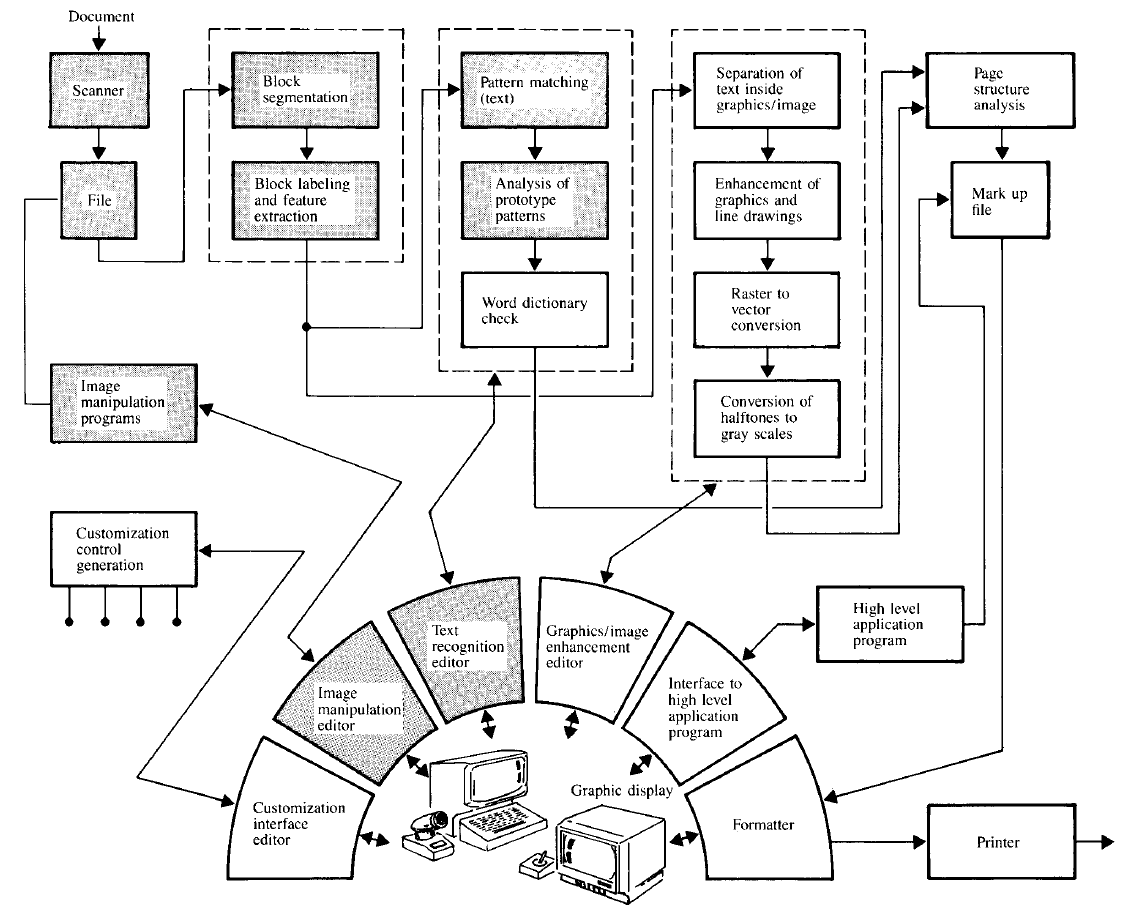
\includegraphics[width=0.9\textwidth]{document_analysis_system.png}
    % \caption[Document analysis system]{Document analysis system~\cite{wong1982document}.}
    % \label{fig:sota:document_analysis_system}
    % \end{figure}
    %%%%%%%%%%%%%%%%%%%%%%%%%%%%%%%%%%%%%%%%%%%%%%%%%%%%%%%%

The content of a document is generally divided into textual and graphical information.
This corresponds to two active research fields, the first one, text recognition aims to convert the text into a character-encoding scheme such as ASCII.
The second one, graphics or symbol recognition, focuses on the recovery of graphical information in documents.
Graphics consist of spatial arrangements of symbols; examples include engineering drawings, maps, architectural drawings, music scores, formulas, tables, charts and some parts of the comic book image content (Figure~\ref{fig:sota:graphics_reco}).

    %%%%%%%%%%%%%%%%%%%%%%%%%%%%%%%%%%%%%%%%%%%%%%%%%%%%%%%%
    \begin{figure}[t]%trim=l b r t  width=0.5\textwidth,  
      \centering
      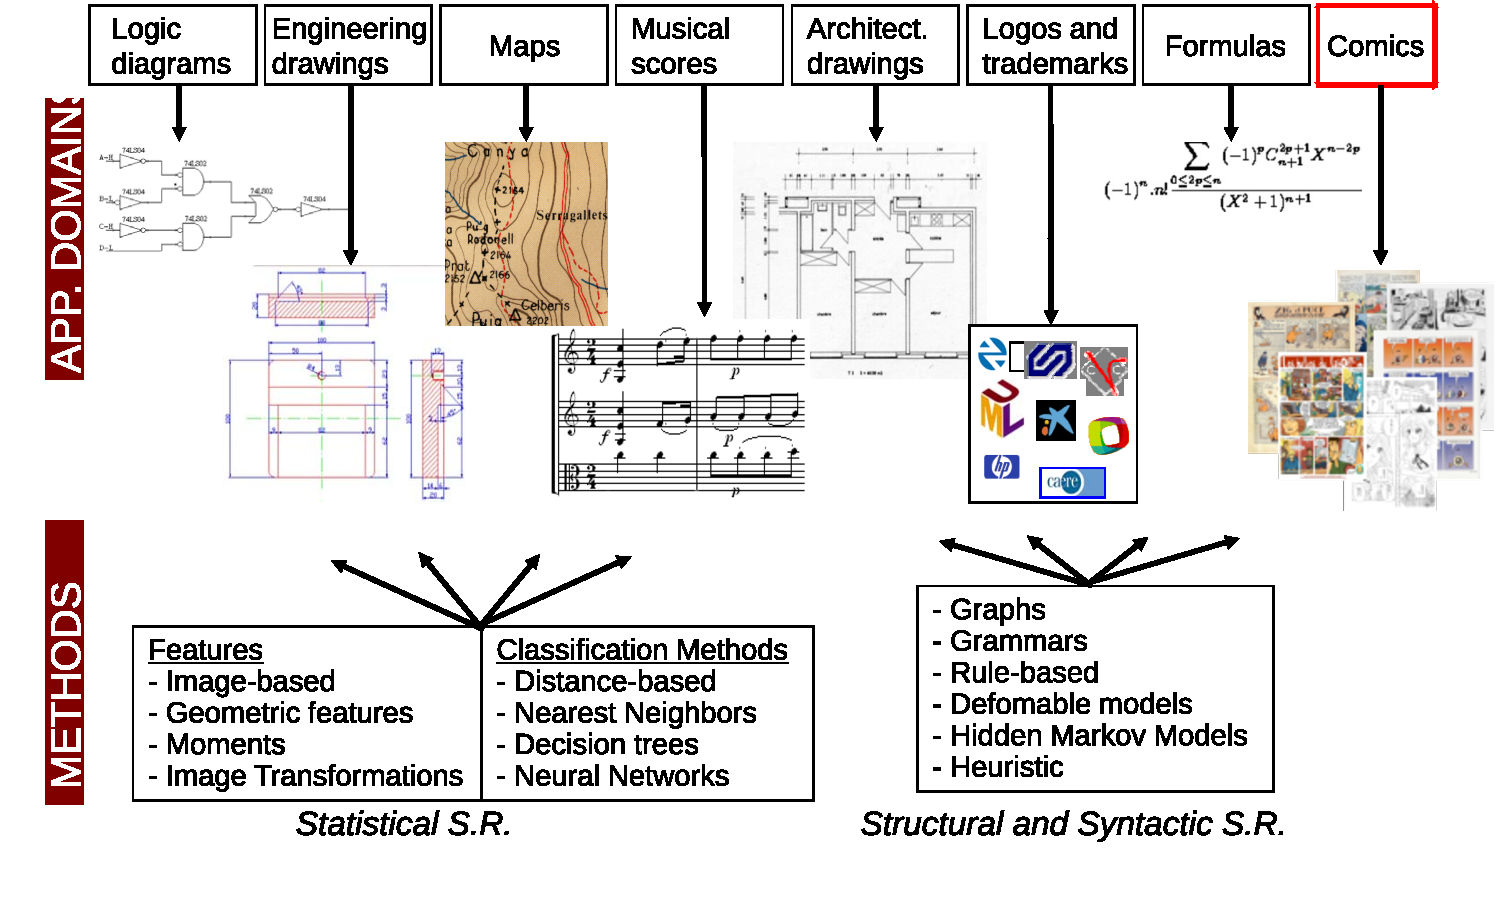
\includegraphics[trim= 15mm 70mm 0mm 0mm, clip, width=0.95\textwidth]{graphics_reco.pdf}
    \caption[Application domains of graphics recognition]{Application domains of graphics recognition.}
    \label{fig:sota:graphics_reco}
    \end{figure}
    %%%%%%%%%%%%%%%%%%%%%%%%%%%%%%%%%%%%%%%%%%%%%%%%%%%%%%%%

Beside its content, a document is usually structured according to its intend of use.
Tang mentioned in 1996 ``A document has two structures: geometric (layout) structure and logical structure.
Extraction of the geometric structure from a document refers to document analysis; mapping the geometric structure into logical structure deals with document understanding''~\cite{tang1996automatic}.
Knowing the structure of the document being processed is always an helpful information that is related to domain knowledge information~\cite{cooperman1998system,breuel2003high}.

Layout analysis consists in segmenting the image into several geometrical blocks that contain the same type of information: text, graphics, table, image, drawing etc.
Then logical information can be retrieved using domain knowledge and the spatial position of the elements (e.g. header and title on the top, page number on the bottom-right corner, reading order).
Layout analysis is not trivial for mixed content documents such as advertisements, posters and comic books.
Those documents use non standard text fonts, size and orientation mixed with graphics, images and logo.% (Figure~\ref{fig:sota:layout_analysis_issues}).

    %%%%%%%%%%%%%%%%%%%%%%%%%%%%%%%%%%%%%%%%%%%%%%%%%%%%%%%%
    % \begin{figure}[t]%trim=l b r t  width=0.5\textwidth,  
    %   \centering
    %   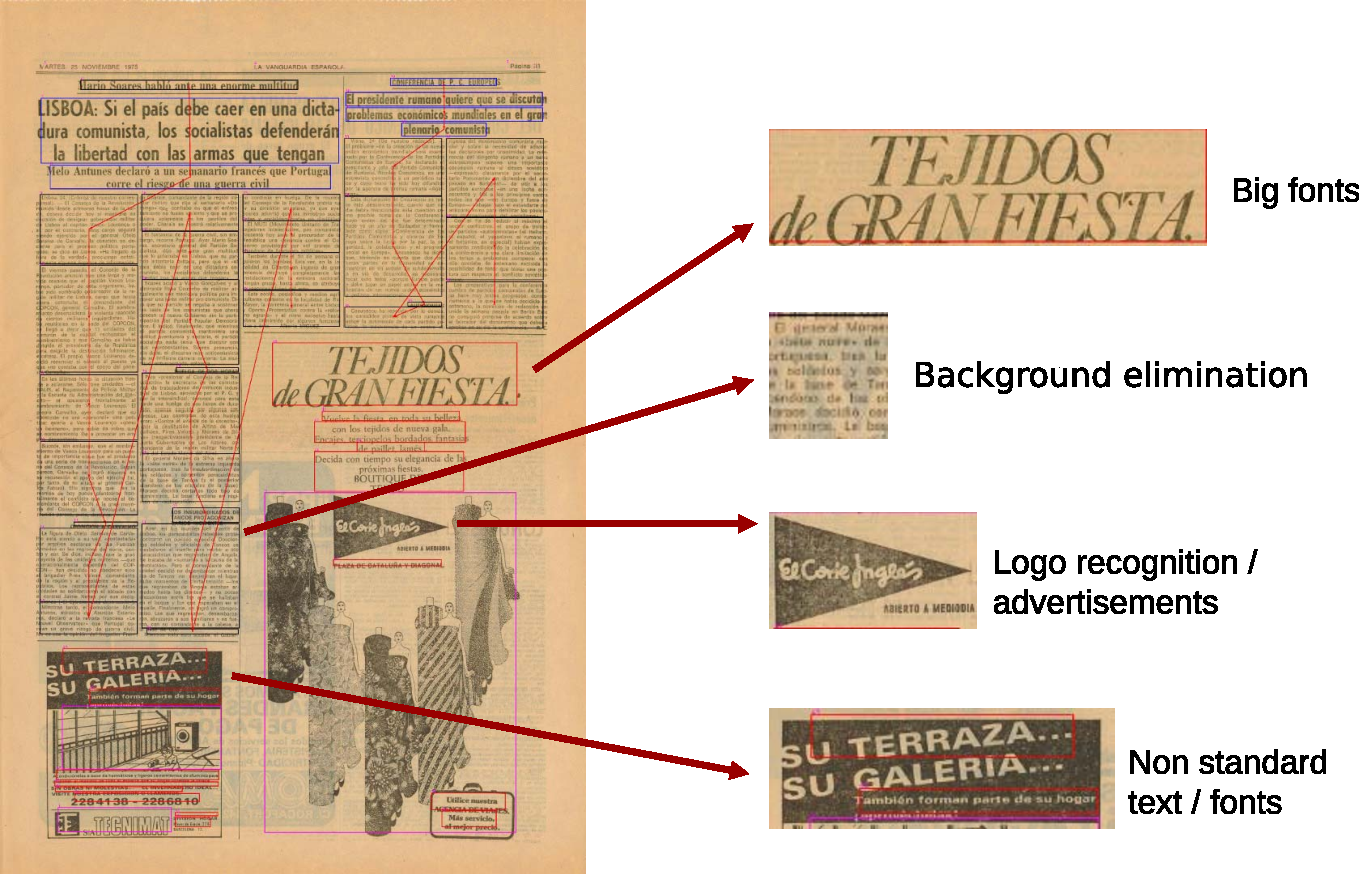
\includegraphics[width=0.8\textwidth]{layout.pdf}
    % \caption[Layout analysis issues]{Layout analysis issues - \emph{Joseph Llados - International Document Image Processing Summer School (IDIPS) 2014}.}
    % \label{fig:sota:layout_analysis_issues}
    % \end{figure}
    %%%%%%%%%%%%%%%%%%%%%%%%%%%%%%%%%%%%%%%%%%%%%%%%%%%%%%%%

Comic book images are composed of text and graphics that can be decomposed as drawings and line drawings.
The diversity of text can be found in comic book images is large.
From speech text which are mostly handwritten to sound effects that are close to drawing sometimes.
Some of the graphics can be assimilated to symbols if we talk about the panels or balloons which have a sort of conventional representation among most of the comic albums.
However, drawings contained in the panel regions do not follow any convention (free art) but contain repeated elements (e.g. comic characters) throughout the album or collection.
This is related to comics art that implies the drawing to be different from others in order to be easily distinguished and recognised by the public.

Comic images are mixed content documents with complex background, especially in the region of panels, that concerns the above mentioned field of research.
Document image analysis being application dependent, we briefly detail the design process of a comic image:

\begin{itemize}
  \item \textbf{Synopsis and scenario} Imagine a story and its decomposition in a sequence of image (storyboard), view angles and format. 
  \item \textbf{Pencil drawing} First rough drawing of the scenario, at this stage, the layout of the page if defined without any details.
  \item \textbf{Inking} The best pencil strokes are inked (permanent) for the final version.
  \item \textbf{Flatting and colouring} Here comes the colours (if any) into all stroke defined regions. Gradient, shadow and other effects are added according to the desired rendering.
  \item \textbf{Lettering and sound effects} Addition of text in reserved areas and sound effects over the graphics at the end.
\end{itemize}

The first challenge of comics book image analysis is to retrieve the layers that corresponds to each step of the comic image design process (e.g. stroke, text, colour).
Processing each layer separately would greatly simplifies layout and content retrieval.
Unfortunately, this decomposition is not obvious because in the final image, the elements are mixed with overlapping and transparency.
Another important issue of document analysis is the noise information added from the creation of the physical document to its digital version.
The main sources of noise are the manual operations variabilities, the degradation over time and the acquisition and storage techniques (Figure~\ref{fig:sota:document_degradation}).


    %%%%%%%%%%%%%%%%%%%%%%%%%%%%%%%%%%%%%%%%%%%%%%%%%%%%%%%%
    \begin{figure}[!ht]%trim=l b r t  width=0.5\textwidth,  
      \centering
      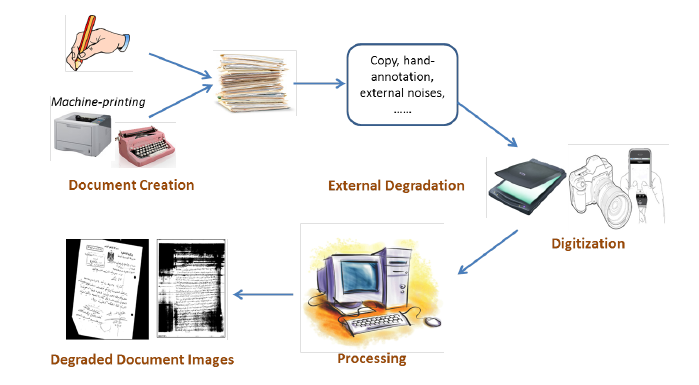
\includegraphics[width=0.85\textwidth]{document_degradation.png}
    \caption[Document degradation sources]{Document degradation sources~\cite{Peng2013Document}.}
    \label{fig:sota:document_degradation}
    \end{figure}
    %%%%%%%%%%%%%%%%%%%%%%%%%%%%%%%%%%%%%%%%%%%%%%%%%%%%%%%%


% Here we briefly detail the most used pre-processing and feature extraction methods related to document image analysis and comics design process.

% \paragraph{Pre-processing} % (fold)
% \label{par:pre_processing}
% Stroke-based images such as comics can be pre-processes is order to extract all the strokes for further analysis.
% Several method from the literature exist, 

% paragraph pre_processing (end)

% \modif{TODO: detail features and classification methods from Figure 2.1?
% Puisque tu en parles par la suite des méthodes de binarisation (globale, locale, binaire), celles sur les composantes connexes, contour actifs, séparation text/graphique ou clustering?



% \begin{itemize}
%   \item Pre-processing methods (\url{http://fr.wikipedia.org/wiki/Segmentation_d'image} FR + EN) -> comic character -> simple PIL with palette + colour L0-smoothing ++
%   \item Feature extraction (textures, outline(), shapes, colour)
%   \begin{itemize}
%     \item Pixel-based (edge, Harris corner, blobs detections)
%     \item Shape-based (thresholding, region growing, connected-component extraction, template matching, Hough transform) 
%     \item Flexible (deformable shapes, active contours)
%   \end{itemize}
%   \item Feature description (to delete?)
%   \begin{itemize}
%     \item Shape-based (compactness, curvature scale space, freeman coding, Fourier transform, invariant moments, texture)
%   \end{itemize}
  
% \end{itemize}
% }



% section document_image_analysis (end)

\section{Comic book image analysis} % (fold)
\label{sec:comic_book_image}

% section comic_book_image (end)

Comics images are mixed content documents combining textual and graphical information to create stories.
Depending on the purpose, the document analysis techniques involved for comics image processing varies a lot between panel, balloon, text and comic character extractions.
The contents of different nature are related to each other to produce a story.
Treating each of the content separately has a limit that can be exceeded in a holistic understanding approach by reaching a higher level of semantic.



\subsection{Panel extraction and layout analysis}
\label{sec:sota:layout_panel}

Panel extraction and ordering have been mainly studied for panel to panel reading.
The need is increasing since the first generation of mobile devices with small screens in colour or B\&W.
In fact, people want to continue reading their favourite comics or manga on the way, without caring kilos of books.
Printed comics require tedious work to be manually scanned and split into screen size parts small enough to avoid zooming and scrolling.

Several techniques have been proposed to automatically extract panels as~\cite{In11}, assuming that panels are small enough elements to be comfortably read on mobile devices.
They are based on white line cutting algorithm~\cite{Duda72,Luyuan2014Automatic,Chan2007Automatic}, recursive X-Y cut~\cite{Han07} or gradient~\cite{Tan07}.
Those methods do not consider empty area~\cite{In11} and border free panels.
These issues have been corrected by connected component approaches~\cite{Arai10} 
%,Rigaud2012LNCS} 
but they are sensible to region that sometimes connect several panels and increase the detection error rate.
Another approach based on growing region and morphological mathematics can remove such connecting elements but also remove information on the panel border~\cite{Ho2012}.
After the region segmentation step, heuristic filtering is often applied to classify panel region according to the size ratio according to the page size, which depends on the page format~\cite{Arai11,Ho2012}.
More recently, new methods have shown interesting results for manga and European comics with different background colours.
They are based on watershed~\cite{ponsard2012ocr}, line segmentation using Canny operator and polygon detection~\cite{Luyuan2014Automatic}, region of interest detection such as corners and line segments~\cite{stommel2012segmentation,Tsai2013Adaptive}.
Panel retargeting have been addressed for manga by Matsui~\cite{Matsui2011}.

Page layout analysis has been studied to calculate the reading order of the panels.
The page layout influences the reader at choosing pathway~\cite{Cohn_2013}, nevertheless few studies~\cite{Guerin2012Ontologies,Ponsard09,Arai2010Automatic} demonstrated the possibility of calculating such Z-path (left-to-right and down) or right-to-left and down (e.g. Arabic, Japanese) according to the arrangement of the panels~\cite{Li2013Comic,Tsai2013Adaptive,Liu2014Automatic}. 

%--------------------------------------------------------------------------------
\subsection{Balloon segmentation and tail detection}
\label{sec:sota:balloon_segmentation}

% Balloons or bubbles are the visual unit that conveys dialogue, either spoken or thought
Balloons are a graphic convention used most commonly in comic books, comic strips and cartoons to allow words (and much less often, pictures) to be understood as representing the speech or thoughts of a given character in the comic\footnote{\url{http://en.wikipedia.org/wiki/Speech_balloon}}.
Balloons are developed into a more-or-less oval shape, with a pointer or tail to indicate to which character they belong~\cite{Goggin2010Rise,Varnum2007Language}.
There are many specialized forms of balloons, either traditional or invented~\cite{Marx2006Writing}.
%Balloons or bubbles are key elements in comics, they link graphical and textual elements and are part of the comics style. 

In comics content understanding, speech balloons present a lot of interest since they offer the links between the textual content and the comic characters providing information about the localization of the characters and the tone of speech.
Apart from being crucial for document understanding, balloon detection is also beneficial in applications such as comic character detection~\cite{Sun2011}, content re-targeting~\cite{Matsui2011}, translation assistance and reading order inference~\cite{Guerin2012Ontologies}.

Few works about balloon extraction have been done until now and mainly closed speech balloon have been studied.
Arai~\cite{Arai11} proposed a blob detection method based on connected component detection with four filtering rules applied to manga analysis.
The rules are based on blob minimum size, white pixel occurrence, inclusion of vertical straight lines and width to length ratio (Figure~\ref{fig:Arai_balloon_extraction_process}).
Another connected component approach proposed by Ho~\cite{Ho2012} uses HSV colour space to make a first selection of bright blobs and then consider as balloons the blobs with a ratio between the text area and the blob bounding box higher than sixty percent.


%%%%%%%%%%%%%%%%%%%%%%%%%%%%%%%%%%%%%%%%%%%%%%%%%%%
 \begin{figure}[!ht]  %trim=l b r t  width=0.5\textwidth,
   \centering
  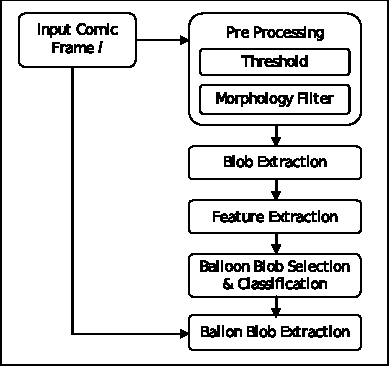
\includegraphics[trim= 0px 0px 0px 0px, clip, width=150px]{Arai_balloon_extraction_process.pdf}
  \caption[Flow diagram of comic balloon detection]{Flow diagram of comic balloon detection using comic blob extraction method proposed by Arai~\cite{Arai11}.}
  \label{fig:Arai_balloon_extraction_process}
 \end{figure}
%%%%%%%%%%%%%%%%%%%%%%%%%%%%%%%%%%%%%%%%%%%%%%%%%%%

The analysis of open balloons with an ``open'' or ``implicit'' contour is quite different than the closed ones which are mainly based on blob analysis and have not been studied before.
In most of the cases, including when contours are implicit, the location of text is generally a good clue to guess where the balloon is.
The problem of speech balloon outline detection can therefore be posed as the fitting of a closed contour around text areas.
The active contour~\cite{Kass1988} model is a deformable model, also known as snake, which tries to minimize an energy associated to the current contour as a sum of an internal and external energy.
Kass~\cite{Kass1988} proposed the original energy functions able to shrink around an object contour, Xu~\cite{Xu1998} proposed the Gradient Vector Flow external force to attract snake from further and handle broken object edges and subjective contours.
% GVF is adapted to our application of non-closed (broken object).
Another extension was proposed by Cohen~\cite{Cohen1991} to make the curve behave like a balloon which is inflated by an additional force.
 %The initial curve needs no longer to be close to the solution to converge''. %We use this last method extension for speech balloon segmentation and customize it in order to detect open balloons.
%Dimos_v1: I don't understand this sentence. multi-resolution contours have been studied to speekd up the multi-resolution model???
Finally, active contour in a multi-resolution context have been studied to speed up the process on multi-resolution image and the multi-resolution model itself~\cite{Leroy1996}.
% We adapt the active contour framework to the domain of comics in~\ch{chap:be}.

% , we propose first approaches in~\ch{chap:be}.
% , balloon contour and tails have not been studied before, we propose first approaches in~\ch{chap:be}.

Balloons provide also an extra information about speech tone according to the different patterns which are along the contour of the balloon.
The shape of the balloon does not provide a lot of information about how the text is spoken, it is more related to the style of the comics and the structure of the panel.
Therefore, we focus on contour classification methods.
In the literature, contour classification is strongly related to shape classification purposes~\cite{sun2005classification,liu1990partial}.
It has been applied for video~\cite{kuhne2001motion,richter2001contour,bader2009}, trademark retrieval~\cite{leung2002trademark}, speech recognition~\cite{grigoriu1994automatic}.
Also, wavelet decomposition~\cite{tieng1997recognition} and invariant moment~\cite{mukundan1998moment}. 
% We propose a first approach in~\ch{chap:be}.

From our knowledge, tail detection have not been studied before, we propose to analyse the contour patterns in order to locate the tail and then perform a local analysis to find its direction (Section~\ref{sec:se:from_balloon_to_tail}).

Balloon classification and tail detection are also important in a context of dialogues and emotions understanding~\cite{millidge2009comic}.



% chapter chap_be (end) ~\ref{sub:be:segmentation}.

%We proposed a first method to extract non closed balloons based on active contours initialized around text areas~\cite{rigaud2013active}, see section~\ref{sub:be:segmentation}.
% This method is able to approximate the contour region, even when it is not printed, based on a domain knowledge which is the mean distance between the balloon contour and the text it contains. 

% A balloon is a spatial container of information that is related to a protagonist using a specific element: the tail.
% The tail is often represented by a discontinuity on contour of the balloon towards the concerned protagonist.
% From our knowledge, there is no work about tail extraction and description in the literature.




\subsection{Text extraction and recognition}
\label{sec:sota:text}

% \begin{itemize}
% 	\item \url{/Text_graphic_separation/2002_Bernhaupt_Using ArtificialNeuralNetwork as image segmentation : application on comics} 
% \end{itemize}

Text localization in real scenes and video frames is an active research topic~\cite{Jung04,ShahabICDAR2011Robust,KaratzasICDAR2013Robust}.
However, applying existing real scene text detection methods to comics would not be optimal to cope with all the different types of text that are combined in comic book documents (e.g. typewritten, handwritten, graphic sound).
If we consider typewritten text, the most similar application to comics is car plate recognition because the text is in a salient and contrasted area with a complex background around the plate such as speech balloon for comics~\cite{anagnostopoulos2008license}.
The documents that have attracted of lot a attention are newspaper, administrative documents, cheques, maps, floor plans and engineering drawings.
Nevertheless, text localization in comic images opens up several interesting applications such as image compression~\cite{Su11}, OCR training and also translation, speech synthesis and re-targeting to different mobile reading devices~\cite{Matsui2011}.

Comics differ from classical documents in that they comprise complex backgrounds of a graphical nature. Furthermore, they belong to the class of non-structured documents meaning there is no regular structure present for the prediction of text locations and no layout method applicable.
Comics being unstructured graphical documents, combine the difficulties of both domains, making the task of text localization especially challenging.

Text localization in complex images has been previously studied in scene images~\cite{Weinman09,Epshtein10,Neumann12} and~\cite{Wang10,Meng12}, video sequences~\cite{Wonjun09,Shivakumara09} and digital-born images (Web and email)~\cite{Karatzas07}. 
Text localization in unstructured documents has been studied for teaching boards and slide show presentation~\cite{Oliveira10,Vajda2012Method,Nguyen2013BagOfSubjects}.
However, text localization in documents which are both unstructured and have complex background has received relatively little attention~\cite{Clavelli09}.

% Nevertheless, plates are typewritten with a fixed length.
%From our knowledge, only text localization has been studied, no text segmentation or text recognition yet. This is probably due to the lack of dataset and ground truth to evaluate the algorithms.
Few works concern text extraction in comics, they all rely on speech balloon regions.
Bottom-up approaches use connected component which often relies on the segmentation step~\cite{ponsard2012ocr}.
Su~\cite{Su11} uses Sliding Concentric Windows as text/graphic separation and then apply mathematical morphology and a Support Vector Machine (SVM) classifier to classify text from non-text components. 
%Morphological operations are performed with a fixed mask size, the method is orientation and resolution dependent.
% In~\cite{Rigaud2013VISAPP}, we proposed a adaptive binarisation process based on the Minimum Connected Component Thresholding followed by a text/graphic separation based on contrast ratio and text line grouping, see~\ch{chap:te}.
% Previously, we proposed a k-mean classification of the 
Li~\cite{Li2013Unsupervised} proposed unsupervised speech text localization for comics that trains a Bayesian classifier on aligned connected component and then detect the rest of the text using the classifier for text/non text separation.
 
% Rigaud~\cite{Rigaud12} %~\cite{Rigaud12}
% make use of ``the median value of the border page pixels'' to binarize the image, extract CC and then classify them into ``noise'', ``text'' or ``frame'' (based on CC heights). This method assumes that the page always contains text and that the text background colour is similar to the paper background. 

Top-down approaches starting from balloons (white blobs) detection followed by mathematical morphology operations have been proposed by Arai~\cite{Arai11}, Yamada~\cite{Yam04} and Sundaresan~\cite{Sundaresan2012Text}.
From our knowledge, there are no published work concerning graphic sounds (onomatopoeia) and illustrative text extraction.

Text recognition applied to comics is really challenging because it includes most of the difficulties from text recognition in document analysis domain if we consider all the type of text that composed the comics.
From typewritten to handwritten and free-form text in uniform to complex background including image noise, text deformation and overlapping.
Nevertheless, Ponsard~\cite{ponsard2012ocr} solved a sub part of the problem by focusing on speech text of a single typewritten font and language for which an OCR system is trained for.


\subsection{Comic character detection}
\label{sec:sota:comic_character}

% \begin{itemize}
	% \item Garfield character detector based on colour histogram \url{/PhD/Biblio_LINK/Object_detection2013_Landry_colour Based Comic Strip Character Recognition.pdf}
	% \item \url{2011_Matsui_Interactive manga retargeting - siggraph11.pdf}
	% \item \url{object/2012_Takayama_FACE DETECTION AND FACE RECOGNITION OF CARTOON CHARACTERS USING FEATURE EXTRACTION}
	% \item \url{object/2007_MASTER_Cheung_Face detection and face recognition of human-like characters in comics}
	% \item Stoke images \url{Object_detection/2010_THESIS_Ta_phuong_inexact_graph_matching_application_to_stroke_images_comics.pdf}
% \end{itemize}


Human detection in computer vision field has been largely studied during the past decades, mainly based on greyscale image and gradients. colour information is rarely relevant for human detection because of clothing and skin colour difference. In videos, moving regions are often used as region of interest.

Although, comics are often a reproduction of human life situations, it is a domain where we can not directly apply human detection based methods.
The main difference is that comic characters (e.g. protagonist, hero) are hand drawn and therefore more variant in terms of deformation, shape and appearance than real life humans (Figure~\ref{fig:sota:tarzan}).
% Comics are composed by a sequence of static snapshots telling a story like a video at a very low frame rate, where we want to detect similar objects. 
In coloured comics, the colour information gives the identity of characters and plays a main role for character spotting with speech balloon positions. 
The simplistic character design allows for easy identification and representation and goes along with how human process visual information~\cite{ahmadimpactsOfManga,medley2010discerningPictures,cohn2010limits}.
%Comics characters are often described using colours while human are described using head feature (e.g. brown hair, blue eyes) because it is the only part that does not change in every day life. 
This is a big difference compared to natural images and human detection, since comics are designed in a way that the information (e.g where are the comic characters, who is talking, where is it going) can be quickly found.% Famous people also use this technique to be easily recognize in video show for example (professional identity).

%%%%%%%%%%%%%%%%%%%%%%%%%%%%%%%%%%%%%%%%%%%%%%%%%%%
 \begin{figure}[!ht]	%trim=l b r t  width=0.5\textwidth,
 	 \centering
 	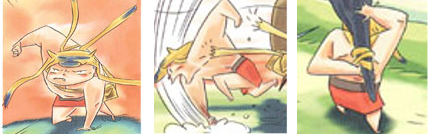
\includegraphics[width=220px]{figs/prunelle.png}
 	\caption[Illustration of the diversity of comics character postures]{Examples of comics character postures. This example shows deformation, pose, rotation, translation and occlusion variations. Image credits: Prunelle, la fille du cyclope, Vicky Portail-Kernel and C\'{e}dric Kernel, Ankama, 2010.
}
 	\label{fig:sota:tarzan}
 \end{figure}
%%%%%%%%%%%%%%%%%%%%%%%%%%%%%%%%%%%%%%%%%%%%%%%%%%%

Recent studies have been published for partial manga copy detection~\cite{Sun2010}, mainly based on shape information because of the absence of colour information.
This work has been extended to Manga copyright infringement protection~\cite{Sun2009Detecting,Sun2013IJDAR} using Maximally Stable Extremal Regions (MSER)~\cite{matas2004robust} or faces~\cite{Viola2004robust} for region detection and Histogram of Oriented Gradients (HOG)~\cite{Dalal05} as region descriptor.
A recent study discuss the local feature extraction and the approximate nearest neighbour (ANN) search~\cite{Iwata2014StudyManga} .
This work shows good results for manga part retrieval which is a subset of the whole comics world.
% In our work we focus on a complementary subset, corresponding to coloured comics analysis.

Coloured comics may be compared to cartoon images sequence, for which a first work based on HOG, SVM and colour attributes has been published in 2012~\cite{Khan12}.
Preliminary work about cartoon and comics faces recognition have been carried out by Kohei~\cite{Kohei2012} and Cheung~\cite{cheung2008face}.
More recently, graph theory has been used to find redundant colour structure in order to automatically localize the most frequent colour group apparition and label them as main characters~\cite{HoGREC2013}.
The thesis of Ta~\cite{TAPhD2010} (section 1.1 and 1.2) gives a good overview about stroke-based image analysis similar to comics, it defines the issues of poor information, occlusion, deformation, inter-class and intra-class variations, scale, spatial and/or temporal relations and structured data.
Ta~\cite{TAPhD2010} also mentions that ``story board scene understanding still remains an open problem, few results are available in the literature about stroke images''.

Another work uses HOG descriptor with redundant information classification to also find the most frequent elements~\cite{SunICDAR2013}.
% It has been improved  
Both graph and descriptor based methods need an image preprocessing step to remove irrelevant redundant elements such as text and speech balloons.

Other interesting approaches try to automatize comic generation~\cite{Tobita2010Comic,WangHYYC12} using image cartoonification and script analysis.

%%%%%%%%%%%%%%%%%%%%%%%%%%%%%%%%%%%%%%%%%%%%%%%%%%%%%%%ù

% Human body and face extractions in real scene image have progressed a lot during the last decades. 
% Nevertheless, the few studies that are related to comics shown that human detection techniques are not appropriate for comics character or need to be trained for specific comic types.
% Those studies concerns the fraud detection in mangas~\cite{Sun2013IJDAR}, cartoon classification~\cite{Khan12} and the detection of the main characters using redundancy information~\cite{SunICDAR2013,HoGREC2013}.
% Preliminary work about cartoon and comics faces recognition have been carried out by Kohei~\cite{Kohei2012} and Cheung~\cite{cheung2008face}.

%We recently proposed~\cite{RigaudDAS2014} a query by example approach that ask the user to select a part of the object he is looking for in one comics image and the system retrieves it automatically everywhere in all the pages of the comics album, assuming that they have been digitized under the same conditions.


\section{Holistic understanding} % (fold)
\label{sec:sota:holistic_understanding}

One of the original goals of image or graphical document analysis was to fully understand the content of any image~\cite{Lamiroy2014Handbook}.
This requires solving several sub-tasks simultaneously, for instance region detection, labelling of meaningful regions and semantic understanding using layout analysis.
In the past, researchers have developed classifiers for tackling each of these sub-tasks independently~\cite{Mao2003Document}.
However, these sub-tasks can help each other.
For instance, in a comics page, if we know the panel positions, then we can make a better guess at the location of the comics characters (they are usually inside the panels).
However, it is not easy to combine different related sub-tasks together.
Previous works concern real scene image analysis~\cite{Blaschke2014Geographic}, retrieval~\cite{Sciascio2011Structured} and understanding~\cite{Li2012Toward,Fidler2012Describing}, medical image annotation using description logic and inference engine~\cite{Hu2003Ontology}, object-based image retrieval~\cite{Mezaris03anontology,Sarwar2013Ontology} (between keyword-based and query-by-example) and image interpretation~\cite{Hudelot2008Fuzzy,Ogier2000Semantic} that mentions the importance of using topological information, distances, directional relative position and much complex relations such as ``between'' and ``surround'' and ``among''.
Also, Geographic Object-Based Image Analysis (GEOBIA)~\cite{Blaschke2014Geographic} makes extensive use of ontologies to interpret maps.

%{\bf ADD} background about document understanding and drawing retrieval (OK: cadastral map).

Recently, comics book images have been also considered.
An ontology of comics has been proposed from a philosophical approach~\cite{Aaron2011}, a semantic annotation tool~\cite{Hermann2012Guided} makes use of previous knowledge and consistency information to suggest new knowledge to the user in a interactive way.
Spatial inferences have been used to infer the comic books reading order, for panel in the page and balloon in the panel~\cite{Guerin2012Ontologies}. 
In~\cite{Sciascio2011Structured}, they highlight the benefit of using contextual information of simple object to build more complex ones.
% From our knowledge, there is no framework for document understanding in the literature that infers new knowledge iteratively and without user interaction (unsupervised).

% section holistic_understanding (end)

\section{Existing applications}
\label{sec:sota:applications}

% \begin{itemize}
	% \item Voice + comic: people tell the comic story and sell them \url{http://vomic.shueisha.co.jp/}
	% \item Comic Chat is a working program, allowing groups of people to communicate over the Internet see \url{2006_Kurlander_Comic_Chat.pdf}
	% \item \url{2010_Tobita_Comic Engine: Interactive System for Creating and Browsing Comic books with Attention Cuing.pdf}
	% \item Comic life: turning your photos into a comic \url{http://plasq.com/}
	% \item Online interactive creation of comics \url{2009_Lopes_Calligraphic Shortcuts for Comics Creation.pdf}

	% \item Software for scripting comics, to define the interactions, time, zoom and region for a kind of video export \url{2012_Raulet_A Sketch-based Interface to Script Comics Reading.pdf}

	% \item Movie to comics: ... the first three factors determine balloon size, and the last factor determines balloon shape ... Emotion can be further exhibited by shape of balloon [1] \url{/PhD/Biblio_LINK/Speech_balloon_analysis/2013_Chu_Optimized Speech Balloon Placement for Automatic_comics_generation.pdf}
% 	\item OCR Manga Reader \url{https://play.google.com/store/apps/details?id=com.cb4960.ocrmr&hl=en}
% 	\item Capture2Text \url{http://capture2text.sourceforge.net/}
% \end{itemize}


Comic books are a graphic art form combining text and images to tell a story.
Comics are now used in a wide variety of styles, not only on paper (e.g., magazines, newspapers, TV show) but also as electronic content (smartphone apps, e-books, websites).
Comics are one of the most popular and familiar forms of graphic content.
People read comics easily and learn many things, so even children can learn about cultures and trends, among other things, through comics even unconsciously.

From this background, we can divide comic-based computer systems into two categories.
One type would be using comics to represent complex information such as online communication in a form of comics~\cite{Kurlander1996} and generating video or story log summaries~\cite{Uchihashi1999Video,Alves2008So,Shamir2006Generating} (computer graphics domain).
Also, it is possible to listen to manga~\cite{Vomic} which have been recorded by people reading the story or to use mobile app for automatic translation~\cite{OCRMangaReader,Capture2Text} (requires user text selection).
These systems are useful to add value to the content while making it more funny and interesting.
The other category concerns the comic design by enabling novices to create comics  interactively using a computer for augmenting an individual user's memory~\cite{SumiSNM2002Comic}, turning photo albums into a comic~\cite{ComicLife3,Chu2013Optimized}, making comic-like video~\cite{Raulet2011Sketch}, making collaborative comics~\cite{Ricardo2009Calligraphic} and exchanging rich message~\cite{Salovaara2007Appropriation}.




\section{Conclusion}
\label{sec:sota:conclusion}


% \begin{itemize}
	% \item Copy/paste from previous publications
	% \item Demonstrate that I understand the topic
	% \item Conclusion and critics

	% \item Navigating comics: an empirical and theoretical approach to strategies of reading comic page layouts \url{2013_Cohn_navigating_comics.pdf}
	% \item 2013 SIGRAPP poster \url{2013_Tsai_Adaptive Manga Re-Layout On Mobile Device.pdf}
% \end{itemize}

Some of the challenges of comics image analysis can be highlighted from the above state-of-the-art reviews.
First, comics image suffer from noise as any other document image processing.
It comes from hardware processes (e.g. drawing techniques, printing and digitization) and software (e.g. image compression).
So efficiently handling noise is crucial for image analysis and understanding.
Knowing the design process of the comics creation helps for image denoising.
Second, according to the results of the reviewed methods, we can order them by level of difficulty, from the simplest to the hardest: panel, balloon, text, comic character and holistic understanding of an image or album.
% \modif{add comparison table about genericity, processing time, complexity???}.
Third, most of the works in the literature use different copyrighted images which can not be shared publicly.
Moreover, the authors usually do not share their code.
This is a key issue for researchers which can not share, reproduce and compare results on identical data in a collaborative way.
This is one of the reasons that retains comics analysis to progress as fast as other field of research of document analysis.


In the next chapter, we are going to present a sequential content extraction approach that profits from the relations between elements to guide the retrieval process.
We first process panel and text region extraction followed by speech balloon and tail segmentation.
Then, speech balloon tail indications are used to compute a comic character region of interest according to the spatial organisation of previously extracted elements in each panel.



%the first comics image dataset and ground truth publicly available for researchers. It is a selection of hundred pages from more than twenty different albums from America, Japan and Europe.
% The construction of the dataset and ground truth and a quality assessment test are detailed.
% The hash based technique helps to reduce search space considerably and perform the subgraph matching (symbol spotting) faster.

% The first approach profits from the relations
% between elements to guide the retrieval process. For instance, the panels are first extracted then balloons containing text that are inside panels and finally comic character regions of interest are defined from the speech balloon tail indications.

\chapter{Sequential information extraction}%Panel extraction}
\chaptermark{Sequential information extraction}
\label{chap:sequential}
\graphicspath{{./chapters/3-sequential/figs/}}

% Abstract -------------------------------------------------------------------------------------------------------------------------------------------
This chapter presents a sequential information extraction approach for comic book content retrieval.
The sequence of extraction starts from elementary elements such as panel and text that initiate further processing.
Once the text regions are discovered, we use them as seeds to search for balloon and then analysis the balloon contour to detection the tail.
From the tail, comic character regions are computed according to previously extracted element positions.

% -------------------------------------------------------------

\section{Introduction} % (fold)
\label{sec:introduction}

In comics art, the page structure depends on the author style which is why so many different structures and drawing types exist.
It is unavoidable because it gives an unique graphical identity to the comics and contributes to attract the curiosity of the readers.
Despite the differences of style, the comics drawings follow ``general use'' characteristic intrinsically to the design process (see section~\ref{??}).
% Relations between elements and inking process are particularities that we we rely on when processing such images. surrounded by a black stroke.
For instance, the inking process requires to magnify the main strokes and then colourize.
We propose to rely on this main strokes to automatically extract non coloured image content (e.g. panel boundary, text, speech balloon background) using a connected-component labelling~\cite{Szeliski2010Computer} approach.
Then, the analysis of speech balloon contour allow to detect the tail precisely and its direction is used to compute the of region of interest of comic characters.
In this section, all the processes here are related to each other, for instance, the text extraction output is the input of the balloon extraction process.


% section introduction (end)

\section{Panel and text} % (fold)
\label{sec:se:panel_and_text}


This section proposes a method to automatically extract the panels and text regions contained in comics pages.
This method is not limited to text which is included into speech balloon such as most of the work in the literature.
Here we consider all the text regions of the image using connected-component labelling approach and k-means clustering.

% \p{Methodology} % (fold)
% \label{sec:se:methodology}

To be clustered, the connected components have to be extracted from the image first.
A commonly used method is to segment the original image pixels into two categories called foreground and background (binary segmentation).
The foreground category corresponds to the set of pixels of interest, here the pixels of the panel border strokes.
This is usually performed using binary segmentation techniques which assign each pixel to one of the two categories.
From the foreground pixels, a structural analysis (connected-component labelling) allows us to group ``connected'' pixels into components according to their connectivity.
 % that are connected (black pixels over white background).
% Then, the ROI are defined as the set of the connected-component bounding boxes (rectangles).

% Connected components labelling scans an image and groups its pixels into components based on pixel connectivity.
% All pixels in a connected component share similar pixel intensity values and are in some way connected with each other.
Connected component approaches are commonly used for stroke-based document analysis, there are also simple and computationally efficient.
Once extracted, their can be clustered according to different features (e.g. size, shape ,colour, location).
We use this approach to extract panels and text which can be easily differentiated using size and topological information.
% with meaningful names ``noise'', ``text'' and ``panel'' using a classifier with three cluster using discriminant features for instance.
% The originalities of this paper are frame segmentation, with or without box, and out-of-balloon text segmentation that can be extracted by CC algorithm.
% The aim of the pre-processing step is to separate background and content of the page in order to focus on the content later. Several processing are implemented in order to apply CC algorithm, and then, to extract the bounding boxes. It can be resumed as follows:
The process can be summarize as bellow:
  \begin{enumerate}
	\item Image segmentation
	\item Connected-component extraction
	\item Connected-component clustering
	\item Candidate regions pruning
  \end{enumerate}
% paragraph principle (end)


\paragraph{Image segmentation} % (fold)
\label{par:se:image_segmentation}

The first step consists in a colour to grey level (3 to 1 channel) conversion.
Several methods exits for such conversion, combining the three channels of the red, green, blue (RGB) colour space with different preponderation as given in~\cite{Pratt91} or using one channel from the Hue Saturation Lightness (HSL) or Value (HSL) representation of the RGB colour space.
Here we use the lightness channel because the panel border strokes and text are usually darker than other element in the image, including the background. 
Then, a global binary segmentation (figure~\ref{fig:se:binary_img}) is applied with a threshold computed from the median value of the border page pixels where pixels with a value lower than the median value are considered as part of the foreground (we are interested in black strokes).
We assume that the border pixels of the page are representative of the page background (depending on the digitization process).
If the median value is closer to ``black'' than ``white'' grey level, then, image inversion is applied and we redo the complete process in order to always get a white background at the end of this step.
% This pre-processing is more robust than~\cite{Arai11} who assumes that the page is always white and uses a constant threshold.
The binary conversion step is very important for the rest of the method because the background part will not be considered for further processing. %Sometimes, parts of text can be merged with background if their background intensity level is higher than the binarisation threshold.


\paragraph{Connected-component extraction} % (fold)
 \label{par:connected_component_extraction}
 
The connected-component algorithm is applied on the binary image and the bounding box of each of the black component is computed to facilitate subsequent processing (Figure \ref{fig:se:cc_bounding_box}).
We do not consider white connected-component here because we expected panel border and text elements to be darker than other elements in the page (segmented as black region).

	%%%%%%%%%%%%%%%%%%%%%%%%%%%%%%%%%%%%%%%%%%%%%%%%%%%
	\begin{figure}	%trim=l b r t  width=0.5\textwidth, 
	  \centering
		%\includegraphics[height=60mm]{figure/BUBBLEGOM_T01_P007_crop.jpg}
		%\includegraphics[trim= 0mm 0mm 0mm 0mm]{figure/BUBBLEGOM_T01_P007.jpg}
		\subfloat[Binary segmented image]{\label{fig:se:binary_img}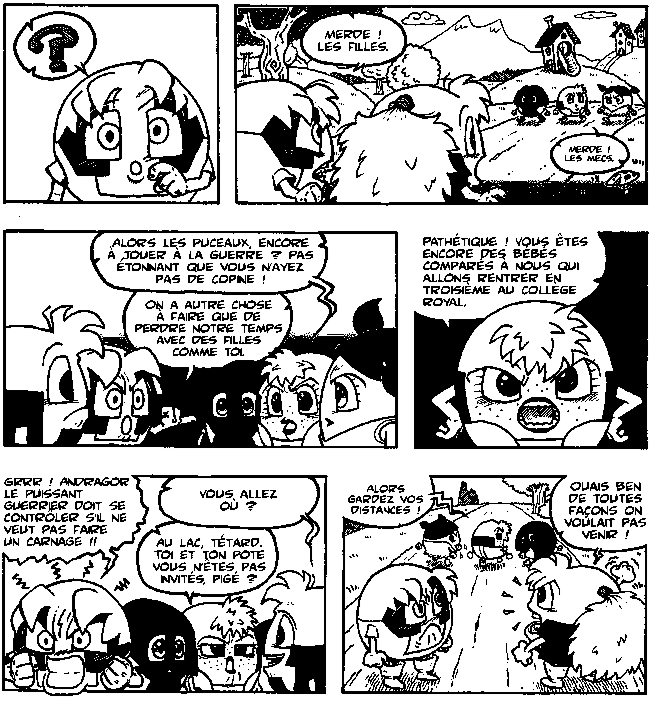
\includegraphics[trim= 0mm 0mm 0mm 0mm, clip, width=0.4\textwidth]{binary.png}}	\hspace{2em}
		\subfloat[Connected-component bounding boxes]{\label{fig:se:cc_bounding_box}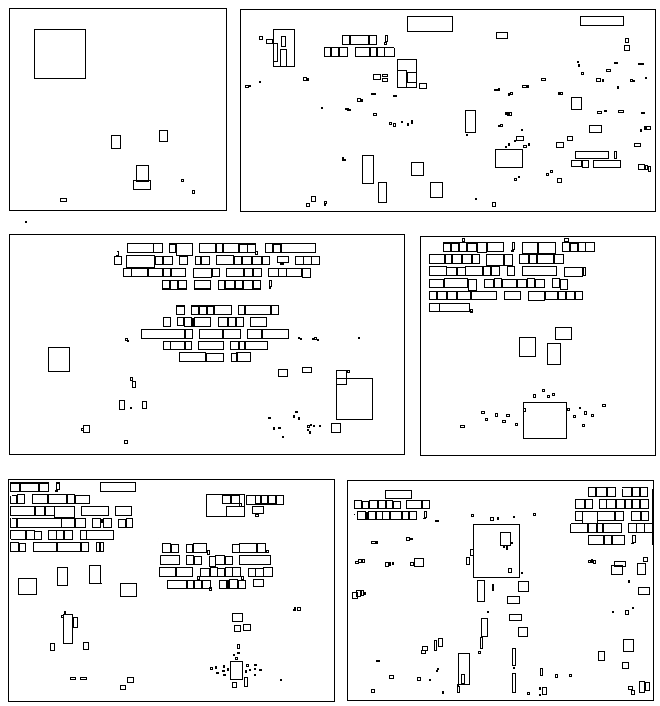
\includegraphics[trim= 0mm 0mm 0mm 0mm, clip, width=0.4\textwidth]{roi.png}}
		\\
		\subfloat[Panel cluster]{\label{fig:se:frame_unrecognized}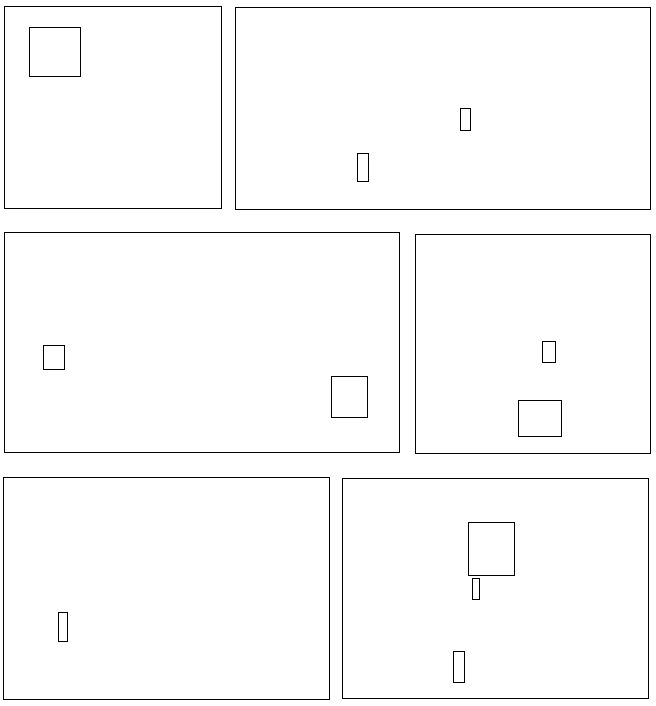
\includegraphics[trim= 1mm 0mm 0mm 0mm, clip, width=0.4\textwidth]{frame_unrecognized.png}}	\hspace{2em}
		\subfloat[Text cluster]{\label{fig:se:frame_cleaned}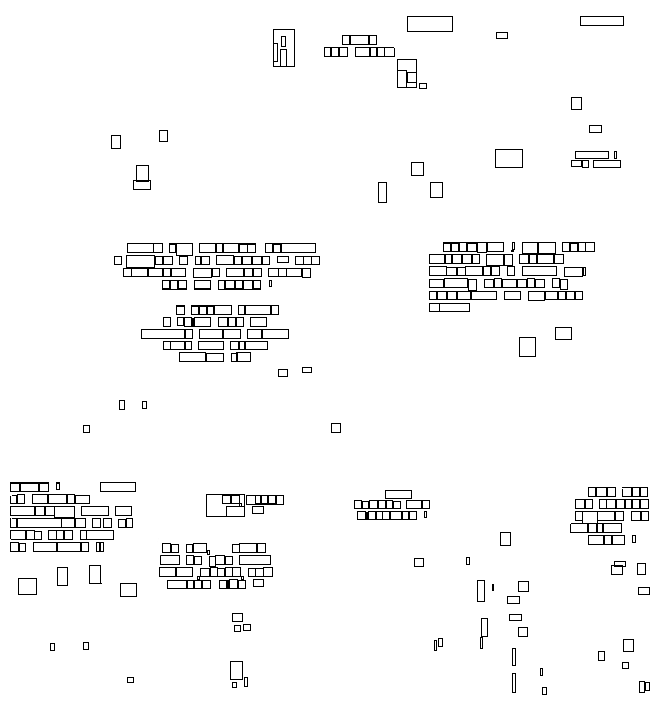
\includegraphics[trim= 1mm 0mm 0mm 0mm, clip, width=0.4\textwidth]{text.png}}
		  \caption[Panel extraction process]{Panel extraction process. Image credits:~\cite{Bubble09}.}
		  % \label{fig:se:binary_to_bounding_box}
	\end{figure}
	%%%%%%%%%%%%%%%%%%%%%%%%%%%%%%%%%%%%%%%%%%%%%%%%%%%

% paragraph process (end)

 % paragraph connected_component_extraction (end) 


\paragraph{Clustering} % (fold)
\label{par:clustering}
By looking at the figure~\ref{fig:se:cc_bounding_box}, we can clearly see that the bounding boxes of the panel are bigger than the others.
Also, they include more regions than others.
Classifying those regions according to their size allows us to classify panel and text region at the same time while ignoring noise information.
Knowing the number of cluster facilitate the clustering, here 
% The classification of connected-component heights using k-means algorithm. 
%We define the set of component bounding boxes $R = \{R_1, R_2, ... , R_n\}$.
we set the number of clusters $k=3$ according to the domain knowledge of comics.
They aim to reflect the ``panel'' (the highest), the ``text'' (medium height) and the ``noise'' (few pixels height) as shown on figure~\ref{fig:se:histo_roi}.
One of the most popular clustering algorithm is k-means clustering method.
It aims to partition $(x_1, x_2, ...,x_n)$ observations into $k$ clusters ($k <= n$) $S=\{S_1, S_2, ..., S_k\}$ in which each observation belongs to the cluster with the nearest mean.
This optimisation problem is formulated as formula~\ref{eq:se:k-means}.

\begin{equation}
	arg min \sum\limits_{i=1}^k \sum\limits_{n_j \in S_i} ||x_j - \mu_i||^2
	\label{eq:se:k-means}
\end{equation}
where $\mu_i$ is the mean of points in the cluster $S_i$.

This clustering is performed dynamically on each image which makes this method parameter-free (given a number of cluster) and invariant to page format and resolution.
% Indeed, the height-based classification is not page size dependent unlike~\cite{Khoi11,Arai11}, and the number of pixels for each ROI is proportional to the page resolution (do not bias the classification).

	%%%%%%%%%%%%%%%%%%%%%%%%%%%%%%%%%%%%%%%%%%%%%%%%%%%
	\begin{figure}[!ht]	%trim=l b r t  width=0.5\textwidth, 
	  \centering
		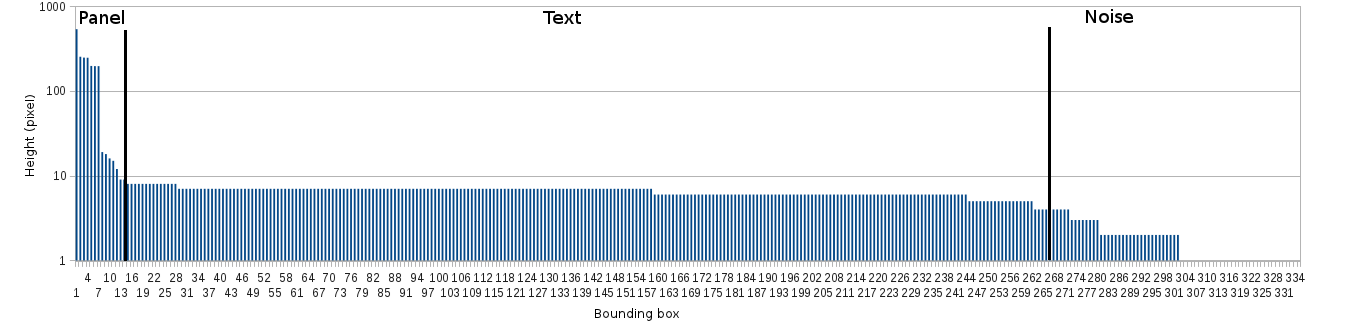
\includegraphics[trim= 5mm 0mm 10mm 0mm, clip,width=1.0\textwidth]{Histogram_en.png}
		\caption[Descendant histogram of the connected component bounding box heights]{Descendent histogram of the bounding boxes in figure~\ref{fig:se:cc_bounding_box}. Vertical black lines represent an example of three cluster limits labelled as ``panel'', ``text'' ``noise'' .}
		\label{fig:se:histo_roi}
	\end{figure}
	%%%%%%%%%%%%%%%%%%%%%%%%%%%%%%%%%%%%%%%%%%%%%%%%%%%

This method assumes that the image is highly contrasted and contains a high disparity between stroke sizes otherwise the binary segmentation or the clustering process may fail.

\paragraph{Pruning} % (fold)
\label{par:se:pruning}
The results from the clustering operation can be pruned using domain knowledge.
First, a panel is rarely included in another so 
% Components clustered as panel sometimes include other panel which is really rare in comics.
we take out components which are included in other regions of the panel cluster.  
% After the classification step, the second characteristic of panel is used in order to keep only the components that are not overlapped by others.
Given the set of component bounding boxes from the panel cluster $R = \{R_1, R_2, ... , R_n\}$, we filter out panel candidates that do not verify this relation $R_i\notin{R_j} \forall j, i \neq j$ (Figure \ref{fig:se:frame_candidates} and~\ref{fig:se:frame_cleaned}).

	%%%%%%%%%%%%%%%%%%%%%%%%%%%%%%%%%%%%%%%%%%%%%%%%%%%
	\begin{figure}	%trim=l b r t  width=0.5\textwidth, 
	  \centering
		\subfloat[Candidate panels]{\label{fig:se:frame_candidates}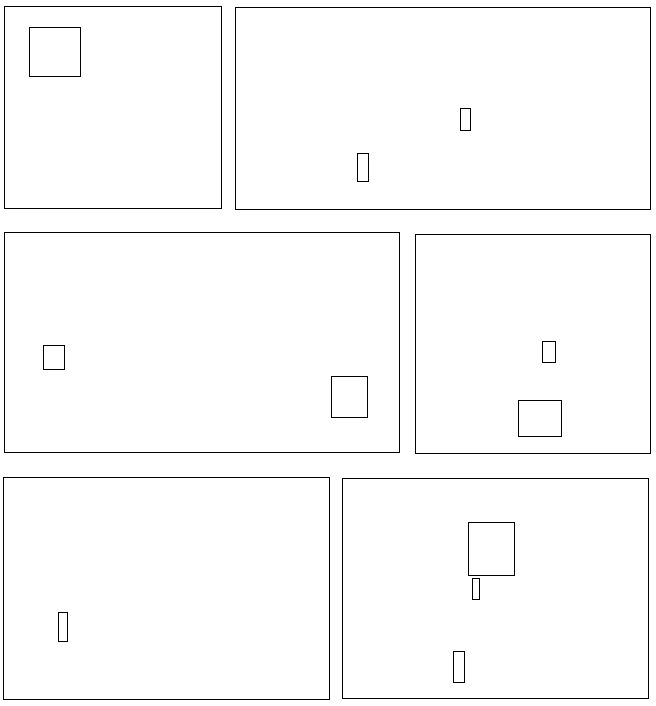
\includegraphics[trim= 1mm 0mm 0mm 0mm, clip, width=0.3\textwidth]{frame_unrecognized.png}}	\hspace{2em}
		\subfloat[Pruned panels]{\label{fig:se:frame_cleaned}
\includegraphics[trim= 1mm 0mm 0mm 0mm, clip, width=0.3\textwidth]{frame_cleaned.png}}
		  \caption[Topological pruning of panel bounding box extraction]{Topological pruning of panel bounding box extraction.}
		  %\label{fig:se:apl_1_0}
	\end{figure}
	%%%%%%%%%%%%%%%%%%%%%%%%%%%%%%%%%%%%%%%%%%%%%%%%%%%

Concerning the text cluster, we clearly see in figure~\ref{fig:se:frame_cleaned} that the spatial organisation is a characteristics of text regions (regardless of the language).
We group text candidates into text lines according to alignment and ignore text candidate that can not be part of any text line.

The gap between text (e.g. letter or attached letters, word) and text lines can vary significantly.
In fact, handwriting generates many artefacts such as lack of good alignment, mergers between letters and text lines.
We propose a method that handles the two first aforementioned artefacts considering only the height of the connected component.

We first search for the first letter (connected component) of each text line.
A letter is considered first if it is positioned on the left, on the same horizontal line and if there is no intersection found with any other letters at a distance equal to the letter height.
Then the other letters on the right are added by checking their relative horizontal and vertical positions.
For this purpose, we defined two conditions that are auto-adaptive to each letter (Figure~\ref{fig:se:letter_position}):

\begin{itemize}
    \item The horizontal inter-letter distance $d$ should be smaller than the maximal height of the letters ($d<Max(h1,h2)$);
    \item The vertical alignment is considered as correct if the vertical coordinate of the centre of the next letter $c2$ passes trough the first letter ($y_{min}(letter_1)>c2.y$ and $y_{max}(letter_1)>c2.y$);
\end{itemize}


	%%%%%%%%%%%%%%%%%%%%%%%%%%%%%%%%%%%%%%%%%%%%%%%%%%%
	\begin{figure}[h!]	%trim=l b r t  width=0.5\textwidth,
	  \centering
		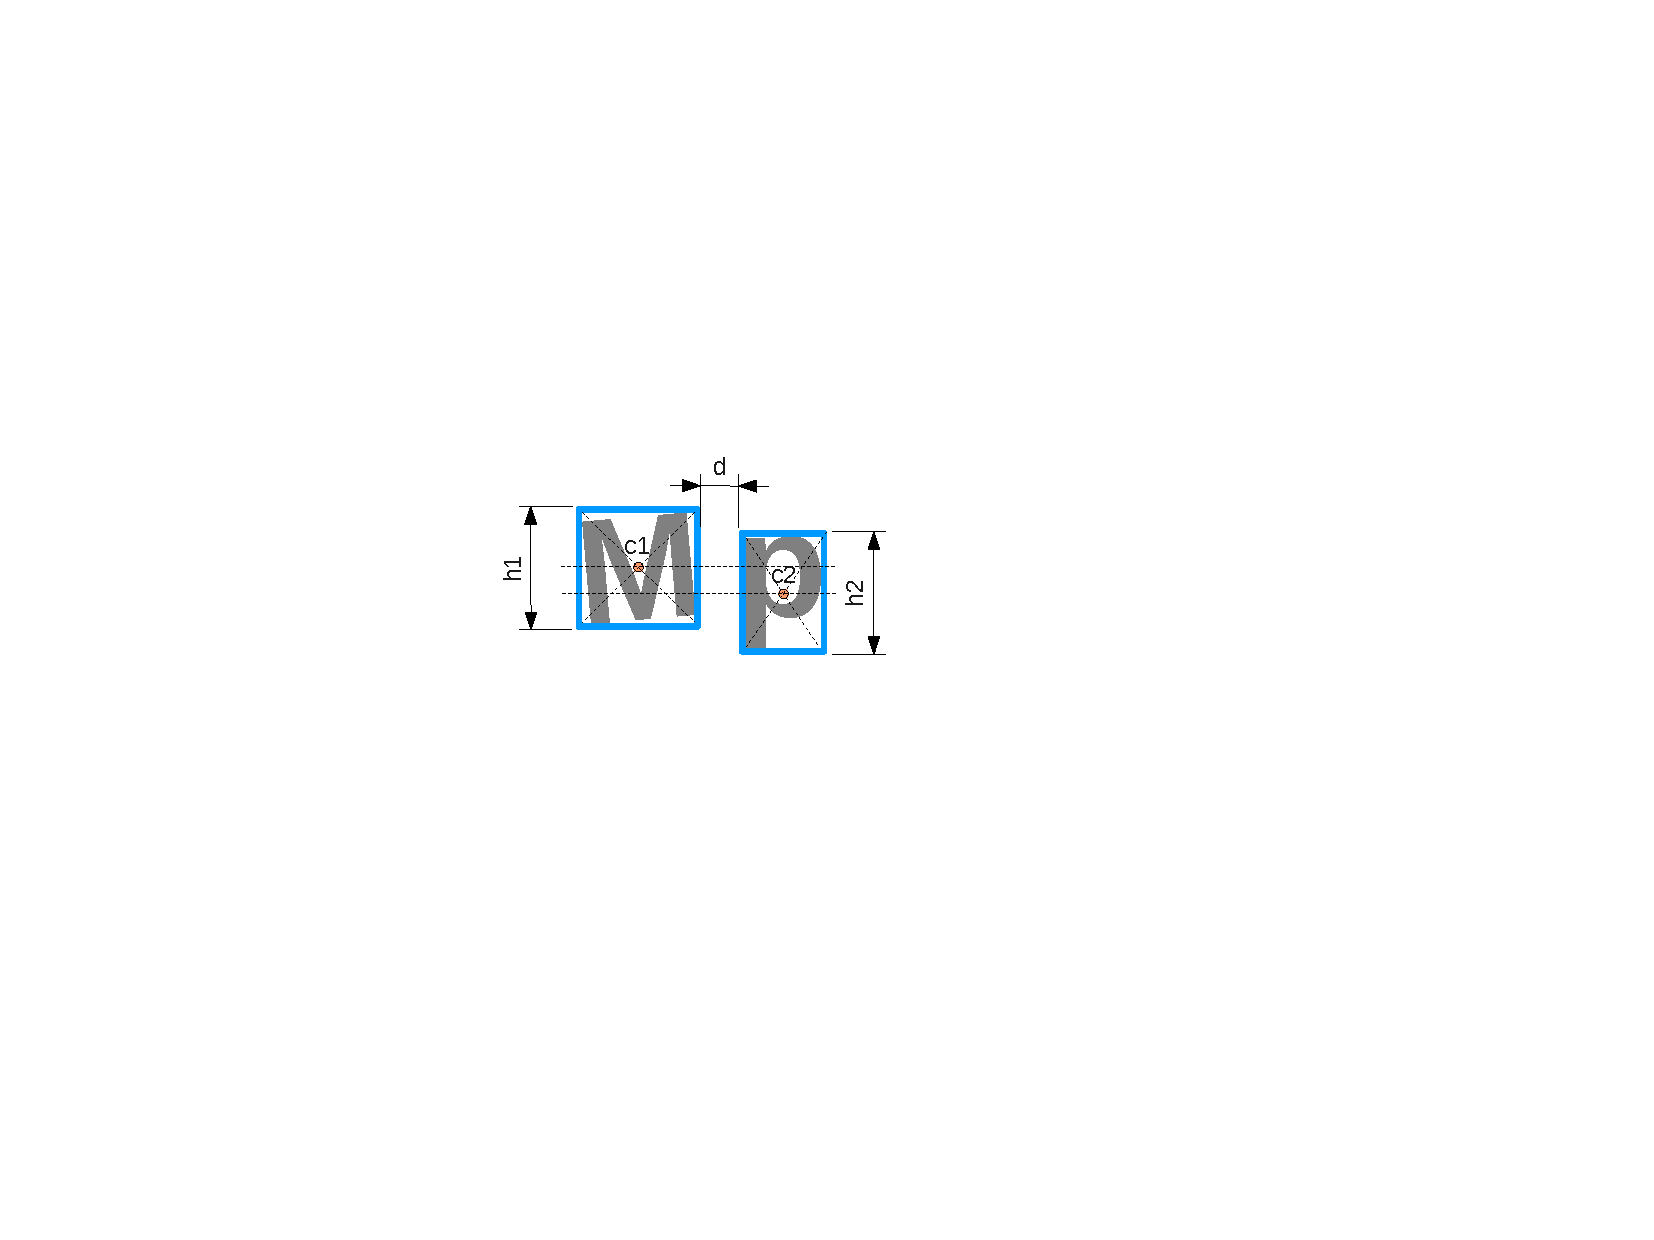
\includegraphics[trim= 200px 280px 300px 220px, clip, width=0.75\textwidth]{letter_position.pdf}
		\caption[Text letter horizontal and vertical alignments]{Letter horizontal and vertical positions variables (on the left $letter_1$, on the right $letter_2$). The two rectangles represent the bounding boxes and $c1$ and $c2$ their centres.}
		\label{fig:se:letter_position}
	\end{figure}
	%%%%%%%%%%%%%%%%%%%%%%%%%%%%%%%%%%%%%%%%%%%%%%%%%%%


 This is similar in principle to~\cite{Clavelli09} but adapted to take into account the horizontal alignment of text lines. Our method does not consider the letter width as we never know how many letters correspond to the CC.
 It can easily be used for vertical text by switching horizontal and vertical measurements.



	% paragraph pruning (end)

% paragraph classification (end)

% section panel_and_text (end)

\section{From text to balloon} % (fold)
\label{sec:se:from_text_to_balloon}
% In this section we detail a novel approach for closed and non-closed speech balloon localization in scanned comic book pages, an essential step towards a fully automatic comic book understanding. 
For comics content understanding, speech balloons present a lot of interest since they offer the links between the textual content and the comic characters providing information about the localization of the characters and the tone of speech. 
As mentioned in section~\ref{??}, speech balloons are the more frequent type of balloon in comics and are highly related to speech text regions.
In this section we propose two approaches form balloon extraction based on text region location that can be detected using the methods presented in section~\ref{sec:se:panel_and_text} or~\ref{sec:in:text_localisation_and_recognition}.
The first method defined as ``balloon'' the smallest connected-components contains several text regions.
The second method groups text lines into paragraphs and initializes an active contour model (snake) on its outline.
From the initial position, the snake is pushed away from the text and attracted by surrounding edges at the same time in order to stick to any potential balloon stroke close by.
The main advantage of the second method is its ability to detect implicit or partially drawn balloons as well as the closed ones.

\subsection{Regular balloon extraction} % (fold)
\label{sub:se:regular_balloon_extraction}
Regular balloon are defined as closed balloon with a completely drawn contour unlike implicit contour discussed in the next subsection~\ref{sub:implicit_balloon_extraction}.
Closed balloon are easily extractable using blob detection method similarly to the panel and text extraction presented above.
The main different lies in their dominant colour with is white and implies do extract white connected-components instead of black for panels and text.
One particularity of text inside balloons is its vertical and/or horizontal alignment in the balloon (Figure~\ref{fig:se:text_in_balloon}).
We propose to use this characteristic to compute a confidence value to each connected-component that include one or more text regions.

	%%%%%%%%%%%%%%%%%%%%%%%%%%%%%%%%%%%%%%%%%%%%%%%%%%%
	\begin{figure}[h!]	%trim=l b r t  width=0.5\textwidth,
	  \centering
		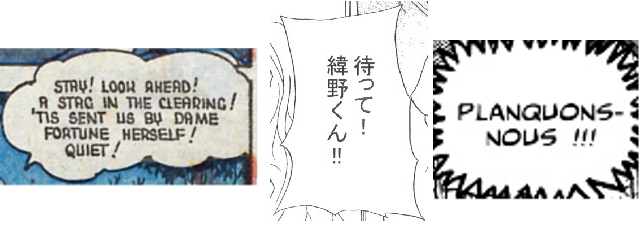
\includegraphics[trim= 0px 0px 0px 0px, clip, width=0.75\textwidth]{text_in_balloon.png}
		\caption[Text positions in speech balloons]{Example of text positions in speech balloons.}
		\label{fig:se:text_in_balloon}
	\end{figure}
	%%%%%%%%%%%%%%%%%%%%%%%%%%%%%%%%%%%%%%%%%%%%%%%%%%%

% The alignment confidence can be used in a later stage to classify balloon and non regions.
\paragraph{Blob extraction} % (fold)
\label{par:blob_extraction}

A typical ``closed'' balloon is surrounded by a black stroke that defined a white region (blob) inside it, with holes created by the presence of text letters.
We propose to make a binary segmentation of the comics image and then use connected-component labelling method to extract white blobs (Figure~\ref{fig:se:closed_balloon}).

	%%%%%%%%%%%%%%%%%%%%%%%%%%%%%%%%%%%%%%%%%%%%%%%%%%%
	\begin{figure}[h!]	%trim=l b r t  width=0.5\textwidth,
	  \centering
		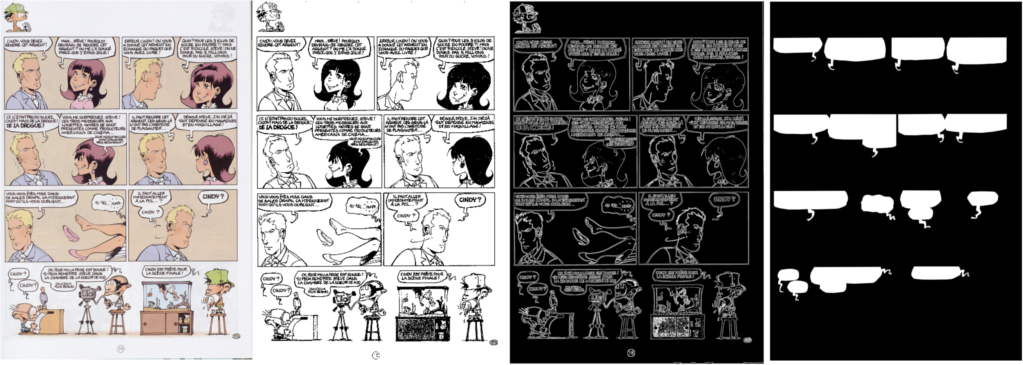
\includegraphics[trim= 0px 0px 0px 0px, clip, width=0.75\textwidth]{closed_balloon_process.png}
		\caption[Sequential balloon extraction process illustration]{Balloon extraction process. Original image, binary segmentation, contour detection (connected components) and result mask from left to right.}
		\label{fig:se:closed_balloon}
	\end{figure}
	%%%%%%%%%%%%%%%%%%%%%%%%%%%%%%%%%%%%%%%%%%%%%%%%%%%


% paragraph blob_extraction (end)

\paragraph{Text line grouping} % (fold)
\label{par:text_line_grouping}

As we are interested in localizing balloons from text, we post-process the results of the text line detection to group text lines into text area (paragraph), according to two rules.
First, we require that the candidate text lines to group have similar heights (or width in case of vertical text) and second that the inter-line distance is smaller than the average text line height of the potential paragraph region (Figure~\ref{fig:se:line_to_paragraphs}).

	%%%%%%%%%%%%%%%%%%%%%%%%%%%%%%%%%%%%%%%%%%%%%%%%%%%
	\begin{figure}[h!]	%trim=l b r t  width=0.5\textwidth,
	  \centering
		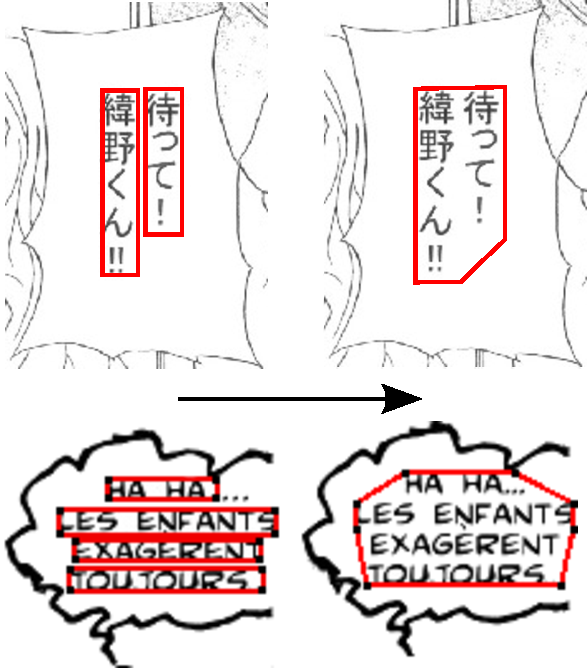
\includegraphics[trim= 0px 0px 0px 0px, clip, width=0.5\textwidth]{line_to_paragraphs.pdf}
		\caption[Text line to text paragraph conversion illustration]{Illustration of the text line to text paragraph conversion from left to right for vertical and horizontal text.}
		\label{fig:se:line_to_paragraphs}
	\end{figure}
	%%%%%%%%%%%%%%%%%%%%%%%%%%%%%%%%%%%%%%%%%%%%%%%%%%%

% paragraph text_line_grouping (end)

\paragraph{Balloon extraction} % (fold)
\label{par:balloon_extraction}

For each extracted blob that includes a text paragraph (one or more text lines), we compute the difference of alignment $C_{balloon}$ on the horizontal $d_x$ and the vertical $d_y$ axis between the balloon barycentre $c_1$ and the text paragraph barycentre $c_2$ (Figure~\ref{fig:se:align_diff}).

	%%%%%%%%%%%%%%%%%%%%%%%%%%%%%%%%%%%%%%%%%%%%%%%%%%%
	\begin{figure}[h!]	%trim=l b r t  width=0.5\textwidth,
	  \centering
		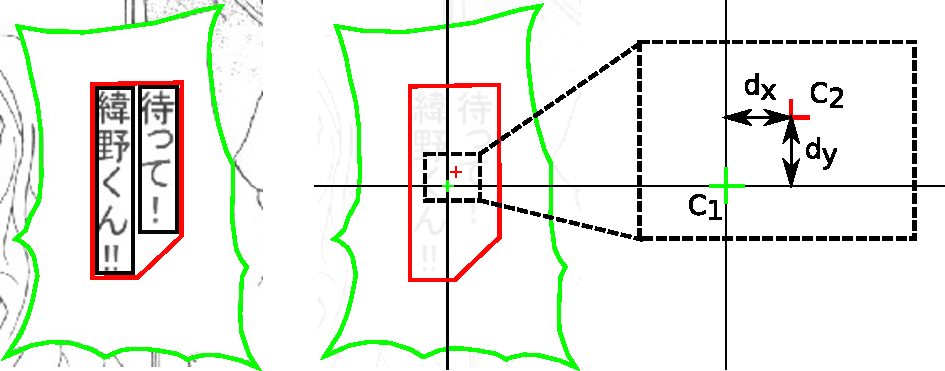
\includegraphics[trim= 140px 0px 0px 0px, clip, width=0.5\textwidth]{text_balloon_alignment.pdf}
		\caption[Illustration of the vertical and horizontal alignment differences between balloon and text region barycentre]{Vertical $d_y$ and horizontal $d_x$ alignment differences between balloon barycentre $c_1$ and text region barycentre $c_2$.}
		\label{fig:se:align_diff}
	\end{figure}
	%%%%%%%%%%%%%%%%%%%%%%%%%%%%%%%%%%%%%%%%%%%%%%%%%%%

Both differences $dx$ and $dy$ are normalized between zero and one as a percentage of the balloon width $B_{width}$ and height $B_{height}$ respectively.
The average of the vertical and horizontal alignments gives a confidence value for each balloon candidate, see formula~\ref{eq:se:balloon_confidence_value}.


\begin{equation}
	\label{eq:se:balloon_confidence_value}
	C_{balloon} = 1 - \frac{1}{2} *  \bigg( \frac{d_x}{B_{width}} + \frac{d_y}{B_{height}} \bigg)
\end{equation}

Balloon confidence value is used for balloon and non balloon classification in~\ch{chap:experimentations}.

% paragraph balloon_extraction (end)


% subsection regular_balloon_extraction (end)

\subsection{Implicit balloon extraction} % (fold)
\label{sub:implicit_balloon_extraction}

Balloon contour is not always completely drawn, it may be implied by contrast difference or other surrounding elements (Figure~\ref{fig:se:balloon_examples}c).
In most of the cases, including when contours are implicit, the location of text is generally a good clue to guess where the balloon is.
The problem of speech balloon outline detection can therefore be posed as the fitting of a closed contour around text areas, with the distinctiveness that the outline might not be explicitly defined in the image.
For the examples given in Figure~\ref{fig:se:balloon_examples}, this would be a smooth contour with relatively constant curvature (Figure~\ref{fig:se:balloon_examples}a), an irregular one with high local curvature (Figure~\ref{fig:se:balloon_examples}b), and an implicit one with missing parts (Figure~\ref{fig:se:balloon_examples}c).

	%%%%%%%%%%%%%%%%%%%%%%%%%%%%%%%%%%%%%%%%%%%%%%%%%%%
	\begin{figure}[!ht]%trim=l b r t  width=0.5\textwidth,
	\begin{center}
	  \begin{tabular}{ccc}
	  
\includegraphics[trim= 0px 2px 0mm 0mm, clip, width=0.13\textwidth]{round_balloon.png}&
	  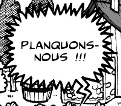
\includegraphics[trim= 0mm 0mm 0mm 0mm, clip, width=0.17\textwidth]{peaked_balloon.png}&
	  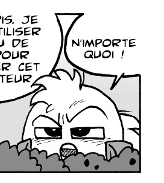
\includegraphics[trim= 15px 7mm 5px 0mm, clip, width=0.145\textwidth]{open_balloon.png} \\ 
	  \footnotesize a) Smooth	& \footnotesize b) Irregular & \footnotesize c) Implicit
	  \end{tabular}
	\caption[Speech balloon contour types]{Example of speech balloons with different contour types. Image credits~\cite{Bubble09}.}
	\label{fig:se:balloon_examples}
	\end{center}
	\end{figure}	
	%%%%%%%%%%%%%%%%%%%%%%%%%%%%%%%%%%%%%%%%%%%%%%%%%%%

Observing the heterogeneity of balloons, and considering the difficulty to manage ``open'' or ``implicit'' balloons, it appears necessary to use a dynamic and adaptive outline detection algorithm.
Active contours appear to be suitable to the problem.
The active contour framework was developed for delineating an object outline in an image.
The algorithm attempts to minimize the energy associated to the current contour, defined as the sum of an internal and an external energy term. 
In this paper we propose two adaptations of the active contour theory to the domain of comic balloon detection.
Specifically, we handle the case of balloons with missing parts or implicit contours, while we adopt a two-step approach to fit irregular outline types such as peak and cloud type balloons. 
To achieve this, we propose new energy terms making use of domain knowledge.


%------------------------------------------------------------------------
\subsubsection{Active contours}
\label{sec:se:active_contour}

The active contour~\cite{Kass1988} model is a deformable model, also known as snake, corresponding to a curve $\mathbf{v}(s)=[x(s),y(s)], s \in [0,1]$, that moves through the spatial domain of an image to minimize the energy functional (equation~\ref{eq:se:energy1}).

\begin{equation}\label{eq:se:energy1}
  E = \int_0^1 \! \frac{1}{2} \left( \alpha \left|\mathbf{v}'(s) \right|^2 + \beta \left| \mathbf{v}''(s) \right|^2 \right) + E_{ext}(\mathbf{v}(s))ds\\
\end{equation}
where $\alpha$ and $\beta$ are weighting parameters that respectively control the snake's tension and rigidity, and $\mathbf{v}'$ and $\mathbf{v}''$ denote the first and second derivatives of $\mathbf{v}(s)$ with respect to $s$. This functional energy is also called $E_{int}$ for internal energy.
The external energy function $E_{ext}$ is computed from the image so that it takes on its smaller values at the features of interest, such as boundaries~\cite{Xu1998}.
%It was initially designed to localize nearby edges accurately by using both internal and external energies (see eq.~\ref{eq:se:energy1}). 
%The external energy function $E_{ext}$ aim to attract the snake to the feature of interest (e.g. line, edge, corner), it is the image force. 
One of the proposed energy functions by Kass~\cite{Kass1988} is equation~\ref{eq:se:edge} which attracts the contour to edges with large image gradients. 
\begin{equation}\label{eq:se:edge}
  E_{ext} = -|\nabla \mathbf{I}(x,y)^2|
\end{equation}

We adapt the active contour framework to the domain of comics to detect speech balloons given a prior detection of text regions, introducing new energy terms based on domain knowledge about the relationship between text and balloons.
For the discussion below, we assume that text has been already detected in the image, see section~\ref{sec:se:panel_and_text} or~\ref{sec:in:text}.% and we use the method of \cite{Rigaud2013VISAPP} for text detection.

The introduction of statistical shape knowledge has already been studied in the literature~\cite{Cremers2002} but can not be applied here because of the lack of knowledge about the contour shape to detect.
Hence we introduce a new energy term, denoted $E_{text}$ (see equation~\ref{eq:se:energy2}) that conveys information about the relative placement of the balloon outline and the enclosed text.

\begin{equation}\label{eq:se:energy2}
  E = E_{int} + E_{ext} + E_{text}\\
\end{equation}

\subsubsection{External energy}
\label{sec:se:external_energie}
%The external energy $E_{ext}$ encourage curve onto image structures (e.g. edges, line, corner).

We consider edges as features of interest because we expect the speech balloon to be delimited by strong edges, at least partially.
Here we perform edge detection using the well know Sobel operator (Figure~\ref{fig:se:distance_transform}).
The original Kass~\cite{Kass1988} external energy (Equation~\ref{eq:se:edge}) is appropriate for natural scene images with smooth gradients but not for stroke-based images such as comics that comprise uniform coloured regions with strong edges.
In our case, we require that edges attract the snake from relatively far away (distances where the original edge gradient has already dropped to zero).
The method of Xu~\cite{Xu1998} would be appropriate here, although we have decided to use the equivalent distance transform of the edge image instead for computational efficiency reasons.
We therefore define the external energy function as:

\begin{equation}\label{eq:se:energy3}
  E_{ext} = \gamma \min A(i,j) = \gamma \min  \sqrt{(x_i-x_j)^2+(y_i-y_j)^2}\\
\end{equation}
where $E_{ext}$ is the minimum Euclidean distance ($A$) between a point $i$ and the nearest edge point $j$, $\gamma$ is a weighting parameter.

Since it is not desirable for edges corresponding to text to attract the snake, any edges that fall within the text regions are removed before the distance transform is calculated and do not contribute to the external energy.
	
	%%%%%%%%%%%%%%%%%%%%%%%%%%%%%%%%%%%%%%%%%%%%%%%%%%%
	\begin{figure}[!ht]	%trim=l b r t  width=0.5\textwidth,
	  \centering
		\fbox{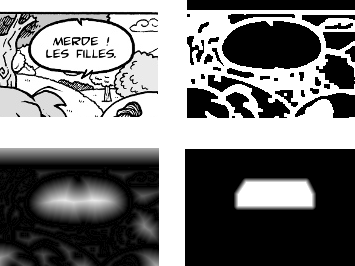
\includegraphics[trim = 0mm 0mm 7mm 0mm, clip, width=230px]{edge_dist_trans.png}}
		\caption[Active contour energies for open balloon extraction]{Example of original image (top left) and its corresponding non-text edge detection (top right), $E_{ext}$ energy (bottom-left) and $E_{text}$ energy (bottom-right). In the bottom part, white corresponds to high energy.}
		\label{fig:se:distance_transform}
	\end{figure}
	%%%%%%%%%%%%%%%%%%%%%%%%%%%%%%%%%%%%%%%%%%%%%%%%%%%

\subsubsection{Internal energy}
We use the original definition of the internal energy (see equation~\ref{eq:se:energy1}) which can by decomposed in two energy terms: $E_{cont} = \left|\mathbf{v}'(s) \right|^2$ and $E_{curv}=\left| \mathbf{v}''(s) \right|^2$.
%It is composed of a continuity and a curvature energies: $E_{internal} = \alpha E_{cont} + \beta E_{curv}$ as defined in eq.~\ref{eq:se:energy3}. The coefficients $\alpha$ and $\beta$ give more or less importance to one energy or another.
% 
% \begin{equation}\label{eq:se:energy3}
%   E_{internal} = \left( \alpha(s)  \left|\frac{d\bar{v}}{ds}(s) \right|^2 + \beta(s) \left| \frac{d^2\bar{v}}{ds^2}(s) \right|^2 \right) /2
% \end{equation}

The energy $E_{cont}$ forces the contour to be continuous by keeping points at equal distance, spreading them equally along the snake according to the average inter-point distance of the contour.
It becomes small when the distance between consecutive points is close to the average, see equation~\ref{eq:se:cont}.

\begin{equation}\label{eq:se:cont}
 E_{cont} = \alpha \Big|\bar{d} - \sqrt{(x_i - x_{i-1} )^2 + (y_i - y_{i-1} )^2}\Big|
\end{equation}
where $\bar{d}$ is the average distance between two consecutive points $i$ and $j$ of the snake and $\alpha$ is a weighting parameter.

The energy $E_{curv}$ enforces smoothness and avoids oscillations of the snake by penalizing high contour curvatures (minimizing the second derivative).
It becomes small when the angle between three points is close to zero, see equation~\ref{eq:se:curv}.
% Note, this energy itself makes the snake deflate and converge to a line or a point.

\begin{equation}\label{eq:se:curv}
  %E_{curv} = \beta | p_{i-1} - 2 * p_i + p_{i+1} |^2
  E_{curv} = \beta \left( (x_{i-1} - 2x_{i} + x_{i+1})^2 + (y_{i-1} - 2y_{i} + y_{i+1})^2 \right)
\end{equation}
where $i$ is a point of the snake and $\beta$ a weighting parameter.

%The distance $h1$ is an a priori distance between the text and its balloon. % for positioning the snake when there is a lake of external energy at low resolution detection.
%The distance $h2$ is the difference between the outer and the inner distance

\subsubsection{Text energy}
\label{sec:se:text_energie}

The text energy $E_{text}$ conveys domain specific knowledge about the relative locations of text areas and their associated balloon contours.
It is necessary in this domain to consider the lack of explicit information in the cases of implicit balloons, where parts of the outline are missing.
The $E_{text}$ energy aims at pushing the snake outwards toward the most likely balloon localization, given the position of the text area.
This energy term has two effects.
First, it acts collaboratively to the external energy, by moving the snake towards non-text edges (hopefully corresponding to the balloon outline).
Second, in the case of implied contours where no explicit edge exists (the external energy term is not informative), $E_{text}$ assists the algorithm to converge to an approximate contour position based on prior knowledge on the expected localization given the corresponding text area.
We define the text energy term at a localization $i$ of the image as follows:

\begin{equation}\label{eq:se:know}
E_{text} = \begin{cases} \kappa \frac{N}{min_{j \in T} A(i,j)} & \mbox{if } A(i,j) > 0 \\ \kappa N & \mbox{else} \end{cases}
\end{equation}
where $j$ is a pixel in the text area $T$, $N$ is an experimentally defined constant expressing the expected distance in pixel between the text area and the corresponding balloon boundary and $\kappa$ is a weighting parameter that controls the contribution of $E_{text}$ with respect to the other energy terms in eq.~\ref{eq:se:energy2}. Note when $i$ is on the border of $T$, the distance $A(i,j)$ is equal zero and the energy becomes maximal as if it was inside $T$.


\subsubsection{Proposed method}
\label{sec:proposed_method}

In this section we detail how to localize speech balloons using active contours based on the definitions given above. 
First we generate the static external energy map $E_{ext}$ for the whole image and then for each text area we compute the $E_{text}$ energy.
The internal energy $E_{int}$ is calculated for each point of the snake before each iteration.
We iteratively examine each point of the snake in a clockwise fashion and move it within a neighbourhood region of size $M$ in order to minimize equation~\ref{eq:se:energy2}.
This operation is repeated until no point moves in one turn (see algorithm~\ref{al:be:method}).
We perform a first smooth-contour approximation of the balloon boundary (low resolution) and then we fit the contour better to the balloon shape (high resolution) using the same algorithm

TODO: remove high resolution step???
%, especially for non-smooth boundaries.% High resolution contour shape fitting - aiming to 
 %\item Contour classification [NOVELTY? SHAPE COMPOSED BY DIFFERENT PART OF SHAPE]

\begin{algorithm}
\caption{Open balloon detection loop}
\label{al:be:method}
\begin{algorithmic}
%\REQUIRE $n \geq 0 \vee x \neq 0$
%\ENSURE $y = x^n$
%\STATE $y \leftarrow 1$
\STATE{compute $E_{ext}$ energy}
\FOR{each text area}
  \STATE compute $E_{text}$ energy
  \STATE active contour initialization
  \STATE stop = False
  \WHILE{stop = False}%\STATE{DO}
    \STATE $n = 0$
    \FOR{each points of the snake}
      \STATE examine neighbourhood position energies
      \IF{one position reduce the current energy}
		\STATE move point to this position
		\STATE $n=n+1$
      \ENDIF
    \ENDFOR
    % \STATE // If not points have been moved then stop
    \IF{$n = 0$}
    	\STATE{stop = True}
    \ENDIF
  \ENDWHILE% <--- use \doWhile for the "while" at the end %\While{$n > 0$}
\ENDFOR
\end{algorithmic}
\end{algorithm}

\subsubsection{Active contour initialisation}
\label{sec:se:cont_init}

The active contour is initialized on the outline of the text paragraph region.
This corresponds to the convex hull of all the text lines that are included in the balloon (Figure~\ref{fig:se:paragraphs}b).
Note that the convex hull of the text area also corresponds to the $E_{text}$ maximal value border (Figure~\ref{fig:se:distance_transform}).
%At this point, the $E_{text}$ has to be the strongest in eq.~\ref{eq:se:energy2} in order to ``push'' away the snake from the text area and then facilitate its attraction by $E_{ext}$ (non text edges).
%Another possible initialization strategy could be to use the smaller ellipse circumscribing the text area.% This has been experimented section~\ref{sec:experiments}.

%Note, in case of wrong initialization, the external energy allow the snake to inflate deflate in the case of the snake initialization is outside the balloon. Gradients that are inside the initial curve repulsed the contour (considered as text areas).


%\subsubsection{Number of points}
The initial number of points impacts the way that the snake moves and the precision of the final detection.
During the first low resolution localization step, we perform a spaced equipartition of the points (Figure~\ref{fig:se:paragraphs}c) to quickly localize the global shape avoiding unnecessary stops on image details.
In the subsequent high resolution fitting stage, we add more intermediate points to fit the exact shape more precisely.
% with an inter-points distance fixed to half line height

%%%%%%%%%%%%%%%%%%%%%%%%%%%%%%%%%%%%%%%%%%%%%%%%%%%
	\begin{figure}[!ht]%trim=l b r t  width=0.5\textwidth,
	\begin{center}
	  \begin{tabular}{ccc}
	  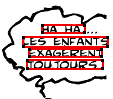
\includegraphics[trim= 0mm 0mm 0mm 0mm, clip, width=0.20\textwidth]{group_lines.png}&
	  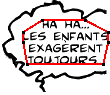
\includegraphics[trim= 0mm 0mm 0mm 0mm, clip, width=0.20\textwidth]{convex_hull.png}&
	  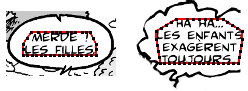
\includegraphics[trim= 48mm 0mm 0mm 0mm, clip, width=0.20\textwidth]{snake_init.png} \\ 
	  \footnotesize a) Group of text lines	& \footnotesize b) Text area convex hull 	& \footnotesize c) Snake initialization 
	  \end{tabular}
	\caption[Active contour initialization based on text region convex hull]{Active contour initialization based on text region convex hull.}
		\label{fig:se:paragraphs}
	\end{center}
	\end{figure}	
	%%%%%%%%%%%%%%%%%%%%%%%%%%%%%%%%%%%%%%%%%%%%%%%%%%%


%We initialize the active contour of $N$ points on the paragraph shape (group of lines) figure~\ref{fig:se:paragraphs} and then we make it grow until it hits edges.
%We define a paragraph as a group of text lines spoken by the same speaker and with no interruptions (e.g. time break, interaction, other person talk). These group of lines are written close to each other by convention . We labelize two consecutive lines as part of the same paragraph if there is no enough space for an other line similar in height between them.

\subsubsection{Low resolution contour localization}
Following a two stage process, we first aim to obtain a rough localization of the balloons by fitting a smooth contour using a few contour points during initialization.
The idea is to progressively push the snake away from the text area and towards the balloon boundary giving an increased weight to both the $E_{ext}$ and $E_{text}$ energy terms.
If the balloon has an explicit boundary then $E_{ext}$ will attract the snake to it.
If there is no explicit contour close enough to attract the snake then the $E_{text}$ term will push the snake to the suggested position of the balloon contour.
Also the internal energies are important at this stage to maintain a certain rigidity of the snake.
%The and low external energy parameter $\gamma$, a large internal curvature energy parameter $\beta$ and a large knowledge energy parameter $\eta$ (Fig.~\ref{fig:se:multiscale01}). 
At the end of this step, we obtain a preliminary localization of the speech balloons (Figure~\ref{fig:se:mono_res_det}). 

	%%%%%%%%%%%%%%%%%%%%%%%%%%%%%%%%%%%%%%%%%%%%%%%%%%%
	\begin{figure}[!ht]	%trim=l b r t  width=0.5\textwidth,
	  \centering
		% \fbox{
		
\includegraphics[trim = 0mm 3mm 0mm 1mm, clip, width=220px]{mono_res_det.png}
		% }
		\caption[Examples of low resolution contour detection for balloon extraction]{Example of low resolution contour detection (red line) for irregular closed (left) and smooth open (right) balloons.}
		\label{fig:se:mono_res_det}
	\end{figure}
	%%%%%%%%%%%%%%%%%%%%%%%%%%%%%%%%%%%%%%%%%%%%%%%%%%%

% \subsection{Candidate point selection}
% {\bf SECTION REMOVED because we don't know yet how to efficiently select the point and because multi-resolution method already improves results without using candidate point selection. We can mention it in the prospects.}

%The candidate point selection aim to determine if the snake segments between points can be more detailed or not (e.g. detection of peak, circle, tail). Figure~\ref{fig:se:multiscale01} shown two categories of points, those who has been attracted and stopped by edge (part of the real contour) and the others (part of the suggested contour). At this point we can see that adding more points on the real contour parts and relaxing the internal energies could improve the contour detection. This a true but then all the contour will be affected and we could degrade the suggested contour detection part if it is a non closed contour. Therefore we add new points only between those stopped by edge because we can not get more detail about suggested parts of the contour and we could even loose the low resolution detection information.
%We consider as ``stopped'' the points that are common with the ``text less'' edge map (left part of fig.~\ref{fig:se:distance_transform}).
 %An example of candidate points is on figure~\ref{fig:se:multiscale01} and~\ref{fig:se:multiscale02}). We keep those new generated points only if they hit and edge before the snake stabilize again (only if they improve the contour detection). The aim is to get a higher resolution contour detection only where there is a contour drawn. If no contour (non closed balloon case) then we keep the appropriate shape from low resolution detection.


\subsubsection{High resolution contour shape fitting}
Figure~\ref{fig:se:mono_res_det} shows that the global shape of the top balloon has been detected although it is still far from a perfect fit because, as we can see on bottom part of the balloon, the snake was not able to fit precisely balloon outline, for instance peaky and tail regions are not well segmented.
To achieve a better fitting, we increase the resolution of the snake by adding new points between the current ones and by changing the weighting parameters of the energy function, and go through a second fitting process.
At this stage, we relax the $E_{curv}$ energy to make the snake to thinner parts of the boundary and we set $E_{cont}$ strong enough to keep a regular inter-point distance all over the contour.
Also, we reduce the $E_{text}$ energy weight because at this step, the snake is already far from text and this term is not informative any more.
%to give more importance to the image energy than the prior knowledge. %is reduced because  external  avoid point  is closer to the final contour and do not need the $E_{know}$ energy start to minimize we reduced the inter-points distance, we also increase the external energy parameter $\gamma$ to make the snake more attractable by image edge, decrease the internal curvature energy parameter $\beta$ to allow more flexible contour fitting and decrease the knowledge energy parameter $\eta$ because the contour is now far from the text. 
This new configuration allows the snake to fit more precisely to the balloon contour as shown in figure~\ref{fig:se:hd_contour} (to compare with figure~\ref{fig:se:mono_res_det}).

%{\bf TO ADD IF RESULTS CONFIRMS: we consider external energy map based from edge detection only (no distance transform any more)?}

	%%%%%%%%%%%%%%%%%%%%%%%%%%%%%%%%%%%%%%%%%%%%%%%%%%%
	\begin{figure}[!ht]	%trim=l b r t  width=0.5\textwidth,
	  \centering
		\fbox{
\includegraphics[trim = 0mm 2mm 0mm 1mm, clip, width=180px]{multi_res_det.png}}
		\caption[Examples of high resolution contour detection for balloon extraction]{Examples of high resolution contour detection (red line) for closed (left) and open (right) balloons.}
		\label{fig:se:hd_contour}
	\end{figure}
	%%%%%%%%%%%%%%%%%%%%%%%%%%%%%%%%%%%%%%%%%%%%%%%%%%%

% subsection implicit_balloon_extraction (end)

% section from_text_to_balloon_ (end)

\section{From balloon to tail} % (fold)
\label{sec:se:from_balloon_to_tail}

Speech balloons indicate dialogue with tails pointing at their respective speakers~\cite{Varnum2007Language}
%Balloon tails tell the reader the relationships between a set of textual or graphic elements contained in the speech balloons and the comics characters [REF???].
, usually represented by a discontinuity on balloon contour (Figure~\ref{fig:se:tail_types}). 
We propose to detect the tail position and direction based on the balloon contour analysis.
We limit this study to the tail types that can be considered has an extension of the inside region (background) of the speech balloon namely types ``comma'', ``zigzag'' and ``absent'' in Figure~\ref{fig:se:tail_types} because they can all be extracted from the segmentation of the balloon background.
Other types require a specific study from the speech balloon extraction that should consider the contour stroke and surrounding elements.

    %%%%%%%%%%%%%%%%%%%%%%%%%%%%%%%%%%%%%%%%%%%%%%%%%%%%%%%%
    \begin{figure}[ht]%trim=l b r t  width=0.5\textwidth,  
      \centering
      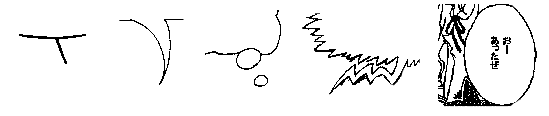
\includegraphics[trim= 0px 0px 0mm 0mm, clip, width=0.75\textwidth]{tail_types.png}
    \caption[Examples of type of speech balloon tails]{Examples of type of speech balloon tails. From left to right: stroke, comma, circle, zigzag, absent.}
    \label{fig:se:tail_types}
    \end{figure}
    %%%%%%%%%%%%%%%%%%%%%%%%%%%%%%%%%%%%%%%%%%%%%%%%%%%%%%%%

We propose a method to describe ``comma'', ``zigzag'' and ``absent'' (no tail) types.
The tail can be decomposed into four elements: origin, path, tip and pointed direction.
The contour of a speech balloon is mainly convex except in the region where the tail is connected to the balloon (origin) which produces the highest convexity defects.
If the speech balloon has no tail, there is no particular convexity defect.
% and we can also detect it, see the end of this subsection.
%We propose to detect the two biggest convexity defects to locate the tail origin.
A convexity defect is defined by a triangle from one segment of the balloon convex hull to the farthest point on the balloon contour (Figure~\ref{fig:se:convexity_defects}).
The set $F=\{f_0,f_1,...f_n\}$ represents farthest points from the corresponding hull segments $S=\{s_0, s_1,...,s_n\}$ where $n$ is the number of hull segments.
We define the top two farthest points $f_a$ and $f_b$ corresponding to the convex hull segments $s_a$ and $s_b$, as the coordinates of the tail origin (Figure~\ref{fig:se:convexity_defects}).

    %%%%%%%%%%%%%%%%%%%%%%%%%%%%%%%%%%%%%%%%%%%%%%%%%%%%%%%%
    \begin{figure}[ht]%trim=l b r t  width=0.5\textwidth,  
      \centering
      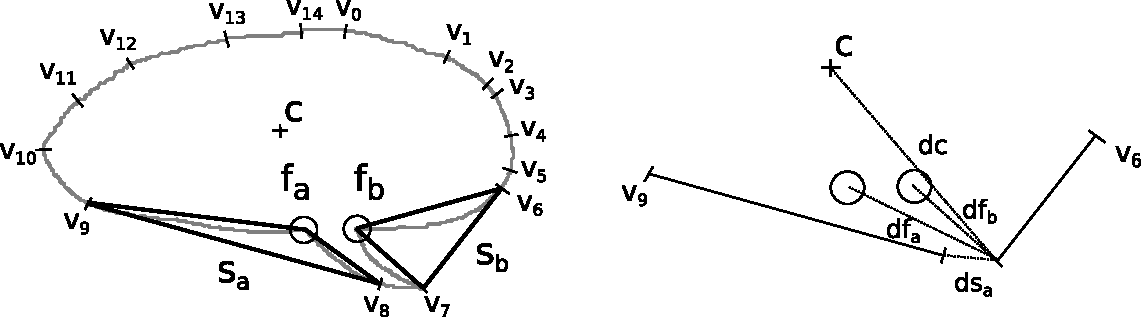
\includegraphics[width=0.9\textwidth]{tail_description.pdf}
    \caption[Representation of the two biggest convexity defects that defines the tail origin]{Representation of the two biggest convexity defects that defines the tail origin $f_a$ and $f_b$ (left). On the right side, we represent the distances related to the vertex $v_7$ to illustrate the variables of equation~\ref{eq:se:optimisation}. In this case $ds_b=0$ because $v_7$ coincides with an end of segment $s_b$ (distance equal to zero).}
    \label{fig:se:convexity_defects}
    \end{figure}
    %%%%%%%%%%%%%%%%%%%%%%%%%%%%%%%%%%%%%%%%%%%%%%%%%%%%%%%%

Most of the time, the tail tip corresponds to one of the vertices of the convex hull.
We define the set of vertices $V=\{v_1,v_2,...,$ $v_n\}$.
The optimal vertex is computed by comparing five features that corresponds to the Euclidean distances:

\begin{itemize}
   \item $ds_a$ the distance to the segment $s_a$
   \item $ds_b$ the distance to the segment $s_b$
   \item $dc$ the distance to the centre of mass $c$ of the balloon
   \item $df_a$ the distance to the tail origin $f_a$
   \item $df_b$ the distance to the tail origin $f_b$
 \end{itemize} 

This can be formulated as:
\begin{equation}\label{eq:se:optimisation}
   v* = argmax\big( max(dc+df_a+df_b) + min(ds_a + ds_b) \big)\\
 \end{equation}
 where $v*$ is the optimal vertex from the set of vertex $V$.
%NEW IDEA: for all the vertex between the two defects, min/max a feature vector (dist to barycentre, distance to tail origin).
% Most of the time both triangles intersect on the same point which is the tail tip $T$.
% If not, we determine which pair of points from the two segments that are the closest ($t_1$ and $t_2$) and then which one is the tail tip ($t_1$ or $t_2$).
% The tail tip is defined by the farthest from the tail origin:
% $T = \begin{cases} t_1, & \mbox{if } dist(f_1,t_1) > dist(f_2,t_2) \\ t_2, & \mbox{else} \end{cases}$
%Each segment of the convect hull has a convexity defect that we $cd_i$ 

Together with the position, we compute a confidence value $C_{tail}$ related to the mean depth of $f_a$ and $f_b$ over the mean balloon size $meanBalloonSize$, see formula~\ref{eq:se:confidence_tail}.

\begin{equation}
\label{eq:se:confidence_tail}
  C_{tail} = \frac{(depth(f_a)+depth(f_b))/2}{meanBalloonSize}
\end{equation}
where $depth(f_x)$ is the depth of the corresponding defect in number of pixels and $meanBalloonSize$ is defined in equation~\ref{eq:se:mean_balloon_size}.


\begin{equation}
  \label{eq:se:mean_balloon_size}
  meanBalloonSize = \frac{\sum\limits_{i=0}^n Wb_i + \sum\limits_{i=0}^n Hb_i}{n * 2}  
\end{equation}
where $Wb_i$ and $Hb_i$ correspond to the width and the height of a speech  balloon $i$ and $n$ the number of speech balloons in the image.

% By measuring the variance in of all the convexity defect distances $\sum\limits_{i=0}^n var(f_i)$ of the contour we can detect if there is a tail or not, see equation~\ref{eq:se:var_defects}.
% We use a fixed threshold of $thV=10\%$ of the balloon height to decide if a balloon has a tail or not, see equation~\ref{eq:se:var_defects}.

% \begin{equation}
% \label{eq:se:var_defects}
%   hasTail = \begin{cases} 1, & \mbox{ if } \sum\limits_{i=0}^n var(f_i) > thV \\ 0, & \mbox{ else}  \end{cases}
% \end{equation}
% where $thV$ is a decision threshold relative to the average balloon size in the image.

Once we find the tail tip, we analyse its neighbourhood to find the orientation and the direction of the last part of the tail which is directed towards the speaking character.
We compute a $M$x$M$ square region centred on the tail tip position in the balloon mask and use a line fitting algorithm (weighted least-squares) that returns the representative line that minimizes the distance between all the points of the local region (Figure~\ref{fig:se:orientation}).


    %%%%%%%%%%%%%%%%%%%%%%%%%%%%%%%%%%%%%%%%%%%%%%%%%%%%%%%%
    \begin{figure}[ht]%trim=l b r t  width=0.5\textwidth,  
      \centering
      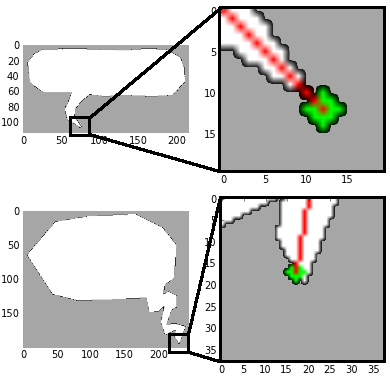
\includegraphics[width=0.5\textwidth]{tail_direction.png}
    \caption[Tail orientation given by the line fitting algorithm in the neighbourhood of the tail tip]{Tail orientation given by the line fitting algorithm in the neighbourhood of the tail tip.}
    \label{fig:se:orientation}
    \end{figure}  
    %%%%%%%%%%%%%%%%%%%%%%%%%%%%%%%%%%%%%%%%%%%%%%%%%%%%%%%%


The tail direction is computed from the tail orientation that has initially two possible directions.
We define the tail direction from the closest point $fitLinePoint$ of the representative line to the tail origin, to the tail tip ($vec\{fitLinePoint,$ $tailTip\}$).
 %by selecting the vector that starts close to the $F$ points and ends far from the $F$ points:

%$\dot{\vec{p}} = m\vec{v}$
% $\vec{vec\{dir\}} = \begin{cases} vec\{x_1,x_2\}, & \mbox{if } d(f_1,x_1) + d(f_2,x_1) < d(f_1,x_2) + d(f_2,x_2) \\ vec\{x_2,x_1\}, & \mbox{else} \end{cases}$

% section from_balloon_to_tail (end)


%--------------------------------------------------------------------------------------------------------------------------------------
\section{From tail to comic character} % (fold)
\label{sec:se:tail_to_character}


%from_tail_to_comic_character detecting the characters, in their great diversity, from the drawings of a comic book's page is quite a piece of work, 
% To detect comic characters from the tail detection, we narrow down the panel region according to position of the tail tip and to direction it is pointed to.
% area where we are going to look for them in.
% This can be done thanks to the panel, balloon and tail detection we extracted on the image during the previous steps.
% We make the assumption that the main characters of a story speak at some point.
% We focus on the characters that are emitting a speech balloon (speaking characters) and try to localize them from the speech balloon informations.
% That is to say that speech balloons will be associated one or several times to each of the character in different panels.

As we know which balloons are in which panel (total inclusion), we can estimate from the position and direction of the tail, which part of the panel may contain the speaking character.
The tail orientation is quantized in eight cones of $\pi/4$ radius so we can consider that, in a rectangular-shaped panel (or its bounding box), the tail is either pointing towards a corner or towards a border of the panel.
We define the ROI for the character as a squared region beside the speech balloon.
The maximum width $w_{max}$ and height $h_{max}$ of the ROI are equal to the mean widths and heights of all the balloons in the image, see equation \ref{eq:se:mean_balloon_size}.

The position of the ROI around the speech balloon is defined by two opposite points of a square $A_{x,y}$ and $B_{x,y}$ according to formula~\ref{eq:se:roi_position_around_balloon} which is sometimes constrained by a panel border that is why the term $min()$ appears.
The different positions of the ROI are illustrated on figure \ref{fig:se:roi_area}.

\begin{equation}
  \label{eq:se:roi_position_around_balloon}
  \begin{array}{rccl} 
	  A_x & = & v^*_x - min(Pi_x - v^*_x, w_{max}) & * O_x \\ 
	  A_y & = & v^*_y - min(Pi_y - v^*_y, h_{max}) & * O_y \\ 
	  B_x & = & \left[ A_x + min(Pi_x - A_x, w_{max}) \right] & * O_x \\ 
	  B_y & = & \left[ A_y + min(Pi_y - A_y, h_{max}) \right] & * O_y
  \end{array} 
\end{equation}
where $v^*$ is the coordinates of the tail tip (see section~\ref{sec:tail_extraction}), $Pi$ the coordinates of one of the four corners of the panel bounding box $P=\{P0, P1, P2, P3\}$ and $O$ the offset for the direction of the tail.
The offset $O$ is quantized in heigh values according to the tail direction and the panel's corner $P_i$ is chosen accordingly, see table~\ref{tab:se:offset_panel_corner}.

    %%%%%%%%%%%%%%%%%%%%%%%%%%%%%%%%%%%%%%%%%%%%%%%%%%%
  \begin{table}[ht]
    \normalsize
%\renewcommand{\arraystretch}{1.2}

    \centering
    \caption{Values of the offset $O$ on horizontal and vertical axis and panel's corner selection according to the eight directions of the tail.}
    % \def\arraystretch{1.5}%  1 is the default, change whatever you need
    \setlength{\tabcolsep}{.45em}
    % \extracolsep{\fill}
    \begin{tabular}{|c|c|c|c|c|c|c|c|c|}

          \hline
	      &  N  & NE  & E  & SE & S & SW & W & NW   \\
	      \hline
	      $O_x$   & 0.5  & 0.75 & 1.0  & 0.75 & 0.5 & -0.75& -0.5 & 0.75  \\
	      \hline
	      $O_y$   & -1   & -0.75& -0.5 & 0.75 & 1.0 & 0.75 & -0.5 & -0.75  \\
	      \hline
	      $Pi$    & P1   & P1   & P1   & P1   & P3  & P3   & P3   & P3   \\
          \hline
        \end{tabular}
    \label{tab:se:offset_panel_corner}
  \end{table}%
    %%%%%%%%%%%%%%%%%%%%%%%%%%%%%%%%%%%%%%%%%%%%%%%%%%%


% Sometimes the pointed corner or border is far from the tail tip and create a wide region.

%An analysis of the eBDtheque ground truth gave us the confirmation that this estimated areas were actually containing more than 70\% of the characters with a precision of 50\% in average.

%%%%%%%%%%%%%%%%%%%%%%%%%%%%%%%%%%%%%%%%%%%%%%%%%%%
 \begin{figure}[!ht]
   \centering
  %\includegraphics[width=150px]{fig/roi_area.pdf}
  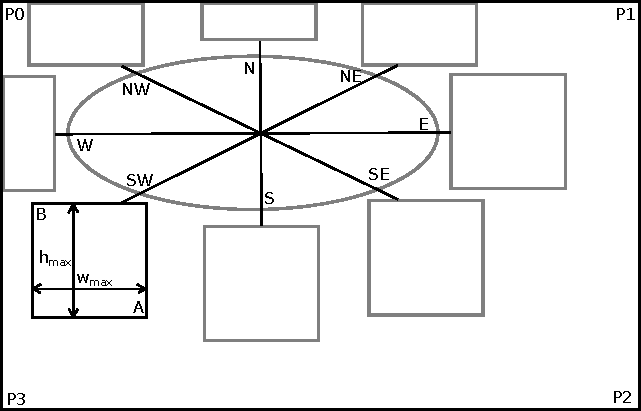
\includegraphics[width=180px]{roi_hypothesis.pdf}
  \caption[Illustration of the character region of interested computation for each of the eight directions of the tail]{Illustration of a panel with four corners $P0, P1, P2, P3$ and the different ROI position and size that can be defined for each of the eight directions of the tail.
  }
  \label{fig:se:roi_area}
 \end{figure}
%%%%%%%%%%%%%%%%%%%%%%%%%%%%%%%%%%%%%%%%%%%%%%%%%%%

% The ROI are then passed to the comic character extractor (see section~\ref{sub:character_extraction}) which will locate more precisely the characters based on image features.
% image processing part (character extractor) that will spot all the characters, especially the ones that does not speak, using those regions as seeds.


% section from_tail_to_comic_character (end)

% Conclusion --------------------------------------------------------------------------------------------------------------------------------------
\section{Conclusions}
\label{sec:se:conclusion}
In this section we have presented how to understand comics image content by following the relations between elements, defined by knowledge domain.
This approach is quite natural, trying to reproduce the reader's reading behaviour: first to search for the panels and then speech balloons, read their content and make the link with the characters and other graphic in the panel.
Despite the intuitiveness of this approach, the main drawback of this sequential approach is the dependency of the processes which propagates errors.
The experiments section~\ref{sub:ex:sequential_information_extraction_evaluation} evaluates the processes that are proposed here.

% In this section we have presented and evaluated two methods for panel extraction based on connected-components labelling.
% The experiments shows that both approaches are really efficient for comics using gutter where there is no drawing between panels.
% The first method have been published for national and international audience~\cite{rigaud2012extraction,Rigaud2012LNCS} and the second method is part of an international journal publication [pending acceptance???].

% Then, the variance of each class is computed to check the homogeneity of the ROI. If the variance of the ``frame'' class is high, a specific algorithm~\cite{Khoi11} is applied in order to improve the previous steps (binarisation and/or classification). 

Next chapter is going to present a non sequential approach able to extract comics image content using independent processing in order to avoid error propagation.

% Also, an open balloon detection method based on speech text position will be presented.


% \begin{itemize}
% 	% \item Compute a confidence value between 0 and 1 for each panel: the inverse of overlapping percentage with other panels. (maximal when no overlap). This can replace the topological filtering by considering as correct the panel with a confidence > 0\%
% 	\item \url{/PhD/publication/2013/LNCS/robust_frame_and_text_extraction_from_comic_books/paper}
% 	\item IJDAR paper > panel extraction %\url{/PhD/Publications/CIFED_2012}
% \end{itemize}

\chapter{Method 2: independent information extraction}
\chaptermark{Independent information extraction}
\label{chap:independent}
\graphicspath{{./chapters/4-independent/figs/}}

%Abstract-------------------------------------------------------------------------------------------------------------
%In this chapter we propose a symbol spotting technique in graphical documents. Graphs are used to represent the documents and an error tolerant (sub)graph matching technique is used to detect the symbols in them. We propose a graph serialization to reduce the usual computational complexity of graph matching. Serialization of graphs is performed by computing acyclic graph paths between each pair of connected nodes. Graph paths are one dimensional structures of graphs, handling which is less expensive in terms of computation. At the same time they enable robust localization even in the presence of noise and distortion. Indexing in large graph databases involves a computational burden as well. We utilize a graph factorization approach to tackle this problem. Factorization is intended to create a unified indexed structure over the database of graphical documents. Once graph paths are extracted, the entire database of graphical documents is indexed in hash tables by locality sensitive hashing (LSH) of shape descriptors of the paths. The hashing data structure aims to execute an approximate $k$-NN search in a sub-linear time. We have performed detailed experiments with various datasets of line drawings and the results demonstrate the effectiveness and efficiency of our technique.
%----------------------------------------------------------------------------------------------------------------------

In this chapter we propose an independent extraction of each element contained by comic book images.
This content retrieval approach tries to fill the weaknesses of the sequential approach presented in the previous chapter.
New approaches for extracting panels, text, balloons and comic characters are presented successively but they can be used in any order as they are completely independent for each other.
New domain knowledge are embedded in the low level processing to process each image in and autonomous way with a similar performance.


\section{Introduction}
\label{sec:in:intro}

\modif{TODO or REMOVE}

\section{Panel extraction}
\label{sec:in:panel_extraction}

The previous clustering-based method presented in Section~\ref{sec:se:panel_and_text} is particularly useful for simultaneous extractions, as illustrated panel and text while removing noise region at the same time.
Nevertheless, the panel extraction can be improved if we focus on panel elements only.
We propose to use a second characteristic of panels which is their topological relations with other elements in the image.
Figure~\ref{fig:se:cc_bounding_box} shows that outermost or external contours actually corresponds to panels.
We base this method on this criterion, considering the panels to be the outermost contours.
This is especially true for general comics using gutter (white space) between panels.
Making the outermost contour as panel can be seen as a binary classification method deriving from a more generic concept.
The general concept would attribute a confidence value to each contour in the image, inversely promotional to their percentage of inclusion in other contours.
Non included contour (outermost) would have the maximum confidence and fully included ones the lowest confidence in being a panel.

% We propose to combine the advantages of the already published panel extraction methods~\cite{Arai11,Rigaud2012LNCS} and partially solve their weaknesses using the expert system model.
% that we present section~\ref{sec:expert_system}.
% They are connected component based methods that are reliable for comics with disconnected panels (separated by gutters).
% no gutter between the panels (they are separated by a single black line).
% Line-based decomposition methods are the efficient methods for line separated comics~\cite{Li2013Unsupervised} (no gutter).
% A generic method that works best with both styles is not obvious.
% We combine~\cite{Arai11,Rigaud2012LNCS} to introduce a new method, especially suitable for general comics using gutter (white space) between panels.

Panel contours (border line) are usually dark and similar for all the panels of a comics page.
Sometimes panel contours are implicit as shown Figure~\ref{fig:in:se:panel_img} (considered as a difficult case).
In this case, the reader distinguishes them by comparing the difference of colour between the panel content and the page background.
We use a global binary segmentation method (Section~\ref{sub:ap:bi_threshold}) to separate the page background (expected to be clear) from its content (dark elements such as panel border lines), considered as foreground here (Figure~\ref{fig:se:panel_binary}).
An binary inversion should be performed when the image background is darker that the content of the panels.
We do not use a local segmentation approach here because it has higher chances to split the panel border and over-segment its content.

Then, a connected-component labelling algorithm (Section~\ref{sec:ap:connected_component_labelling}) is used to extract outermost contours from the binary image, (Figure~\ref{fig:in:panel_outermost_contours}).
Note, we filter out contours below a minimum area relative to the image size $minAreaFactor$ in order to avoid considering isolated elements (e.g text, logo, page number) as panel in a later stage (Figure~\ref{fig:in:panel_big_contours})

Finally, the convex hull or the bounding box of the panel contours can be computed in order to recover from discontinuous contour detection (Figure~\ref{fig:in:panel_big_contour_hull} and~\ref{fig:in:panels_detection_boxes}).
In this example, some of the panel borders have low contrast compared to the page background which makes difficult their extraction.
Such issue can be post processed using line detection and layout analysis.

% Here we improve the binary image segmentation using adaptive thresholding method to overcome digitization variations.
% Adaptive thresholding consist in deciding if a pixel at position $(x,y)$ belongs to the foreground or background according to the mean value of its neighbourhood pixels in a window of size $blockSize * blockSize$.
% % r each pixel position $T(x,y)$ is a mean of the $blockSize * blockSize$ neighbourhood of point of coordinates $x,y$.
% The $blockSize$ is an odd value related to the image size as defined by equation~\ref{eq:panel_blockSize}.
% Note, we add one to the $blockSize$ value if is not odd in order to make sure the point $(x,y)$ is always at the centre the window.

% \begin{equation}
% \label{eq:panel_blockSize}
% 	blockSize = \frac{I_{width} + I_{height}}{2} * blockSizeFactor
% \end{equation}
% where $blockSizeFactor$ corresponds to a constant discussed section~\ref{sec:se:experimental_results}. 


%%%%%%%%%%%%%%%%%%%%%%%%%%%%%%%%%%%%%%%%%%%%%%%%%%%
 % \begin{figure}[!ht]  %trim=l b r t  width=0.5\textwidth,
 %   \centering
 %  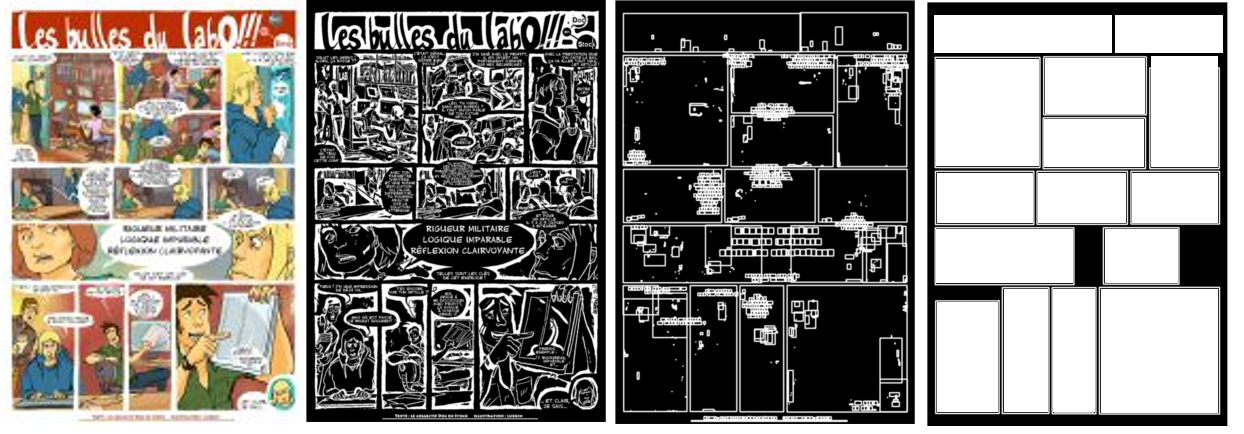
\includegraphics[width=1.0\textwidth]{panel_detection.png}
 %  \caption{Contour detection and filtering of panel.
 %  Original image, adaptive thresholding, contour bounding boxes and results mask of the outermost contours from left to right.}
 %  \label{fig:panel}
 % \end{figure}
%%%%%%%%%%%%%%%%%%%%%%%%%%%%%%%%%%%%%%%%%%%%%%%%%%%

%%%%%%%%%%%%%%%%%%%%%%%%%%%%%%%%%%%%%%%%%%%%%%%%%%%
\begin{figure}[!ht]	%trim=l b r t  width=0.5\textwidth, 
  \centering
	%\includegraphics[height=60mm]{figure/BUBBLEGOM_T01_P007_crop.jpg}
	%\includegraphics[trim= 0mm 0mm 0mm 0mm]{figure/BUBBLEGOM_T01_P007.jpg}
	\subfloat[Original image]{\label{fig:in:se:panel_img}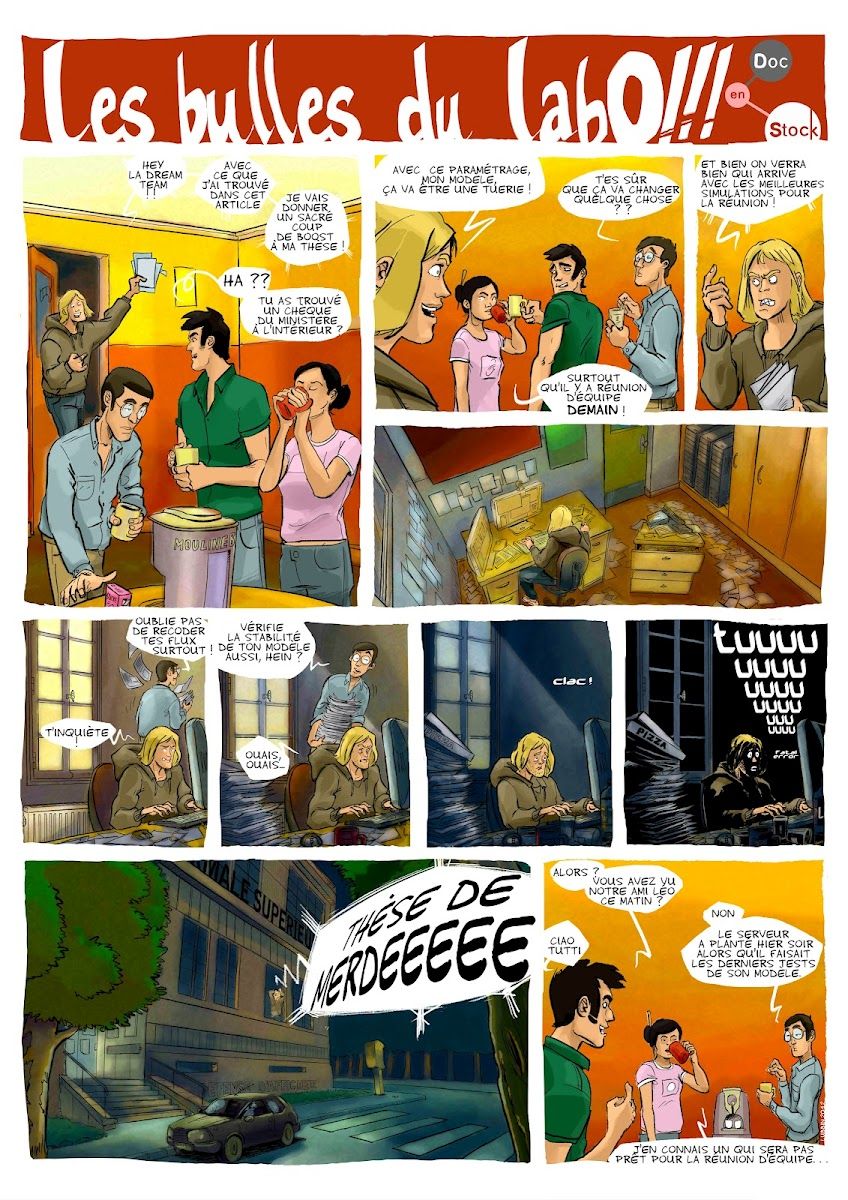
\includegraphics[trim= 0mm 0mm 0mm 0mm, clip, width=0.27\textwidth]{panel_img.jpg}}
	\hspace{1em}
	\subfloat[Binary segmentation]{\label{fig:se:panel_binary}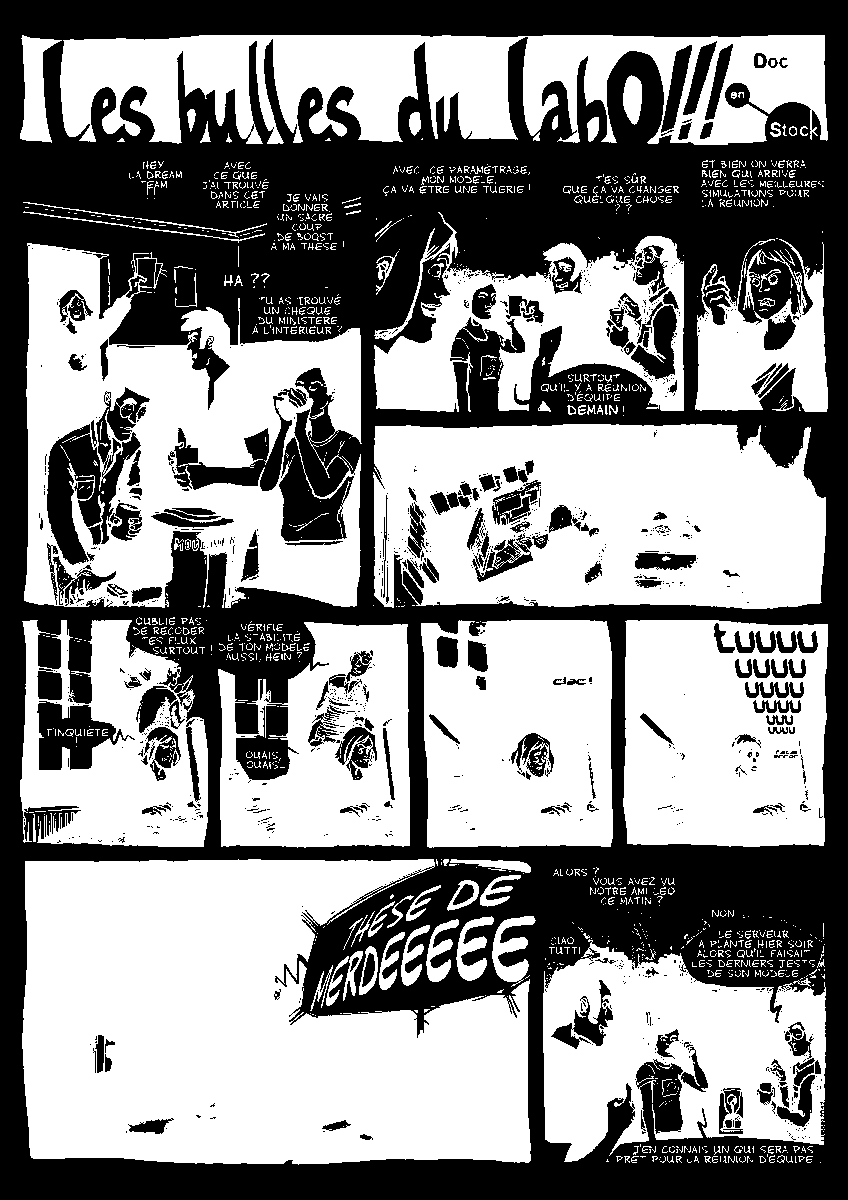
\includegraphics[trim= 0mm 0mm 0mm 0mm, clip, width=0.27\textwidth]{panel_binary.png}}
	\hspace{1em}
	\subfloat[Outermost contours]{\label{fig:in:panel_outermost_contours}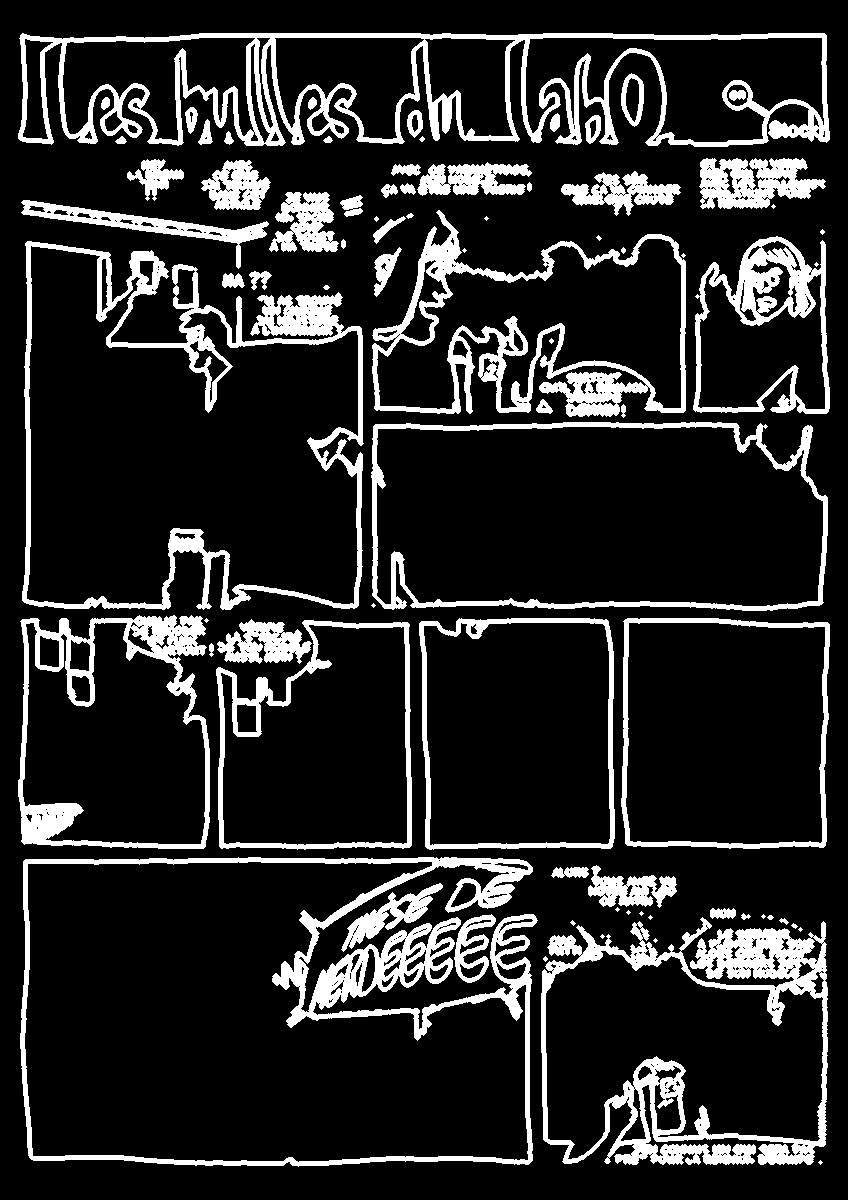
\includegraphics[trim= 0mm 0mm 0mm 0mm, clip, width=0.27\textwidth]{panel_all_contours.png}}
	\\
	\subfloat[Panel contours]{\label{fig:in:panel_big_contours}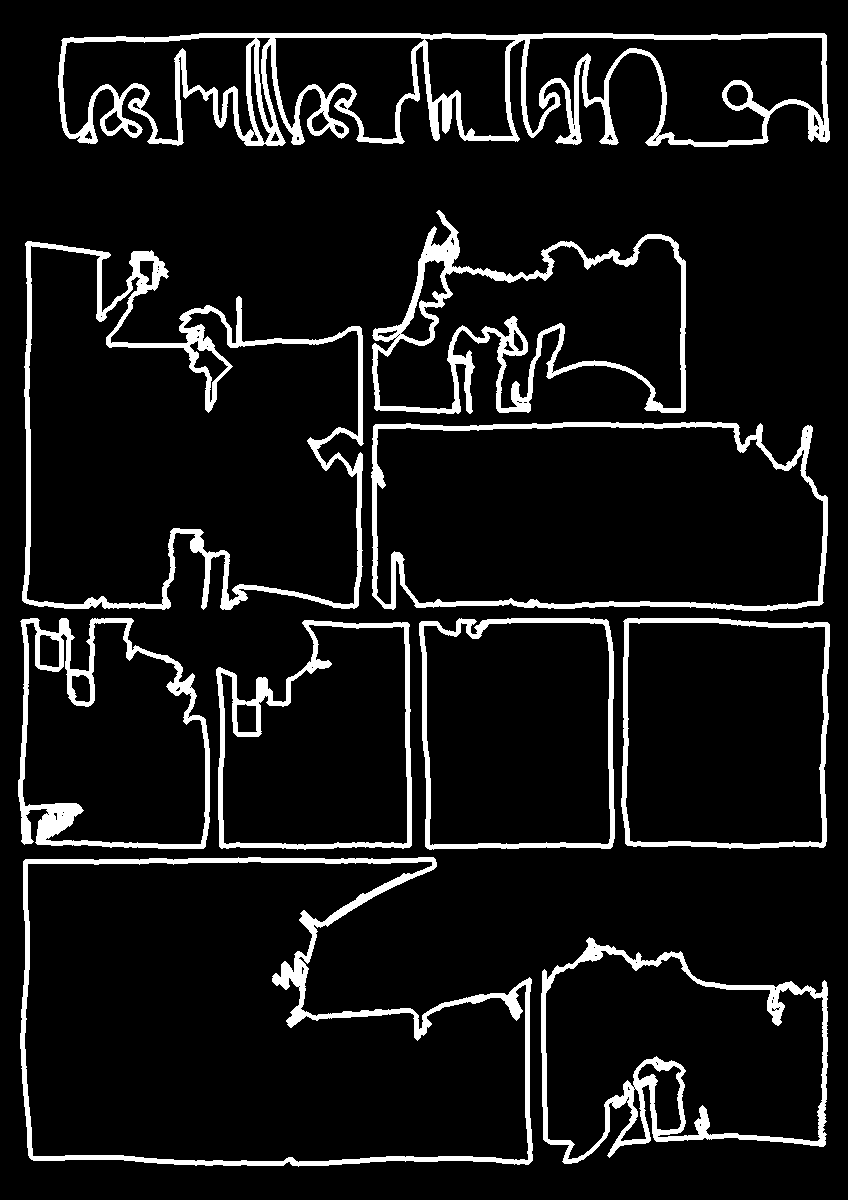
\includegraphics[trim= 0mm 0mm 0mm 0mm, clip, width=0.27\textwidth]{panel_big_contours.png}}	\hspace{1em}
	\subfloat[Panel contour hulls]{\label{fig:in:panel_big_contour_hull}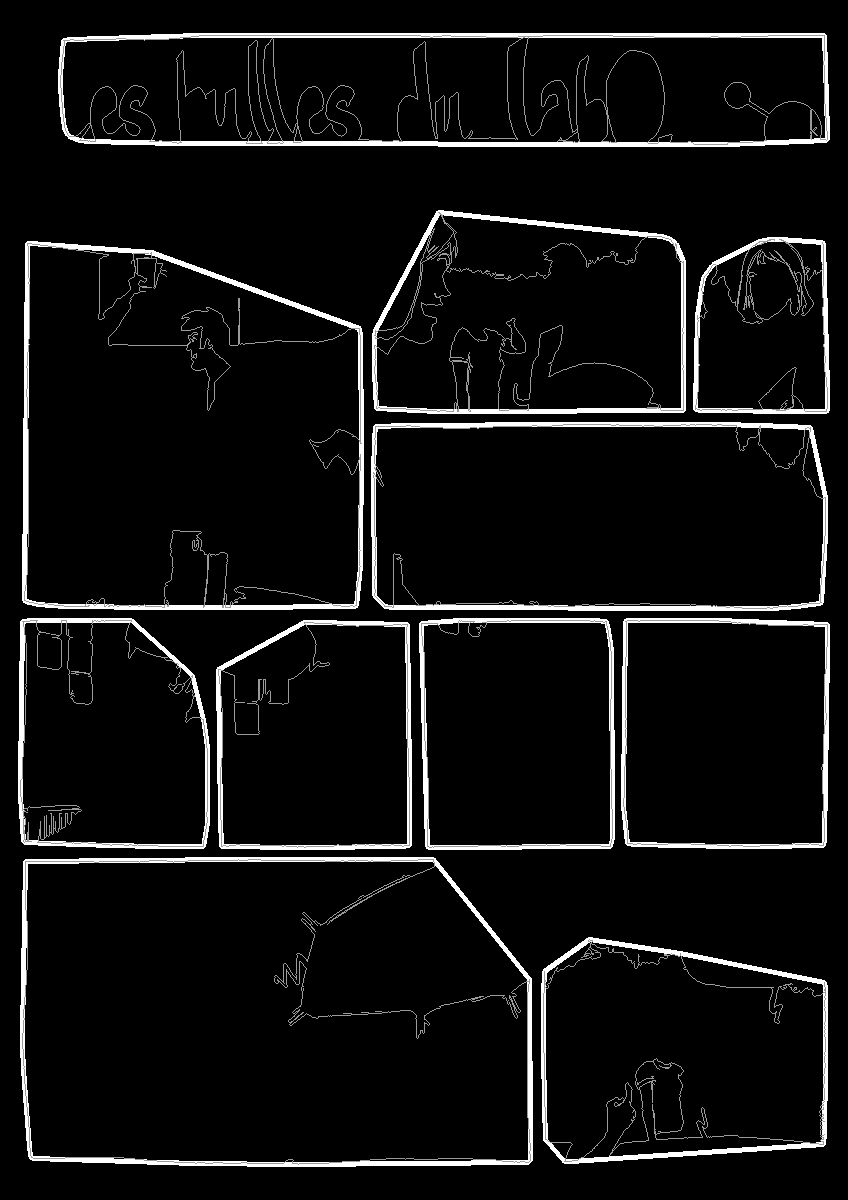
\includegraphics[trim= 0mm 0mm 0mm 0mm, clip, width=0.27\textwidth]{panel_big_contour_hull.png}}
	  \hspace{1em}
	\subfloat[Panel contour bounding boxes]{\label{fig:in:panels_detection_boxes}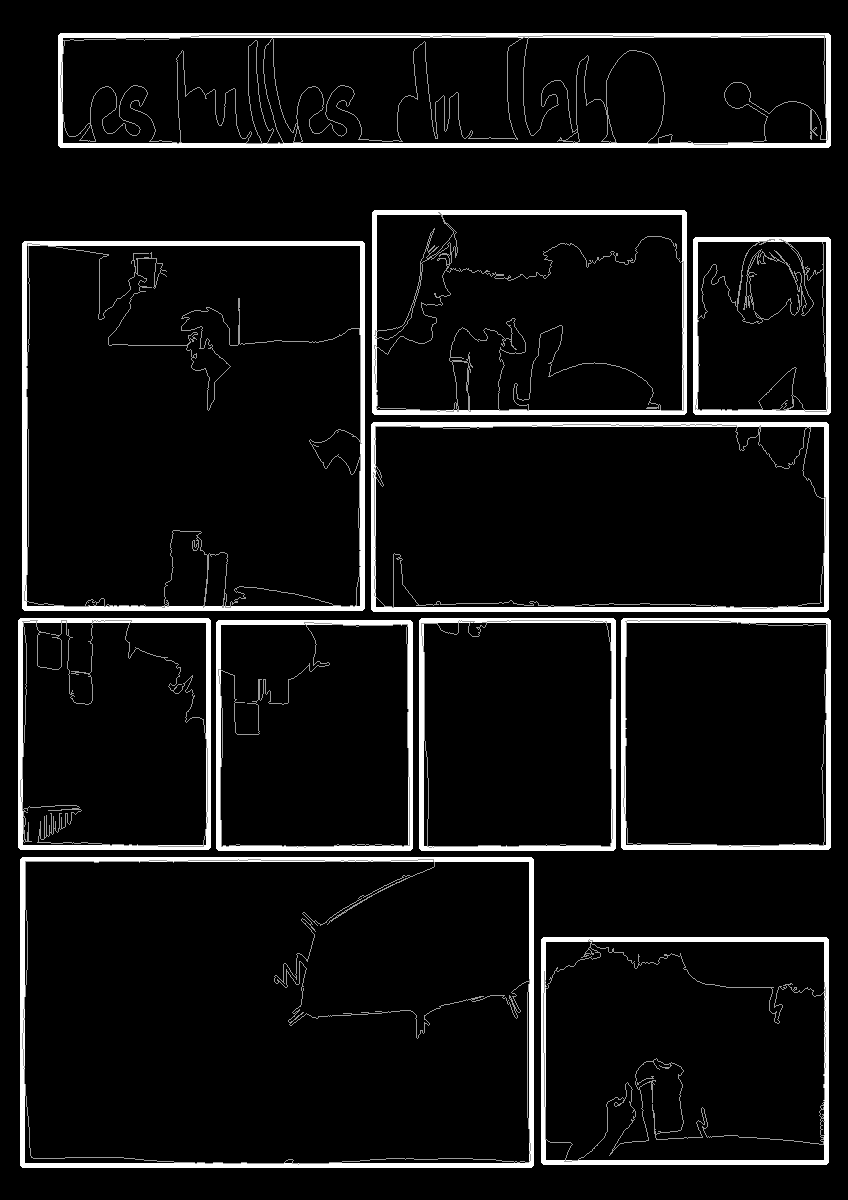
\includegraphics[trim= 0mm 0mm 0mm 0mm, clip, width=0.27\textwidth]{panels_detection_boxes.png}}
	  \caption[Independent panel extraction process]{Panel extraction process. Image credits:~\cite{Lubbin12}.}
	  \label{fig:in:panel_detection_process}
\end{figure}
%%%%%%%%%%%%%%%%%%%%%%%%%%%%%%%%%%%%%%%%%%%%%%%%%%%


\section{Text localisation and recognition} % (fold)
\label{sec:in:text_localisation_and_recognition}

In this section we present a method for automatic text localization in scanned comic books, an essential step towards an automatic comics understanding.
Our first intention is to localize multi-oriented text regions, independently from script and language, and separate them from the graphical content (text/graphic separation).
In document analysis systems, text recognition quality often relies on text localization.
This is particularly the case for comics which have a complex background.
We present how to take advantage of Optical Character Recognition systems (OCR) in order to improve text localisation.

\subsection{Introduction} % (fold)
\label{sub:in:text_introduction}

In comic book documents, text is mixed with graphical content which produces a lot false detections if we submit the whole image directly to an OCR system, usually coupled with a layer analysis pre-processing to avoid trying to recognize text in graphical region (e.g images, tables and formulas).
The mixture of typewritten, handwritten-like and handwritten text makes the task particularly difficult for comics.
Moreover, text presents a lot of variations (e.g. stroke, orientation, colour, size) that can cause many issues at both the localization and recognition levels.
Text localization aims to provide text-only (or graphics-free) images to a text recognition system in order to improve its accuracy and reduce computing time.
Knowing the positions of other elements in the image is a good clue for predicting text position because they are related to speech balloons (e.g. dialogue, thought), characters (e.g. graphic sound, illustration), panels (e.g. captions) or the page itself (e.g. page number, title, author name), this approach is discussed \ch{chap:knowledge}.

Few works concern text extraction in comics analysis literature (Section~\ref{sec:sota:text}) and most of them rely on speech balloon regions which make them dependent on other processing quality.
Here we want to avoid such dependency between processes.
From our knowledge, only Li~\cite{Li2013Unsupervised} proposed an independent and unsupervised speech text localization.
It is a two step analysis that first generates text lines using ``a set of very rigorous rules'' to test each pair of connected component and decide if they are candidate text regions or not.
From the first-round generated text lines, the method automatically learns a font set which is propagated to all text lines in the second-round and filters out non font-matched candidate regions.
The font set is generated from the distribution of heights and widths of the connected components that compose the candidate text line (composed by multi-segment characters).
The method is promising but there are nine rules in total that must be met to achieve text line extraction with several heuristics that are not discussed.
The experiments have been performed on 1000 images from 10 countries (balanced) but they are unfortunately not publicly available to assess their diversity and the genericity of this approach. 

The genericity is always a challenge for document image analysis, especially because this field of research is highly application dependent (Section~\ref{sec:document_image_analysis}).
Moreover, comic book images differ from classical documents in that they comprise complex backgrounds of a graphical nature.
They belong to the class of non-structured documents meaning there is no regular structure present for the prediction of text locations and no layout analysis method applicable if we consider all the diversity of comics.
Comics being unstructured graphical documents, combine the difficulties of both domains, making the task of text localization especially challenging.
To solve the particular problems which are provoked by the combination of complex background and unstructured documents, we propose a new text localization method.
% We improve the initial segmentation step to cope with complex backgrounds.
% Furthermore, we adapt the text line extraction method to cope with unstructured documents.

The contributions come at different levels. 
First, an adapted binary segmentation method is presented followed by a text/graphic separation algorithm based on the local contrast and neighbourhood similarities and finally, text recognition is used to verify the presence of textual information in the result.

% \subsection{Text localization} % (fold)
% \label{sub:te:text_localization}


\subsection{Bi-level segmentation}
\label{sec:in:segmentation}
Segmentation is a crucial step in many text localization methods.
Comic speech text is made of strokes, generally black on white, that we would like to isolate from the rest of the image content (background).
A perfect text segmentation would result to individual text letters represented by single connected components (Section~\ref{sec:ap:connected_component_labelling}).
The complex background of comic documents complicates this step.
Separating text from other elements in once is quite hard since we have no information about its position (independent approach) and it is similar to many other stroke in the image.
Therefore, we propose first to separate bright from dark regions and then classify text and non text regions using size and alignment properties only.
This approach is unsupervised and do not requires any training step.
Bright/dark region separation can be done using a bi-level segmentation algorithm.
Several approaches exist and their performance relies on the input data distribution.
If the input data are composed by only black or white pixels any method will do the work be it is rarely the case.
The best input would be a highly contrasted image where the feature of interest are concentrated in one of the extrema.
As we do not use the colour information, we convert the 3 channel colour image (RGB) into a single channel grey image.
There are several manners to create a grey-scale image from a colour image.
The first approach is to combine each pixel value from each colour channel with different weighting coefficients corresponding to the measured intensity perception of typical trichromat humans\footnote{\url{http://en.wikipedia.org/wiki/Grayscale}}, in order to produce a single value per pixel.
Another approach is to use only one channel but as the text we are interested in is not in red, green or blue (RGB colour space) it is irrelevant in our case.
Nevertheless, RGB colour space can easily be converted to a different colour space such as HSV or HSL that encodes colours as Hue, Saturation, Value or Luminance.
The luminance channel is particularly appropriate for bright and dark region separation~\cite{Ho2012}.

Even if looking at the pixel from the luminance point of view is more appropriate for our purpose, we still need to determine the threshold value that will best divide the grey value distribution into two clusters (Figure~\ref{fig:in:greyscale_text_pixel_distribution}).


% 	%%%%%%%%%%%%%%%%%%%%%%%%%%%%%%%%%%%%%%%%%%%%%%%%%%%
	\begin{figure}[h!]	%trim=l b r t  width=0.5\textwidth,
	  \centering
		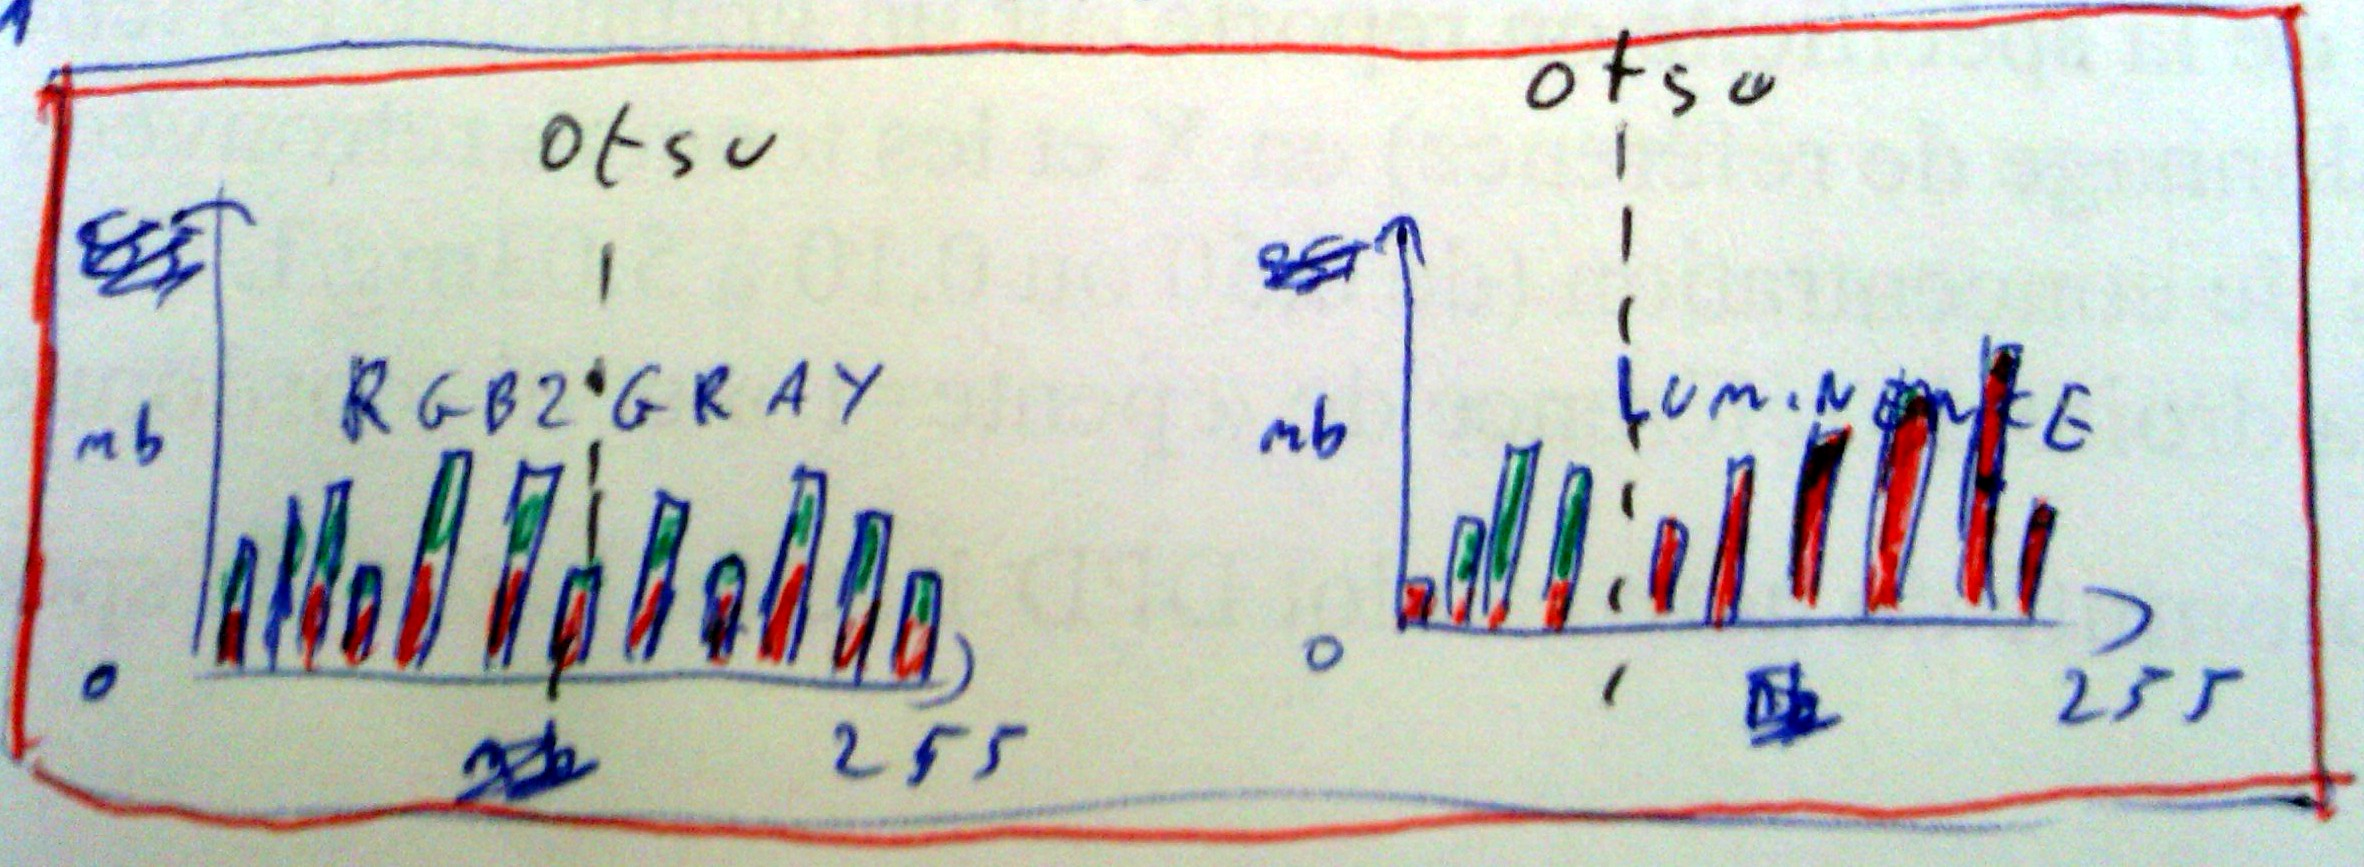
\includegraphics[trim= 0px 0px 0px 0px, clip, width=0.75\textwidth]{threshold_selection_methods.jpg}
		\caption[Grey scale image pixel value distribution for text and non text region]{Grey scale image pixel value distribution and text repartition. The percentage of pixel belonging to text regions are in green, others in red \modif{TODO: update figure}.}
		\label{fig:in:greyscale_text_pixel_distribution}
	\end{figure}
% 	%%%%%%%%%%%%%%%%%%%%%%%%%%%%%%%%%%%%%%%%%%%%%%%%%%%

Fixing a threshold value like Arai's method~\cite{Arai11} works only for few comics type with a same text background intensity (Figure~\ref{fig:in:threshold_selection_methods}).
This phenomenon is intrinsic to the nature of comics, as due to the design process they contain textured areas and loosely connected strokes that give rise to merged components at different thresholds.
This is intensified by the digitization and image compression process that adds further noise to the page (Section~\ref{sec:document_image_analysis}).
Instead of using a fixed threshold, we use the well known Otsu's threshold selection method that have been extensively use since decades for this purpose (Section~\ref{sub:ap:bi_threshold}).
Otsu's threshold is computed for each image and applied to the whole image assuming that the image have not been degraded locally.
In case of such local degradation (e.g. holes, crossed text, partial erasure, highlighting, tearing paper, stain), a local threshold selection method should be used (Section~\ref{sub:ap:bi_threshold}).


% 	%%%%%%%%%%%%%%%%%%%%%%%%%%%%%%%%%%%%%%%%%%%%%%%%%%%
	\begin{figure}[h!]	%trim=l b r t  width=0.5\textwidth,
	  \centering
		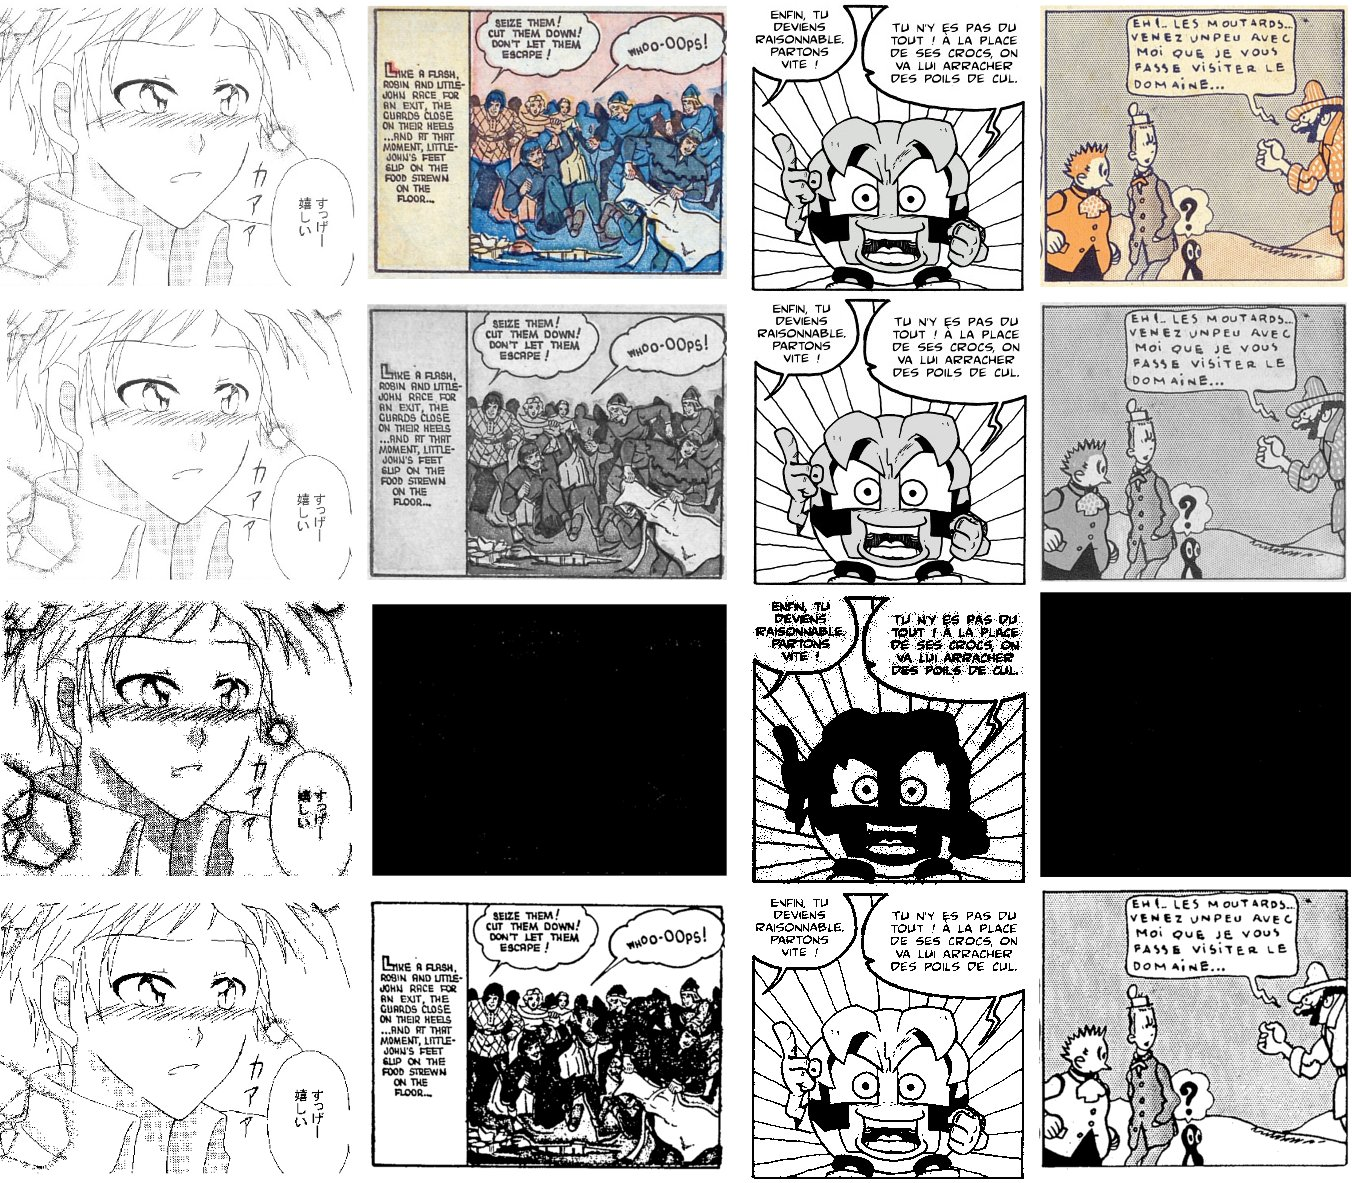
\includegraphics[trim= 0px 0px 0px 0px, clip, width=0.95\textwidth]{threshold_selection.jpg}
		\caption[Different threshold selection applied on a grey-scale image]{Different threshold selection methods applied on the luminance channel of several comics types. First row shows the original image of a selection of comic book parts. Second row shows the corresponding luminance channel of HSL colour space in a 8 bits grey-scale image. The third row represents the bi-level segmentation of the grey-scale image with a fixed threshold at 250 (as Arai~\cite{Arai11}) and fourth row shows the corresponding results using the automatic Otsu's threshold selection method.}
		\label{fig:in:threshold_selection_methods}
	\end{figure}
% 	%%%%%%%%%%%%%%%%%%%%%%%%%%%%%%%%%%%%%%%%%%%%%%%%%%%




%Typical thresholding methods would fail to segment the text because text is drawn with the same style of strokes as many other graphical elements in the page \modif{TODO: delete + explain the interest of choosing a good threshold, refer the standard Otsu from SOTA, its interest and the importance of its input (gray image). Assuming that text is written in dark over bright background or vice versa, we don't need the colour information (assuming we don't want to extract coloured text with this method). The widely used RGB2GRAY conversion combine the colour channel to produce a grey image. As we don't need the colour information, we convert RGB to HSL ans use the luminance layer as input for Otsu auto threshold selection. (illustrate the differences between Otsu'method applied on RGB2GRAY, H, S and L.)}.

%Therefore, we propose to improve the Otsu's threshold selection method~\ref{sub:ap:bi_threshold}.
%For a single page we assume that the text background brightness is similar around all the characters of the same page. However, in our case, the optimal segmentation threshold differs for every single page of comics depending on the background colour of the text areas. The method is based on the observation that choosing the threshold too low, as well as choosing the threshold too high leads to an over segmentation of the connected components (CC) (Figure~\ref{fig:in:bin}).

	%%%%%%%%%%%%%%%%%%%%%%%%%%%%%%%%%%%%%%%%%%%%%%%%%%%
	% \begin{figure}[h!] %trim=l b r t
	%   \begin{center}$
	%     \begin{array}{cccc}
	%       \fbox{\includegraphics[trim= 597px 20px 500px 400px, clip, width=0.22\textwidth]{bin_50.png}} &
	%       \fbox{\includegraphics[trim= 597px 20px 500px 400px, clip, width=0.22\textwidth]{bin_80.png}}  \\
	%       \fbox{\includegraphics[trim= 597px 20px 500px 400px, clip, width=0.22\textwidth]{bin_120.png}} &
	%       \fbox{\includegraphics[trim= 597px 20px 500px 400px, clip, width=0.22\textwidth]{bin_200.png}}
	%     \end{array}$
	%   \end{center}
	% \caption[Threshold selection effect]{Segmentation at different threshold levels from the lower top-left to the higher bottom-right (threshold = 50, 100, 150, 200). We observe that the number of CC increases when the dark lines are cut and also when background start to appear as salt and paper noise. Image credits:~\cite{Roudier11}.}
	% \label{fig:in:bin}
	% \end{figure}
	%%%%%%%%%%%%%%%%%%%%%%%%%%%%%%%%%%%%%%%%%%%%%%%%%%%


%Our method, Minimum Connected Components Thresholding (MCCT), automatically finds the right threshold by computing the number of CC for different threshold levels in a range of values from $th_{min}$ to $th_{max}$ and selecting the one that produces the minimum number of CC between the  (in a 8 bits grey image). %We defined a range from 100 to 230 (grayscale value of 8 bits image) for the binarization threshold.
% Our method, Minimum Connected Components Thresholding (MCCT), improves Otsu's threshold selection method by shifting the threshold according to the number of CC that are created.
% Given an Otsu's threshold $th_i$, we segment the image at different threshold centred on $th_i$ (e.g. $th_{i-1}$ to $th_{i-n}$ and $th_{i+1}$ to $th_{i+n}$) and select the one that produces the minimum number of CC (Figure~\ref{fig:in:CC_graph}).
% Note that the threshold selection method requires a single channel image (e.g intensity, luminance) %We defined a range from 100 to 230 (grayscale value of 8 bits image) for the binarization threshold.
% \modif{TODO: experiment and remove $th_{min}$ and $th_{max}$ if possible.}

% Then we find the first minimal number of CC. See example on figure~\ref{fig:in:CC_graph}.
% Note, that the optimal threshold is correctly predicted by MCCT as it corresponds to the bottom-left image figure~\ref{fig:in:bin}.

% 
% 	%%%%%%%%%%%%%%%%%%%%%%%%%%%%%%%%%%%%%%%%%%%%%%%%%%%
	% \begin{figure}[h!]	%trim=l b r t  width=0.5\textwidth,
	%   \centering
	% 	\includegraphics[trim= 0px 0px 0px 0px, clip, width=0.75\textwidth]{CC_graph_source_one_curve.pdf}
	% 	\caption[Evolution of the number of connected-component]{Example of number of CC function of the segmentation threshold. In this case, $th_{min}=100$, $th_{max}=230$ and our algorithm found 150 as optimal threshold threshold \modif{TODO: update with more credible figure from 0 to 255 (average CC evolution instead of single image???)}.}
	% 	\label{fig:in:CC_graph}
	% \end{figure}
% 	%%%%%%%%%%%%%%%%%%%%%%%%%%%%%%%%%%%%%%%%%%%%%%%%%%%

As an alternative segmentation method, we also tried to extract text region using the Maximally Stable Extremal Region (MSER) algorithm~\cite{matas2004robust}.
This algorithm was better than the proposed method only for text region of type onomatopoeia but produced an excess of false detections as in general a lot of the graphical elements are equally stable as the text (flat regions).

% We also try the well known Otsu~\cite{otsu79} algorithm \modif{TODO; justify or delete}.
%\footnote{http://www.labbookpages.co.uk/software/imgProc/otsuThreshold.html}
% (see section~\ref{sec:experiments}).

%Our method is similar to Maximally Stable Extremal Region (MSER) algorithm~\cite{Matas02} because we also try to find an extrema. However, MSER accuracy is low because of the stroke of the text which is very thin compare to the other elements present in the page. This algorithm require a minimum number of stable regions as threshold which as to be very low in our case (text is small region) and a lot of other regions will remain then.

\subsection{Text/graphics separation}
\label{sec:in:textgraphicseparation}
%For the extraction we use CC algorithm for the reason presented in~\ref{sec:segmentation}. We considered only the CC that are black on a white background in the binary image (see figure~\ref{fig:in:bw_wb}). %For the white CC on black background see experiments (section~\ref{sec:experiments}).

After the binary segmentation step we apply the connected-component (CC) labelling method (Section~\ref{sec:ap:connected_component_labelling}) to extract the black strokes as many previous work in the literature (Section~\ref{sec:sota:text}).
At this stage, the extracted components may correspond to part of drawing, single letters or a sequence of letters if some are connected (Figure~\ref{fig:in:detach_attach_letter}).
The objective of this section is to separate the last two categories from the first one.
Note that connected letters will not affect our results (if they are part of the same word) because the expected output is at text line level.


	%%%%%%%%%%%%%%%%%%%%%%%%%%%%%%%%%%%%%%%%%%%%%%%%%%%
	\begin{figure}[h!]%trim=l b r t
	  \begin{center}$
	    \begin{array}{cc}
	     \includegraphics[height=7mm]{deattached_letter.png} &
	      \includegraphics[height=7mm]{attached_letter.png}
	    \end{array}$
	  \end{center}
	\caption[Inter-connected letters]{Example of connection between connected components. On the left, a word with six well separated letters, on the right a word detected as two pairs of attached letters because of the handwriting variability and segmentation process.}
	\label{fig:in:detach_attach_letter}
	\end{figure}
	%%%%%%%%%%%%%%%%%%%%%%%%%%%%%%%%%%%%%%%%%%%%%%%%%%%


%The main drawback is when letters are in contact with different lines or drawing elements (see figure~\ref{fig:contact_letter}). We did not work on this assuming that it not so common in comics.

	%%%%%%%%%%%%%%%%%%%%%%%%%%%%%%%%%%%%%%%%%%%%%%%%%%%
% 	\begin{figure}
% 	  \begin{center}$
% 	    \begin{array}{cc}
% 	      \includegraphics[height=15mm]{fig/BW_CC.png} &
% 	      \includegraphics[height=15mm]{fig/WB_CC.png}
% 	    \end{array}$
% 	  \end{center}
% 	\caption{CC black on white (left) and white on black (right) from the same page.}
% \label{fig:in:bw_wb}
% 	\end{figure}
	%%%%%%%%%%%%%%%%%%%%%%%%%%%%%%%%%%%%%%%%%%%%%%%%%%%

%\subsubsection{Letter filtering}

We propose a number of rules, applied sequentially, to separate graphics from text. Due to the wide variety of text usage in comic albums, the method should be size, translation, rotation, scale and contrast invariant. In addition, it should be robust to text-less pages which may appear randomly within an album. From all the components extracted by the CC algorithm, we use three filtering rules to select only the ones corresponding to potential textual elements.

%The idea is to keep only the groups of very contrasted CC.

	%%%%%%%%%%%%%%%%%%%%%%%%%%%%%%%%%%%%%%%%%%%%%%%%%%%
% 	\begin{figure}[!ht]	%trim=l b r t  width=0.5\textwidth,
% 	  \centering
% 		\includegraphics[height=27mm]{fig/contact_letter.png}
% 		\caption{Example of letter in contact with other elements. In this case the bounding box are in blue  (rectangle), in this case of the component 'J' is the whole balloon.}
% 		\label{fig:contact_letter}
% 	\end{figure}
	%%%%%%%%%%%%%%%%%%%%%%%%%%%%%%%%%%%%%%%%%%%%%%%%%%%

% \begin{itemize}

Rule 1: we compare the standard deviation of the grey-levels of the luminance layer of each CC bounding boxes (Figure~\ref{fig:in:std_dev}) with the contrast ratio of the page to make a high/low local contrast CC separation, similarly to~\cite{Li2013Unsupervised} using the Mahalanobis distance~\cite{mahalanobis1936generalized,de2000mahalanobis}.
We assume a Gaussian distribution of the grey level pixels but other distribution are under study. The contrast ratio of the page is the absolute difference between the minimum and the maximum grey-levels found on the page.
% In order to avoid artefacts pixel values, we apply a median filtering as preprocessing.
%The higher the standard deviation is, the higher the probably of being a letter.

%The minimum of difference between letter standard deviation ($\sigma$) and the page content ratio was 1/2 (according to $\sigma=68.27\%$ of the values)

	%%%%%%%%%%%%%%%%%%%%%%%%%%%%%%%%%%%%%%%%%%%%%%%%%%%
	\begin{figure}[h!]
	  \begin{center}$
	    \begin{array}{cc}
	      \includegraphics[height=10mm]{letter_N_gs.png} &
	      \includegraphics[height=10mm]{letter_eyeblow_gs.png}
	    \end{array}$
	  \end{center}
	  \caption[Mean and standard variation values of connected-component bounding boxes]{Example of mean ($\mu$) and standard deviation ($\sigma$) values of two CC bounding box regions. For the letter ``N'',  $\mu,\sigma=[167,84]$ and for the eyebrow $\mu,\sigma=[110,57]$. %In this case the contrast ratio of the page was 255, N is high contrasted 2$\sigma > 255 * 50\% $ unlike the eyebrow.
	  }
	  \label{fig:in:std_dev}
	\end{figure}
	%%%%%%%%%%%%%%%%%%%%%%%%%%%%%%%%%%%%%%%%%%%%%%%%%%%

% Rule 2: we apply a topological filtering that consists in removing all the CC that overlap with others assuming that the CC of a letter can not contain another CC, similar to~\cite{Kasar07}.
% In our study we consider only the black on white CC (Figure~\ref{fig:in:bw_wb}).

% 	%%%%%%%%%%%%%%%%%%%%%%%%%%%%%%%%%%%%%%%%%%%%%%%%%%%
% 	\begin{figure}[h!]%trim=l b r t
% 	  \begin{center}$
% 	    \begin{array}{cc}
% 	      \includegraphics[height=8mm, trim= 0px 4px 0px 3px, clip]{BW_bin_CC.png} &
% 	      \includegraphics[height=8mm, trim= 0px 4px 0px 3px, clip]{WB_bin_CC.png}
% 	    \end{array}$
% 	  \end{center}
% 	\caption[Difference between black over white and white over black connected-components]{On the left, an example of black over white CC bounding box (red rectangle) and on the right side, a white over black (the white inside region of the letter ``A'').}
% 	\label{fig:in:bw_wb}
% 	\end{figure}
% 	%%%%%%%%%%%%%%%%%%%%%%%%%%%%%%%%%%%%%%%%%%%%%%%%%%%


Rule 2: we verify that each letter $l_i$ is surrounded by other letters $l_j$ (with $_j\in{[0,n]}$) which is intrinsic to the design of text (grouping characters in words and text lines).
To do so, we check for similar in height components in a local region equal to the size of the component's bounding box extended to its left/right/top/bottom directions (Figure~\ref{fig:in:4_direction}). For instance, $l_i$ is considered similar in height to $l_i$ if $abs(l_i.height - l_j.height)<a*l_i.height$ ($a=$similarity offset). %If yes then both are considered as letter.
%\end{enumerate}


	%%%%%%%%%%%%%%%%%%%%%%%%%%%%%%%%%%%%%%%%%%%%%%%%%%%
	\begin{figure}[h!]	%trim=l b r t  width=0.5\textwidth,
	  \centering
		\includegraphics[width=0.50\textwidth]{4_direction.png}
		\caption[Text candidate region neighbourhood analysis]{Neighbourhood analysis for text and non text classification (rule 3). The area of the bounding box of the letter ``A'' is extended in four directions around the letter ``A'' to check if any other letter (blue rectangles) overlaps with it. In this example, there are two overlapping components (red dashed rectangles) at the right and the bottom of the letter ``A''. The component is thus accepted as a text letter candidate.}
		\label{fig:in:4_direction}
	\end{figure}
	%%%%%%%%%%%%%%%%%%%%%%%%%%%%%%%%%%%%%%%%%%%%%%%%%%%

Rule 3:
we check all the CC bounding boxes pairs that overlap more than $b$\% each other.
We remove the biggest from each pairs.

\subsection{Text line generation} % (fold)
\label{sub:in:text_line_generation}
As already mentioned Section~\ref{par:se:letter_to_line}, the gap between text component (e.g. letter or attached letters, word) and text lines can vary significantly.
Here we use the same method as presented in Section~\ref{par:se:letter_to_line} to group text component into text lines considering only the text height (or width for vertical text).
%We can group text parts to text lines using the method presented Section~\ref{par:se:letter_to_line}.

% subsection text_line_generation (end)
% \end{itemize}


\subsection{Text recognition} % (fold)
\label{sub:in:text_recognition}
Automatic text recognition has been studied for many years, today OCR systems are very efficient for standard fonts but not optimized for comics fonts which are mostly handwritten.
The principal interest of text recognition is the ability of searching images by using keywords which opens up many applications (Section~\ref{sec:sota:text}).
Text recognition applied to comics is really challenging because it includes most of the difficulties from text recognition in document analysis domain if we consider all the type of text that composed the comics.
From typewritten to handwritten and free-form text in uniform to complex background including image noise, text deformation and overlapping (Figure~\ref{fig:in:texlines_example}).
Note that the text is mainly written in upper case for Latin scripts in comics which reduce the complexity of recognition.

%%%%%%%%%%%%%%%%%%%%%%%%%%%%%%%%%%%%%%%%%%%%%%%%%%%
 \begin{figure}[!ht]  %trim=l b r t  width=0.5\textwidth,
   \centering
  \fbox{\includegraphics[trim= 1px 1px 3px 2px, clip, width=0.75\textwidth]{text_line_examples.png}}
  \caption[Examples of text lines from comics images]{Examples of text lines from comics images.}
  \label{fig:in:texlines_example}
 \end{figure}
%%%%%%%%%%%%%%%%%%%%%%%%%%%%%%%%%%%%%%%%%%%%%%%%%%%

% Text recognition in comics would allow full-text search, tagging, image description, comic character labelling etc.
Text recognition for comics requires an extensive work to be addressed properly, which is out of the scope of this thesis work.
Even if standard OCR recognition rate is not yet acceptable yet for full-text based application in comics, they can help at separating text/non text regions.

We pass each text line candidate through an OCR system to validate its content.
The validation criterion is that the OCR recognize at least one alphabetical symbol within the candidate region, else it is rejected.
The text line are composed by 12 character in average which give a good chances to OCR to recognize at least one of them (Section~\ref{sec:dataset_description}).


% Nevertheless, we measure the performance of current OCR systems Section~\ref{sub:ex:text_extraction_recognition_evaluation}.

% section text_localisation_and_recognition (end)

\section{Balloon extraction and classification}
\label{sec:in:balloon}

In this section we present a method for pixel level balloon extraction and for balloon classification.
Balloon extraction does not requires previous text extraction unlike the method presented Section~\ref{sub:se:regular_balloon_extraction} but uses a careful analysis of the region content (e.g. similarities, spacial organisation) to predict which are most likely balloon regions.
Balloon contour and shape information differences are presented and a contour-based classification method is detailed for ``smooth'', ``wavy'' and ``zigzag'' classes that may correspond to ``dialogue'', ``thought'' and ``exclamation'' in a higher level context (\ch{chap:knowledge}).

\subsection{Balloon segmentation} % (fold)
\label{sub:in:balloon_segmentation}
From the reviewed methods Section~\ref{sec:sota:balloon_segmentation}, we can see that the text position often help in the localization and then segmentation of speech balloons.
The issue in relying on text extraction is that we become dependent of its performance.
The text extraction in comics images is still a challenging problem (Section~\ref{sec:in:text_localisation_and_recognition}), it is a very hard assumption to assume the text extraction will work perfectly. 
% two of them~\cite{Ho2012,rigaud2013active} are based on text position which relies on the text extractor performance.
Instead of relaying on the text detection we propose to keep both processes independent in order to avoid errors of propagation.
% independent the low level processing.
In a similar way, Arai's method~\cite{Arai11} does not use text position but connected component filtering based on heuristics (fixed thresholds for binary image segmentation, blob size, number of white pixels, number of contained straight lines and width to length ratio). 
We propose a more adaptive method in order to handle various comics styles (e.g. colour, B\&W), image formats (e.g. A4, A5, portrait, landscape) and digitization variations (e.g. scanning device, camera capture).

The use of fixed thresholds for the segmentation process such as~\cite{Arai11} is a strong assumption about the image background nature.
It only works for comics from the same style and digitized under the same light condition.
We propose to relax the constraint by using Otsu's threshold selection method~\cite{otsu79} to make a global binary segmentation of the grey-scale image.
The binary segmentation creates a lot of small connected components on textured images, we prune it by removing the connected components that are classified as ``noise'' by the algorithm presented Section~\ref{sec:se:panel_and_text}.
%~\cite{Rigaud2012LNCS} (class with the minimum average height).
% and then we add one time the standard deviation value to avoid opening black contour by choosing a low threshold such as~\cite{.
We extract connected components from the binary image and analyse their parent-child relationship to make a first selection of candidate components and then analyse the spatial organisation of the set of children $CH=\{ch_1, ch_2,...,ch_n\}$ to compute a confidence value for each parent $P=\{p_1, p_2,...,p_m\}$ that serve as final filtering criterion (Figure~\ref{fig:in:balloon_binarisation}).

%%%%%%%%%%%%%%%%%%%%%%%%%%%%%%%%%%%%%%%%%%%%%%%%%%%
 \begin{figure}[!ht]  %trim=l b r t  width=0.5\textwidth,
   \centering
  \includegraphics[width=0.9\textwidth]{closed_balloon_process.png}
  \caption[Balloon extraction process]{Balloon extraction process. Original image, binary segmentation, contour detection (connected components) and result mask from left to right.}
  \label{fig:in:balloon_binarisation}
 \end{figure}
%%%%%%%%%%%%%%%%%%%%%%%%%%%%%%%%%%%%%%%%%%%%%%%%%%%

We assume that a balloon has a minimum of children $minNbChildren$ which are horizontally or vertically aligned and centred inside the balloon region (property of text).
The percentage of alignment $align$ is computed for each child $ch_i$ considering $CHA(ch_i)$ the subset of children that are aligned to $ch_i$ (Equation~\ref{eq:in:balloon_alignment}).

\begin{equation}
	\label{eq:in:balloon_alignment}
	align(ch_i) = \frac{|CHA(ch_i)|}{n}
\end{equation}
where $|CHA(ch_i)|$ is the number of aligned children and $n$ the total number of children.

%TODO: Dimos on 2014-06-30: use a min criteria isAligned IF more than N=4 chidlen are aligned with the current one + decide the percentage of children that are valid over all the children of the parent -> confidence value.

For instance, if we consider two children $E$ and $F$, they are considered as aligned (vertically) if the following conditions are verified $centroidF_x \in [minE_x, maxE_x]$ and $centroidE_x \in [minF_x, maxF_x]$ where $min_x$ and $max_x$ are the left and right limits on the horizontal axis.
The child $F$ is also considered to be aligned (horizontally) to $E$ by changing $x$ to $y$ which become the top and bottom bounding box limits.

We use the difference of alignment between the balloon candidate and its children as a clue about its probability of being a real balloon in image.
This is similar to the text dependent balloon extraction method presented Section~\ref{sec:se:panel_and_text}.
The difference is that here we have no idea about the nature of the children (not detected as text before).
This independent balloon extraction method can be seen as an ``intelligent'' balloon extractor that embeds a part of a the domain knowledge related to text (balloons are expected to contain text).
The difference of alignment is computed for the horizontal ($d_x$) and the vertical ($d_y$) axis from the Euclidean distance between the parent and children hull centroids (Figure~\ref{fig:in:coaxial_alignment}).


    %%%%%%%%%%%%%%%%%%%%%%%%%%%%%%%%%%%%%%%%%%%%%%%%%%%%%%%%
    \begin{figure}[ht]%trim=l b r t  width=0.5\textwidth,  
      \centering
      \includegraphics[trim= 0px 15px 80px 24px, clip, width=0.35\textwidth]{coaxial_alignment.png}
    \caption[Balloon content alignment measures]{Horizontal and vertical alignment measurement between the centroids of the balloon (dark cross) and the children hull (clear cross). The children hull is the grey region included in the balloon.}
    \label{fig:in:coaxial_alignment}
    \end{figure}
    %%%%%%%%%%%%%%%%%%%%%%%%%%%%%%%%%%%%%%%%%%%%%%%%%%%%%%%%

Both differences $d_x$ and $d_y$ are normalized between zero and one as a percentage of the balloon (parent) width and height respectively.
The average of the alignments, $\overline{align}$, $d_x$ and $d_y$ gives a confidence value for each candidate of $P$ (Formula~\ref{eq:in:balloon_confidence_value}).

\begin{equation}
	\label{eq:in:balloon_confidence_value}
	C_{balloon} = \frac{1}{3} * \Big( \overline{align} + d_x + d_y \Big)
\end{equation}

The confidence value is used for balloon and non balloon decision (Section~\ref{sub:ex:balloon_extraction_evaluation}).
%TODO: justify the product with fuzzy logic approaches for information combination

% This work have been submitted to the International Journal on Document Analysis and Recognition~\ref{???}.

Tail detection is not treated as an independent extraction because it is part of balloons and never appears without being related to a regular or implicit balloon.
Please refer to Section~\ref{sec:se:from_balloon_to_tail} for more detail about tail detection.

\subsection{Balloon classification} % (fold)
\label{sub:in:balloon_classification}

Speech balloon classification is a real challenge if we consider a lot of different comics styles.
First, each author has his own representation of the speech sounds. Second, the reader interpretation is subjective (each balloon style is interpreted in comparison to the already read balloon styles).
For those reasons, it is really hard to directly define the purpose (e.g. dialogue, thought and exclamation) of a speech balloon without knowing its context in the story.
In fact, the context is defined by both graphic (e.g. other strokes, protagonists personality) and textual (e.g. vocabulary, punctuation) elements.
For instance, Figure~\ref{fig:in:contour_style} shows six different speech balloon comics styles where we can note the difficulty to assign one class for each balloon without knowing others balloon shapes and reading the contained text.

% Note, speech balloon classification is complementary to speech balloon extraction that has already been studied using white connected component extraction and filtering~\cite{Arai11,Ho2012} or active contour model~\cite{Rigaud2013ICDAR}.


	%%%%%%%%%%%%%%%%%%%%%%%%%%%%%%%%%%%%%%%%%%%%%%%%%%
	\begin{figure}[!ht]	%trim=l b r t  width=0.5\textwidth,
	  \centering
		\fbox{\includegraphics[trim = 0mm 1mm 0mm 0mm, clip, width=0.8\textwidth]{contour_style.png}}
		\caption[Relation between speech balloon shape and contour informations]{Examples of speech balloons from 6 comics albums (rows) that represent 3 different expressions (columns).}
		\label{fig:in:contour_style}
	\end{figure}
	%%%%%%%%%%%%%%%%%%%%%%%%%%%%%%%%%%%%%%%%%%%%%%%%%%


% Balloon classification aims to automatically determine which balloons are for normal speech, though and exclamation.
% This information add a new level of understanding of the comics image content.
% From our knowledge, speech balloon classification has not been studied before.
% It is related to contour classification in planar images.



% \subsubsection{Proposed method}
% \label{sec:in:contour_classification}

The input of the proposed method is a pixel-level balloon contour detection, such as proposed in Sections~\ref{sub:se:regular_balloon_extraction} and~\ref{sec:in:balloon}.

The shape and the contour of a balloon contain different type of information.
The shape (e.g. rectangle, square, circle, oval) does not provide a lot of information about how the text is spoken, it is more related to the style of the comics and the structure of the panel.
However, the contour contains the speech tone information according to the different patterns which are along the boundary of the balloon.

% In this section we detail how we perform the shape and contour separation, the contour description and finally the classification using a Bayesian classifier.

% The next section details the balloon shape/contour information separation, description and classification.
% Section~\ref{sec:experiments} evaluates the proposed method by showing the results of speech balloon classification.
% Finally, section~\ref{sec:discussion} and~\ref{sec:conclusion} discuss and conclude this work.


\subsubsection{Shape/contour separation}
\label{sec:contour_detection}
As introduced in Section~\ref{sec:sota:balloon_segmentation}, the discriminant information for speech balloon classification is not provided by the global shape but by the contour variations. 

First, we propose to represent the speech balloon as a time series (one dimensional signal over $360^\circ$) which corresponds to the distance in number of pixels between the balloon barycentre and the contour points. 

Second, we perform a shape/contour separation to be able to analyse only the contour variation (including the balloon tail). We approximate the global shape $s$ by smoothing the original signal $o$ using a sliding window of size $M$ and subtracting the result from the original signal to preserve only the contour information $c$ independently from the shape: $c = o - s$. The smoothed contour $s$ is a centred local average of $o$ (Formula~\ref{eq:be:smooth}).
Examples are given Figure~\ref{fig:be:time_series}.

% and normalized by the letter height $\bar{H}$ (see eq.~\ref{eq:avg_height}).

	%%%%%%%%%%%%%%%%%%%%%%%%%%%%%%%%%%%%%%%%%%%%%%%%%%
	\begin{figure}[!ht]	%trim=l b r t  width=0.5\textwidth,
	  \centering
		\fbox{\includegraphics[ width=0.9\textwidth]{time_series.png}}
		\caption[Balloon contour time series]{Balloon detection, time series representation and shape/contour separation. Left column represents balloon detection with the barycentre (white hole) and the starting point (top left half square). Middle column represents the distance between the barycentre and the balloon boundary over $360^\circ$ (clockwise) where the original signal $o$ is in blue and the smoothed signal $s$ in red. Right column is the difference between $s$ and $o$.}
		\label{fig:be:time_series}
	\end{figure}
	%%%%%%%%%%%%%%%%%%%%%%%%%%%%%%%%%%%%%%%%%%%%%%%%%%

\begin{equation}
\label{eq:be:smooth}
 s(o) = \frac{1}{M} * \sum_{-M/2}^{+M/2} o
\end{equation}
% where $M$ is the window size.% For instance, if $M=10$ and $i=20 \in[0, 360]$, $s_{20}$ will be the average of the distances between $o_{15}$ to $o_{25}$.



\subsubsection{Contour description}
\label{sec:be:description}
%In this section we propose a method to classify speech balloon contours by using time series representation. %An alternative could be based on the center of mass~\cite{Keogh2006}.

Contour description encodes the contour variations relatively to the balloons size to be invariant to page format and definition.

The level of variation can be computed from different features, the main difficulty is to be invariant to the comics drawing diversity. 
In this study, we describe the contour signal $c$ by using a variance-based two dimensional descriptor, more precisely the standard deviation $\sigma$. The variance or the standard deviation have the advantage to be simple and generic at describing any data distribution by measuring the data dispersion which is what we need if we aim at measuring the difference of dispersion between the original and the smoothed contours. In order to be invariant to the image definition and scale, we normalize each feature of the descriptor by the original signal average $\bar{o}$ (average radius).
%The first dimension is the global contour signal variance and the second is the difference between the top and bottom part variances. 

The first dimension aims to differentiates contours which have high variations (``zigzag'' type) from the others (``wavy'' and ``smooth'' types). The second dimension aims to discriminate ``wavy'' and ``smooth'' types according to the standard deviation of the superior and inferior signal part from the average $\bar{c}$. For instance, if a contour has a higher standard deviation in the below signal part than the above signal part (according to the average $\bar{c}$) then the contour has more peaks in the direction of its barycentre than the opposite, which is not a characteristic of the ``smooth'' type but ``wavy''.

The first feature $f_1$ consists in measuring the standard deviation $\sigma_c$ of the contour signal $c$ normalized by the original signal average $\bar{o}$ (Formula~\ref{eq:be:distortion}).


\begin{equation}\label{eq:be:distortion}
 f_1 = \frac{\sigma_c}{\bar{o}}% * \sum_{i=-M/2}^{+M/2} o
\end{equation}
where $f_1$ is the feature one, $\sigma_c$ the contour standard deviation normalized by $\bar{o}$ the average of the signal $o$. 


In order to measure the second feature $f_2$, we split the contour signal $c$ in two signals $c_{pos}$ and $c_{neg}$ which correspond to the signal parts that are strictly above and below the average $\bar{c}$ (Figure~\ref{fig:be:signal_decomposition}) and then we measure the standard deviation differences (Formula~\ref{eq:be:var_diff}).% compares the superior and inferior variances of the contour signal average $\bar{c}$


\begin{equation}\label{eq:be:var_diff}
 f_2 = \frac{\sigma_{neg} - \sigma_{pos}}{\bar{o} }% * \sum_{i=-M/2}^{+M/2} o
\end{equation}
where $f_2$ is the feature two, $\sigma_{pos}$ and $\sigma_{neg}$ are the standard deviations of the signals $c_{pos}$ and $c_{neg}$ respectively. The difference is normalized by $\bar{o}$.% a contour descriptor, $v$ the contour variance and $\bar{o}$ the average of the signal $o$. 


	%%%%%%%%%%%%%%%%%%%%%%%%%%%%%%%%%%%%%%%%%%%%%%%%%%
	\begin{figure}[!ht]	%trim=l b r t  width=0.5\textwidth,
	  \centering
		\includegraphics[trim = 0mm 0mm 0mm 0mm, clip, width=340px]{signal_decomposition.png}
		\caption[Contour signal decomposition]{Contour signal decomposition. Left part is the concerned speech balloon, middle part is its contour profile and right part is the positive and negative decomposition according to the contour average $\bar{c}$. Both signal have not the same length because we ignore values that are equal to the average value $\bar{c}$ in order to not bias the standard deviation.}
		\label{fig:be:signal_decomposition}
	\end{figure}
	%%%%%%%%%%%%%%%%%%%%%%%%%%%%%%%%%%%%%%%%%%%%%%%%%%


\subsubsection{Contour classification}
Contour classification is performed according to the selected contour descriptor (Section~\ref{sec:be:description}) by using a naive Bayesian Classifier~\cite{Mitchell1997}.
This classifier has been chosen because it requires a small amount of training data.
Let a label set $L=(l_1,l_2,l_3)$ represent the three contour classes ``smooth'', ``wavy'' and ``zigzag''. Given a new unlabelled contour $c$ described by its descriptor $D=(f_1,f_2)$, the naive Bayes approach assigns $D$ to a class $l_{MAP}$ as follow:

\begin{equation}\label{eq:be:fine_class}
  l_{MAP} \\
  = \mbox{argmax}_{l} P(l|D) \\
  = \mbox{argmax}_{l} \frac{P(l) P(D | l)}{P(D)}\\
  = \mbox{argmax}_{l} P(l) P(D | l)
\end{equation}
where $P(l)$ is the \textit{a priori} probability of class $l$ and $P(D|l)$ is the conditional probability of a given descriptor $D$ to be in the class $l$. This conditional probability follows a Gaussian distribution for which we learn the parameters during the training step.


% This work have been submitted to the Tenth IAPR International Workshop on Graphics Recognition~\cite{RigaudGREC2013} and extended in the a chapter of the Graphics Recognition book~\ref{???} (Lecture Note in Computer Science).

% subsection classification (end)



\section{Comic character spotting}
\label{sec:in:character_spotting}
% This section introduces a supervised character spotting method based on that requires only one rough example of the protagonist for which we are interested in to retrieves all the other instances.
% This colour-based approach... 
Human detection in computer vision field is an active field of research. Extending this to human-like drawings such as the main characters in comic book stories is not trivial.
% Comics analysis is a very recent field of research at the intersection of graphics, texts, objects and people recognition.
The detection of the main comic characters is an essential step towards a fully automatic comic book understanding.
This section presents a colour-based approach for comics character spotting using content-based drawing retrieval and colour palette descriptor.

In this section we detail how to localize comics characters in all pages of a given album.
We aim at detecting the apparitions of a comics character (non-rigid object) with a minimum of user interaction. This is a content based image retrieval problem where the result highly depends on the quality of the given example, that should be noise free (no background, target only). 
A close up view of comics drawings shows that the most invariant information between texture, shape and colour is the colour information. We believe that this feature is the only information which is invariant to scale, object deformation, translation and rotation transformations which are very frequent in comics. The typical drawback of using colour features is that they are sensitive to illumination and contrast variations. This is an important issue for natural images but not for hand drawings if they are drawn and digitized under the same conditions. 

For all those reasons we based our method on colour information only.
Given a comic page, we first ask the user about the position of one object example and then we perform and exhaustive search in all the pages of the same album or collection.
% crop the query character at pixel level or select manually only desired pixels but we propose to speed up the process by cropping two different characters (rectangle bounding box) containing two different apparitions of the object. 
%We preferred to ask the user a minimum of interaction by manually localizing two objects and then compute automatically the colour descriptor instead of manually describe the colour image. 
%The idea is to compare both image crops and automatically remove colours that do not belong to the object (background colours).
%Note, the colour selection has to be carefully done to avoid background details.

The proposed method can be summarized as follows (for a given comics album) :
\begin{itemize}
  \item Compute and apply a reduced colour palette to all pages
  \item Get the object colours from input query
  %\item select query colours (most representative colours)
  \item Compute the query descriptor
  \item Retrieve similar objects
\end{itemize}

The retrieval (search) step can be extended to other albums from the same collection (similar comics characters).
 


%------------------------------------------------------------------------
\subsection{Colour quantization}
Once the user has highlighted the query region, we reduce the number of colour of all the images of the album (including the query region) according to a colour palette $P_c$.
Colour reduction or quantization generally involves two steps.
The first step is to choose a proper colour palette and the second step is to reconstruct an image by replacing original colours with the most similar colour from the palette.

% \modif{TODO: Il faut donner les détails de la méthode que tu utilises sauf si tu l'as mise dans l'état de l'art au chapitre 2 (faire lien).
%Describe method and propose L0-smoothing ++ as promising alternative but the chosen method is simple, faster and good enough for our purpose. RGB colour space?}

Before quantizing the image colours, we smooth the image in order to reduce the impact of printed dithering effects that sometimes appear during the printing and scanning process and obtain flat colours.
We use a state of the art method of Kopf that shown very good results on comics images~\cite{Kopf2012DigitalReconstruction} (Figure~\ref{fig:in:smoothing_quantization}).

The colour palette $P_c$ is computed from the $N$ most frequent colours in the album and then each pixel is changed by its most similar colour from the palette to produce the quantized image.

This limited amount of colours allows to describe and retrieve the object with only few representative colours.


  %%%%%%%%%%%%%%%%%%%%%%%%%%%%%%%%%%%%%%%%%%%%%%%%%%%
  \begin{figure}[h!]  %trim=l b r t  width=0.5\textwidth,
    \centering
    \includegraphics[trim= 0px 0px 0px 0px, clip, width=0.75\textwidth]{figure_here.png}
    \caption[Colour image smoothing and quantization for comic character extraction]{Colour image smoothing and quantization effects for comic character extraction.}
    \label{fig:in:smoothing_quantization}
  \end{figure}
  %%%%%%%%%%%%%%%%%%%%%%%%%%%%%%%%%%%%%%%%%%%%%%%%%%%


% An alternative would be to compute a more specific palette according to the query colours.


%------------------------------------------------------------------------
\subsection{Input query}
\label{sec:in:input_query}
A minimal user interaction is necessary to tell the system what to retrieve in the album or collection.
We only ask the user to give an information about the object's colours by selecting few pixels from the query object.
We propose to use a pointing device (e.g. mouse, finger on touchscreen) to click, drag and release over the object colours and make the selection of pixels (Figure~\ref{fig:in:user_selection}).
This selection can be assisted using a scribble-based tool~\cite{Xu2012LazySelection}.

%%%%%%%%%%%%%%%%%%%%%%%%%%%%%%%%%%%%%%%%%%%%%%%%%%%
 \begin{figure}[!ht]	%trim=l b r t  width=0.5\textwidth,
 	 \centering
 	\includegraphics[width=0.5\textwidth]{user_selection.png}
 	\caption[User defined comics character selection]{Examples of comics character colour selection using a pointing device (click, drag and release). Selected pixels are highlighted in red, they constitute the query given by the user.}
 	\label{fig:in:user_selection}
 \end{figure}
%%%%%%%%%%%%%%%%%%%%%%%%%%%%%%%%%%%%%%%%%%%%%%%%%%%

%------------------------------------------------------------------------
\subsection{Query descriptor}

The query descriptor we use is a non ordered colour vector that contains the information of presence of certain colours in the query ($D \subset P_c$). It is not composed by spatial or quantitative information (e.g. region positions, number of pixels) because these parameters are not scale and deformation invariant.% The integration of these spatial information is the object of current research in our research group.

The colour subset $D$ is composed by the $N$ colours the most represented in the query region and that are the most discriminating.
We define, for a given colour $c$, $L_{1c}$ the number of pixel and $L_{2c}$ the discriminability level which is the percentage of pixels present in the query region compared to rest of the same colour pixels in the image (equivalent to TF-IDF~\cite{salton1986introduction}).
Each value of $L_{1c}$ and $L_{2c}$ are normalized as a percentage between 0 and 1, the score for each colour is the sum of both term: $Score(c) = L_{1c} + L_{2c}$ (Figure~\ref{fig:in:dominant_colour_hist_desc}).

\modif{TODO: Essaye de détailler chaque étape en t'appuyant sur la Figure4.15 pour que l'on comprenne bien la méthode.
Il faudrait expliciter plus le critère L2 car ce n'est pas évident à comprendre à la lecture de ton texte.}

The discriminability level $L_{2c}$ allows us to ignore colours that are not only dominant in the query region but also in the rest of the image.
For instance, black and white are most of the time present in the query but also in many contour and background regions which may create noise in the retrieval process.

%The basic representation of colours in images is the colour histogram. Colour histogram has two information, first the colour value from the palette and second the number of pixels corresponding per colour. The second information is relative to the image definition and object deformation (change of posture) while the first one is sensitive to region occlusion only. In this work, we chose to only use the colour information to be invariant to image definition and affine transformation.

%Query colour histogram is processed in order to remove non significant colours due to the input method imprecision. 
%We only select $N$ colours which the $N$ highest scores to build the descriptor because they have the highest probability to appear in the different representations of the object. See top part of figure~\ref{fig:in:dominant_colour_hist_desc}.

% At the end, the query descriptor is composed by the principal colour palette of the two queries palette intersection (see eq.~\ref{eq:descriptor_pallette}).

% \begin{equation}\label{eq:descriptor_pallette}
%    P_o = P_1 \cap P_2\\
%  \end{equation}
% where $P_o$ is the object palette, $P_1$ and $P_2$ are the two user defined crop palettes.

%The object palette contains several colours but some are more representative than others. We propose to keep only the principal colour components and thus reduce the object description palette~\ref{fig:in:dominant_colour_hist_desc}.


%%%%%%%%%%%%%%%%%%%%%%%%%%%%%%%%%%%%%%%%%%%%%%%%%%%
 \begin{figure}[!ht]	%trim=l b r t  width=0.5\textwidth,
 	 \centering
 	\includegraphics[width=0.9\textwidth]{description_sequence.png}
 	\caption[Comic character query description]{The left part represents a query example after the colour reduction process and its original image. Top-right part shows the colour histogram of the 6 first colours with the highest number of pixel in the query as a percentage from the total number of pixel in the query ($L_1$). Middle-right figure represents the corresponding discriminability level for each colour according the other pixel in the page. Bottom-right figure represents the corresponding query descriptor of $N=3$ colours.}
 	\label{fig:in:dominant_colour_hist_desc}
 \end{figure}
%%%%%%%%%%%%%%%%%%%%%%%%%%%%%%%%%%%%%%%%%%%%%%%%%%%


%------------------------------------------------------------------------
\subsection{Object retrieval}
Comics have a particular structure that allows different approaches for object retrieval. An interesting point is that a same instances of objects often appear in different panels and therefore several times in each page of the album.
%, which allow to searcat permits to think about searching other object occurrences.% from in the same image as the query and the others.

First, for a given page, we consider each colour value in the descriptor and compute the corresponding colour mask (Figure~\ref{fig:in:masks}). %Note, mathematical morphology may be used to remove isolated pixel noise (e.g. paper texture) in some cases.
Second we find the object position in each pages by using a sliding window approach at different window size and for each mask. The window sizes are defined according to the user query size (maximum between the query width or height) which gives an information about the definition of the document $S=\{s_0,s_1,...,s_n\}$ in order to retrieve the object at different scales.
\modif{TODO: Quelle stratégie pour faire glisser les fenêtres, chevauchement ?}

%%%%%%%%%%%%%%%%%%%%%%%%%%%%%%%%%%%%%%%%%%%%%%%%%%%
 \begin{figure}[!ht]  %trim=l b r t  width=0.5\textwidth,
   \centering
  \includegraphics[width=0.8\textwidth]{masks.png}
  \caption[Colour mask corresponding to five colour of the query descriptor]{Example of colour mask corresponding to the 5 first colours in the top histogram of Figure~\ref{fig:in:dominant_colour_hist_desc}.}
  \label{fig:in:masks}
 \end{figure}
%%%%%%%%%%%%%%%%%%%%%%%%%%%%%%%%%%%%%%%%%%%%%%%%%%%


We define the detection confidence $C_{w_i}$ according to the number of identical colours between the query descriptor $D$ and each sliding window positions $W=\{w_0,w_1,...,w_n\}$ (Equation.~\ref{eq:in:confidence_character_spotting}).
This is equal to the cardinality of the intersection between the two colour set $D$ and $w_i$. The confidence is maximal when all the colours in the query descriptor are contained by the window (high probability of the object to be at this location).
The confidence $C_{w_i}$ is defined as follow:

\begin{equation}\label{eq:in:confidence_character_spotting}
   C_{w_i} = \frac{|D|}{|D \cap w_i|}\\
 \end{equation}
where $C_{w_i}$ is the confidence value for the region $w_i$, $|D|$ the cardinality of the colour set $D$ and $|D \cap w_i|$ the cardinality (number of element) of the intersection between $D$ and $w_i$ .

The confidence value is compared to a threshold value $T$ to decide whether or not the detection is correct. By using a multi-scale approach, a same region may be detected at different scales. In order to keep only the smallest region that include a minimal amount of background information, we compute the percentage of pixel $p$ which are of a colour from the descriptor for each detection region. 
A post processing step removes multiple object detections by keeping only the regions (windows) that are not overlapped by other regions with a higher $p$ value (best detected). See algorithm~\ref{al:in:retrieval} and Figure~\ref{fig:in:filtering}.

\begin{algorithm}
\caption{Object retrieval}
\label{al:in:retrieval}
\begin{algorithmic}
%\REQUIRE $n \geq 0 \vee x \neq 0$
%\ENSURE $y = x^n$
%\STATE $y \leftarrow 1$
%\State{compute $E_{ext}$ energy}
\STATE{//Detection}
\FOR{each $s$ in $S$}
  
  \FOR{each $w$ in $W$}
    
    \IF{$C(w) >= T$}
	\STATE add $w$ to the detected region list $R$
    \ENDIF  
  \ENDFOR
\ENDFOR

\STATE{}
\STATE{//Filtering}
\FOR{each $r$ in $R$}
    \IF{$r$ does not overlap better detected region}
	     \STATE $r$ is a candidate region
    \ENDIF
\ENDFOR
\end{algorithmic}
\end{algorithm}



%%%%%%%%%%%%%%%%%%%%%%%%%%%%%%%%%%%%%%%%%%%%%%%%%%%
 \begin{figure}[!ht]  %trim=l b r t  width=0.5\textwidth,
   \centering
  \includegraphics[trim= 0px 1px 0mm 0mm, clip,width=0.7\textwidth]{filtering.png}
  \caption[Multi-scale comic character spotting]{Multi-scale spotting example. The left image shows the detections at different scales, the colouration depends on to the $p$ value, blue to red for low to high. The right side image shows the remaining best detection after the filtering step. }
  \label{fig:in:filtering}
 \end{figure}
%%%%%%%%%%%%%%%%%%%%%%%%%%%%%%%%%%%%%%%%%%%%%%%%%%%


% subsection character_clustering (end)

\section{Conclusions}
\label{sec:in:conclusion}

In this chapter we have proposed independent extraction methods for panel, text, balloon and comics characters.

%PANEL
The panel extraction method is simple, fast and efficient for comics layout that have disconnected panels as the method relies on outermost contour analysis.
This method is experimented Section~\ref{sub:ex:panel_extraction_evaluation}.
%TEXT
The proposed approach for text extraction consists in an adapted bi-level segmentation followed by a filtering process of three steps based on contrast, topology and local similarities to classify the connected-components as graphics or text region.
A final text line level verification valid the textual content of the candidate regions using an OCR system.
The method does not requires previous knowledge about the image content unlike the sequential approach proposed Section~\ref{sec:se:panel_and_text} that is implicitly linked to the panel regions.
This method is experimented Section~\ref{sub:ex:text_extraction_recognition_evaluation}.
%BALLOON EXTRACTION, CLASSIFICATION AND TAIl
Independent balloon extraction and classification methods have been presented.
The balloon extractor relies on topological and spatial relations similarly to the text extraction method.
In fact, balloon and text extractions are often correlated in the literature as well because those regions are often associated to convey most of the textual information of comics.
As mentioned earlier, tail detection without previous balloon segmentation makes no sense because it is a specific region of the balloon contour.
This method is experimented Section~\ref{sub:ex:balloon_extraction_evaluation}.
%CHARACTERS
The main advantage of being independent is do not propagate extraction errors.
Also, unsupervised comic characters extraction is a real challenge, here we proposed a first query based approach which is given by a user but it can replaced by a comic characters region of interest computation presented in Section~\ref{sec:se:tail_to_character}.
%GENERAL
In each extraction process, we strive to produce indicators of confidence, conscious that it could be useful for a higher level processing system such as that presented in the next chapter.

Next chapter is going to present a high level approach for understanding the image content and its semantic.
We will propose a model for the image processing and the comics domains in order to validate or infer the relations between all the extracted elements such as the reading order, the type of text (e.g. spoken, onomatopoeic, illustrative) and the positions of the speaking characters.

% This approach is based on a expert system coupled with an inference engine.

%In this chapter we have proposed a graph based approach for symbol spotting in graphical documents. We represent the documents with graphs where the critical points detected in the vectorized graphical documents are considered as the nodes and the lines joining them are considered as the edges. The document database is represented by the unification of the serialized substructures of graphs. Here the graph substructures are the acyclic graph paths between each pair of connected nodes. The factorized substructures are the one-dimensional (sub)graphs which give efficiency in terms of computation and since they provide a unified representation over the database, the computation is substantially reduced. Moreover, the paths give adaptation to some structural errors in documents with a certain degree of tolerance. We organize the graph paths in hash tables using the LSH technique, this helps to retrieve symbols in real time. We have tested the method on different datasets of various kinds of document images and the results are quite encouraging.

%In the next chapter we are going to propose a subgraph matching algorithm based on tensor product graph (TPG) (see \sect{sec:gm:pg} for details). Continuous optimization is a very popular approach in (sub)graph matching but it mostly works with pairwise measurements. But often pairwise quantifications are not reliable, to remove this problem in \ch{chap:pg} we propose walk based propagation of pairwise similarities to obtain contextual information incorporated in the higher order similarity measures. Then we formulate the subgraph matching problem as a node, edge selection problem in TPG. Also in \ch{chap:pg}, a \emph{dual edge graph} representation is proposed which achieves spatial relationship between the graph paths which was absent in this chapter.
\chapter{Method 3: knowledge-driven analysis}
\chaptermark{Knowledge-driven analysis}
\label{chap:knowledge}
\graphicspath{{./chapters/5-knowledge/figs/}}

% Introduction
\section{Introduction}
\label{sec:kn:introduction}
% more detail in the thesis of Clement

In this section, we introduce an unsupervised framework for understanding comic book images, based on expert system and knowledge base.
We also detail its application to understanding comics.
Developed in collaboration with Clement...

TODO

\section{Expert system} % (fold)
\label{sec:kn:expert_system}

The purpose of the expert system is to interact with the low level (image processing) iteratively to progressively understand the content of an image, moving from simple to more complex elements.
This approach is similar to~\cite{Sciascio2011Structured} except that in our case the definition of the complex object is not a composition of simple objects but context-driven.

In our system, the expert system includes two models, one formalizing the raw data from algorithms (\emph{Image model}) and the other modelling the domain knowledge of the comic books (\emph{Comics model}).
These two models are ontologies that work together to
%This knowledge is formalized in an ontology that 
express the relations between the primary elements of a document that can be considered as being stable through all instances of the studied domain (Figure~\ref{fig:kn:generic_expert_system}).
Thus, the expression of the constraints applied both to the elements and their relations have to be specific enough because these constraints will be considered as the reference knowledge for the detection of potential errors of the low-level extraction algorithm output.

%%%%%%%%%%%%%%%%%%%%%%%%%%%%%%%%%%%%%%%%%%%%%%%%%%%
 \begin{figure}[!ht]  %trim=l b r t  width=0.5\textwidth,
   \centering
  \includegraphics[trim= 0px 0px 0px 0px, clip, width=0.5\textwidth]{expert_system.pdf}
  \caption[Generic representation of the expert system and the relationship between knowledge base, the inference engine and the low-level algorithms]{Generic representation of the expert system and the relationship between knowledge base, the inference engine and the low-level algorithms.}
  \label{fig:kn:generic_expert_system}
 \end{figure}
%%%%%%%%%%%%%%%%%%%%%%%%%%%%%%%%%%%%%%%%%%%%%%%%%%%


%This knowledge can be represented by all the relations betweens the elements that constitute a document from this collection.
The low level algorithms are designed to extract specific information from the whole image or a specific region.
Low and high level systems interact in a loop to feed the knowledge base until there is a complete and consistent understanding of the document, according to the knowledge domain. 
% This loop can be summarized as follows:


%%%%%%%%%%%%%%%%%%%%%%%%%%%%%%%%%%%%%%%%%%%%%%%%%%%
 \begin{figure}[!ht]  %trim=l b r t  width=0.5\textwidth,
   \centering
  \includegraphics[trim= 140px 350px 100px 95px, clip, width=0.7\textwidth]{process_loop.pdf}
  \caption[Process loop of the knowledge-driven system]{Process loop of the framework.}
  \label{fig:kn:process_loop}
 \end{figure}
%%%%%%%%%%%%%%%%%%%%%%%%%%%%%%%%%%%%%%%%%%%%%%%%%%%

In Figure~\ref{fig:kn:process_loop}, the starting point is step 1 (formulate hypothesis) where low level processing give basic information to the expert system (populating).
%, preferably with a high recall.
Then, step 2 (validate hypothesis) assesses the valid elements and removes obvious mistakes, and in step 3 we infer new information based on the previous information and the knowledge base.
In the next iteration of the process loop, the newly validated information can be used by low level processing (e.g. new parameters, region of interest) to extract more complex elements from the image and so on.
This loop can be run as many times as new information is discovered (until being idempotent).
% section expert_system (end)

\section{Knowledge representation} % (fold)
\label{sec:kn:knowledge_representation}
In our system, knowledge is modelled though the categorization of each element composing a page, combined with a set of topological relation with these elements.
In our context, the elements that compose a given image $I$ are panels $P$, balloons $B$, tails $Q$, text $T$ and characters $C$, as well as the set of topological relations between them.
Because comics, as an art form, do not follow any strict specifications it is really hard to build a perfect model which is valid for all kinds of comics.
There are some instances of comic books without balloons or without panels.
If webcomics are also considered, then a comic is not even necessarily composed of pages.
A model that would be true for every type of comic book would be too general to be of any use in this work.
Instead we define a general comic book model with more constrained properties that represent a large subset of comics (Franco-Belgian, Japanese, American).
The main advantage is that it can be adapted to any kind of document images by defining properties according to the application domain.
We define the general properties of comics as follows:

\begin{itemize}
  \item A panel $P$ is related to one and only one comics page
  \item A balloon $B$ is related to one and only one panel
  \item A character $C$ is related to one and only one panel
  \item A same character can appear only once in a panel
  \item A text line $T$ is related to one and only one balloon $B$
\end{itemize}

Despite the fact that authors are entirely free in their layout choices, some researchers insist a few conventions, widely adopted by comic book' authors, be respected to avoid the reader being confused\cite{Laine2010,Duc1982}.
The depicted elements and their place in the layout must be clearly identifiable at first sight, meaning, for instance, that balloons and characters should be included inside panels.
Whereas one can find some instances of balloons breaking out of their frame, these are usually kept to a minimum.

Therefore, the term ``related'' refers to the situation where an object is overlapped (a fortiori, contained) by another over a \emph{significant} proportion of its surface.
% refers to the smallest region (panel, balloon or text line) covering the object on more than a predefined proportion of its size.
In the case of multiple intersections, only the smallest container is considered.
When the element is fully contained in several other items, the smallest container is consequently the direct container (e.g. a text line must be considered as being included inside a balloon before being included inside the panel containing that balloon).
Considering the lack of accurate numbers on the overlapping ratio of comic book' elements in the literature, we estimated statistically what this \emph{significant proportion} would be using the eBDtheque dataset~\cite{Guerin2013}.
%That proportion depends on the nature of the object as the rules of positioning may vary from a type of element to another.
%We introduce four thresholds that respectively stand for these values for panels, balloons, text lines and characters.
%They have been fixed empirically by monitoring the compliance of our reference dataset to the model, depending on these thresholds.
Figure~\ref{fig:kn:gtfitting} shows the percentage of panels, balloons, text lines and characters that fit the enumerated constraints, as a function of their covered area.

%%%%%%%%%%%%%%%%%%%%%%%%%%
 \begin{figure}[!ht]  %trim=l b r t  width=0.5\textwidth,
   \centering
  \includegraphics[width=0.8\textwidth]{GTFitting.png}
  \caption[Percentage of panels, balloons, text lines and characters from the eBDtheque dataset that fit the proposed model]{Percentage of panels, balloons, text lines and characters from the eBDtheque dataset~\cite{Guerin2013} that fit the definition given in \ref{sec:kn:knowledge_representation}according to the area proportion that need to be covered.}
  \label{fig:kn:gtfitting}
 \end{figure}
%%%%%%%%%%%%%%%%%%%%%%%%%%

Considering ideal proportion covered for each type of element, we obtained the following overall scores: 99.6\% of the panels, 87.4\% of the balloons, 81.6\% of the text lines and 94.9\% of the characters are in accordance with the assumed constraints in the eBDtheque dataset.
%Table~\ref{tab:related} shows the amount of panels, balloons and text lines from the the eBDtheque dataset that fit these constraints, depending on $T_r$.
%

Semantic relations were also defined in order to categorise some region types such as balloons into speech balloon $SB$ (versus narrative balloons), characters into speaking characters $SC$ (versus non-speaking characters) and text lines as speech text $ST$ (versus narrative lines):
\begin{itemize}
  \item A $SB$ is a balloon $B$ that has a tail and contains text
  \item A $SC$ is a character $C$ pointed by a tail
  \item A $ST$ is a text line which is included in one speech balloon
\end{itemize}

The term ``pointed'' refers to the fact that the character is included in the part of the panel indicated by the tail. To have a better understanding of how a panel is divided according to tail direction, please refer to Section~\ref{sec:se:tail_to_character}.

% The semantic links between speech text and speech balloon are called $STSB$ and the ones between speech balloon and speaking character $SBSC$, they characterise a dialogue.
% They are considered as being true or false according to their existence or not in the ground truth.
% We evaluate the semantic relations $STSB$ and $SBSC$ according to the metadata in the ground truth of eBDtheque dataset~\cite{Guerin2013} called \emph{isLineOf} and \emph{isSaidBy}, which represent 3427 and 880 relations respectively.
% Given the panel, balloon and character position from the ground truth, the accuracy of the expert system to predict the semantic relations is about 96.9\% for $STSB$ and 70.66\% for $SBSC$.

% The 3.1\% of missed \emph{isLineOf} relations
% %that do not fit the proposed model ($\approx$3\%) 
%  are coming from balloons that are not compliant with our model.
% %included in other text lines bounding boxes (e.g. a page number in the corner of a big text region such as the page title).
% In the same way, over the 880 \emph{isSaidBy} relations, that link speech balloons to speaking characters, 9.5\% are undetectable because generated from balloons outside of any panels.
%also coming from uncompliant balloons that are not compliant with our model.
% To have a better figure on the performance of the speaker and spoken text lines inference system, we shall isolate the potential error sources.
%\modif{Reported on 796 identifiable \emph{isSaidBy} relations, the performance of the expert system to identify speaking characters rise up to 80.9\%, while spoken text line inference reach almost 100\%.}

These figures represent the theoretical limit that can be reached with the model in terms of component extraction performance.
% section knowledge_representation (end)

\section{Processing sequence} % (fold)
\label{sec:kn:framework_}
The expert system asserts the extraction of simple elements such as panels, texts, balloons and tails in order to infer speech balloons before searching for more complex elements (e.g. comic book characters) based on the context defined by the simple elements and their relations.
This can be demonstrated with the first two iterations of the process loop as shown in Figure~\ref{fig:kn:process_loop}.
These sections are detailed bellow.
% The details of the two iteration process used here is described in table~\ref{tab:two_iteration}.% decomposed as follows:%in the global loop process:


%%%%%%%%%%%%%%%%%%%%%%%%%%%%%%%%%%%%%%%%%%%%%%%%%%%
%   \begin{table}[ht]
%     \normalsize
% %\renewcommand{\arraystretch}{1.2}

%     \centering
%     \caption{Detail of the two iterations process.}
%     \setlength{\tabcolsep}{.45em}
%     \begin{tabular}{|c|c|c|c|}
%           %\hline
%           %    & \multicolumn{2}{|c|}{P}   & \multicolumn{2}{|c|}{B} & \multicolumn{2}{|c|}{SB}& \multicolumn{2}{|c|}{C} & \multicolumn{2}{|c|}{SC}  \\
%           \hline
%           Ite. &  Hypothesis  & Validation &  Inference      \\
%           % \hline
%           % Before validation   & ?   & ?           \\
%           \hline
%           1  
%           & \begin{tabular}[x]{@{}c@{}}Panel\\Text\\Balloon\end{tabular} 
%           & \begin{tabular}[x]{@{}c@{}}Panel\\Text\\Balloon\end{tabular}  
%           & \begin{tabular}[x]{@{}c@{}}Speech balloon\\Spoken text\\Link text/balloon\end{tabular}             \\
%           \hline
%           2  & ROI character   & Character  & \begin{tabular}[x]{@{}c@{}}Speaking character\\Link balloon/character\end{tabular}             \\
%           \hline
          
%           % TOTAL   & 93.4    & 92.8          \\
%           % \hline
%         %       Proposed multi scale & ???  &???  & ???   & ???       \\
%         %   \hline
%         \end{tabular}
%     \label{tab:two_iteration}
%   \end{table}%
    %%%%%%%%%%%%%%%%%%%%%%%%%%%%%%%%%%%%%%%%%%%%%%%%%%%

\paragraph{Iteration 1 - step 1 (hypothesis)} % (fold)
\label{par:step_1}
The initial extraction of panels, text and balloons feeds the knowledge base.
All the elements are extracted independently using the method proposed Chapter~\ref{chap:independent}.
% given an hypothesis on the labels of each region according to the extractor it is from (e.g. for a region from the balloon extractor, the hypothesis is a balloon label).
In Figure~\ref{fig:kn:graph0}, dashed elements represent the initial hypotheses.
Note that extraction errors can take place at this stage which the system can recover from at a later stage.
% have been introduced in the example in order to demonstrate how the proposed system can recover them.
% The regions that have been validated by the expert system have a solid border, others a dashed border.


%%%%%%%%%%%%%%%%%%%%%%%%%%%%%%%%%%%%%%%%%%%%%%%%%%%
 \begin{figure}[!ht]  %trim=l b r t  width=0.5\textwidth,
   \centering
   \includegraphics[trim= 0px 0px 0px 0px, clip, width=0.5\textwidth]{process_illustration_hypo_1.png}\\
  \includegraphics[trim= 30px 168px 20px 110px, clip, width=0.8\textwidth]{graph_init_1.pdf}
  \caption[Initial hypothesis about the content of a given image]{Initial hypothesis (dashed elements) about the content of a given image $I$ after the initial extractions of panels $P$, text $T$ and balloons $B$ with tails $Q$.
  }
  \label{fig:kn:graph0}
 \end{figure}
%%%%%%%%%%%%%%%%%%%%%%%%%%%%%%%%%%%%%%%%%%%%%%%%%%%

\paragraph{Iteration 1 - step 2 (validation)} % (fold)
\label{par:step_2}
Subsequently, the expert system checks if their spatial relations (context) match the topological properties of the knowledge base defined Section~\ref{sec:kn:knowledge_representation}, otherwise it solves them using the domain knowledge described in Section~\ref{sub:kn:validation}.
The result is illustrated in Figure~\ref{fig:kn:graph_valid_initial}.


%%%%%%%%%%%%%%%%%%%%%%%%%%%%%%%%%%%%%%%%%%%%%%%%%%%
 \begin{figure}[!ht]  %trim=l b r t  width=0.5\textwidth,
   \centering
   \includegraphics[trim= 0px 0px 0px 0px, clip, width=0.5\textwidth]{process_illustration_valid_1.png}\\
  \includegraphics[trim= 30px 168px 20px 110px, clip, width=0.8\textwidth]{graph_valid_1.pdf}
  \caption[Validation of the hypothesis using the properties of the knowledge base]{Validation of the hypothesis using the properties of the knowledge base. Valid elements have a solid border.}
  \label{fig:kn:graph_valid_initial}
 \end{figure}
%%%%%%%%%%%%%%%%%%%%%%%%%%%%%%%%%%%%%%%%%%%%%%%%%%%

\paragraph{Iteration 1 - step 3 (inference)} % (fold)
\label{par:step_3}
From the validated information, the expert system infers the semantic information between text and balloon and specifies them as speech balloon and speech text respectively when they verify the properties of the knowledge base (Figure~\ref{fig:kn:graph_specific_types}). 

%%%%%%%%%%%%%%%%%%%%%%%%%%%%%%%%%%%%%%%%%%%%%%%%%%%
 \begin{figure}[!ht]  %trim=l b r t  width=0.5\textwidth,
   \centering
  \includegraphics[trim= 30px 168px 20px 110px, clip, width=0.8\textwidth]{graph_infer_1.pdf}
  \caption[Inference of the speech balloon $SB$ and speech text $ST$ regions using the semantic properties of the knowledge base]{Inference of the speech balloon $SB$ and speech text $ST$ regions using the semantic properties of the knowledge base.% Bold edges represent an information spatial and semantic.
  }
  \label{fig:kn:graph_specific_types}
 \end{figure}
%%%%%%%%%%%%%%%%%%%%%%%%%%%%%%%%%%%%%%%%%%%%%%%%%%%

\paragraph{Iteration 2 - step 1 (hypothesis)} % (fold)
\label{par:step_4}
This step is the beginning of the second iteration of the process illustrated Figure~\ref{fig:kn:process_loop}.
At this point the expert system already has some information about the content of the image from which a further hypothesis can be made concerning complex elements such as the region of interest (ROI) of the characters from the speech balloon positions (Figure~\ref{fig:kn:hypothesis_roi}).
The ROIs defined by the expert system are given as seeds to the image processing algorithm (extractor of characters) which in turn feeds the expert system with more precise character locations (Figure~\ref{fig:kn:graph_character_region}).

% Knowing the position of the valid from the valid triplets of panel, text and balloon.
% This is the starting point of the second iteration.

%%%%%%%%%%%%%%%%%%%%%%%%%%%%%%%%%%%%%%%%%%%%%%%%%%%
 \begin{figure}[!ht]  %trim=l b r t  width=0.5\textwidth,
   \centering
   \includegraphics[trim= 0px 0px 0px 0px, clip, width=0.5\textwidth]{process_illustration_hypo_2_1.png}\\
  \includegraphics[trim= 30px 168px 20px 110px, clip, width=0.8\textwidth]{graph_init_2_1.pdf}
  \caption[Hypothesis of ROIs of characters $C$ from the speech balloon $SB$ regions and the corresponding image $I$]{Hypothesis of ROIs of characters $C$ from the speech balloon $SB$ regions and the corresponding image $I$. The regions that are not related to $ST$ have been shaded in the graph and removed from the image to make it more comprehensible.
  }
  \label{fig:kn:hypothesis_roi}
 \end{figure}
%%%%%%%%%%%%%%%%%%%%%%%%%%%%%%%%%%%%%%%%%%%%%%%%%%%


%%%%%%%%%%%%%%%%%%%%%%%%%%%%%%%%%%%%%%%%%%%%%%%%%%%
 \begin{figure}[!ht]  %trim=l b r t  width=0.5\textwidth,
   \centering
   \includegraphics[trim= 0px 0px 0px 0px, clip, width=0.5\textwidth]{process_illustration_hypo_2_2.png}\\
  % \includegraphics[trim= 0px 168px 20px 85px, clip, width=0.8\textwidth]{fig/graph_init_2_2.pdf}
  \caption[Character locations ($C$) returned by the low level processing]{Character locations ($C$) returned by the low level processing from the ROIs defined in Figure~\ref{fig:kn:hypothesis_roi}.
  }% added into the graph and the corresponding region in the image $I$.}
  \label{fig:kn:graph_character_region}
 \end{figure}
%%%%%%%%%%%%%%%%%%%%%%%%%%%%%%%%%%%%%%%%%%%%%%%%%%%

\paragraph{Iteration 2 - step 2 (validation)} % (fold)
\label{par:step_5}
The expert system checks if the spatial relations of the characters $C$ match the properties of the knowledge base defined in Section~\ref{sub:kn:knowledge_base} (Figure~\ref{fig:kn:valid_2}).


%%%%%%%%%%%%%%%%%%%%%%%%%%%%%%%%%%%%%%%%%%%%%%%%%%%
 \begin{figure}[!ht]  %trim=l b r t  width=0.5\textwidth,
   \centering
   \includegraphics[trim= 0px 0px 0px 0px, clip, width=0.5\textwidth]{process_illustration_valid_2.png}\\
  \includegraphics[trim= 0px 128px 20px 85px, clip, width=0.8\textwidth]{graph_valid_2.pdf}
  \caption[Validation of the character regions ($C$) by the expert system]{Validation of the character regions ($C$) by the expert system and the corresponding image $I$.
  }
  \label{fig:kn:valid_2}
 \end{figure}
%%%%%%%%%%%%%%%%%%%%%%%%%%%%%%%%%%%%%%%%%%%%%%%%%%%

\paragraph{Iteration 2 - step 3 (inference)} % (fold)
\label{par:step_6}
The expert system infers which characters are speaking $SC$ (see Section~\ref{sub:inference_of_the_speaking_characters}) and makes a semantic link to the corresponding speech balloons which have already been linked to speech text regions in {\it Iteration 1 - inference} step. (Figure~\ref{fig:kn:final_information}).


%%%%%%%%%%%%%%%%%%%%%%%%%%%%%%%%%%%%%%%%%%%%%%%%%%%
 \begin{figure}[!ht]  %trim=l b r t  width=0.5\textwidth,
   \centering
   \includegraphics[trim= 0px 0px 0px 0px, clip, width=0.5\textwidth]{process_illustration_infer_2.png}\\
  \includegraphics[trim= 0px 128px 20px 85px, clip, width=0.8\textwidth]{graph_infer_2.pdf}
  \caption[Inference of the speaking characters ($SC$) and the corresponding semantic links between speaking characters $SC$ and speech balloons $SB$ regions]{Inference of the two speaking characters ($SC$) and the corresponding semantic links between speaking characters $SC$ and speech balloons $SB$ regions.
  The two semantic links are represented by a grey stroke in the image over the regions concerned and a non oriented horizontal edge in the graph.
  }
  \label{fig:kn:final_information}
 \end{figure}
%%%%%%%%%%%%%%%%%%%%%%%%%%%%%%%%%%%%%%%%%%%%%%%%%%%

At the end of the two iterations we obtained both a topological and a semantic description of the image content, illustrated here in a single graph here.
Further iteration could be processed by extracting other low level elements such as faces or vehicles and by adding extra domain knowledge.

% section framework_ (end)

\section{Presentation of the model} % (fold)
\label{sec:kn:model}

The knowledge base is composed of two ontologies, designed using OWL's W3C recommendation~\cite{McGuinness2004}, and interacting with each other (Figure~\ref{fig:kn:generic_expert_system}).
The first one was used to model the raw data provided by image analysis algorithms (called \textit{image model} hereafter), while the second models the comic book domain knowledge (called \textit{comics model}).
These two models are bounded by bridges that are used to perform reasoning over both models, using their own properties.

\subsection{Image model}
The image model is mostly composed of the concepts of \textit{Image}, \textit{Region of interest (ROI)} and \textit{Extractor}.
It is based on the fact that the output of image analysis algorithms usually corresponds to spatial regions within the image context.
A ROI is necessarily extracted from one and only one image, and by one and only one extractor.
Therefore, the ROI concept is linked to the \textit{Image} and \textit{Extractor} concepts respectively with functional properties \textit{hasImage} and \textit{hasExtractor}.
%Their coordinates are stored in the OpenGIS Well-Know Text (WKT) format \cite{OpenGISConsortiumInc.2011}.

Algorithms may have specific characteristics so they don't produce the same set of regions as the result of the analysis of an image.
Extractors are also usually designed to extract one kind of elements, e.g. panels, balloons, etc.
The purpose of each algorithm is given through the data property \textit{roiType}.
Figure~\ref{fig:kn:model_image} shows a visual representation of these concepts altogether.

 \begin{figure}[!ht]
   \centering
  \includegraphics[width=0.5\textwidth]{model_image.pdf}
  \caption[A representation of the image model involved in the expert system]{A representation of the image model involved in the expert system. Concepts are represented by the oval-shaped items, the arrows are the object properties linking them to each other. The dashed rectangles contain the data properties of the concepts they are attached to.}
  \label{fig:kn:model_image}
 \end{figure}

%Moreover, they can be automatic but they also can be manual, if we consider a manual ground truth as a kind of extractor.
%The concept of extractor is extended in two subsumed concepts, \textit{Algorithm} and \textit{GroundTruth}.
%The resulting regions of interest of instances of one of these extractors, are respectively classified as \textit{Automatic regions (ROI\_Auto)} and \textit{Ground truth regions (ROI\_GT)}.

\subsection{Comics model}
The first level of our comics model taxonomy is composed of the concepts of \textit{Album}, \textit{Pages} and \textit{Content}.
\textit{Album} is linked to \textit{Page} and \textit{Page} to \textit{Content} respectively by the \textit{hasPage} and \textit{hasContent} properties.
The concept of \textit{Content} stands for any kind of visual element that can appear on an analysed page of comic book.
It is specialized into the concepts of \textit{Panel}, \textit{Balloon}, \textit{TextLine} and \textit{Character}.
As it was stated in Section~\ref{sec:kn:knowledge_representation}, we consider that panels are only contained by a page, characters and balloons by panels and lines of text by balloons.
This is modelled with object properties with constrained domain and range.
The \textit{hasPanel}, \textit{hasBalloon}, \textit{hasTextLine} and \textit{hasCharacter} properties link a page to a panel, a panel to a balloon, a balloon to a line and a panel to a character, respectively.

Even if that does not cover every situation (text lines can sometimes be found outside of balloons, e.g onomatopoeia), these constrained properties are necessary to use these models as validation tools.
%While we know that it does not cover every different kind of comics material, it is necessary if we want it constrained enough to be usable as a segmentation validation tool.
The concepts of \textit{Speaker}, \textit{SpeechBalloon} and \textit{SpokenTextLine} are subsumed by \textit{Character}, \textit{Balloon} and \textit{TextLine} respectively and are derived with an OWL translation of the rules defined Section~\ref{sec:kn:knowledge_representation}.
This hierarchy is visually represented in Figure~\ref{fig:kn:model_image}.
Balloons and text lines are also enriched by some attributes, like the direction indicated by the tail (\textit{tailDirection}) or the textual transcription of the text lines (\textit{hasText}).

 \begin{figure}[!ht]
   \centering
  \includegraphics[width=0.7\textwidth]{model_comics.pdf}
  \caption[A representation of the main aspects of the comics model involved in the expert system]{A representation of the main aspects of the comics model involved in the expert system. Concepts are represented by the oval-shaped items, full arrows represent subsumption relations, simple arrows are the object properties linking them to each others. Attributes are not displayed to make it more comprehensible.}
  \label{fig:kn:model_image}
 \end{figure}

\subsection{Model interactions}
The image and comics models are linked through two bridges.
First, the \textit{Image} from the image model and \textit{Page} from the comics model concepts are made equivalent by the axiom \texttt{owl:equivalentClass}.
This way we ensure that all extracted content related to an image is equally related to a corresponding page in the comics domain $Page \equiv  Image$.

Second, the classes $Cl=\{Panel$, $Balloon$, $TextLine$, $Character\}$ are defined as equivalent to the corresponding set of regions of interest $Sr = \{panels$, $balloons$, $text lines$, $characters\}$ Equation~\ref{eq:kn:class_region_equivalence}).% that have an extractor which purpose is to extract the corresponding panels (resp. balloons, text lines and characters).
	

\begin{equation}
\label{eq:kn:class_region_equivalence}
\begin{split}
Cl_i  \equiv \text{ROI} \textbf{ and } (hasExtractor \textbf{ some } (roiType \textbf{ value } Sr_i ))
\end{split}
\end{equation}

% section model (end)


\section{Interactions between high and low level processing}
\label{sec:kn:interaction_low_high_level_processing}

%This section describes how the extracted data are processed at the semantic level.
This section presents the low and high level processing interaction to validate the extractions, infer information and generate hypotheses about the image content.% we use it to validate the extracted elements, infer more information about them and express region of interest's hypothesis to send back at low-level algorithms.
\subsection{Validation of the extractions} % (fold)
\label{sub:kn:validation}
In order to validate the extraction of the comic page's components, we made sure that the extracted panels, balloons and text lines were in accordance with the knowledge defined in \ref{sec:kn:knowledge_representation}.
%Those which are not consistent with our model are rejected.

Firstly, each item was loaded into the model as it was labelled (page, panel, balloon, text line or comics character) by the low level processing step.
Then, each element was linked to its smallest container in a half-blind way (as defined Section~\ref{sec:kn:knowledge_representation}).
That is to say that the type of contained element was known, while the type of  potential container was not.
Not knowing the type of container might have lead to incorrect assertions that would have produced inconsistencies in the model.
Those inconsistencies are the result of possible mistakes made during the extraction process that were filtered out in order to improve the overall detection precision.
Consistency checking was performed over the model and inconsistencies were handled one after the other.
We chose to focus on increasing the extraction precision by deleting those elements that did not fit the constrained model.
The detection of misclassified elements (a panel actually being a balloon) and the proposition of missed elements (like a missed balloon around a group of text lines) were both perspectives of this work.
For the time being, our system can handled, without being limited to, the following inconsistencies:
%Due to the limited number of object types we deal with, inconsistencies sources can be reduced to this exhaustive list:
\begin{itemize}
	\item \textbf{A page (p) contains a balloon (b), a text line (t) or a character (c)}: b, t or c is deleted.
%	\item \textbf{A page (p) contains a balloon (b)}: if b contains other balloons then b is a panel, otherwise b has to be deleted.
%  	\item \textbf{A page (p) contains a text line (t)}: if t contains other lines then t is a balloon, otherwise t has to be deleted.
	\item \textbf{A panel (p1) contains a panel (p2) or a text line (t)}: p2 or t is deleted.
%  	\item \textbf{A panel (p1) contains a panel (p2)}: if p2 contains any text line then p2 is a balloon, otherwise p2 has to be deleted.
% 	\item \textbf{A panel (p) contains a text line (t)}: if t contains other lines then t is a balloon, otherwise t has to be deleted.
 	\item \textbf{A balloon (b) contains a panel (p)}: if p contains some balloons and b does not contain any text lines, b is deleted, otherwise, p is deleted.
 	%does not contain anything then p is a line, else if p contains any text line then p is a balloon, otherwise b has to be deleted.
	\item \textbf{A balloon (b1) contains a balloon (b2)}: if b1 does not contain any line then b1 is deleted, otherwise b2 is deleted.
	\item \textbf{A balloon (b) contains a character (c)}: c is deleted.
	%\item \textbf{A balloon (b1) contains a balloon (b2)}: if b2 does not contain anything then b2 is a line, else if b1 does not contain any line then b1 is a panel, otherwise b1 has to be deleted.
 	\item \textbf{A text line (t) contains a panel (p)}: if p does not contain any balloon then p is deleted, otherwise t is deleted.
 	\item \textbf{A text line (t) contains a balloon (b)}: if b does not contain any text line then b is deleted, otherwise t is deleted.
	%\item \textbf{A balloon (b1) contains a balloon (b2)}: if b1 does not contain any line then b1 is deleted, otherwise b2 is deleted.
 	\item \textbf{A text line (t1) contains a text line (t2)}: if t1 contains other lines then t1 is deleted, otherwise t2 is deleted.
 	\item \textbf{A text line (t) contains a character (c)}: c is deleted.
 	\item \textbf{A character (c) contains a panel (p), a balloon (b) or a text line (t)}: c is deleted. 	
 	\item \textbf{A character (c1) contains a character (c2)}: c2 is deleted.
\end{itemize}
% subsection validation (end)

\subsection{Inferences from the low level information} % (fold)
\label{sub:inference_from_low_level}

The expert system is able to infer more specific information than that given by the extractors.
For instance, it can deduce which text is spoken or not and which speaking character pronounces the content of which speech balloon.

% % Use of RDFS/OWL (Web ontology language) to model the information domain with the general comics properties listed bellow, base on the type of region given by the low level processing:

% % subsection inference_ (end)

% % \subsection{Region of interest of character (step 4)} % (fold)
% % \label{sub:speaking_region}
% % TO COMPLETE (Clement?)

% The expert system infers the speaking character location from valid speech balloons regions by computing a region from the tail tip to the panel side following the tail direction, for each speech balloon.
% ...
% Those regions are voluntary quite large to maximize the chance to cover at least the speaking characters.

% The regions are passed to the image processing part (character extractor) that will extract all the characters using those regions as seeds.

\paragraph{Speech balloon and speech text} % (fold)
\label{par:speech_balloon_and_speech_text}

The classification of balloons and text respectively into speech balloons and spoken text can be done by running an inference engine on the model (e.g. Racer~\cite{Haarslev2012}] or Pellet~\cite{Sirin2007a}).
To allow reasoning, the model has to be consistent, which is the case after validation step~\ref{sub:kn:validation} when all inconsistencies have been resolved.
In Section~\ref{sec:kn:knowledge_representation}, we defined a speech balloon as a balloon that has a tail.
In others words, the concept of a \textit{speech balloon} can be seen as a specialization of the \textit{balloon} concept that extends all its properties plus adding a few new ones.
This is expressed in the expert system by defining a property \textit{hasTail} with the constraint that must have a \textit{speech balloon} instance as a source.
Assessing this piece of knowledge, the reasoner will automatically deduce that each instance of \textit{balloon} extended with a \textit{hasTail} property can be specialized into a \textit{speech balloon}.

In a similar way, the concept of \textit{text line} subsumes the concept of \textit{spoken text line}.
It is rendered equivalent to the set of individuals from the \textit{text line} concept that is bound with the property \textit{isLineOf}, which is the inverse property of \textit{hasLine}, to a \textit{speech balloon}.
In other words, the text lines marked as being part of a speech balloon are automatically classified as spoken text lines.


\paragraph{Speaking characters} % (fold)
\label{sub:inference_of_the_speaking_characters}
Among the validated characters (Section~\ref{sub:kn:validation}), we considered as being potential speakers those who intersect with the hypothetical region computed in \ref{sec:se:tail_to_character}.
These regions were computed from each speech balloon, i.e. the balloons that had an identified tail.
An abstract straight line was drawn from that tail tip in the direction indicated by the tail.
The first region of a potential speaker that it touched was considered to be the source of the speech balloon.
This relation was asserted into the ontology with the property \textit{isSaidBy}, between the selected character and the corresponding balloon.
Since the range of this property was set to the concept of \textit{speaking character}, it automatically classified the character instance involved into this class.

% section interaction_low_high_level_processing (end)


% Conclusion --------------------------------------------------------------------------------------------------------------------------------------
\section{Conclusions}
\label{sec:kn:conclusion}

\modif{TODO}

In the next chapter, we are going to experiment the different contributions presented in this thesis and compare them to other methods from the literature.
The dataset is first introduced along with the metrics we used to evaluate information retrieval. 

% the first comics image dataset and ground truth publicly available for researchers. It is a selection of hundred pages from more than twenty different albums from America, Japan and Europe.
% The construction of the dataset and ground truth and a quality assessment test are detailed.
\chapter{Experimentations}
\chaptermark{Experimentations}
\label{chap:experimentations}
\graphicspath{{./chapters/6-experiments/figs/}}


% \modif{TODO add total number of annotated elements for each category and report the diversity of style, format, publishing from the IJDAR paper}

% Abstract-----------------------------------------------------
With the analysis and processing of data comes the need of the output results evaluation.
Traditionally, this evaluation is made by validating the results of an algorithm with a ground truth that represents what an ideal output should be\cite{pascal-voc-2012, smeaton2006evaluation, griffinHolubPerona}.
Ideally, such a ground truth is made publicly available so anyone can challenge his own algorithm to the community \cite{lamiroy:inria-00537035}.
This can be applied to any kind of results from image segmentation to classification or information retrieval.
In this chapter we present the dataset and ground truth we provided to evaluate comic book image related works.
We describe the metrics we used to evaluate each contribution: Method A, B and C presented \ch{chap:sequential}, \ch{chap:independent} and \ch{chap:knowledge} respectively and evaluate our work compared to previous works from the literature.
%The evaluation of Method C is decomposed in two parts: the validation and the inference processes.
% Validations are combined with Method A and B in each extraction evaluation to show its benefits.
% The inference part of Method C can not be directly compared to low level information extraction, hence we discuss it in a proper section (Section~\ref{sec:semantic_links_evaluation}).

% compare our work to previous approaches from the literature.

% We evaluate the contributions of the thesis at different levels.
% We first evaluate the sequential, independent and knowledge-driven approaches separately and then we compare them in the global evaluation section.


% \section{Introduction} % (fold)
% \label{sec:ex:introduction}

% TODO

% section introduction (end)

\section{Dataset and ground truth construction} % (fold)
\label{sec:dataset_and_ground_truth_construction}

Being in need of comic books material and an associated ground truth to evaluate our work, we noticed that there is not such dataset publicly available for scientific purpose. 
Therefore, we decided to gather the first publicly available comic books dataset in association with several comic books authors and publishers and to build up the corresponding ground truth according to document analysis and understanding concerns.
% which are image segmentation and semantic analysis.
The comic book images were selected to cover the huge diversity of comic styles with the agreement of the consenting authors and publishers that had the objective to foster innovation in this domain trough academic research (Appendix~\ref{app:dataset}).

% %%%%%%%%%%%%%%%%%%%%%%%%%%%%%%%%%%%%%%%%%%%%%%%%%%
% \begin{figure}[ht]  %trim=l b r t  width=0.5\textwidth,
%    \centering
%   \includegraphics[trim= 4px 0px 0px 0px, clip, width=230px]{comics_diversity.png}
%   \caption[Examples of comic panels that reflect the diversity of comic books of the dataset]{Examples of comic panels that reflect the diversity of comic books of the dataset.}
%   \label{fig:ex:comics_diversity}
%  \end{figure}

% %%%%%%%%%%%%%%%%%%%%%%%%%%%%%%%%%%%%%%%%%%%%%%%%%%

It took almost one year to define which type of comics are the most interesting for researchers, meet and convince comic book authors and publishers, get copyright authorizations for the scientific community, develop a specific annotation tool and finally to hire people to do the ground truth (manual task).

A selection of hundred comic pages were annotated in one day by twenty volunteers affiliated to the L3i lab.
In order to provide a common basis for evaluating research work, the ground truth have been published in 2013~\cite{Guerin2013} and made available to the scientific community through a dedicated website\footnote{\url{http://ebdtheque.univ-lr.fr}}.
It has been enriched in 2014 by adding the location of the principal comic characters and semantic information to the already annotated elements.

The content of the dataset and its terms of use, the ground truth construction protocol and its quality assessment are detailed in the four next sub sections.



% \section{Structure and indexation}
% \label{sec:gt:structure_indexation}
\subsection{Dataset description} % (fold)
\label{sec:dataset_description}

% section dataset_description (end)

Scott McCloud defined comics as ``juxtaposed pictorial and other images in deliberate sequence, intended to convey information and/or to produce an aesthetic response in the viewer''~\cite{mccloud1994understanding}.
This definition is intentionally broad enough to encompass the spectrum of the majority of works produced so far.
The dataset composition should reflects this heterogeneity to give everyone the opportunity
to compare its algorithms to a globally representative dataset of the comics world.
We contacted authors with different comic styles and have selected a corpus of one hundred images, representing single or double comics page.

The images were partly processed by the French company A3DNum\footnote{\url{http://www.a3dnum.fr}} which was commissioned to digitize 14 albums.
Among all the files, scanned at a resolution of 300 dots per inch and encoded in uncompressed Portable Network Graphic (PNG) format, we used 46 pages to integrate the eBDtheque corpus.
The remaining 54 images were selected from webcomics, public domain comics\footnote{\url{http://digitalcomicmuseum.com}} and unpublished artwork with different styles from 72 to 300 dots per inch.
We encoded all the images of the eBDtheque dataset in Joint Photographic Experts Group (JPEG) format with a lossy compression to facilitate file exchange.
%, the non compressed images are available on request.

Hereafter we describe the characteristics of the selected pages and their content.


\paragraph{Albums} % (fold)
 \label{par:albums}
 published between 1905 and 2012.
 29 pages were published before 1953 and 71 after 2000.
 Quality paper, colour saturation and textures related to printing technique changes can vary a lot from one image to another.
 The artworks are mainly from France (81\%), United States (13\%) and Japan (6\%).
 Their styles varies from classical Franco-Belgium ``bandes dessinées'' to Japanese manga through webcomic and American comics.

 % paragraph albums (end)

\paragraph{Pages} % (fold)
\label{par:pages}
 themselves have very diverse characteristics.
Among all, 72 are printed in colours and according to the authors and periods, there are a majority of the tint areas, watercolours and hand-coloured areas.
Among the remaining 28, 16 have are greyscale and 12 are simply black and white.
One album has two versions of each page, one in colour and the other one in black and white.
We have integrated an examples of each of them in order to allow performance comparison of algorithms on the same graphic style by using colour information or not.
Five of the 100 images are double page, others are single page and 20\% are not A4 format.
% We therefore, strictly speaking, 105 and 100 pages not in our database, each with a distinct structure
% paragraph pages (end)

\paragraph{Panels} % (fold)
\label{par:panels}
 contained in the pages are of various shapes.
Although most of them are bounded by a black line, a significant proportion has at least one part of the panel which is indistinguishable from the background of the page (frame less panel).
Two pages consist only of frame less panels, the visual delimitation uses background contrast difference between the panel and image.
Nine images contain overlapping panels, twelve contain only panels without border and several has panels connected by an straddle object.

% paragraph panels (end)

\paragraph{Balloons} % (fold)
\label{par:balloons}
 also contain a great diversity.
Some of them are completely surrounded by a black stroke, some partially and others not at all.
They have a bright background with a rectangular, oval or non geometric shape with ``smooth'', ``wavy'' or ``spiky'' contour in general.
Most of them has a tail pointing towards the speaker, but some do not.
There is text without any surrounding balloons on 33 images of the corpus.
% and 8 of them simply contain no bubble.

% paragraph balloons (end)

\paragraph{Text} % (fold)
\label{par:text}
 is either typewritten (61\% of the image) or handwritten, mainly upper-case.
The text lines contains 12 elements in average (Figure~\ref{fig:ex:textline_lenth_distribution}) and there are more than hundred text lines that are composed by only one letter corresponding to punctuation or single letter words such as ``I'' or ``A''; this is a particularity of comics.

Most pages are from French artworks, where the text is written in French.
Only 13 pages contain English text and 6 images are in Japanese.
Onomatopoeia appears in 18 pages.

    %%%%%%%%%%%%%%%%%%%%%%%%%%%%%%%%%%%%%%%%%%%%%%%%%%%%%%%%
    \begin{figure}[ht]%trim=l b r t  width=0.5\textwidth,  
      \centering
      \includegraphics[trim= 0px 5px 65px 5px, clip, width=0.85\textwidth]{number_of_letter_per_textline.png}
      \caption[Distribution of the number of elements per text lines]{Distribution of the number of elements per text lines.
      }
      \label{fig:ex:textline_lenth_distribution}
    \end{figure}  
    %%%%%%%%%%%%%%%%%%%%%%%%%%%%%%%%%%%%%%%%%%%%%%%%%%%%%%%%

% paragraph text (end)

\paragraph{Comic characters} % (fold)
\label{par:comic_characters}
or protagonist are specific to each album.
They all have eye, harm and leg but at least 50\% are not humanoid, depending on the interpretation.
% paragraph comic_characters (end)

\subsection{Terms of use} % (fold)
\label{sub:term_of_use}
We obtain the minimum rights for sharing and publishing image material from the right holders but we had to make sure the user accept it before using the data.
In collaboration with the intellectual property department of the University of La Rochelle, we established the following:

\textit{In order to use this database, you must firstly agree to the terms.
You may not use the database if you don't accept the terms.
The use of this database is limited to scientific and non-commercial purpose only, in the computer science domain.
For instance, you are allowed to split the images, through the use of segmentation algorithms.
You can also use pieces of this database to illustrate your research in publications and presentations.
Any other use case must be validated by our service.
If you do agree to be bound by all of these Terms of Use, please fill and email the request form and then use the login and password provided to download the selected version below.}

The concerned request form requires the identity, affiliation, address and intended use of the person who wishes to use data.

% subsection term_of_use (end)

\subsection{Ground truth construction} % (fold)
\label{sec:ground_truth_construction}

The ground truth has been defined in accordance to existing formalism in order to fulfil the needs of a large amount of researchers related to comics material.
It integrates low and high level information such as spatial position of the elements in the image, their semantic links and also bibliographic information.

In order to cover a wide range of possible research matters, it has been decided to extract three different type of objects from the corpus: text lines, balloons and panels.
We decided to do this first ground truth by drawing horizontal bounding boxes as close as possible from the feature and including all its pixels.
% in order to proceed a maximum of pages in the allowed time. 
We chose this level of granularity in order to limit the subjectiveness of the person making the annotation.

The comics art is extremely heterogeneous and our dataset voluntarily integrates albums that can be classified as
unconventional.
This leaves room for interpretation on the form which increase annotation variations by different people and decrease the uniformity of the ground truth.
This precision level is used in several, widely used datasets~\cite{pascal-voc-2012, yao2007introduction}.
%{\color{blue}This groundtruthing level is also used for well known dataset widely used~\cite{pascal-voc-2012, yao2007introduction}.}

Hereafter we detail the two levels of annotation (visual and semantic) that form the ground truth and how they are indexed in a file.
The combination of visual and semantic annotation provides the advantage of making this ground truth relevant for document analysis and semantic evaluation which are both part of the comics understanding process.

% each element to annotate and the protocol to follow.
% follows specific guidelines according to the rules below:

\subsubsection{Visual annotation} % (fold)
\label{sub:visual_annotation}
The first annotation consist in defining the spacial region where elements are located in the image.
We describe hare how the visual annotation have been performed for the panels, balloons, texts and comic characters.

% subsection visual_annotation (end)
\paragraph{Panels} % (fold)
\label{par:panels}
The frame or panels are defined as an image area, generally rectangular, representing a single scene in the story. 
There is always at least one panel per page, the entire page region can be used as panel if necessary.
When a panel has a black border, the bounding box is placed as close as possible to its frame.
Sometimes, images have not been scanned perfectly horizontally, it is then impossible to have an horizontal bounding box sticking exactly to the border.
When the panel border is partially absent or suggested by the neighbourhood, the bounding box just defines the content of the panel.
In all cases, the other elements (balloon, text, drawings) extending from the frame are truncated (Figure~\ref{fig:gt:segPanel}).

%%%%%%%%%%%%%%%%%%%%%%%%%%%%%%%%%%%%%%%%%%%%%%%%%%%%%%%%%
\begin{figure}[h!]
\begin{center}
\includegraphics[width=0.8\textwidth]{segPanel.png}
\caption[Panel annotation]{Example of three panel annotations. The bounding box (transparent red) is defined without taking into account of non panel elements in all cases.}
\label{fig:gt:segPanel}
\end{center}
\end{figure}
%%%%%%%%%%%%%%%%%%%%%%%%%%%%%%%%%%%%%%%%%%%%%%%%%%%%%%%%%

%They can be frame-less, in that case the bounding box will be set according to the contained drawings, see Fig. \ref{fig:segmentation}c. %, ignoring text and overlapping features.
%In both cases, text and overlapping features are ignored.
%There is necessarily at least one panel in a page. 
% paragraph panels (end)

% The panel reading order is also annotated in a metadata called \texttt{rank}, it is in integer  between $1$ and $n$ which is increased incrementally from the first to the last panel $n$ in an image.%, le premier de la séquence prenant la valeur $1$ et le dernier la valeur $n$ pour une page contenant $n$ cases.

\paragraph{Balloons} % (fold)
\label{par:balloons}
We define a balloon (phylactery or bubble) as the region of an image including one or several lines of text, graphically defined by an identifiable physical boundary or suggested by the presence of an arrow pointing to the speaker (the tail).
Although rare, empty balloons (not containing lines of text) are also annotated if they are clearly identifiable by their shape or
the tail representation.
Pixel level annotation follows the contour of the balloon (Figure~\ref{fig:gt:segBalloons}c), while bounding box annotation does not consider the contour of phylactery and truncates the tail.
Sometimes it crosses the entire panel and generates an unrepresentative position of the desired balloon (Figure~\ref{fig:gt:segBalloons}a).
When the balloon is not closed (e.g. open contour) the annotated contour has to stick as close as possible to the contained text (Figure~\ref{fig:gt:segBalloons}b).
Note, the first version of the ground truth (2013) have been defined at bounding box level ignoring the tail and the second version (2014) at pixel level following the contour variations and the tail region.

%%%%%%%%%%%%%%%%%%%%%%%%%%%%%%%%%%%%%%%%%%%%%%ù
\begin{figure}[h!]
\begin{center}
\begin{tabular}{ccc}
a) \includegraphics[width=80px]{segBalloon1.png} 
& 
b) \includegraphics[width=80px]{segBalloon2.png}
&
c) \includegraphics[width=80px]{segBalloon3.png}
\end{tabular}
\caption[Speech balloon contour annotation]{Example of balloon clipping: a) using bounding box excluding the tail, b) bounding box of non closed balloon, c) pixel level contour annotation.} 
\label{fig:gt:segBalloons}
\end{center}
\end{figure}
%%%%%%%%%%%%%%%%%%%%%%%%%%%%%%%%%%%%%%%%%%%%%%ù

% paragraph balloons (end)

\paragraph{Text lines} % (fold)
\label{par:text_lines}
The text lines are defined as a sequence of text characters aligned in the same direction (Figure~\ref{fig:gt:segLines}a).
This definition encompasses both speech texts and narrative text, often located inside balloon, onomatopoeia (graphic sound) that are written or drawn directly in the panel without particular container.
%The text of the latter, although they are occasionally parallel to the edges of the box is still clipped by a horizontal bounding box for consistency across the ground truth.
Comics are static graphics, the expression of emotions of a comic character is the joint action of drawing and text, sometimes in the form of a single punctuation symbol.
For instance, an exclamation mark for surprise or a question mark for a misunderstanding.
These isolated symbols convey information and are segmented as text line as well (Figure~\ref{fig:gt:segLines}b).
Similarly, we have chosen to include in this category the illustrative text, such as a road sign or storefront (Figure~\ref{fig:gt:segLines}c).
Although at the boundary between text and graphic, these elements are still invariably read by the reader and their annotation is potentially interesting for multiple purposes, including story and scene analysis.

%%%%%%%%%%%%%%%%%%%%%%%%%%%%%%%%%%%%%%%%%%%%%%ù
\begin{figure}[h!]
\begin{center}
\begin{tabular}{ccc}
a) \includegraphics[width=80px]{segLine1.png} 
& 
b) \includegraphics[width=80px]{segLine2.png}
&
c) \includegraphics[width=80px]{segLine3.png}
\end{tabular}
\caption[Text line location annotation]{Different examples of text line position annotation: a) a classical text line in a speech balloon, b) a unique symbol, c) illustrative text, non horizontal.} 
\label{fig:gt:segLines}
\end{center}
\end{figure}
%%%%%%%%%%%%%%%%%%%%%%%%%%%%%%%%%%%%%%%%%%%%%%ù

% paragraph text_lines (end)

\paragraph{Comic characters} % (fold)
\label{par:comic_characters}
The comic characters position have been included in the second version of the ground truth only (2014).
The concept of ``character'' may have different interpretations when used for comics and must be specified.
Characters in a comic have not necessarily a human-like, or even living beings appearance.
Even so, it would be appropriate to annotate every human being appearing in a box while some are nothing but a part of the scenery.
Therefore, we have chosen to limit the annotation to the comic characters that emits at least one speech balloon in the album (minimal impact in the story).
Their bounding box has been defined to maximize the region occupied by the comic character inside the box region.
Therefore, some parts of the character such as arms or legs, are clipped sometimes (Figure~\ref{fig:gt:segCharacter}).

%%%%%%%%%%%%%%%%%%%%%%%%%%%%%%%%%%%%%%%%%%%%%%
\begin{figure}[h!]
\begin{center}
\includegraphics[width=0.75\textwidth]{segCharacter.png}
\caption[Comic character position annotation]{Example of comic character annotation: sniper's arms are not included in the bounding box in order to maximize the region occupied by the sniper in its bounding box. The two snipers and the two characters in the car are annotated because they emit a speech balloon in a different panel.}
\label{fig:gt:segCharacter}
\end{center}
\end{figure}
%%%%%%%%%%%%%%%%%%%%%%%%%%%%%%%%%%%%%%%%%%%%%%

% paragraph comic_characters (end)


% section ground_truth_construction (end)

\subsubsection{Semantic annotation} % (fold)
\label{sub:gt:semantic_annotation}
This second level of annotation complete each spacial region with additional information about its semantic.
Also, the image itself is annotated with extra information about its origin (e.g. album, collection, author, publisher).
%Once segmented, each object is annotated with a set of predefined metadata as follows. 

\paragraph{Images}
The image, often assimilated as pages, has been annotated with bibliographical information, so that anyone using this ground truth is free to get is own paper copy of the comic books for extra uses.
The first annotation is the page number (\texttt{{pageNumber}}) then the comic book title, from which the page has been picked up, and its release date (\texttt{{albumTitle, releaseDate}}), the series it belongs to (\texttt{{collectionTitle}}), the authors and editor names (\texttt{{writerName, drawerName, editorName}}) and, finally, the website and/or ISBN (\texttt{{website, ISBN}}).
The album title is not mandatory for webcomics.
Structural information about the page content has been added as well, such as resolution (\texttt{{resolution}}), reading direction (\texttt{{readingDirection}}), main language of the text (\texttt{{language}}) and single or double page information (\texttt{{doublePage}}).
% These annotation are stored in a tag named \texttt{{Pages}}.

\paragraph{Panels} 
The panels are annotated with a \texttt{{rank}} metadata which stand for its position in the reading sequence. 
The first panel to be read on a given page has its rank property set to 1, while the last one is set to \textit{n}, where \textit{n} is the number of panels in the page.

\paragraph{Balloons}
Balloons are also annotated with a \texttt{{rank}} property that defines their reading order relatively to the image because balloons are not always included in panels.
%, their rank is set according to the page as a whole. 
For a page containing $m$ balloons, the first balloon's rank will be 1 and the last will be $m$.
%Moreover, two additional metadata are given. 
A second information concerns the \texttt{{shape}} of the balloon.
This feature conveys an information about how the contained text is spoken (tone).
The type of \texttt{{shape}} is given from the following list \{\texttt{smooth, wavy, spiky, suggested, other}\} as pictured in Figure~\ref{fig:gt:balloonShape}.
Finally, the tail tip position (extremity) and its pointing direction have been added into the second version of the ground truth.
There are given through the \texttt{{tailTip}} and \texttt{{tailDirection}} properties.
The possible values of the direction are reduced to the eight cardinal directions plus a ninth additional value for the lack of tail: \{\texttt{N, NE, E, SE, S, SW, W, NW, none}\}.
In the second version of the ground truth (2014), we added the identifier of the comic character which is emitting the balloon \texttt{{idCharacter}}. 

%%%%%%%%%%%%%%%%%%%%%%%%%%%%%%%%%%%%%%%%%%%%%%%%%%%
\begin{figure}[h!]
\begin{center}
\includegraphics[width=0.65\textwidth]{balloonShape.png}
\caption[Balloon contour styles]{Balloon contour styles, from top-left to bottom-right: cloud, spiky, suggested and two smoothed contour type. Note that the two last ones are not labelled as rectangle or oval because here we annotated the type of contour and not shape (Section~\ref{sub:in:balloon_classification})}
\label{fig:gt:balloonShape}
\end{center}
\end{figure}
%%%%%%%%%%%%%%%%%%%%%%%%%%%%%%%%%%%%%%%%%%%%%%%%%%%

\paragraph{Text lines}
The text lines are associated with their transcription and the identifier of the corresponding balloon is added in \texttt{{idBalloon}} if the text line is included in a balloon.
In a second step, the function of each text line was specified through metadata \texttt{textType}. 
We identified six distinct categories of text.
The text that is used to tell the story and that can be either spoken (\texttt{speech}) or thought (\texttt{thought}) or narrated (\texttt{narrative}).
On the other hand, there are textual information that bring timely and contextual information, they are the onomatopoeia (\texttt{onomatopoeia}) and drawn text (\texttt{illustrative}) as part of the drawing such as license plate, storefront, brand.
The sixth category have been defined as notes (\texttt{note}) for embedded text in the page, such as the signature of the author, the page number, the title (every other readable text type).
%Another information have been added in 2014: the \texttt{textType} that specifies if the text is of type \{\texttt{speech, thought, onomatopoeia, narrative, illustrative, note}\}

\paragraph{Comic characters} % (fold)
\label{par:comic_characters}
The comic character are identified by \texttt{{idCharacter}} in order to be easily referred.

% paragraph comic_characters (end)

% \paragraph{Speaking character and speech balloon} % (fold)
% \label{par:speaking_character_and_speech_balloon}
% In the second version of the ground truth, we added a new type of relation which is between regions.
%  balloons and comic characters regions that are related in the story (balloon spoken by a character).
% The information is stored in a structure called \texttt{{LinkSBSC}} that consist a pair of identifier \texttt{{idBalloon}} and \texttt{{idCharacter}}.
% paragraph speaking_character_and_speech_balloon (end)


%%%%%%%%%%%%%%%%%%%%%%%%%%%%%%%%%%%%%%%%%%%
% \begin{figure}
% \begin{center}
% \includegraphics[width=0.45\textwidth]{balloons_shape3.png}
% \caption{Different speech balloon shapes. Top-down, from left to right: cloud, peak, suggested, rectangular and oval.}
% \label{fig:balloons_shape}
% \end{center}
% \end{figure}
%%%%%%%%%%%%%%%%%%%%%%%%%%%%%%%%%%%%%%%%%%%

% subsection semantic_annotation (end)

\subsubsection{File structure} % (fold)
\label{sub:file_structure}

The ground truth file structure have been thought according to existing comics related formalism such as Comics Markup Language (ComicsML)~\cite{McIntosh2011}, Comic Book Markup Language (CBML)~\cite{Walsh2012a}, Periodical Comics\footnote{\url{http://www.w3.org/wiki/WebSchemas/PeriodicalsComics}}, A Comics Ontology~\cite{Rissen2012}, Advanced Comic Book Format (ACBF)\footnote{\url{https://launchpad.net/acbf}} and the Grand Comics Database (GCD)\footnote{\url{http://www.comics.org}}.
See the Ph.D. thesis of Gu{\'e}rin~\cite{phdthesisGuerin14} for an extended review.

As we wanted to keep the ground truth file system simple and easy to share, visual and semantic annotations about a given page are gathered in a single full-text file following the specifications of Scalable Vector Graphics (SVG). 
Besides being an open-standard developed by the World Wide Web Consortium (W3C) since 1999, the SVG format fulfils two essential needs for this database.

First, using a recent Internet browser or your favourite image viewer, it provides a simple, fast and elegant way to display the visual annotation of any desired object over a comic book page using layers.
No need to install software such as Matlab, Adobe Illustrator or equivalent open source to visualize the ground truth information.

It is XML-based vector image format that allows to display an animate the annotated region, stored as polygon object in the SVG file, as desired using the Cascading Style Sheets (CSS) properties (Figure~\ref{fig:gt:svgImage}). 

%%%%%%%%%%%%%%%%%%%%%%%%%%%%%%%%%%%%%%%%%%%%%%%%%

\begin{figure}[h!]
\begin{center}
\begin{tabular}{ccc}
a) \includegraphics[width=100px]{svgPanel.png} 
& 
b) \includegraphics[width=100px]{svgBalloon.png}
&
c) \includegraphics[width=100px]{svgTextlines.png}
\end{tabular}
\caption[Annotation rendering in a browser]{Example of rendering for each class of element. For example, red for panels (a), cyan for balloons (b) and green for text (c). The opacity is set to 50\% to allow seeing the corresponding image by transparency.} 
\label{fig:gt:svgImage}
\end{center}
\end{figure}
%%%%%%%%%%%%%%%%%%%%%%%%%%%%%%%%%%%%%%%%%%%%%%%%%%

Each layer can be displayed or not in order to enhance the clearness of the annotations when browsing the database.
Secondly, SVG being a XLM-based language, it makes the integration of semantic annotation very easy via the use of the predefined \texttt{metadata} element.

One ground truth file contains the complete description of one comics image. 
There is no hierarchical link between pages from a same comic book. 
Following the basic XML encoding information, a SVG file starts with a root \texttt{<svg>} element containing the title of the document, \texttt{<title>}, and five \texttt{<svg>} children with different class attributes.
These contain annotations collected on five types of elements which are the page, panels, balloons, text lines and comic characters.
The type of element in a tag is specified by its \texttt{class} attribute.
The first tag, \texttt{class = ``Page''} contains description on the image and has two daughters.
The first one, \texttt{image} has several attributes which specifies a link to the image file in the dataset \texttt{xlink: href} and two specifying the \texttt{width} and \texttt{height} of the image.
The second, \texttt{metadata}, contains bibliographic information about the album and page properties described in Section\ref{sub:gt:semantic_annotation}.
%A SVG file begins with information about the XML version and encoding system and then a root \texttt{<svg>} element containing the title of the document \texttt{<title>} and four others \texttt{<svg>} elements with different class attributes. % that describe the page, the panels, the text lines and the text areas the entire set of annotations for the attached page.
%The annotations are the same for all the \texttt{<svg>} nodes, each of them describing one kind of element (e.g. panel, balloon) according to its {\tt class} attribute. 
%The first \texttt{<svg>} element, \texttt{<svg class=``Page''>}, has two children.
%The first one is \texttt{<image>} and contains a link to the corresponding image file and the size it has to be displayed.
%The next child is a \texttt{<metadata>} element containing the bibliographical information described in \ref{sub:gt:semantic_annotation}.
The four following \texttt{<svg>} siblings, \texttt{<svg class=``Panel''>}, \texttt{<svg class=``Balloon''>}, \texttt{<svg class=``Line''>} and \texttt{<svg class=``Character''>} respectively contain the annotations about panels, balloons, text lines and comic characters. 
They all contain SVG \texttt{<polygon>} elements with a list of five or more points in a \texttt{point} attribute that define the position of the bounding box corners or the pixel-level contour. %four corners position coordinates of a bounding box. 
Note that the last point is always equal the first one to ``close'' the polygon according to the SVG specifications. 
Those points are used by the viewer to draw polygons with the corresponding CSS style. 
Each \texttt{<polygon>} has a \texttt{<metadata>} child to store information on the corresponding polygon, according to the attributes list described Section~\ref{sub:gt:semantic_annotation}.
An example of ground truth file is given Appendix~\ref{app:groundtruth}.
% présente un exemple du contenu de l'un de ces fichiers.

% \begin{lstlisting}[language=XML, frame=single, caption=Example of SVG file from the eBDtheque ground truth, captionpos=b, label=list:svg]
% <?xml version="1.0" encoding="UTF-8" standalone="no"?>
% <svg>
%   <title>CYB_BUBBLEGOM_T01_005</title>
%   <svg class="Page">
%     <image 
%       x="0" 
%       y="0" 
%       width="750" 
%       height="1060" 
%       href="CYB_BUBBLEGOM_T01_005.jpg"
%     />
%     <metadata 
%       collectionTitle="Bubblegom_Gom"
%       editorName="Studio_Cyborga" 
%       doublePage="false"
%       website="http://bubblegom.over-blog.com"
%       albumTitle="La_Legende_des_Yaouanks"
%       drawerName="Cyborg_07"
%       language="french"
%       resolution="300"
%       ISBN="979-10-90655-01-0"
%       readingDirection="leftToRight" 
%       writerName="Cyborg_07"
%       releaseDate="2009"
%       pageNumber="5"
%     />
%   </svg>
%   <svg class="Panel">
%     <polygon points="53,95 268,95 268,292 53,292 53,95">
%       <metadata 
%         idPanel="P01"
%         rank="1"
%       />
%     </polygon>
%     ...
%   </svg>
%   <svg class="Balloon">
%     <polygon points="61,103 143,103 143,172 61,172 61,103">
%       <metadata
%         idBalloon="B01" 
%         shape="smooth"
%         tailTaip="153,167"
%         tailDirection="SE" 
%         rank="1"
%       />
%     </polygon>
%     ...
%   </svg>
%   <svg class="Line">
%     <polygon points="373,121 432,121 432,132 373,132 373,121">
%       <metadata 
%         idLine="L01"
%         idBalloon="B01"
%       >
%         LIKE YOU.
%       </metadata>
%     </polygon>
%     ...
%   </svg>
%   <svg class="Character">
%     <polygon points="84,153 261,153 261,298 84,298 84,153"/>
%       <metadata idCharacter="C01"/>
%     ...
%   </svg>
%   <svg class="LinkSBSC">
%     <polygon points="34,234 56,235 79,340 79,339 34,234"/>
%       <metadata 
%         idLinkSBSC="LSBSC01"
%         idBalloon="B01"
%         idCharacter="C01"
%       />
%     ...
%   </svg>
% </svg>
% \end{lstlisting}

%{\bf Add SVG code figure here?} Arnaud suggested it too but, we don't have room and it will be ugly...

%
%\begin{lstlisting}
%<svg>
%</svg>
%\end{lstlisting}

%{\color{red}short file as an illustration?}

% \begin{figure}
% \begin{center}
% \begin{tabular}{ccc}
% \includegraphics[width=0.14\textwidth]{fig/bbg_panel2.png} & 
% \includegraphics[width=0.14\textwidth]{fig/bbg_balloon2.png} &
% \includegraphics[width=0.14\textwidth]{fig/bbg_textlines2.png}
% %\includegraphics[width=0.20\textwidth]{fig/bbg_all.png} &
% \end{tabular}
% \caption{Left-to-right: segmentation of a panel, a speech balloon and text lines. Credits: \cite{Bubble09}}
% \label{fig:css}
% \end{center}
% \end{figure}
% subsection file_structure (end)

% \begin{itemize}
%   \item Comic Book Markup Language \url{http://digitalhumanities.org/dhq/vol/6/1/000117/000117.html}
% \end{itemize}

\subsection{Ground truth quality assessment}
\label{sec:gt:ground_truth_quality_assessment}

When several persons are involved in the creation of a graphical ground truth, it is very difficult to obtain a perfectly homogeneous segmentation.
Indeed, it could vary from one person to another because each person has a different sensitivity at reading comics and at integrating instructions.
Therefore, in addition to the package of pages he was in charge of, each participant has been asked to annotate the panels of a extra page. 
This extra page was the same for everybody and was chosen for its graphical components heterogeneity. 
It contained ten panels from which, four were full-framed, five half-framed and one was frame less.
%, see Fig. \ref{fig:test_page}. 
% This heterogeneity is somehow representative of the whole corpus.
We defined an acceptable error for the position of a corner given by several persons.
The images of dataset being of different definitions, using a percentage of the page size makes more sense than using a specific number of pixels.
%A percentage of the page width and height is more relevant.
%Let set an acceptable error of 0.5\% of the page for the position on each corner. 
We set this percentage $p$ at 0.5\% of the page height and width in $x$ and $y$. 
Given the definition of the test image of 750x1060 pixels, this makes a delta of +/- 5 pixels in $y$ axis and +/- 4 pixels in $x$ axis. 

We asked to each one of the twenty involved persons to draw the four points bounding box of the panels ignoring text area.
A mean position from the twenty different values has been calculated for each of them.
Then, the distance of each point to its mean value is computed. 
Figure~\ref{fig:gt:graphiqueStdVT} shows the amount of corners for a distance, centred on zero.


%%%%%%%%%%%%%%%%%%%%%%%%%%%%%%%%%%%%%%%%%%%%%ù
\begin{figure}[h!]
\begin{center}
\includegraphics[width=0.7\textwidth]{stdVT.png}
\caption[Distance to the mean position]{Number of corners for a given standard deviation value. This has been calculated on $y$ axis and $x$ axis and produces similar plot.}
\label{fig:gt:graphiqueStdVT}
\end{center}
\end{figure}
%%%%%%%%%%%%%%%%%%%%%%%%%%%%%%%%%%%%%%%%%%%%%ù

Given the threshold $th=0.5$, 87.5\% of pointed corners can be considered as being homogeneous over the group of labelling people. 
%{\bf what is p?} p is the threshold
The overall mean standard deviation on this page reaches 0,15\%
 (1.13 pixels) for the width, and 0.12\% (1.28 pixels) for the height.
The two bumps, at -40 and 15, are related to the missegmentation of 13 of the 80 panels. 
Indeed, instructions have been misunderstood by some people who included text area outside of the panels or missed some panel's parts.
Figure~\ref{fig:gt:diffVT} shows the difference between areas labelled as a panel by at least one person and areas labelled as a panel by every participant.
However, such mistakes have been manually corrected before publishing the ground truth.

%%%%%%%%%%%%%%%%%%%%%%%%%%%%%%%%%%%%%%%%%%%%%%%%%
\begin{figure}[h!]
\begin{center}
\includegraphics[width=0.7\textwidth]{segDifference.png}
\caption[Image used for ground truth quality assessment]{Image used for error measurement. Red hatched areas are the difference between areas labelled as panels by at least one person and areas labelled by everybody. Image credit:~\cite{Bubble09}.}
\label{fig:gt:diffVT}
\end{center}
\end{figure}
%%%%%%%%%%%%%%%%%%%%%%%%%%%%%%%%%%%%%%%%%%%%%%%%%

Even though the error criterion has only been estimated on panels, it is reasonable to extend it to balloons and text lines as well.
Indeed, the segmentation protocol being quite similar for all features (bounding box as close as possible to the drawing), the observed standard deviation of panel corner positions has no reason to be different from balloons and text lines.
The pixel-level balloon and the comic characters visual annotation have been carried out by a single person, the homogeneity is only subject to the regularity of the person over time and is, therefore, difficult to assess quantitatively.

\subsection{Discussions}
\label{ssec:gt:siscussions}

We presented the eBDtheque dataset, the first comic image dataset and associated ground truth on comic books containing spatial and semantic annotations, publicly available for the scientific community.
% The corpus has been introduced as well as the construction protocol.
The corpus can be extended to enlarge the diversity of the dataset and provide consecutive page or full album in order to allow a wider level of comic books analysis.
 New semantic annotations can be added, such as the view angle and the shot type for panels, text at the level of letters, comic character's role, profile and relationships. 


% section dataset_and_ground_truth_construction (end)

\section{Metrics} % (fold)
\label{sec:ex:metrics}
The contribution of this thesis are from different nature that needs to be evaluated separately using appropriate metrics.
Object localisation developments are evaluated using the commonly used recall and precision metrics and other contribution are evaluated using accuracy.

\subsection{Object localisation metric} % (fold)
\label{sub:ex:object_localisation_metric}


% paragraph metrics (end)
We evaluate the different extractions (panel, balloon and text regions) in terms of object bounding boxes such as the PASCAL VOC challenge~\cite{everingham2010pascal}.
The detections are assigned to ground truth objects and judged to be true or false positives by measuring bounding box overlap.
To be considered a correct detection, the overlap ratio $a_0$ between the predicted bounding box $B_p$ and the ground truth bounding box $B_{gt}$ (Formula~\ref{eq:ex:overlap_ratio}) must exceed 0.5.
The predicted objects are considered as true positive $TP$ if $a_0 > 0.5$ or false positive $FP$ (prediction errors).

\begin{equation}
\label{eq:ex:overlap_ratio}
  a_0 = \frac{area(B_p \cap B_{gt})}{area(B_p \cup B_{gt})}
\end{equation}

Detections returned by a method are assigned to ground truth objects satisfying the overlap criterion ranked by the confidence output (decreasing).
Multiple detections of the same object in an image are considered false detections (e.g. 5 detections of a single object counted as 1 correct detection and 4 false detections).

The number $TP$, $FP$ and false negative (missed elements) $FN$ was used to compute the recall $R$ and the precision $P$ of each the methods using Formula~\ref{eq:recall} and~\ref{eq:precision}.
We also compute the F-measure $F$ for each result.

\begin{equation}
\label{eq:recall}
  R = \frac{TP}{TP + FN}
\end{equation}
% where $FN$ is the number of false negative (missed elements).

\begin{equation}
\label{eq:precision}
  P = \frac{TP}{TP + FP}
\end{equation}
% where $FP$ is the number of false positives (prediction errors).


\subsection{Object segmentation metric} % (fold)
\label{sub:ex:object_segmentation_metric}

Object bounding box based evaluation is appropriate for surfaces comparison but not for detailed region extraction evaluation.
In section~\ref{sub:in:balloon_classification} we extract balloon contour at the level of pixel for analysis and classification purposes.
In order to make the difference between the errors sources we need to use a more precise evaluation framework.
Here we keep using recall and precision metrics as introduced in the previous section but instead of counting the number of object that valid a certain criterion, we simply count the number of pixel that have been correctly ($TP$), incorrectly ($FP$) or missed ($FN$).


\subsection{Text recognition metric} % (fold)
\label{sub:ex:text_recognition_metric}
Even if text recognition would require more investigation to be fully treated, we give a first baseline evaluation in Section~\ref{par:ex:text_recognition_evaluation} using commercial OCR systems on the eBDtheque dataset.
We evaluated the text detection accuracy $A_{textReco}$ at a given string edit distance between the predicted recognition and its corresponding transcription in the ground truth~\cite{Guerin2013}.

% subsection text_recognition (end)

% subsection object_localisation (end)
\subsection{Tail detection metric} % (fold)
\label{sub:ex:tail_detection_metric}
% We evaluated the proposed tail extraction method on the 1092 balloons of the eBDtheque dataset~\cite{Guerin2013} ``version 2014''.
% In the ground truth, some balloons do not have a tail but we did not remove them as the proposed method can also detect when there is no tail and return a correct answer.

Tail tip and tail direction are not surfaces, therefore they can not be evaluated using recall and precision metrics presented Section~\ref{sub:ex:object_localisation_metric}.
%+For this particular case, we redefine the recall and precision by measuring the Euclidean distance between the detected tip and its ground truth (recall) and the direction error (precision).
Thus, we define two accuracy metrics $A_{tailTip}$, the accuracy of the predicted position of the tail tip and $A_{tailDir}$ the accuracy of the tail direction prediction.
The Euclidean distance $d_0$ between the predicted position of the tip and its ground truth is measured relative to balloon size (Formula~\ref{eq:ex:accuracy_tailtip}).
Note that we consider incorrect the predicted positions at a distance $d_0$ superior to the balloon size ($A_{tailTip} < 0$). 

\begin{equation}
\label{eq:ex:accuracy_tailtip}
  A_{tailTip} = 1 - \frac{d_0}{0.5 * (B_{width} + B_{height})}
\end{equation}
where $B_{width}$ and $B_{height}$ correspond to the balloon width and height respectively.
 % as follow $A_{tailTip} = 1 - d_0/ (B_{width} + B_{height})/2 )$.

The direction accuracy $A_{tailDir}$ was measured according to the distance $d_1$ within the eight cardinal coordinate sequences defined in Section~\ref{tab:se:offset_panel_corner} (Formula~\ref{eq:ex:accuracy_taildir}).

\begin{equation}
\label{eq:ex:accuracy_taildir}
  A_{tailDir} = 1- \frac{d_1}{8}
\end{equation}

For instance if the detected direction was $S$ (south) and the ground truth was $SE$ (south-east) then $d_1=1$.
Note that our method can also detect when there is no tail on the balloon contour $C_{tail}=0\%$ (confidence equal to zero percent); in this case $A_{tailTip}=A_{tailDir}=100\%$ if there was effectively no tail to detect or $A_{tailTip}=A_{tailDir}=0\%$.
% For this experiment, the local window size $M$ of the tail direction process was set to 10\% of the mean balloon size (Equation~\ref{eq:se:mean_balloon_size}) in order to be invariant to the image definition \modif{TODO: justify}.

% subsection tail_detection (end)

\subsection{Semantic links metric} % (fold)
\label{sub:ex:semantic_links_metric}

The semantic links between speech text and speech balloon are called $STSB$ and the ones between speech balloon and speaking character $SBSC$; they characterise a dialogue.
They are considered true or false according to their existence or not in the ground truth.
We evaluated the semantic relations $STSB$ and $SBSC$ according to the metadata in the ground truth of the eBDtheque dataset~\cite{Guerin2013} called \texttt{{isLineOf}} and \texttt{{isSaidBy}}, which represent 3427 and 829 relations respectively.
We defined two accuracy metrics $A_{STSB}$ and $A_{SBSC}$ to measure the percentage of correctly predicted semantic links.

% subsection semantic_links_and_text_recognition (end)

% section metrics (end)

% \section{Parameter validation}

% \section{Evaluation} % (fold)
% \label{sec:ex:evaluation}

% We evaluate the contributions of the thesis at different levels.
% We first evaluate the sequential, independent and knowledge-driven approaches separately and then we compare them in the global evaluation section.

% \section{Sequential information extraction evaluation} % (fold) %IJDAR
% \label{sub:ex:sequential_information_extraction_evaluation}

% TODO

\section{Panel extraction evaluation} % (fold)
\label{sub:ex:panel_extraction_evaluation}
% We evaluated the proposed method on the 850 panels of the eBDtheque dataset~\cite{Guerin2013} ``version 2014'' at bounding box level.

In this section we evaluate our three approaches (Method A, B and C) and compare them to two methods from the literature.
We compare our results to Arai~\cite{Arai10} and Ho~\cite{Ho2012} that are two state of the art methods (Section~\ref{sec:sota:layout_panel}).
The first one use connected-component analysis similarly to our proposition and the second is based on growing region.

All the evaluation are performed on the 850 panels of the eBDtheque dataset (Section~\ref{sec:dataset_and_ground_truth_construction}) at object bounding box level, using the recall and precision metrics introduced Section~\ref{sub:ex:object_localisation_metric}.

% \subsection{Experimental settings} % (fold)
% \label{sub:experimental_settings}

% TODO

\subsection*{Arai's method} % (fold)
\label{sub:ex:panel_extraction_arai}
We re implemented the comic panel extraction method presented in~\cite{Arai10} except the division line detection by lake of detail in the original paper.

This method consists in a bi-level segmentation with an empiric threshold value of 250 followed by a connected-component extraction, binary image inversion and blob selection.
The final blob selection is based on a minimal size of $Image.Width / 6$ and $Image.Height / 8$.
From the selected blobs, a line detection approach is applied as final decision.
This line detection approach is able to cut overlapped panel on a page width or height basis which is appropriate for pages with a single panel per strip as illustrated Figure~\ref{fig:ex:division_line_detection}.
The author did not share the code and were not able to re implement this part by lake of detail in the original paper.
Anyway, the line division method works only for panels that are as large as the page which is not so common and would not have affected the result significantly (Figure~\ref{fig:ex:division_line_detection}).

%%%%%%%%%%%%%%%%%%%%%%%%%%%%%%%%%%%%%%%%%%%%%
\begin{figure}[h!]
\begin{center}
\includegraphics[width=0.8\textwidth]{division_line_detection_arai10.png}
\caption[Division line detection for panel extraction]{Division line detection from~\cite{Arai10} (figure 5 in the author's paper).}
\label{fig:ex:division_line_detection}
\end{center}
\end{figure}
%%%%%%%%%%%%%%%%%%%%%%%%%%%%%%%%%%%%%%%%%%%%%

The score of this method was in average for recall and precision of 20.00\% and 18.75\% (Figure~\ref{fig:ex:panel_arai_extraction_detail}).

%%%%%%%%%%%%%%%%%%%%%%%%%%%%%%%%%%%%%%%%%%%%%%%%%%%%%%
% \begin{figure}
%  \includegraphics[width=\textwidth,height=4cm]{2014-07-20_svg_Arai2010_no_division_linePanel_object.pdf}
%  \caption{Panel extraction score details for each image of the eBDtheque dataset (Appendix~\ref{app:dataset}).
%  }
%  \label{fig:ex:panel_arai_extraction_detail}
% \end{figure}
%%%%%%%%%%%%%%%%%%%%%%%%%%%%%%%%%%%%%%%%%%%%%%%%%%%%%%


% subsection arai_cite_arai (end)

\subsection*{Ho's method} % (fold)
We re implemented the Ho's method~\cite{Ho2012} with the original parameters and set the minimal and maximal lower brightness difference of the growing region method to 20 (not mentioned in the original paper).
The image border is filled with the average five-pixel page border colour and four seeds are initialized on the four corners of the image.
When the region growing algorithm stops, the background is removed which separated panel blocks.
Mathematical morphology (dilatation) is then applied until block become smaller than $1/6$ of the page size and then the same number of erosion is applied in order to give back to the objects their initial size.
This manipulation separates the connected panels but has the disadvantage of creating unwanted holes as well (Figure~\ref{fig:ex:panel_ho_extraction_process}).

%%%%%%%%%%%%%%%%%%%%%%%%%%%%%%%%%%%%%%%%%%%%%%%%%%%
\begin{figure}[!ht] %trim=l b r t  width=0.5\textwidth, 
  \centering
  %\includegraphics[height=60mm]{figure/BUBBLEGOM_T01_P007_crop.jpg}
  %\includegraphics[trim= 0mm 0mm 0mm 0mm]{figure/BUBBLEGOM_T01_P007.jpg}
  \subfloat[Original image]{\label{fig:ex:se:panel_ho_img}\includegraphics[trim= 0mm 0mm 0mm 0mm, clip, width=0.2\textwidth]{ho01.png}}
  \hspace{1em}
  \subfloat[Binary segmentation]{\label{fig:se:panel_ho_binary}\includegraphics[trim= 0mm 0mm 0mm 0mm, clip, width=0.2\textwidth]{ho02.png}}
  \hspace{1em}
  \subfloat[After dilatation step]{\label{fig:ex:panel_ho_dilate}\includegraphics[trim= 0mm 0mm 0mm 0mm, clip, width=0.2\textwidth]{ho03.png}}
  \subfloat[After erosion step]{\label{fig:ex:panel_ho_erode}\includegraphics[trim= 0mm 0mm 0mm 0mm, clip, width=0.2\textwidth]{ho04.png}}  
    \caption[Panel extraction process of Ho]{Panel extraction and separation process of Ho~\cite{Ho2012}.}
    \label{fig:ex:panel_ho_extraction_process}
\end{figure}
%%%%%%%%%%%%%%%%%%%%%%%%%%%%%%%%%%%%%%%%%%%%%%%%%%%

The score of this method was in average for recall and precision of 49.76\% and 68.74\% (Figure~\ref{fig:ex:panel_ho_extraction_detail}).

%%%%%%%%%%%%%%%%%%%%%%%%%%%%%%%%%%%%%%%%%%%%%%%%%%%%%%
% \begin{figure}
%  \includegraphics[width=\textwidth,height=4cm]{2014-07-20_svg_Ho2012Panel_object.pdf}
%  \caption{Panel extraction score details for each image of the eBDtheque dataset (Appendix~\ref{app:dataset}).
%  }
%  \label{fig:ex:panel_ho_extraction_detail}
% \end{figure}
%%%%%%%%%%%%%%%%%%%%%%%%%%%%%%%%%%%%%%%%%%%%%%%%%%%%%%

\subsection*{Method A} % (fold)
\label{sub:ex:panel_extraction_rigaud_method_A}

The method presented Section~\ref{sec:se:panel_and_text} is parameter free except for the number of cluster for k-means clustering algorithm that we fixed to $k=3$ for the reason explained in the presentation of the method (Section~\ref{sec:se:panel_and_text}).
Note that the method also extract text region at the same time which does not interfere with panel (Section~\ref{sub:ex:text_extraction_recognition_evaluation}).
The score of this method  was in average for recall and precision of 64.24\% and 83.81\% (Figure~\ref{fig:ex:panel_methodA_extraction_detail}).

%%%%%%%%%%%%%%%%%%%%%%%%%%%%%%%%%%%%%%%%%%%%%%%%%%%%%%
% \begin{figure}[h]
%  \includegraphics[width=\textwidth,height=4cm]{Panel_object_proposed.pdf}
%  \caption{Panel extraction score details for each image of the eBDtheque dataset \modif{TODO: update}.
%  }
%  \label{fig:ex:panel_methodA_extraction_detail}
% \end{figure}
%%%%%%%%%%%%%%%%%%%%%%%%%%%%%%%%%%%%%%%%%%%%%%%%%%%%%%

\subsection*{Method B} % (fold)
% \label{sub:method_b}
The method presented Section~\ref{sec:in:panel_extraction} requires only a minimal area factor.
Assuming that a panel is a big region, we ignored the panel detection with a area lower than 4\% ($minAreaFactor$) of the page area according to a validation on the eBDtheque dataset.
This parameter avoids considering small and isolated elements (e.g text, logo, page number) as panel.
The score of this method was in average for recall and precision of 62.94\% and 87.30\% (Figure~\ref{fig:ex:panel_methodB_extraction_detail}).

%%%%%%%%%%%%%%%%%%%%%%%%%%%%%%%%%%%%%%%%%%%%%%%%%%%%%%
% \begin{figure}[h]
%  \includegraphics[width=\textwidth,height=4cm]{Panel_object_proposed.pdf}
%  \caption{Panel extraction score details for each image of the eBDtheque dataset \modif{TODO: update}.
%  }
%  \label{fig:ex:panel_methodB_extraction_detail}
% \end{figure}
%%%%%%%%%%%%%%%%%%%%%%%%%%%%%%%%%%%%%%%%%%%%%%%%%%%%%%

% subsection method_b (end)

\subsection*{Method C} % (fold)
% \label{sub:method_c}
The knowledge-driven method can be used as a post processing of the panel extraction.
It validates or rejects panel candidates using the proposed model (Section~\ref{sub:kn:validation}).
In the model, the only rule about the panel is that they should be contained in a image.
The score of this method for the independent panel extraction (Method B) was in average for recall and precision of \modif{??}\% and \modif{??}\% (Figure~\ref{fig:ex:panel_methodC_extraction_detail}).

% %%%%%%%%%%%%%%%%%%%%%%%%%%%%%%%%%%%%%%%%%%%%%%%%%%%%%%
% \begin{figure}[h]
%  \includegraphics[width=\textwidth,height=4cm]{Panel_object_proposed.pdf}
%  \caption{Panel extraction score details for each image of the eBDtheque dataset \modif{TODO: update}.
%  }
%  \label{fig:ex:panel_methodC_extraction_detail}
% \end{figure}
%%%%%%%%%%%%%%%%%%%%%%%%%%%%%%%%%%%%%%%%%%%%%%%%%%%%%%
% subsection method_c (end)


%%%%%%%%%%%%%%%%%%%%%%%%%%%%%%%%%%%%%%%%%%%%%%%%%%%
\begin{figure}[!ht] %trim=l b r t  width=0.5\textwidth, 
  \centering
  %\includegraphics[height=60mm]{figure/BUBBLEGOM_T01_P007_crop.jpg}
  %\includegraphics[trim= 0mm 0mm 0mm 0mm]{figure/BUBBLEGOM_T01_P007.jpg}
  \subfloat[Arai's method]{\label{fig:ex:panel_arai_extraction_detail}\includegraphics[trim= 0mm 108mm 0mm 0mm, clip, width=\textwidth]{2014-07-20_svg_Arai2010_no_division_linePanel_object.pdf}}
  %\hspace{1em}
  \\
  \subfloat[Ho's method]{\label{fig:ex:panel_ho_extraction_detail}\includegraphics[trim= 0mm 108mm 0mm 0mm, clip, width=\textwidth]{2014-07-20_svg_Ho2012Panel_object.pdf}}
  %\hspace{1em}
  \\
  \subfloat[Method A]{\label{fig:ex:panel_methodA_extraction_detail}\includegraphics[trim= 0mm 108mm 0mm 0mm, clip, width=\textwidth]{2014-07-24_svg_Rigaud2012LNCS_Method_APanel_object.pdf}}
  %\hspace{1em}
  \\
  % \subfloat[Method A]{\label{fig:in:panel_outermost_contours}\includegraphics[trim= 0mm 0mm 0mm 0mm, clip, width=\textwidth,height=4cm\textwidth]{2014-07-20_svg_Arai2010_no_division_linePanel_object.pdf}}
  % \\
  \subfloat[Method B]{\label{fig:ex:panel_methodB_extraction_detail}\includegraphics[trim= 0mm 108mm 0mm 0mm, clip, width=\textwidth]{2014-08-19_svg_Rigaud2014Outermost_Method_BPanel_object.pdf}}% \hspace{1em}
  \\
  % \subfloat[Method A]{\label{fig:in:panel_outermost_contours}\includegraphics[trim= 0mm 0mm 0mm 0mm, clip, width=\textwidth,height=4cm\textwidth]{2014-07-20_svg_Arai2010_no_division_linePanel_object.pdf}}
  % \\
  \subfloat[Method C \modif{TODO: update}]{\label{fig:ex:panel_methodC_extraction_detail}\includegraphics[trim= 0mm 0mm 0mm 0mm, clip, width=\textwidth]{2014-08-19_svg_Rigaud2014Outermost_Method_BPanel_object.pdf}}% \hspace{1em}
  % \\
  % \subfloat[Method C]{\label{fig:in:panel_big_contour_hull}\includegraphics[trim= 0mm 0mm 0mm 0mm, clip, width=\textwidth,height=4cm]{panel_big_contour_hull.png}}
    \caption[Panel extraction score details for each image of the eBDtheque dataset]{Panel extraction score details for each image of the eBDtheque dataset (Appendix~\ref{app:dataset}).}
    \label{fig:ex:panel_detection_result_details}
\end{figure}
%%%%%%%%%%%%%%%%%%%%%%%%%%%%%%%%%%%%%%%%%%%%%%%%%%%


%-----------------------------------------------------------
\subsection*{Comparison and analysis} % (fold)
\label{sub:result_analysis}

Table~\ref{tab:panel_extraction_comparision_results} compare the average results we obtained for the three proposed methods and two methods from the literature.
Note that some of the dataset images were digitized with a dark background surrounding the cover of the book.
We automatically remove this by cropping the image where a panel with an area $>$ 90\% of the page area was detected.


    %%%%%%%%%%%%%%%%%%%%%%%%%%%%%%%%%%%%%%%%%%%%%%%%%%%
  \begin{table}[ht]
    \normalsize
%\renewcommand{\arraystretch}{1.2}

    \centering
    \caption[Panel extraction evaluation results]{Panel extraction evaluation results.}
    \begin{tabular}{|c|c|c|c|}
          % \hline
          %   & \multicolumn{2}{|c|}{Character 1}   & \multicolumn{2}{|c|}{Character 2}   \\
          \hline
          &  $R$ (\%)  & $P$ (\%)  & $F$ (\%)     \\
          \hline
          Arai~\cite{Arai11}   & 20.0       & 18.75    & 19.35    \\
          \hline
          Ho~\cite{Ho2012}   & 49.76       & 68.74    & 57.48    \\
          \hline
          Method A          & \textbf{64.24}       & 83.81   & \bf{72.72}     \\
          \hline
          Method B          & 62.94       & \textbf{87.30}   & 73.14      \\
          \hline
          Method C          & \modif{?}   & \modif{?} & \modif{?}      \\
          \hline
        \end{tabular}
    \label{tab:panel_extraction_comparision_results}
  \end{table}%
    %%%%%%%%%%%%%%%%%%%%%%%%%%%%%%%%%%%%%%%%%%%%%%%%%%%

%TODO: re evaluate Arai's result from his method (still waiting for is email 2014-07-01)

The main drawback of the Arai's method is the binary segmentation with a fixed value that works best for comic book with a white background but it is not appropriate for digitization defaults and paper yellowing.
This method is only appropriate for webcomics with a perfectly white background clear separation between panels (Figure~\ref{fig:ex:panel_arai_extraction_detail}).

Ho's method is adaptive to background variation but considers as panel all the elements that are directly included (first topological level) in the page background.
This produce an over-segmentation by including some text which are inside the frame-less panels or inside implicit balloons.
When those out of panel elements are small, they prevent the connected panel separation process to work properly because the stopping criterion is based on element size.

The first method we proposed (Method A) extracts panel and text simultaneously and then other elements in a sequential manner.
It assumes that there are the distinguishable cluster of connected-component height in the image which is not always the case in this dataset.
Anyway, it still more powerful that the two method from the literature, mainly because of the more generic pre-processing steps.

The second proposed panel extraction method (Method B), based on connected-component clustering, is simple to implement, fast and efficient for comics with disconnected panels (separated by a white gutter).
% Figure~\ref{ap:panel_extraction} shows the details for each image tested, which were mainly comics with gutters.
% The proposed method is not appropriate for gutterless comics such as ``INOUE'' or strip without panel border such as ``MONTAIGNE'' or a extra frame around several panels (``SAINTOGAN\_PROSPER'').
This method is not appropriate for gutterless comics (e.b. some mangas) or strip without panel borders such as those with an extra frame around several panels.
Another weakness is when panels are connected by other elements, they may not be split as desired but will remain clustered as panel anyway.

Method C benefits form the domain knowledge to filter out irrelevant panel candidates from the independent extraction approach (Method B).
Nevertheless, the validation by the expert system was not significant here because the low level processing had already reached the limits of the model (Section~\ref{sec:kn:knowledge_representation}).

% This experiment was performed in \modif{??} seconds for the whole dataset using one CPU at 2.5GHz (\modif{??}s per panel on average).

% subsection result_analysis (end)


% subsection sequential_panel_extraction_evaluation (end)


\section{Text extraction evaluation} % (fold)
\label{sub:ex:text_extraction_recognition_evaluation}

In this section we evaluated our three propositions for text extraction and compare them to \modif{??} methods from the literature.
We selected \modif{TODO: method names, comparison reasons}.
All the evaluation of text localisation was performed on the 4691 text lines of the eBDtheque dataset~\cite{Guerin2013} at object bounding box level (Section~\ref{sub:ex:object_localisation_metric}).
Text recognition evaluation have been performed on the same dataset but using the accuracy metric presented Section~\ref{sub:ex:text_recognition_metric}.

% \subsection{Experimental settings} % (fold)
% % \label{sub:experimental_settings}

% TODO

\subsection*[Arai's method]{Arai's method} % (fold)
We implemented Arai's method~\cite{Arai11} which is a sequential approach that requires panel and balloon extraction as input,
presented in Section~\ref{sub:ex:panel_extraction_arai} and~\ref{sub:ex:balloon_extraction_arai} respectively.
This method was developed for grey-scale Japanese mangas and is divided in five steps: pre-processing, blob extraction, feature extraction, text blob selection and text blob extraction.
Pre-processing consists in an adaptive bi-level segmentation at 30\% (chosen empirically) above the average pixel value and mathematical morphology to group potential text letters into block (similar to the Run Length Smoothing Algorithm).
Note that the threshold selection method can exceed the maximal pixel value and then produce an empty segmentation.
The size of the kernel was not specified in the original paper, we used $3*5$ pixels.
Blob extraction is performed by imposing a minimal size of the blob relatively to the size of the balloon in which they are included ($Balloon.width / 20$ and $Balloon.hight / 40$).
The extracted feature are the \emph{average text blob width} and the horizontal coordinate of its centroid.
These features are used to classify text / non-text blobs according to two rules based on blob inter-distances and alignments.
Text blob are then extracted from the original image and directly sent to an OCR system (Figure~\ref{fig:ex:balloon_extraction_arai}).

%%%%%%%%%%%%%%%%%%%%%%%%%%%%%%%%%%%%%%%%%%%%%%%%%%%%%%
\begin{figure}[h]
 \centering
 \includegraphics[width=0.9\textwidth]{balloon_extraction_arai.png}
 \caption[Sample of text extraction process of Arai's method]{Sample of text extraction process. (a) Original balloon text image; (b) Threshold; (c) Morphology-Erosion filter; (d) Morphology-Opening filter; (e) Extracted blob from original image. Image from the original paper~\cite{Arai11}.
 }
 \label{fig:ex:balloon_extraction_arai}
\end{figure}
%%%%%%%%%%%%%%%%%%%%%%%%%%%%%%%%%%%%%%%%%%%%%%%%%%%%%%

This approach was only developed for vertical text block extraction but we adapt it to also handle horizontal text.
Its adaptation to horizontal text consist in switching width and height related parameters in the pre-processing and feature extraction steps.
Also, the kernel used for mathematical morphology is rotated of 90$^{\circ}$.

The score of this method was in average for recall and precision of 2.81\% and 1.63\% (Figure~\ref{fig:ex:panel_arai_extraction_detail}).

\subsection*{Method A} % (fold)
% \label{sub:method_1}
The method proposed Section~\ref{sec:se:panel_and_text} does not require any particular parameter, only the number of cluster has to be fixed $k=3$ for the reason explained in the presentation of the method (Section~\ref{sec:se:panel_and_text}).
Note that the method is designed to simultaneously extract panel regions which does not interfere with text.
The score of this method  was in average for recall and precision of 54.68\% and 56.92\% (Figure~\ref{fig:ex:text_methodA_extraction_detail}).

% %%%%%%%%%%%%%%%%%%%%%%%%%%%%%%%%%%%%%%%%%%%%%%%%%%%%%%
% \begin{figure}[h]
%  \includegraphics[width=\textwidth,height=4cm]{Panel_object_proposed.pdf}
%  \caption{Text extraction score details using Method A for each image of the eBDtheque dataset \modif{TODO: update}.
%  }
%  \label{fig:ex:text_methodA_extraction_detail}
% \end{figure}
% %%%%%%%%%%%%%%%%%%%%%%%%%%%%%%%%%%%%%%%%%%%%%%%%%%%%%%


% subsection method_1 (end)
\subsection*{Method B} % (fold)
\label{sub:ex:text_extraction_evaluation_method_b}

The method presented Section~\ref{sec:in:text_localisation_and_recognition} consist in a bi-level segmentation, text/graphic separation, text line generation and finally text line recognition.
A comparison between two threshold selection methods and two colour-to-grey image conversion are shown Table~\ref{fig:ex:text_extraction_methodB_segmentation}.

%%%%%%%%%%%%%%%%%%%%%%%%%%%%%%%%%%%%%%%%%%%%%%%%%%%

  \begin{table}[ht]
    % \normalsize
    \centering
    \caption[F-measure results for fixed and adaptive threshold selection method corresponding to combined and separated colour to grey conversion methods]{F-measure results for fixed ($th=250$) and adaptive threshold selection method corresponding to combined (RGB to grey) and separated (Luminance layer) colour to grey conversion methods.}
    \begin{tabular}{|c|c|c|}
      \hline
       & Fixed & Otsu \\ 
      \hline
      RGB to grey & 11.74 & \textbf{51.35}  \\ 
      \hline
      Luminance layer & 11.66 & 51.31 \\ 
      \hline
    \end{tabular}
    \label{fig:ex:text_extraction_methodB_segmentation}
  \end{table}%

  % \begin{figure}[!ht]%trim=l b r t  width=0.5\textwidth,
  % \begin{center}
  %   \begin{tabular}{|c|c|c|}
  %     \hline
  %      & Fixed & Otsu \\ 
  %     \hline
  %     RGB to grey & \modif{??} & \modif{??}  \\ 
  %     \hline
  %     Luminance layer & \modif{??} & \modif{??} \\ 
  %     \hline
  %   \end{tabular}
  % \caption[Results for fixed and adaptive threshold selection method corresponding to combined and separated colour to grey conversion methods]{Results for fixed ($th=250$) and adaptive threshold selection method corresponding to combined (RGB to grey) and separated (Luminance layer) colour to grey conversion methods.}
  % \label{fig:ex:text_extraction_methodB_segmentation}
  % \end{center}
  % \end{figure}  
  %%%%%%%%%%%%%%%%%%%%%%%%%%%%%%%%%%%%%%%%%%%%%%%%%%%

Text and graphics separation is performed using the Mahalanobis' distance which is related to the number of standard deviations.
A validation on the eBDtheque dataset shown that the best Mahalanobis' distance is $d_m=2$.
% The similarity offset $a$ and the overlapping percentage $b$ have been also validated over the eBDtheque dataset and their best values are $a=$\modif{???} and $b=$\modif{???} respectively.
Text line recognition is used as last filtering operation to validate the presence of text inside the candidate regions, its average benefit is shown Table~\ref{tab:text_results}.
The score of this method was in average for recall and precision of 64.14\% and 70.28\% (Figure~\ref{fig:ex:text_methodB_extraction_detail}).

%The detailed results using the OCR system are given Figure~\ref{fig:ex:text_methodB_extraction_detail}.


%%%%%%%%%%%%%%%%%%%%%%%%%%%%%%%%%%%%%%%%%%%%%%%%%%%%%%
% \begin{figure}[h]
%  \includegraphics[width=\textwidth,height=4cm]{Panel_object_proposed.pdf}
%  \caption{Text extraction score details using Method B and the best bi-level combination method (Otsu + Luminance) for each image of the eBDtheque dataset \modif{TODO: update}.
%  }
%  \label{fig:ex:text_methodB_extraction_detail}
% \end{figure}
%%%%%%%%%%%%%%%%%%%%%%%%%%%%%%%%%%%%%%%%%%%%%%%%%%%%%%


% subsection method_b (end)

\subsection*{Method C} % (fold)
% \label{sub:method_c}

The knowledge-driven method can be used as a post processing of the text extraction.
It validates or rejects text candidates using the proposed model (Section~\ref{sub:kn:validation}).
In the model, the only rule concerning text location is that they should be contained in a panel.
Considering the best method for panel and text extraction method from Tables~\ref{tab:panel_extraction_comparision_results} and~\ref{tab:text_results} respectively, the score of this method was in average for recall and precision of \modif{??}\% and \modif{??}\% (Figure~\ref{fig:ex:text_methodC_extraction_detail}).

%%%%%%%%%%%%%%%%%%%%%%%%%%%%%%%%%%%%%%%%%%%%%%%%%%%%%%
% \begin{figure}[h]
%  \includegraphics[width=\textwidth,height=4cm]{Panel_object_proposed.pdf}
%  \caption{Text extraction score details using Method C for each image of the eBDtheque dataset \modif{TODO: update}.
%  }
%  \label{fig:ex:text_methodC_extraction_detail}
% \end{figure}
%%%%%%%%%%%%%%%%%%%%%%%%%%%%%%%%%%%%%%%%%%%%%%%%%%%%%%

% subsection method_c (end)

% subsection experimental_settings (end)




\subsection*{Comparison and analysis} % (fold)
\label{sub:results_analysis}

Table~\ref{tab:text_results} summarise the recall, precision and f-measure of the experimented methods.

    %%%%%%%%%%%%%%%%%%%%%%%%%%%%%%%%%%%%%%%%%%%%%%%%%%%
  \begin{table}[ht]
    \normalsize
    \centering
    \caption{Text localisation results.}
    \begin{tabular}{|c|c|c|c|}
          % \hline
          %   & \multicolumn{2}{|c|}{Character 1}   & \multicolumn{2}{|c|}{Character 2}   \\
          \hline
          &  $R$ (\%)  & $P$ (\%)  & $F$ (\%)  \\
          % \hline
          % Before validation   & ?   & ?           \\
          \hline
          Tanaka?\\ Chinese ICDAR? Stroke-based? Lluis?  & \modif{??}   & \modif{??}    & \modif{??}       \\
          \hline
          Arai~\cite{Arai11}  & 2.81    & 1.63      & 2.07       \\
          \hline
          Method A            & 54.91   & 57.15     & 56.01       \\
          \hline
          Method B (without OCR)  & \textbf{67.21}   & 41.54    & 51.35       \\
          \hline
          Method B (with OCR)  & 64.14   & \textbf{70.28}    & \textbf{67.07}       \\
          \hline
          Method C  & \modif{?}   & \modif{?}    & \modif{?}       \\
          \hline
          % Proposed (\cite{Rigaud2013VISAPP}+OCR)  & 60.13   & 42.43   & 49.75        \\
          % \hline
          % Proposed + validation   & 44.54     & 65.05     & 52.88      \\
          % \hline
          %Proposed (\cite{Rigaud2013VISAPP}+OCR+$ST$ only)  & ?   & ?   & ?        \\
          % \hline
          % Proposed (OCR transcription)  & ?   & ?           \\
          % \hline
        \end{tabular}
    \label{tab:text_results}
  \end{table}%
    %%%%%%%%%%%%%%%%%%%%%%%%%%%%%%%%%%%%%%%%%%%%%%%%%%%

% In our previous work~\cite{Rigaud2013VISAPP} text extraction was evaluated on a subset of 20 pages of the eBDtheque dataset~\cite{Guerin2013}.
% Here we applied it to the whole dataset.
% We used our previous method as a baseline to show an improvement in the precision of 20\% when using an OCR-based filter, without a significant loss in recall.
% The validation by the expert system improved the precision as expected but also resulted in a drop in recall.
% The drop in recall can be explained by the fact that the text extractor is also able to detect texts which are not in the speech balloons but the model considers them as noise.
% in recall that could probably be filled for specific writing style by training the OCR on a specific font. %, when using an OCR system to filter out non text regions.

    %%%%%%%%%%%%%%%%%%%%%%%%%%%%%%%%%%%%%%%%%%%%%%%%%%%
  % \begin{table}[ht]
  %   \normalsize
  %   \centering
  %   \caption{Text localisation results.}
  %   \begin{tabular}{|c|c|c|c|}
  %         % \hline
  %         %   & \multicolumn{2}{|c|}{Character 1}   & \multicolumn{2}{|c|}{Character 2}   \\
  %         \hline
  %         &  $R$ (\%)  & $P$ (\%)  & $F$ (\%)  \\
  %         % \hline
  %         % Before validation   & ?   & ?           \\
  %         \hline
  %         Rigaud~\cite{Rigaud2013VISAPP}  & 61.00   & 19.66    & 29.75       \\
  %         \hline
  %         Proposed (\cite{Rigaud2013VISAPP}+OCR)  & 60.13   & 42.43   & 49.75        \\
  %         \hline
  %         Proposed + validation   & 44.54     & 65.05     & 52.88      \\
  %         % \hline
  %         %Proposed (\cite{Rigaud2013VISAPP}+OCR+$ST$ only)  & ?   & ?   & ?        \\
  %         % \hline
  %         % Proposed (OCR transcription)  & ?   & ?           \\
  %         \hline
  %       \end{tabular}
  %   \label{tab:text_results}
  % \end{table}%
    %%%%%%%%%%%%%%%%%%%%%%%%%%%%%%%%%%%%%%%%%%%%%%%%%%%

Arai's method is a sequential approach that requires panel and balloon regions as input.
As shown in Table~\ref{tab:ex:balloon_localisation_comparison_results}, balloon extraction is very low using this approach thus, it narrows down the text extraction in turn (Table~\ref{tab:text_results}).
Moreover, this text extraction method uses several thresholds which reduces its fields of application.


% In our previous work~\cite{Rigaud2013VISAPP} text extraction was evaluated on a subset of 20 pages of the eBDtheque dataset~\cite{Guerin2013}.
% Here we applied it to the whole dataset.
Method A improves by far the recall thanks to its genericity, moreover, even if the panel extraction is performed at the same time, it does not bias the text extraction because text areas are extracted from the whole page and not from panel regions.
Method B is slightly better using RGB to grey image conversion than the luminance layer only (Table~\ref{fig:ex:text_extraction_methodB_segmentation}).
It outperforms Method A in recall only when not using the last OCR filtering step and both recall and precision when using the OCR.
The difference for Method B when using or not the OCR system is about an increase of 26.74\% of precision and a loss 3.07\% of recall.
The validation by the expert system in Method C improved the precision as expected but also resulted in a drop in recall.
The drop in recall of Method C can be explained by the fact that the text extractor is also able to detect texts which are not in the speech balloons but the model considers them as noise.
All the methods still encounter difficulties with certain types of text that can be found in the comics (e.g. illustrative text, graphic sounds) due to strong deformation or colour variations.


%%%%%%%%%%%%%%%%%%%%%%%%%%%%%%%%%%%%%%%%%%%%%%%%%%%
\begin{figure}[!ht] %trim=l b r t  width=0.5\textwidth, 
  \centering
  \subfloat[Arai's method]{\label{fig:ex:panel_arai_extraction_detail}\includegraphics[trim= 0mm 108mm 0mm 0mm, clip, width=\textwidth]{2014-07-26_svg_Arai2011IJIPLine_object.pdf}}
  \\
  % \subfloat[Ho's method]{\label{fig:ex:panel_ho_extraction_detail}\includegraphics[trim= 0mm 108mm 0mm 0mm, clip, width=\textwidth]{2014-07-20_svg_Ho2012Panel_object.pdf}}
  % \\
  \subfloat[Method A]{\label{fig:ex:text_methodA_extraction_detail}\includegraphics[trim= 0mm 108mm 0mm 0mm, clip, width=\textwidth]{2014-07-24_svg_Rigaud2012LNCS_letter2lineRigaud2014IJDARLine_object.pdf}}
  \\
  \subfloat[Method B using the best bi-level combination method (rgb2grey + Otsu) and OCR]{\label{fig:ex:text_methodB_extraction_detail}\includegraphics[trim= 0mm 108mm 0mm 0mm, clip, width=\textwidth]{2014-08-19_svg_RigaudVISAPPThesis2014_rgb2gray_otsu_ocr_Line.pdf}}
  \\
  \subfloat[Method C \modif{TODO: update}]{\label{fig:ex:text_methodC_extraction_detail}\includegraphics[trim= 0mm 0mm 0mm 0mm, clip, width=\textwidth]{2014-08-19_svg_Rigaud2014Outermost_Method_BPanel_object.pdf}}

  \caption[Text line extraction score details for each image of the eBDtheque dataset]{Text line extraction score details for each image of the eBDtheque dataset (Appendix~\ref{app:dataset}).}
    \label{fig:ex:text_detection_result_details}
\end{figure}
%%%%%%%%%%%%%%%%%%%%%%%%%%%%%%%%%%%%%%%%%%%%%%%%%%%

\section{Text recognition evaluation} % (fold)
\label{par:ex:text_recognition_evaluation}
% \paragraph{Text recognition evaluation} % (fold)
% \label{par:ex:text_recognition_evaluation}

We evaluated text transcription using string edit distance between a predicted text transcription given by the OCR and its corresponding transcription in the ground truth (Section~\ref{sub:ex:text_recognition_metric}).
The eBDtheque dataset is composed of English, Japanese and French texts.
We evaluated the transcription given by the OCR engine Tesseract version 3.02.02 with the provided training data for each language\footnote{\url{https://code.google.com/p/tesseract-ocr/downloads/list}}.
% corresponding to the language defined in the ground truth of each image of the dataset.
This was performed at the text line level, taking as correct the text lines that were transcribed exactly as the ground truth transcription, considering all the letters as lower case and ignoring accents (for predicted and ground truth regions).
% with a edit distance $<$ 10\% of their length using equation~\ref{eq:recall} and~\ref{eq:precision}.
%For instance a recognised text line of ten elements will be considered as correct if less than three are split, deleted, transposed, replaced or inserted. 
Table~\ref{tab:ex:text_recogniton_results} shows text recognition results given the text line position from the ground truth (best reachable score) and from the best automatic text localisation method (\modif{Method B} in Table~\ref{tab:text_results}).

    %%%%%%%%%%%%%%%%%%%%%%%%%%%%%%%%%%%%%%%%%%%%%%%%%%%
  \begin{table}[ht]
    % \normalsize
    \centering
    \caption{Text recognition accuracy $A_{textReco}$ results from automatic text line localisation at an edit distance ($ED$) of 0, 1 and 2.}
    \begin{tabular}{|c|c|c|c|}
          \hline
          Text extraction method &  $ED=0$  & $ED=1$  & $ED=2$  \\
          \hline
          % Ground truth  & \modif{??}   & \modif{??} & \modif{??}       \\
          % \hline
          Method B  &  11.11  & 16.53     & 20.67       \\
          \hline
        \end{tabular}
    \label{tab:ex:text_recogniton_results}
  \end{table}%
    %%%%%%%%%%%%%%%%%%%%%%%%%%%%%%%%%%%%%%%%%%%%%%%%%%%

We obtained a score of $A_{textReco}=11.11\%$ for perfect transcription from the automatic text extraction and OCR method which constitute a baseline for future work on text recognition on the eBDtheque dataset~\cite{Guerin2013}.
Table~\ref{tab:ex:text_recogniton_results} shows the results for a more relaxed evaluation where we also considered as correct the text lines at a text edit distance equal to one and two, the accuracy rise up to 20.67\%.
%The distribution of the text line lengths is given in Figure~\ref{fig:textline_lenth_distribution}.
Note that the average text line length is quite short in comic books compared to other documents, the distribution is given Figure~\ref{fig:ex:textline_lenth_distribution}.

% subsection results_analysis (end)



\section{Balloon extraction evaluation} % (fold)
\label{sub:ex:balloon_extraction_evaluation}
In this section we evaluate our three balloon extraction approaches (Method A, B and C) and compare them to two methods from the literature.
We compare our results to Arai~\cite{Arai10} and Ho~\cite{Ho2012} that are two state of the art methods (Section~\ref{sec:sota:layout_panel}).
The first one use connected-component analysis similarly to our proposition and the second is based on growing region.
The performed the evaluation on the 1091 balloons of the eBDtheque dataset~\cite{Guerin2013} at object and pixel levels in order to provide a performance evaluation for localisation and contour analysis purposes (Sections~\ref{sub:ex:object_localisation_metric} and~\ref{sub:ex:object_segmentation_metric}).
%also measure the impact on the balloon classification based on balloon's contour analysis.
% We evaluate the three approaches on the 1092 balloons of the eBDtheque dataset~\cite{Guerin2013} at object bounding box and pixel levels, and compare to previous work from the literature.
% We also evaluate the tail detection for each balloon extraction approaches

In the eBDtheque ground truth, 84.5\% of the balloons are closed and 15.5\% are not (implicit).
Thus we do not expect to reach 100\% recall and precision for the regular balloon extraction methods because they are not designed for implicit balloons.
One the other hand, implicit the balloon extraction method is able to extract closed balloon as well.

% \subsection{Experimental settings} % (fold)
% % \label{sub:experimental_settings}

% TODO

\subsection*{Arai's method} % (fold)
\label{sub:ex:balloon_extraction_arai}

Arai's method in a sequential method that extracts balloon inside panel regions in order to extract text inside~\cite{Arai11}.
It it similar to its panel extraction work-flow also presented in the same paper (Section~\ref{sub:ex:panel_extraction_arai}), without image inversion which basically detect white blobs (assuming speech balloon have a white background).
Not all the white blobs correspond to balloon in the comic book images, especially for the monochrome ones.
They select blob candidate according to four rules based on blob size, white pixel occurrence, vertical straight line detection and width to length ratio.
We re-implemented all the rules and heuristics of the original paper except for the straight line detection that we rotated of 90 degrees for images using horizontal text.

The score of this method  was in average for recall and precision of 13.40\% and 11.76\% (Figure~\ref{fig:ex:balloon_arai_extraction_detail}).

% %%%%%%%%%%%%%%%%%%%%%%%%%%%%%%%%%%%%%%%%%%%%%%%%%%%%%%
% \begin{figure}[h]
%  \includegraphics[width=\textwidth,height=4cm]{Panel_object_proposed.pdf}
%  \caption{Balloon extraction score details of Arai's method for each image of the eBDtheque dataset \modif{TODO: update}.
%  }
%  \label{fig:ex:balloon_arai_extraction_detail}
% \end{figure}
% %%%%%%%%%%%%%%%%%%%%%%%%%%%%%%%%%%%%%%%%%%%%%%%%%%%%%%

% subsection arai_s_method_cite (end)

\subsection*{Ho's method~\cite{Ho2012}} % (fold)
% \label{sub:arai_s_method_cite}

Ho's method is a sequential approach, similarly to Arai's approach, that extracts balloon inside panel regions in order to extract text inside~\cite{Ho2012}.
First it converts the image from RBG to HSV colour representation and select candidate regions with a high value (V) and low saturation (S) level.
To reduce the number of candidate regions, a second selection is applied according to size and shape.
Small regions are removed and only region with a ratio between the number of pixel in the region over the number of pixel in its bounding higher than are kept.
In the original paper, only the ratio between the region area and its bounding box was given (60\%).
We removed the value (V) from the saturation (S) in order to reduce the number of parameters and fixed it at 200 (region with a higher brightness are kept).
We considered as small regions the region with a width or height inferior to three pixels.


The score of this method  was in average for recall and precision of 13.96\% and 24.73\% (Figure~\ref{fig:ex:balloon_ho_extraction_detail}).

%%%%%%%%%%%%%%%%%%%%%%%%%%%%%%%%%%%%%%%%%%%%%%%%%%%%%%
% \begin{figure}[h]
%  \includegraphics[width=\textwidth,height=4cm]{Panel_object_proposed.pdf}
%  \caption{Balloon extraction score details of Ho's method for each image of the eBDtheque dataset \modif{TODO: update}.
%  }
%  \label{fig:ex:balloon_ho_extraction_detail}
% \end{figure}
%%%%%%%%%%%%%%%%%%%%%%%%%%%%%%%%%%%%%%%%%%%%%%%%%%%%%%

% TODO: describe the method here? Ho's method is a sequential approach that search for panel first and then balloon inside panels and text inside balloons.
% The parameter used in the experiment are not given, I propose mine...

% subsection ho_s_method_cite (end)

\subsection*{Method A} % (fold)
% \label{sub:method_a}

In sections~\ref{sub:se:regular_balloon_extraction} and~\ref{sub:se:implicit_balloon_extraction} we presented two sequential approaches for regular and implicit balloon extraction from text line positions.
Here, we evaluated them separately and detail the benefits of energies used for implicit balloon extraction by active contour model.
For both regular and implicit balloon extraction, the input text is given from the sequential text extraction method (Section~\ref{sec:se:panel_and_text}) as it is the previous step of this approach.

\paragraph{Regular balloons} % (fold)
\label{par:regular_balloons}

Regular balloon extraction method is based on a white blob selection according to the central position of text lines in the balloon.
This central position is converted as confidence value $C_{balloon}$ for each balloon candidate.
The evolution of the performance of recall and precision according to this confidence rejection criterion is plotted Figure~\ref{fig:ex:validation_confidence_balloon_methodA_regular}.
The best score of $R=37.25\%$ and $P=45.19\%$ was obtained for \modif{$C_{balloon} > 10\%$} (Figure~\ref{fig:ex:balloon_methodA_extraction_detail}).


%%%%%%%%%%%%%%%%%%%%%%%%%%%%%%%%%%%%%%%%%%%%%%%%%%%%%%
\begin{figure}[h]
  \centering
 \includegraphics[width=0.7\textwidth]{figure_here.png}
 \caption{Validation of the regular balloon confidence value for Method A.
 }
 \label{fig:ex:validation_confidence_balloon_methodA_regular}
\end{figure}
%%%%%%%%%%%%%%%%%%%%%%%%%%%%%%%%%%%%%%%%%%%%%%%%%%%%%%


%%%%%%%%%%%%%%%%%%%%%%%%%%%%%%%%%%%%%%%%%%%%%%%%%%%%%%
% \begin{figure}[h]
%  \includegraphics[width=\textwidth,height=4cm]{Panel_object_proposed.pdf}
%  \caption{Balloon extraction score details of Method A for each image of the eBDtheque dataset \modif{TODO: update}.
%  }
%  \label{fig:ex:balloon_methodA_extraction_detail}
% \end{figure}
%%%%%%%%%%%%%%%%%%%%%%%%%%%%%%%%%%%%%%%%%%%%%%%%%%%%%%

%We consider as correctly detected the balloon with a confidence value higher than \modif{10\%} (Table~\ref{tab:ex:balloon_localisation_comparison_results}, Method A (1)).

% paragraph regular_balloons (end)


\paragraph{Implicit balloons} % (fold)
\label{par:ex:implicit_balloons_reminder}

The implicit balloon extraction method was evaluated using three different scenarios in order to highlight the benefits of both active contour theory and domain specific knowledge.
% that considers as balloon any white connected components that overlaps at more than $10\%$ with text regions.
First, the performance using active contour model with only the internal energy, then with the distance transform based external energy described section~\ref{sec:se:external_energie} and third, we added the domain knowledge energy $E_{text}$ from Section~\ref{sec:se:text_energie} (Table~\ref{tab:ex:implicit_balloon_performance_object_pixel_comparison}).
% Fourth, after a two stage contour fitting (4).
% Results are presented in table~\ref{tab:ex:balloon_localisation_comparison_results}.


%%%%%%%%%%%%%%%%%%%%%%%%%%%%%%%%%%%%%%%%%%%%%%%%%%
\begin{table}[h]
  \normalsize
% \renewcommand{\arraystretch}{1.3}
% \extrarowheight as needed to properly center the text within the cells
  \centering
  \caption{Implicit balloon performance evaluation at object and pixel levels using the original form and the proposed (with $E_{text}$) energy functions.}
  \begin{tabular}{|c|c|c|c|c|c|c|}
  \hline
    & \multicolumn{3}{|c|}{Object level}  & \multicolumn{3}{|c|}{Pixel level}   \\
  \hline
  Energy function  &  $ R$ (\%)  & $P$ (\%)& $F$ (\%)   &  $R$ (\%)  & $P$ (\%)   & $F$ (\%)\\
  \hline
%   Ho~\cite{Ho2012}  & ???     & ???   & & ???     & ???&    \\

  %$E = E_{int}$     & \modif{???}       & \modif{???}     & \modif{???}       & \modif{???}  & \modif{???} & \modif{???}   \\
  %\hline
   $E = E_{int} + E_{ext}$    & 56.01       & 40.40     & 46.94       & 69.40  & \textbf{83.98} & 76.00   \\
  \hline
  $E = E_{int} + E_{ext} + E_{text}$   & \textbf{57.76} & \textbf{41.62} & \textbf{48.38} & \textbf{74.80} & 82.67 & \textbf{78.55}    \\
  \hline
  \end{tabular}
      \label{tab:ex:implicit_balloon_performance_object_pixel_comparison}
\end{table}%
    %%%%%%%%%%%%%%%%%%%%%%%%%%%%%%%%%%%%%%%%%%%%%%%%%%%

% paragraph implicit_balloons (end)

%, the recall $R=??\%$, precision $P=?\%$ and f-measure $F=?\%$.

% subsection method_a (end)
\subsection*{Method B} % (fold)
% \label{sub:method_b}

We introduced Method B in Section~\ref{sub:in:balloon_segmentation}, it is a independent approach that does not require any previous other element extraction.
This method requires one parameter which is the minimum number of children $minNbChildren$ of a balloon (number of included connected-components).
We set $minNbChildren=8$ according to the parameter validation, just before the first peak in the distribution of the number of letters per speech balloon (Figure~\ref{fig:ex:min_number_children_validation}).
Note that in Figure~\ref{fig:ex:min_number_children_validation}, there are about 3.5\% of the balloons bellow the selected threshold that contain one or two letters, usually punctuation marks.
%such as ``?'' or ``!''. 
We voluntary omitted them here to avoid detecting a lot of non balloon regions.

    %%%%%%%%%%%%%%%%%%%%%%%%%%%%%%%%%%%%%%%%%%%%%%%%%%%%%%%%
    \begin{figure}[h]%trim=l b r t  width=0.5\textwidth,  
      \centering
      \includegraphics[trim= 10px 0px 60px 0px, clip, width=0.75\textwidth]{number_of_letter_per_balloon.pdf}
      \caption[Distribution of the number of letter per speech balloon]{Distribution of the number of letter per speech balloon in the eBDtheque dataset~\cite{Guerin2013}.
      }
      \label{fig:ex:min_number_children_validation}
    \end{figure}  
    %%%%%%%%%%%%%%%%%%%%%%%%%%%%%%%%%%%%%%%%%%%%%%%%%%%%%%%%

% Balloons with a confidence value $C_{balloon}$ lower than 10\% were rejected according to the validation experiments on the eBDtheque dataset~\cite{Guerin2013}.

This regular balloon extraction method attributes a confidence value $C_{balloon}$ to each balloon candidate according to the alignment of the connected-components it contains (children), similarly to regular balloon extraction of Method A.
The evolution of the performance of recall and precision according to this confidence rejection criterion is plotted Figure~\ref{fig:ex:validation_confidence_balloon_methodB_regular}.
The best score of $R=52.68\%$ and $P=44.17\%$ was obtained for \modif{$C_{balloon} > 10\%$}, details are given Figure~\ref{fig:ex:balloon_methodB_extraction_detail}.


%%%%%%%%%%%%%%%%%%%%%%%%%%%%%%%%%%%%%%%%%%%%%%%%%%%%%%
\begin{figure}[h]
  \centering
 \includegraphics[width=0.7\textwidth]{figure_here.png}
 \caption{Validation of the regular balloon confidence value for Method B.
 }
 \label{fig:ex:validation_confidence_balloon_methodB_regular}
\end{figure}
%%%%%%%%%%%%%%%%%%%%%%%%%%%%%%%%%%%%%%%%%%%%%%%%%%%%%%


%%%%%%%%%%%%%%%%%%%%%%%%%%%%%%%%%%%%%%%%%%%%%%%%%%%%%%
% \begin{figure}[h]
%  \includegraphics[width=\textwidth,height=4cm]{Panel_object_proposed.pdf}
%  \caption{Balloon extraction score details of Method B for each image of the eBDtheque dataset \modif{TODO: update}.
%  }
%  \label{fig:ex:balloon_methodB_extraction_detail}
% \end{figure}
%%%%%%%%%%%%%%%%%%%%%%%%%%%%%%%%%%%%%%%%%%%%%%%%%%%%%%

Figure~\ref{fig:ex:balloon_methodB_extraction_detail} confirms that our method works best when the balloons are closed, well segmented and with non cursive text inside.

% subsection method_b (end)
\subsection*{Method C} % (fold)
% \label{sub:method_c}

The knowledge-driven method can be used as a post processing of the balloon extraction.
It validates or rejects balloon candidates according to contextual information from the proposed model (Section~\ref{sub:kn:validation}).
In the model, the rules concerning balloon are that they should be contained in a panel and not contain other balloon, panel or comic character.
Considering the best method for balloon extraction (\modif{Method A}), the score of this method was in average for recall and precision of \modif{??}\% and \modif{??}\% (Figure~\ref{fig:ex:balloon_methodC_extraction_detail}).

%%%%%%%%%%%%%%%%%%%%%%%%%%%%%%%%%%%%%%%%%%%%%%%%%%%%%%
% \begin{figure}[h]
%  \includegraphics[width=\textwidth,height=4cm]{Panel_object_proposed.pdf}
%  \caption{Balloon extraction score details using Method C for each image of the eBDtheque dataset \modif{TODO: update}.
%  }
%  \label{fig:ex:balloon_methodC_extraction_detail}
% \end{figure}
%%%%%%%%%%%%%%%%%%%%%%%%%%%%%%%%%%%%%%%%%%%%%%%%%%%%%%

% subsection method_c (end)
% subsection experimental_settings (end)

\subsection*{Balloon classification} % (fold)
\label{sub:balloon_classification}
We evaluated balloon classification using the pixel-level balloon segmentation from the eBDtheque ground truth and from the best automatic segmentation of regular balloon from Method B.
The ground truth was composed of only know balloon types, ignoring the class ``other'' which produce a subset of 940 balloons from the 1091 balloons present in the dataset.
The repartition of the balloon types is 87.96\%, 8.75\% and 3.29\% of type ``smooth'', ``wavy'' and ``spiky'' respectively.
This unbalanced repartition reflects the usual speech balloon types repartition in comics.

For the shape/contour separation part (Section~\ref{sec:contour_detection}) we first cast the original signal $o$ into 360 values and then smooth it to approximate the shape signal $s$.
The shape signal is also composed by 360 values where each of them corresponds to the local mean in a window of size $M$ from the original signal (Equation~\ref{eq:ex:shape_approximation}).
Note that in order to avoid side effects we copy $M/2$ values from the opposite side when needed (wrapping).
A validation of parameter $M$ have been performed and its best value was $M=7$.

\begin{equation}
  \label{eq:ex:shape_approximation}
  s(i) = 1/M \sum_{j=i-M/2}^{i+M/2} o(i)
\end{equation}

 %smoothing process divides the 360 values into $M$ segments and compute the mean of size $360/M$ according to 
 % A validation of parameter $M$ have been performed and its best value was $M=7$.
 % (Table~\ref{tab:validation_parameter_m}).
%In other words, we split the balloon contour into 20 sectors of 18 degrees each.
%which correspond to 5.5\% of 360 values 
% This parameter can be adjusted according the contour descriptor type.

  %%%%%%%%%%%%%%%%%%%%%%%%%%%%%%%%%%%%%%%%%%%%%%%%%%%
%   \begin{table}[ht]
%     \normalsize
% \renewcommand{\arraystretch}{1.2}

%     \centering
%     \caption{Validation of parameter $M$ for $D=(f_1,f_2)$ scenario \modif{TODO: update with new training set?}.}
%     \begin{tabular}{c|c|c|c|c|c|}
%   \cline{2-6}
%     & \multicolumn{5}{|c|}{Accuracy per class (\%)} \\
%   \cline{2-6}
%     & Smooth & Wavy & spiky & Avg & Global \\
%   \hline
%   \multicolumn{1}{ |c| }{$M=10$}& 80.63   & \textbf{70.58} & 58.80 & 70.00 & 75.8 \\
%   \hline
%   \multicolumn{1}{ |c| }{$M=20$}& \textbf{89.30}  & 69.1  & 86.20 & \textbf{81.53} & \textbf{85.2} \\
%   \hline
%   \multicolumn{1}{ |c| }{$M=30$}& 88.53 & 67.64 & \textbf{86.25}  & 80.81 & 84.4 \\
%   %\hline
%   \hline
%   \multicolumn{1}{ |c| }{$M=40$}& 87.35 & 61.76 & 82.35 & 77.15 & 81.99 \\
%   %\hline
%   \hline
%   \multicolumn{1}{ |c| }{$M=50$}& 79.05 & 63.23 & 80.39 & 74.22 & 76.34 \\
%   %\hline
%   \hline
% %       Proposed multi scale & ???  &???  & ???   & ???       \\
% %   \hline
%         \end{tabular}
%     \label{tab:validation_parameter_m}
%   \end{table}%
  %%%%%%%%%%%%%%%%%%%%%%%%%%%%%%%%%%%%%%%%%%%%%%%%%%%


We evaluated our method based on a one-versus-all scenario, classification results are presented in Table~\ref{tab:ex:desc_test_balloon_classification} for different descriptors.
First we show the effect of the two features $f_1$ and $f_2$ separately with without a priori information $P(l_1)=P(l_2)=P(l_3)$ and then using the prior probabilities about the classes repartition from the eBDtheque dataset $P(l_1)=0.88, P(l_2)= 0.09$ and $P(l_3)=0.03$.
We detailed our best results for balloon contour extraction (for $D=(f_1, f_2)$) in the confusion matrix Table~\ref{tab:ex:confusion_matrix_balloon_classification}.
Note that we also show the results when we automatically remove the tail region from its automatic detection (Section~\ref{sec:se:from_balloon_to_tail}).
Tail removal is performed by ignoring the points of the contour that are between the two points defined as tail origin (Section~\ref{sec:se:from_balloon_to_tail}), see Figure~\ref{fig:ex:tail_removal}.
Note that this process relies on the tail detection performance (Section~\ref{sec:tail_detection_evaluation}).

%   %%%%%%%%%%%%%%%%%%%%%%%%%%%%%%%%%%%%%%%%%%%%%%%%%%%
   \begin{figure}[!ht]  %trim=l b r t  width=0.5\textwidth,
     \centering
    \includegraphics[trim= 0px 0px 0px 0px, clip, width=0.75\textwidth]{tail_removal.png}
    \caption[Tail removal for balloon classification]{Two examples of tail removal for balloon classification. From left to right, original contour detection in red, corresponding mask and partial contour removal between the two green points that represent the tail origin. The final contour is represented in purple in the right figures.}
    \label{fig:ex:tail_removal}
   \end{figure}
%   %%%%%%%%%%%%%%%%%%%%%%%%%%%%%%%%%%%%%%%%%%%%%%%%%%%


    %%%%%%%%%%%%%%%%%%%%%%%%%%%%%%%%%%%%%%%%%%%%%%%%%%%
  \begin{table}[ht]
    \normalsize
    \renewcommand{\arraystretch}{1.2}

    \centering
    \caption[Classification result accuracy for different descriptor configuration]{Classification result accuracy for different descriptor configuration. The global accuracy represents the number of good classification divided by the number of element to classify independently from the class.
}
    \begin{tabular}{c|c|c|c|c|c|}
  \cline{2-6}
    & \multicolumn{5}{|c|}{Accuracy per class (\%)} \\
  \cline{2-6}
    & Smooth & Wavy & spiky & Average & Global \\
  \hline
  \multicolumn{1}{ |c| }{ $D=(f_1)$ } & 22.51 & 68.75 & 33.33  & 41.53 & 26.91  \\
  \hline
  \multicolumn{1}{ |c| }{ $D=(f_2)$ } & 79.73 & 36.25 & 70.00 & 61.99 & 75.60 \\
  \hline
  \multicolumn{1}{ |c| }{$D=(f_1, f_2)$ } & 76.62 & \textbf{60.00} & \textbf{73.34} & \textbf{64.33} & 75.05\\
  %\hline
  \hline
  \multicolumn{1}{ |c| }{$D=(f_1, f_2)$ + $priors$}   & \textbf{98.26} & 11.25 & 63.34 & 57.62 & \textbf{89.50}  \\
  %\hline
  \hline
%       Proposed multi scale & ???  &???  & ???   & ???       \\
%   \hline
        \end{tabular}
    \label{tab:ex:desc_test_balloon_classification}
  \end{table}%
    %%%%%%%%%%%%%%%%%%%%%%%%%%%%%%%%%%%%%%%%%%%%%%%%%%%


    %%%%%%%%%%%%%%%%%%%%%%%%%%%%%%%%%%%%%%%%%%%%%%%%%%%
  \begin{table}[ht]
    \normalsize
    \renewcommand{\arraystretch}{1.2}

    \centering
    \caption{Confusion matrix for smooth (S), wavy (W) and spiky (Z) balloon contour classification results with $D=(f_1, f_2)$.}
    \begin{tabular}{cc|c|c|c|c|c|c|}
  \cline{3-8}
   & & \multicolumn{3}{|c|}{Ground truth}  & \multicolumn{3}{|c|}{Ground truth no tail}  \\
  \cline{3-8}
   & & S & W  & Z & S & W  & Z  \\
  \hline
  \multicolumn{1}{ |c|  }{\multirow{3}{*}{Prediction} } & S & \textbf{616} & 180 & 8 & 114 & 349 & 341   \\
  \cline{2-8}
  \multicolumn{1}{ |c  }{} & \multicolumn{1}{ |c| }{ W } & 30  & 48 & 2 & 7 & \textbf{53} & 20  \\
  \cline{2-8}
  \multicolumn{1}{ |c  }{} & \multicolumn{1}{ |c| }{ Z } & 4 & 4 & \textbf{22} & 4 & 13 & 13  \\
  % \hline
  % \multicolumn{2}{ |c|  }{TOTAL}  & 804 & 80 & 30  & 804 & 80 & 30  \\
  %\hline
  \hline
%       Proposed multi scale & ???  &???  & ???   & ???       \\
%   \hline
        \end{tabular}
    \label{tab:ex:confusion_matrix_balloon_classification}
  \end{table}%
    %%%%%%%%%%%%%%%%%%%%%%%%%%%%%%%%%%%%%%%%%%%%%%%%%%%


% An example of the Gaussian distribution parameters of the training set presented Figure~\ref{fig:ex:balloon_training_set} is given Table~\ref{tab:ex:coefficient_balloon_classification}.
% Those parameters can be used for other dataset containing similar images without needing to train the classifier again.


%   %%%%%%%%%%%%%%%%%%%%%%%%%%%%%%%%%%%%%%%%%%%%%%%%%%%
%    \begin{figure}[!ht]  %trim=l b r t  width=0.5\textwidth,
%      \centering
%     \includegraphics[trim= 0px 0px 0px 0px, clip, width=0.7\textwidth]{figure_here.png}
%     \caption[Training set for balloon contour classification]{Training set for balloon contour classification.}
%     \label{fig:ex:balloon_training_set}
%    \end{figure}
%   %%%%%%%%%%%%%%%%%%%%%%%%%%%%%%%%%%%%%%%%%%%%%%%%%%%



  %%%%%%%%%%%%%%%%%%%%%%%%%%%%%%%%%%%%%%%%%%%%%%%%%%%
%   \begin{table}[ht]
%     % \normalsize
% % \renewcommand{\arraystretch}{1.2}

%     \centering
%     \caption{Example of Gaussian distribution parameters.}
%     \begin{tabular}{|c|c|c|c|c|c|c|}
%   \hline
%     & \multicolumn{2}{|c|}{Smooth}& \multicolumn{2}{|c|}{Wavy}& \multicolumn{2}{|c|}{spiky}  \\
%   \hline
%     & $\mu$ & $\sigma$ & $\mu$ & $\sigma$ & $\mu$ & $\sigma$    \\
%   \hline
%     Feature $f_1$ & 0.019   & 0.012 & 0.042 & 0.020 & 0.148 & 0.118   \\
%   \hline
%     Feature $f_2$ & -0.004  & 0.006 & 0.007 & 0.010 & -0.017 & 0.023   \\
%   \hline
%    %\multicolumn{1}{ |c| }{ Feature 2 } &  8  & 5 & 15 & 6 & 8 & 4 \\
%   %\cline{2-5}
%   %\multicolumn{1}{ |c  }{} & \multicolumn{1}{ |c| }{\textbf{ spiky }}   & ? & ? & 12 \\
%   %\hline
%   %\hline
% %       Proposed multi scale & ???  &???  & ???   & ???       \\
% %   \hline
%         \end{tabular}
%     \label{tab:ex:coefficient_balloon_classification}
%   \end{table}%
  %%%%%%%%%%%%%%%%%%%%%%%%%%%%%%%%%%%%%%%%%%%%%%%%%%%


% \modif{TODO: Ces valeurs sont pour quels types de dessins (cf. Figure4.11). 
% ESt ce que cette méthode peut prendre en compte cette diversité de représentation.... Cette remarque est un peu provocatrice, mais on pourrait te poser la question.. 
% Puisque tu commences la section en montrant les différents styles et la complexité et tu enchaines sur une méthode... on peut donc s'attendre à une conclusion sur ce que ta méthode est capable d'apporter par rapport à toutes ces représentations.}


The different accuracy results Table~\ref{tab:ex:desc_test_balloon_classification} show that the second feature $f_2$ is more discriminant than the first one $f_1$ and their combination does not exceed the second itself.
Adding the prior knowledge about the testing classes repartition improves the ``smooth'' class only and decrease the two others.
The confusion matrix Table~\ref{tab:ex:confusion_matrix_balloon_classification} shows good classification results for the ``spiky'' class even for cases that are quite different in terms of drawing styles (Figure~\ref{fig:good_detection_balloon_classification}) and sources (real and synthetic).
Concerning the ``smooth'' and ``wavy'' classes, some speech balloons are very hard to classify out of context causing confusion (Figure~\ref{fig:bad_detection_balloon_classification}).
Also, the tail of the balloon creates some noise and the radius average ($\bar{o}$) we use to normalize the descriptor features may not be appropriate for elongated balloons.


  %%%%%%%%%%%%%%%%%%%%%%%%%%%%%%%%%%%%%%%%%%%%%%%%%%
  \begin{figure}[h]  %trim=l b r t  width=0.5\textwidth,
    \centering
    \includegraphics[trim = 0mm 0mm 0mm 0mm, clip, width=300px]{good_detection.png}
    \caption{Correct classification examples for ``spiky'' (top) and ``smooth'' classes (bottom).}
    \label{fig:good_detection_balloon_classification}
  \end{figure}
  %%%%%%%%%%%%%%%%%%%%%%%%%%%%%%%%%%%%%%%%%%%%%%%%%%


  %%%%%%%%%%%%%%%%%%%%%%%%%%%%%%%%%%%%%%%%%%%%%%%%%%
  \begin{figure}[h]  %trim=l b r t  width=0.5\textwidth,
    \centering
    \includegraphics[trim = 0mm 0mm 0mm 0mm, clip, width=300px]{bad_detection.png}
    \includegraphics[trim = 0mm 0mm 0mm 0mm, clip, width=300px]{wavy_instead_smooth.png}
    \caption{Wrong classification examples which have been classified as ``smooth'' instead of  ``wavy'' in the first row and ``wavy'' instead of  ``smooth'' in the second row.}
    \label{fig:bad_detection_balloon_classification}
  \end{figure}
  %%%%%%%%%%%%%%%%%%%%%%%%%%%%%%%%%%%%%%%%%%%%%%%%%%


% subsection balloon_classification (end)




\subsection*{Comparison and analysis} % (fold)
% \label{sub:result_analysis}


In this section, we discuss balloon localisation at bounding box and pixel levels, and also balloon classification.


% subsection result_analysis (end)

% \paragraph{Regular balloons} % (fold)
% \label{par:regular_balloons}

% paragraph regular_balloon (end)
% The second method for regular balloon extraction presented Section~\ref{sub:in:balloon_segmentation}
% The recall and precision scores are given Figure~\ref{fig:ex:regular_balloon_extraction} according to the confidence value $C_{balloon}$.


  %%%%%%%%%%%%%%%%%%%%%%%%%%%%%%%%%%%%%%%%%%%%%%%%%%%
  % \begin{figure}[h!]  %trim=l b r t  width=0.5\textwidth,
  %   \centering
  %   \includegraphics[trim= 0px 0px 0px 0px, clip, width=0.75\textwidth]{figure_here.png}
  %   \caption[Regular balloon extraction results]{Regular balloon extraction results.}
  %   \label{fig:ex:regular_balloon_extraction}
  % \end{figure}
  %%%%%%%%%%%%%%%%%%%%%%%%%%%%%%%%%%%%%%%%%%%%%%%%%%%



% \paragraph{Implicit balloons} % (fold)
% \label{par:implicit_balloons}

% We evaluated our different contributions separately.
% First we measured balloon localization performance at bounding
% box level to highlight the benefits of both active contour theory
% and domain specific knowledge.
% Second, we performed pixel level evaluation on a smaller subset to show the ability of our method to fit balloon contour details.

% In order to provide a comparative analysis we attempted comparison to the methods of Arai~\cite{Arai11} and Ho~\cite{Ho2012}, which are based on connected component detection and filtering. Unfortunately, direct comparison to these methods is not possible as Arai's approach~\cite{Arai11} is based on two rules specifically designed for Japanese manga comics with vertical text and Ho~\cite{Ho2012} is based on growing region segmentation which is not appropriate for open balloon detection neither.
% We also compared to the original active contour implementation proposed by Kass et al.~\cite{Kass1988} but because the initialization is not close enough to the edges, the internal energies make the snake retracts on itself.

% We compare our results using four different scenarios.
% First with the regular balloon extraction method presented just above (1).
% % that considers as balloon any white connected components that overlaps at more than $10\%$ with text regions.
% Second, the active contour with the distance transform based external energy described section~\ref{sec:external_energie} (2) and third, we add the domain knowledge energy $E_{text}$ (3) from Section~\ref{sec:text_energie}.
% Fourth, after a two stage contour fitting (4).
% Results are presented in table~\ref{tab:ex:balloon_localisation_comparison_results}.
% For each method, we present two variants, one making use of ground truth localization for the text areas as seeds for balloon localization, and another making use the results of the automatic text localization method presented Section~\ref{sec:se:panel_and_text}.

\paragraph{Balloon localisation} % (fold)
\label{par:balloon_localisation}
Balloon localisation aims to evaluate how the presented methods are good at predicting where the balloons are in the image.
Object localisation are performed at the level of object bounding box (Section~\ref{sub:ex:object_localisation_metric}).
Table~\ref{tab:ex:balloon_localisation_comparison_results} compare the average results we obtained for the best performance of the three proposed methods and two methods from the literature.

% paragraph balloon_localisation (end)
% Table~\ref{tab:text_results} summarises the recall, precision and f-measure of the experimented methods.

    %%%%%%%%%%%%%%%%%%%%%%%%%%%%%%%%%%%%%%%%%%%%%%%%%%%
  % \begin{table}[ht]
  %   % \normalsize
  %   \centering
  %   \caption{Balloon localisation result summary.}
  %   \begin{tabular}{|c|c|c|c|}
  %         % \hline
  %         %   & \multicolumn{2}{|c|}{Character 1}   & \multicolumn{2}{|c|}{Character 2}   \\
  %         \hline
  %         &  $R$ (\%)  & $P$ (\%)  & $F$ (\%)  \\
  %         \hline
  %         Arai~\cite{Arai11}& 13.40     & 11.76       & 12.53       \\
  %         \hline
  %         Ho~\cite{Ho2012}  & 13.96     & 24.76       & 17.84       \\
  %         \hline
  %         Method A (regular)& 37.25     & \textbf{45.19}       & 40.83       \\
  %         \hline
  %         Method A (implicit)& ?        & ?           & ?       \\
  %         \hline
  %         Method B          & \textbf{52.68}     & 44.17       & \textbf{48.05}       \\
  %         \hline
  %         Method C          & \modif{?}   & \modif{?}    & \modif{?}       \\
  %         \hline
  %         % Proposed (\cite{Rigaud2013VISAPP}+OCR)  & 60.13   & 42.43   & 49.75        \\
  %         % \hline
  %         % Proposed + validation   & 44.54     & 65.05     & 52.88      \\
  %         % \hline
  %         %Proposed (\cite{Rigaud2013VISAPP}+OCR+$ST$ only)  & ?   & ?   & ?        \\
  %         % \hline
  %         % Proposed (OCR transcription)  & ?   & ?           \\
  %         % \hline
  %       \end{tabular}
  %   \label{tab:ex:balloon_localisation_comparison_results}
  % \end{table}
    %%%%%%%%%%%%%%%%%%%%%%%%%%%%%%%%%%%%%%%%%%%%%%%%%%%


%%%%%%%%%%%%%%%%%%%%%%%%%%%%%%%%%%%%%%%%%%%%%%%%%%
\begin{table}[ht]
  % \normalsize
% \renewcommand{\arraystretch}{1.3}
% \extrarowheight as needed to properly center the text within the cells
  \centering
  \caption{Balloon localisation result summary.}
  \begin{tabular}{|c|c|c|c|c|c|c|}
  \hline
    & \multicolumn{3}{|c|}{Object level}  & \multicolumn{3}{|c|}{Pixel level}   \\
  \hline
  Method  &  $ R$ (\%)  & $P$ (\%)& $F$ (\%)   &  $R$ (\%)  & $P$ (\%)   & $F$ (\%)\\
  \hline
  Arai~\cite{Arai11}& 13.40     & 11.76       & 12.53 & 18.70 & 23.14 & 20.69       \\
  \hline
  Ho~\cite{Ho2012}  & 13.96     & 24.76       & 17.84 & 14.78 & 32.37 & 20.30     \\
  \hline
  Method A (regular)& 37.25     & \textbf{45.19}       & 40.83 & 47.75 & 44.58 & 46.11     \\
  \hline
  Method A (implicit)& \textbf{57.76} & 41.62 & \textbf{48.38} & \textbf{74.80} & \textbf{82.67} & \textbf{78.55}      \\
  \hline
  Method B (regular)          & 52.68     & 44.17       & 48.05 & 69.81 & 32.83 & 44.66      \\
  \hline
  Method C (regular)          & \modif{?}   & \modif{?}    & \modif{?} & & &      \\
  \hline
  \end{tabular}
      \label{tab:ex:balloon_localisation_comparison_results}
\end{table}%
    %%%%%%%%%%%%%%%%%%%%%%%%%%%%%%%%%%%%%%%%%%%%%%%%%%%

%%%%%%%%%%%%%%%%%%%%%%%%%%%%%%%%%%%%%%%%%%%%%%%%%%
% \begin{table}[ht]
%   \normalsize
% % \renewcommand{\arraystretch}{1.3}
% % \extrarowheight as needed to properly center the text within the cells
%   \centering
%   \caption[Balloon localization recall and precision results]{Balloon localization recall and precision results.}
%   \begin{tabular}{|c|c|c|c|}
%   % \hline

%     % & \multicolumn{3}{|c|}{Text from GT}  & \multicolumn{3}{|c|}{Text from method 2}   \\
%   \hline
%   Method  &  $ R$ (\%)  & $P$ (\%)& $F$ (\%)  \\
%   \hline
  
%   Arai~\cite{Arai11}  & 13.21       & 11.61           & 12.36          \\
  
%   \hline
%   Ho~\cite{Ho2012}    & 13.95       & 24.73           & 17.84 \\  
%   % \hline
%   % Method A (1)    & 37.24     & 45.19   & 40.83    \\

%   % \hline
%   % Method A (2)    & \modif{82.1}  & \modif{53.7}    & \modif{64.9}  \\
%   \hline
%   Method A        & \modif{83.4}    & \modif{55.5}      & \modif{66.6}  \\
%   % \hline
%   % Method A (4)   & \modif{?}      & \modif{?}      & \modif{?}  \\
%   \hline
%   Method B        & 52.66           & 44.17             & 48.05    \\
%   \hline
%   Method C        & \modif{??}      & \modif{??}        & \modif{??}  \\
%   \hline
%   \end{tabular}
%       \label{tab:ex:balloon_localisation_comparison_results}
% \end{table}%
    %%%%%%%%%%%%%%%%%%%%%%%%%%%%%%%%%%%%%%%%%%%%%%%%%%%

Our methods outperforms~\cite{Arai11} thanks to its genericity, since it can process all the image styles of the eBDtheque dataset.
This was expected as~\cite{Arai11} was specifically developed for manga comics that have certain stylistic particularities.

Method A (regular) detects less than half of the balloons of this dataset (about $37.25\%$ recall).
This approach is not originally designed for detecting implicit balloons but knowing the position of the panels allows closing open panels by drawing their bounding box.
The bounding box creates an artificial frame that sometimes recover implicit balloons extraction (Figure~\ref{fig:ex:implicit_balloon_recovery_by_panel}).

  %%%%%%%%%%%%%%%%%%%%%%%%%%%%%%%%%%%%%%%%%%%%%%%%%%%
  \begin{figure}[h]  %trim=l b r t  width=0.5\textwidth,
    \centering
    \includegraphics[trim= 0px 0px 0px 0px, clip, width=0.75\textwidth]{implicit_balloon_recovery.png}
    \caption[Implicit balloon recovering by closing open panels]{Implicit balloon recovering by closing open panels. From left to right: original panel, panel bounding box detection, panel with artificial frame from its bounding box that closes two balloons. The implicit balloons are now regular (closed).}
    \label{fig:ex:implicit_balloon_recovery_by_panel}
  \end{figure}
  %%%%%%%%%%%%%%%%%%%%%%%%%%%%%%%%%%%%%%%%%%%%%%%%%%%

However, it has two advantages in comparison with the proposed active contour based method.
First, as the connected-component is considered as balloon, when correct, the precision at the pixel level is maximal.
Second, it is faster to compute.

The presented implicit balloon extraction version of method A highly depends on the active contour initialization success.
In this study, we relied on text detection as we assume it is the most common feature that balloons include, while past experiments have shown that its accurate detection is feasible and stable.
A side-effect of this choice is that balloon sometimes can not be detected because their contain non text information (e.g. drawings, punctuation).
% the text line detector is not always used was not able to detect balloons that contain other contents (e.g. drawings, punctuation).
%and its bounding box level may also include non-textual information (e.g. portion of the balloon contour) that alter our method. % see fig.~\ref{fig:case_of_failure}. Moreover, : text line bounding boxes removal may also remove some part of the drawing before the external energy edge detection
We believe there is room for improvement of the different energy terms we used.
For example, one could use the Gradient Vector Flow proposed by Xu~\cite{Xu1998} for the external energy, especially in the case of missing data balloon boundaries.
%We could also initialize the snake with a more balloon-like shape as the minimal ellipse including the text area for example. This would also reduce computation time.
On the other hand, the ground truth of implicit balloons is at best questionable as the exact localization of the balloon is quite subjective.
An way to circumvent this problem could be to either define the boundary in a flexible way.
%, or match the ground truth at the pixel level.
% All the materials for reproducing and comparing the results presented in this paper are publicly available through \url{http://ebdtheque.univ-lr.fr/references}.
Our results using active contour with distance transform shows a significant improvement compared to the regular balloon extraction, thanks to the active contour theory that detect much more balloons whether open or closed than connected component based methods (Table~\ref{tab:ex:balloon_localisation_comparison_results}).


%Making the edges attract the active contour from further is an essential step as we can see line (3). We gain up to {\bf X RECALL AND Y PRECISION}.
%Mono-resolution and multi-resolution shows similar recall result because the high resolution affects only the shape details, not significantly changing the location of the detection. Next section explains how to evaluate the benefits of the high-resolution detection. %However there is a slight improvement for the precision measure due to higher precision in the shape detection. {\bf ADD RESULT FIGURE?}
% Doing just the low resolution localization step, or continuing to include the high resolution fitting step does not cause any difference for Method A (3) under this evaluation scheme, as the evaluation is performed at the level of bounding boxes object overlapping.


% \modif{TODO: OTHER VERSION?}

% Our methods outperforms~\cite{Arai11} thanks to its genericity, since it can process all the image styles of the eBDtheque dataset.
% This was expected as~\cite{Arai11} was specifically developed for manga comics that have certain stylistic particularities.
% We also surpassed our previous method~\cite{rigaud2013active} because it needs text lines as input which were given in our proposed text extraction method (Section~\ref{sub:text_extraction}).
Sequential approaches such as Arai, Ho and Method A suffer from limitations of dependency between the different processing.
For instance, in Method A the performance of our text extractor was 56.01\% (Table~\ref{tab:text_results}) which was used as input for balloon extraction so the balloon extraction was inevitably affected.
Also, such approaches search for balloon inside the panel region, as a consequence, these methods can not extract balloons that overlap several panels.
This is easily handled by independent method such as Method B because it does not consider panel positions and search for balloons everywhere in the image.
The post validation by the expert system improved the precision but decreased the recall of the extraction while improving the overall f-measure by almost 3\% (Method C).
The drop in recall was due to the balloons that were correctly extracted but which contained undetected text regions.
%Nevertheless, the proposed method does not beat our previous method~\cite{rigaud2013active} that is also able to extract non closed balloons from text regions (from the ground truth here).
% This experiment was performed in 22 minutes for the whole dataset using one CPU at 2.5GHz (2.2s per balloon on average).



% \paragraph{Balloon segmentation (pixel-level)}
% \label{par:}
% Balloon localisation is enough for object detection purposes at bounding box level.


% \modif{TODO}

% Balloon segmentation is performed at the level of pixel and can reflects such level of details.
% To evaluate the segmentation level, we repeated the evaluation using a pixel level evaluation scheme.
% The results are shown in table~\ref{tab:high_res}.
% Note that for this experiment we selected three pages where ground truth and automatic text detection give the same results.

%\subsection{Balloon shape detection}
%The bounding box level ground truth we used for balloon localization evaluation is not precise enough to know if all the detail of the balloon shape have been correctly detected or not. Here we evaluate the balloon detection from a pixel level ground truth (including the tail) on few pages\footnote{Page 1 refer to ``CYB\_BUBBLEGOM\_T01\_008'', page 2 to ``6673465787\_668ec4eff4\_o'' and page 3 to ``LAMISSEB\_ETPISTAF\_013''.{\bf should I add complete ref. in ref. section instead?}} from the same dataset as section~\ref{sec:dataset} and the evaluation measures of section~\ref{sec:eval}, in order to compare the performance between mono and multi-scale detection with more accuracy (see table~\ref{tab:high_res}). Note, for this experiment we selected only pages where ground truth and automatic text detection give same results.


% Table~\ref{tab:ex:high_res} shows...



% higher score for the two-stage variant for the page 1 and 3.
% These two pages contain mainly closed balloons, we see here that the second stage improves the accuracy of the detection of closed balloons.
% In the case of implied balloon boundaries, as in page 2, the second stage is not resulting in any improvement as there is no extra local information that can assist in the fitting.

% In this case the results mainly depends  of the low resolution detection. Note, processing time was about 10 seconds for a 300DPI A4 image on a regular machine.


  %%%%%%%%%%%%%%%%%%%%%%%%%%%%%%%%%%%%%%%%%%%%%%%%%%%
%   \begin{figure}[!ht] %trim=l b r t  width=0.5\textwidth,
%     \centering
%     \includegraphics[width=170px]{fig/mono_multi_detection.png}
%     \caption{Examples of closed balloon detection. The pixel level ground truth in red, the mono-resolution detection in grey and the multi-resolution in green. {\bf ADD OPEN BALLOON EXAMPLE}}
%     \label{fig:mono_multi_detection}
%   \end{figure}
  %%%%%%%%%%%%%%%%%%%%%%%%%%%%%%%%%%%%%%%%%%%%%%%%%%%

% \subsection{Result comparison} % (fold)
% \label{sub:result_comparison}
% Here we compare the best result we obtain for each of the contribution to methods from the literature at localisation and segmentation level.
% Balloon localisation is enough for object detection purposes at bounding box level.
% As mention Section~\ref{??}, the balloon contour contains part of information that is also important to retrieve in the context of understanding comic book documents.
% Balloon segmentation is performed at the level of pixel and can reflects such level of details.


%%%%%%%%%%%%%%%%%%%%%%%%%%%%%%%%%%%%%%%%%%%%%%%%%%%
\begin{figure}[!ht] %trim=l b r t  width=0.5\textwidth, 
  \centering
  \subfloat[Arai's method]{\label{fig:ex:balloon_arai_extraction_detail}\includegraphics[trim= 0mm 108mm 0mm 0mm, clip, width=\textwidth]{2014-07-21_svg_Arai2011_Balloon.pdf}}
  \\
  \subfloat[Ho's method]{\label{fig:ex:balloon_ho_extraction_detail}\includegraphics[trim= 0mm 108mm 0mm 0mm, clip, width=\textwidth]{2014-07-22_svg_Ho2012_Balloon.pdf}}
  \\
  \subfloat[Method A (regular)]{\label{fig:ex:balloon_methodA_extraction_detail}\includegraphics[trim= 0mm 108mm 0mm 0mm, clip, width=\textwidth]{2014-07-26_svg_closed_thesis_method_A_Balloon.pdf}}
  \\
  \subfloat[Method A (implicit)]{\label{fig:ex:balloon_methodA_extraction_detail}\includegraphics[trim= 0mm 108mm 0mm 0mm, clip, width=\textwidth]{2014-07-22_svg_implicit_ICDAR_Balloon_object_level.pdf}}
  \\
  \subfloat[Method B]{\label{fig:ex:balloon_methodB_extraction_detail}\includegraphics[trim= 0mm 108mm 0mm 0mm, clip, width=\textwidth]{2014-07-21_svg_closed_IJDAR_method_B_Balloon.pdf}}
  \\
  \subfloat[Method C \modif{TODO: update}]{\label{fig:ex:balloon_methodC_extraction_detail}\includegraphics[trim= 0mm 0mm 0mm 0mm, clip, width=\textwidth]{2014-08-19_svg_Rigaud2014Outermost_Method_BPanel_object.pdf}}

  \caption[Balloon extraction score details at object level for each image of the eBDtheque dataset]{Balloon extraction score details at object level for each image of the eBDtheque dataset (Appendix~\ref{app:dataset}).}
    \label{fig:ex:balloon_detection_result_details}
\end{figure}
%%%%%%%%%%%%%%%%%%%%%%%%%%%%%%%%%%%%%%%%%%%%%%%%%%%

\paragraph{Balloon classification analysis} % (fold)
\label{par:balloon_classification_analysis}

As mentioned Section~\ref{sub:in:balloon_classification}, the balloon contour contains part of information that is also important to retrieve in the context of understanding comic book documents (e.g. tail, tone information).
In this context, the location of the balloon is not enough sufficient.
 % in our case because later we will also consider tail detection based on balloon contour analysis.
Such analysis requires a finer extraction of the balloon contour at the level of pixel (Table~\ref{tab:ex:balloon_localisation_comparison_results}).

The proposed method covers the comics balloon classification in general accept for open balloons.
However, in this particular case, we can probably use extra features (e.g. tail type recognition, language analysis) to get more information about the text tone.
Also, other distortion measures have to be investigated, especially for ``wavy'' contours that are the most difficult contour to classify using the proposed method.
%In this study, the proposed descriptor we proposed is not sensitive enough to properly classify the ``wavy'' nor the definition of what is a ``wavy'' contour as to be revised.
Concerning the tail region, its removal definitely improves the accuracy of the classification process (Table~\ref{tab:ex:confusion_matrix_balloon_classification}).

% paragraph balloon_classification_analysis (end)

% subsection result_comparison (end)



\section{Tail detection evaluation} % (fold)
\label{sec:tail_detection_evaluation}

% \subsection{Experimental settings} % (fold)
% \label{sub:experimental_settings}

In this section we evaluate the tail extraction method on the 1091 balloons of the eBDtheque dataset~\cite{Guerin2013} from three balloon extraction methods, one manual and two automatic extractions.
The automatic extraction methods are the two best methods for regular (Method B) and implicit (Method A implicit) from the summary Table~\ref{tab:ex:balloon_localisation_comparison_results}.
The manual method is the balloon contours from the eBDtheque dataset.
The comparison of the three balloon extraction method will highlight the part of error which comes from the balloon extraction and the proper tail extraction method's error when there is not possible error from the balloon extraction.
As introduced in Section~\ref{sub:ex:tail_detection_metric}, we use two accuracy metrics, one for the predicted position of the tail tip $A_{tailTip}$ and the other one for the tail direction $A_{tailDir}$
 (Table~\ref{tab:ex:tail_evaluation}).

%and from the regular and implicit balloon extraction methods presented Section~\ref{sec:se:from_text_to_balloon} as their are the previous steps in the sequential approach (Table~\ref{tab:ex:tail_evaluation}).


% \subsection{Result analysis} % (fold)
% \label{sub:result_analysis}

    %%%%%%%%%%%%%%%%%%%%%%%%%%%%%%%%%%%%%%%%%%%%%%%%%%%
  \begin{table}[h]
    % \normalsize
%\renewcommand{\arraystretch}{1.2}

    \centering
    \caption{Tail tip position ($A_{tailTip}$) and tail direction ($A_{tailDir}$) extraction results from automatic and manual balloon contour extractions.}
    \begin{tabular}{|c|c|c|}
          % \hline
          %   & \multicolumn{2}{|c|}{Character 1}   & \multicolumn{2}{|c|}{Character 2}   \\
          \hline
          Balloon extraction method&  $A_{tailTip}$ (\%)  & $A_{tailDir}$ (\%)    \\
          \hline
          Manual        & \textbf{96.61}    & \textbf{80.40}     \\
          \hline
          Automatic (regular balloons)    & 55.77    & 27.59     \\
          \hline
          Automatic (regular + implicit balloons)    & 64.34    & 20.21     \\
          \hline
          % Proposed + validation   & \modif{??}       & \modif{??}    & \modif{??}    \\
          % \hline
           % TOTAL   & 93.4    & 92.8          \\
          % \hline
        %       Proposed multi scale & ???  &???  & ???   & ???       \\
        %   \hline
        \end{tabular}
    \label{tab:ex:tail_evaluation}
  \end{table}%
    %%%%%%%%%%%%%%%%%%%%%%%%%%%%%%%%%%%%%%%%%%%%%%%%%%%


% \begin{itemize}
%   \item balloon segmentation must be done on the exterior edge of the balloon contour. It has an impact on the tail direction computation. 
%   \item issue when the tail does not correspond to any vertex of the convex hull (assumption in 3.4)
% \end{itemize}
% subsection result_analysis (end)

The proposed method was very good at locating the tail tip when it existed and also at giving a confidence value equal to zero when the balloon had no tail.
The few mistakes concerning the tail tip position detection was due to very small tails or when there are variation along the contour but no tail to detect which confuse the vertex selection form the balloon contour convex hull.
The tail direction was sensitive to the quality of the pixel-level balloon contour extraction in the area of the tail tip and the difference between the white and black tips (Figure~\ref{fig:ex:tail_extraction_mistake_errors}).
The tail tip position and tail direction highly rely on the performance of the balloon contour extraction.
They are satisfactory when balloon contours are perfectly extracted (manual in Table~\ref{tab:ex:tail_evaluation}) but decreases quickly according to the automatic balloon extractor method performance.
The importance of a precise pixel-level segmentation in the region of the tail tip is illustrated by the difference of 7.38\% for $A_{tailDir}$ between the regular and implicit automatic methods due to the lack of precision of the active contour extraction method.


  %%%%%%%%%%%%%%%%%%%%%%%%%%%%%%%%%%%%%%%%%%%%%%%%%%%
  \begin{figure}[h]  %trim=l b r t  width=0.5\textwidth,
    \centering
    \includegraphics[trim= 0px 0px 0px 0px, clip, width=0.75\textwidth]{tail_extraction_errors.png}
    \caption[Examples of difficult balloons for tail tip position (left) and tail direction (right) extractions]{Examples of difficult balloons for tail tip position (left) and tail direction (right) extractions. Left balloons have not been detected without tail because of the contour variations, a tail have been mistakenly predicted. In the right balloons, the tail tip position have been correctly predicted but not the tail direction because of the change of direction of the last segment.}
    \label{fig:ex:tail_extraction_mistake_errors}
  \end{figure}
  %%%%%%%%%%%%%%%%%%%%%%%%%%%%%%%%%%%%%%%%%%%%%%%%%%%

% paragraph tail_detection (end)



% subsection sequential_information_extraction_evaluation (end)


\section{Comic character extraction evaluation} % (fold)
\label{sec:comic_character_extraction_evaluation}
We evaluated the detection of comic characters on the 1597 characters of the eBDtheque dataset.
In the eBDtheque ground truth, only 829 (52\%) of the character instances are speaking (and 48\% are not).
Therefore, we do not expect to reach 100\% recall and precision with the Method A and B because they are only able to extract speaking characters.
The independent Method B is potentially able to retrieve all the character instance given one example of each of them.

% \subsubsection{Sequential approach} % (fold)
% \label{sub:sequential_approach}

% subsection sequential_approach (end)
Similarly to the other object extraction methods, the overlapping ratio between a predicted character region and a region from the ground truth should be above 50\% ($a_0>0.5$) for the predicted region to be considered as valid (Section~\ref{sub:ex:object_localisation_metric}).
This ratio can be relaxed according to the application e.g. face only, full body, cropped body, an example of the impact of this ratio on validation and rejection of predicted regions is shown on Figure~\ref{fig:ex:characters_overlap_ratio}.
For instance, the predictions that are presented on the left part of Figure~\ref{fig:ex:characters_overlap_ratio} could be accepted if the target was to roughly detect comic character locations.
In this case, all the predicted region would have been accepted as correct with a validation criterion set to $a_0>0.1$.


%, at level of object using equation
%  with $th_0=0.2$.
%Here we set $th_0=0.2$ (not 0.5) in order to accept prediction of the comic character location even if they are only partial, see figure~\ref{fig:ex:characters_overlap_ratio}.
  %to equation~\ref{eq:recall}.
%In the eBDtheque dataset~\cite{Guerin2013}, ??\% of the characters are in an image where there are no  


    %%%%%%%%%%%%%%%%%%%%%%%%%%%%%%%%%%%%%%%%%%%%%%%%%%%%%%%
    \begin{figure}[ht]%trim=l b r t  width=0.5\textwidth,  
      \centering
      \includegraphics[trim= 0mm 0mm 190mm 0mm, clip, width=0.41\textwidth]{characters_overlap_ratio.png}
      % \hspace{1em}
      \includegraphics[trim= 0mm 0mm 0mm 0mm, clip, width=0.49\textwidth]{overlap_ratio_evolution.pdf}
      \caption[Example of comic character region prediction]{Example of predicted region considered as true (green) or false (red) positives according to the validation criteria $a_0>0.5$ (dashed lines in the right hand side figure). Thin grey rectangles are the ground truth regions and the red numbers in the top left corner of each ground truth region is the value of the overlapping ratio $a_0$.}
      \label{fig:ex:characters_overlap_ratio}
    \end{figure}  
    %%%%%%%%%%%%%%%%%%%%%%%%%%%%%%%%%%%%%%%%%%%%%%%%%%%%%%%

% \subsection{Experimental settings} % (fold)
% \label{sub:experimental_settings}

\subsection*{Method A} % (fold)
% \label{sub:method_a}

Method A is a sequential approach that computes a region of interest for comic characters from the tail tip position and tail direction inside a panel region (Section~\ref{sec:se:tail_to_character}).
Its position is shifted in the region of the tail tip according to the tail direction which is quantized in eight cones of $\pi/4$ radius.
We evaluated the performance of this method given the input information of panel, balloon and tail from the eBDtheqie ground truth and from the best automatic extraction methods from Table~\ref{tab:panel_extraction_comparision_results},~\ref{tab:ex:balloon_localisation_comparison_results} and~\ref{tab:ex:tail_evaluation} respectively (Figure~\ref{fig:ex:character_method_A_GT_extraction_detail} and~\ref{fig:ex:character_method_A_auto_extraction_detail}).
Also, two set of images have been tested, one including all the comic character instance of the eBDtheque dataset and an other one with only the speaking character as this method is only able to predict speaking character location from the tail direction (Table~\ref{tab:ex:character_localisation_result_summary}).
% The score of this method was in average for recall and precision of 15.59\% and 83.81% (Figure 6.12c).

 
% Table~\ref{tab:ex:character_localisation_result_summary} shows the results we obtained and the detail are given for each image of the dataset in Figure~\ref{fig:ex:character_methodA_extraction_detail}.


%%%%%%%%%%%%%%%%%%%%%%%%%%%%%%%%%%%%%%%%%%%%%%%%%%
% \begin{table}[ht]
%   % \normalsize
% % \renewcommand{\arraystretch}{1.3}
% % \extrarowheight as needed to properly center the text within the cells
%   \centering
%   \caption{Comic character localisation result for method A from manual and automatic panel and balloon element extractions.}
%   \begin{tabular}{|c|c|c|c|}
%   % \hline
%   % Previous extractions  & \multicolumn{3}{|c|}{Performance}   \\
%   \hline
%   Previous extractions  &  $ R$ (\%)  & $P$ (\%)& $F$ (\%)   \\
%   \hline
%   Ground truth &  15.59    &  23.18   &  18.64   \\
%   \hline
%   Automatic &  6.84    &   12.13     &   8.75  \\
%   \hline
%   \end{tabular}
%       \label{tab:ex:character_localisation_result_summary}
% \end{table}%
    %%%%%%%%%%%%%%%%%%%%%%%%%%%%%%%%%%%%%%%%%%%%%%%%%%%



%%%%%%%%%%%%%%%%%%%%%%%%%%%%%%%%%%%%%%%%%%%%%%%%%%%
\begin{figure}[!ht] %trim=l b r t  width=0.5\textwidth, 
  \centering
  \subfloat[Method A (ground truth)]{\label{fig:ex:character_method_A_GT_extraction_detail}\includegraphics[trim= 0mm 108mm 0mm 0mm, clip, width=\textwidth]{2014-08-28_svg_method_A_from_GT_panel_balloon_Object.pdf}}
  \\
  \subfloat[Method A (automatic)]{\label{fig:ex:character_method_A_auto_extraction_detail}\includegraphics[trim= 0mm 0mm 0mm 0mm, clip, width=\textwidth]{2014-08-28_svg_method_A_from_method_B_panel_and_balloon_Object.pdf}}
  \\
  % \subfloat[Method A (regular)]{\label{fig:ex:balloon_methodA_extraction_detail}\includegraphics[trim= 0mm 108mm 0mm 0mm, clip, width=\textwidth]{2014-07-26_svg_closed_thesis_method_A_Balloon.pdf}}
  % \\
  % \subfloat[Method A (implicit)]{\label{fig:ex:balloon_methodA_extraction_detail}\includegraphics[trim= 0mm 108mm 0mm 0mm, clip, width=\textwidth]{2014-07-22_svg_implicit_ICDAR_Balloon_object_level.pdf}}
  % \\
  % \subfloat[Method B]{\label{fig:ex:balloon_methodB_extraction_detail}\includegraphics[trim= 0mm 108mm 0mm 0mm, clip, width=\textwidth]{2014-07-21_svg_closed_IJDAR_method_B_Balloon.pdf}}
  % \\
  % \subfloat[Method C \modif{TODO: update}]{\label{fig:ex:balloon_methodC_extraction_detail}\includegraphics[trim= 0mm 0mm 0mm 0mm, clip, width=\textwidth]{2014-08-28_svg_method_A_from_method_B_panel_and_balloon_Object.pdf}}

  \caption[Character extraction score details at object level for each image of the eBDtheque dataset]{Character extraction score details at object level for each image of the eBDtheque dataset for speaking and non speaking characters (Appendix~\ref{app:dataset}).}
    \label{fig:ex:character_methodA_extraction_detail}
\end{figure}
%%%%%%%%%%%%%%%%%%%%%%%%%%%%%%%%%%%%%%%%%%%%%%%%%%%

%%%%%%%%%%%%%%%%%%%%%%%%%%%%%%%%%%%%%%%%%%%%%%%%%%%%%%
% \begin{figure}[!h]
%  \includegraphics[width=\textwidth,height=4cm]{Panel_object_proposed.pdf}
%  \caption{Character extraction score details for each image of the eBDtheque dataset \modif{TODO: update}.
%  }
%  \label{fig:ex:character_methodA_extraction_detail}
% \end{figure}
%%%%%%%%%%%%%%%%%%%%%%%%%%%%%%%%%%%%%%%%%%%%%%%%%%%%%%

% subsection method_a (end)

\subsection*{Method B} % (fold)
\label{sub:ex:character_extraction_method_b}

Method B consists in an independent comic character instance spotting given an example.
To perform this experiments, we asked the users to manually highlight the object position as described in Section~\ref{sec:in:input_query}.
The selection usually includes hair, head and top body colours because lower body parts are often hidden by the frame border or the posture. 
From the user pixel selection, we computed the bounding box to show that the system does not need a precise object colour selection. 
% We reduced the number of colour to a \modif{standard web palette $P_c$ of 256 colours} because comics are colourful drawings similar to web pages and icons that contain a limited number of colour. 
We fixed the descriptor size to $N=3$ according to the evaluation Figure~\ref{fig:ex:descriptor_size_evaluation}.
In the retrieval process, we set $T=N$ which means that the confidence of the candidate region equal 100\% (all the query colours must be present in the candidate region to be considered as a correct detection).
We used three squared window sizes according to the query height: half of the query height, query height and twice the query height.


%%%%%%%%%%%%%%%%%%%%%%%%%%%%%%%%%%%%%%%%%%%%%%%%%%%
 \begin{figure}[!ht]  %trim=l b r t  width=0.5\textwidth,
   \centering
  \includegraphics[trim= 5mm 0mm 30mm 0mm, clip, width=250px]{descriptor_size_evaluation.png}
  \caption[Character spotting descriptor size validation]{Descriptor size validation. Measure of recall (blue square) and precision (red diamond) detection for different descriptor sizes from a testing set of 17 comics pages. The maximum recall is for $N=3$.}
  \label{fig:ex:descriptor_size_evaluation}
 \end{figure}
%%%%%%%%%%%%%%%%%%%%%%%%%%%%%%%%%%%%%%%%%%%%%%%%%%%


% \paragraph{Performance evaluation}
The following results were obtained with the common evaluation measures of recall, precision at object level which means that we considered as correctly detected the objects that are overlapped by a detected region without considering the percentage of overlapping.
Recall ($R$) is the number of correctly detected object divided by the number of objects to detect.
Precision ($P$) is the number of correctly detected objects divided by the number of detected objects.
%Each detected object $D$ was compared to the corresponding ground truth one $G$ with the nearest centroid, considering only one matching per ground truth balloon.
We consider as candidate regions, regions that have $C=100\%$ confidence (contains at least all the descriptor colours).% Lower confidence detection need additional processing to be considerate as correct results.

We evaluated our method on a subset of 34 comic book images from 10 different albums which represent 22 comic characters that appear 352 times in total.
This subset have been chosen from relevant images from the eBDtheque dataset that are coloured and with a sufficient amount of character instances. 
We obtained 90.3\% recall and 46.7\% precision in average.
Results are detailed in Table~\ref{tab:ex:character_spotting_detail_result} where album 1 to 10 correspond to image identifier in the eBDtheque dataset: MIDAM\_GAMEOVER\_T05, TARZAN\_COCHON, CYB\_COSMOZONE, CYB\_MAGICIENLOOSE, CYB\_MOUETTEMAN, LAMISSEB\_LESNOEILS1, LUBBIN\_LESBULLESDULABO, MIDAM\_KIDPADDLE7, PIKE\_BOYLOVEGIRLS\_T41 and TRONDHEIM\_LES\_TROIS\_CHEMINS\_005 (~\ref{app:dataset}) \modif{TODO: TARZAN\_COCHON is not from eBDtheque dataset.}.
%Another album of two pages has also been evaluated, we had 83\% recall and 66\% precision score.


%%%%%%%%%%%%%%%%%%%%%%%%%%%%%%%%%%%%%%%%%%%%%%%%%%%%%%%%%%%%%%%%%%%%%%
\begin{table}[h]%[htbp]
\caption{Character detection performance}
\begin{tabular}{|c|l|l|r|r|r|}
\hline
\multicolumn{1}{|c|}{\textbf{Album}} & \multicolumn{1}{c|}{\textbf{Nb pages}} & \multicolumn{1}{c|}{\textbf{Nb character}} & \multicolumn{1}{c|}{\textbf{Character ID}}  & \multicolumn{1}{c|}{\textbf{Recall}} & \multicolumn{1}{c|}{\textbf{Precision}} \\ \hline
\multicolumn{1}{|r|}{1}  & \multicolumn{1}{r|}{10} & \multicolumn{1}{r|}{2} & 0  & 92.3\% & 16.8\% \\ \hline
 &  &   & 1 & 91.8\% & 65.0\% \\ \hline
\multicolumn{1}{|r|}{2}  & \multicolumn{1}{r|}{1} & \multicolumn{1}{r|}{1} & 2  & 75.0\% & 26.5\% \\ \hline
\multicolumn{1}{|r|}{3}  & \multicolumn{1}{r|}{5} & \multicolumn{1}{r|}{4} & 3  & 100.0\% & 50.0\% \\ \hline
 &  &   & 4  & 93.3\% & 60.9\% \\ \hline
 &  &   & 5  & 100.0\% & 33.3\% \\ \hline
 &  &   & 6  & 100.0\% & 100.0\% \\ \hline
\multicolumn{1}{|r|}{4}  & \multicolumn{1}{r|}{1} & \multicolumn{1}{r|}{1} & 7  & 85.7\% & 85.7\% \\ \hline
\multicolumn{1}{|r|}{5}  & \multicolumn{1}{r|}{4} & \multicolumn{1}{r|}{2} & 8 & 100.0\% & 75.0\% \\ \hline
 &   &  & 9 & 50.0\% & 27.8\% \\ \hline
\multicolumn{1}{|r|}{6}  & \multicolumn{1}{r|}{5} & \multicolumn{1}{r|}{2} & 10 & 71.8\% & 10.1\% \\ \hline
 &   &  & 11  & 100.0\% & 29.9\% \\ \hline
\multicolumn{1}{|r|}{7}  & \multicolumn{1}{r|}{2} & \multicolumn{1}{r|}{2} & 12 & 100.0\% & 13.8\% \\ \hline
 &   &  & 13 & 100.0\%  & 54.5\% \\ \hline
 &   &  & 14 & 100.0\%  & 55.6\% \\ \hline
\multicolumn{1}{|r|}{8}  & \multicolumn{1}{r|}{2} & \multicolumn{1}{r|}{2} & 15 & 81.8\% & 75.0\% \\ \hline
 &   &  & 16 & 100.0\%  & 12.7\% \\ \hline
\multicolumn{1}{|r|}{9}  & \multicolumn{1}{r|}{2} & \multicolumn{1}{r|}{1} & 17 & 83.3\% & 58.8\% \\ \hline
\multicolumn{1}{|r|}{10} & \multicolumn{1}{r|}{2} & \multicolumn{1}{r|}{4} & 18 & 81.3\% & 35.1\% \\ \hline
 &   &  & 19 & 100.0\% & 48.4\% \\ \hline
 &   &  & 20 & 92.9\% & 17.1\% \\ \hline
 &   &  & 21 & 90.9\% & 24.4\% \\ \hline
 %&  &  &  & \multicolumn{1}{l|}{} & \multicolumn{1}{l|}{} & \multicolumn{1}{l|}{} & \multicolumn{1}{l|}{} & \multicolumn{1}{l|}{} & \multicolumn{1}{l|}{} & \multicolumn{1}{l|}{} \\ \hline
 &  &  &  & &  \\ \hline %\multicolumn{1}{l|}{} & \multicolumn{1}{l|}{} & \multicolumn{1}{l|}{} & \multicolumn{1}{l|}{} & \multicolumn{1}{l|}{} & \multicolumn{1}{l|}{} & \multicolumn{1}{l|}{} \\ \hline
\multicolumn{1}{|r|}{\textbf{10}} & \multicolumn{1}{r|}{\textbf{34}} & \multicolumn{1}{r|}{\textbf{22}} & \multicolumn{1}{r|}{\textbf{22}} & \textbf{90.3\%} & \textbf{46.7\%} \\ \hline
\end{tabular}
\label{tab:ex:character_spotting_detail_result}
\end{table}
%%%%%%%%%%%%%%%%%%%%%%%%%%%%%%%%%%%%%%%%%%%%%%%%%%%%%%%%%%%%%%%%%%%%%%


% subsection method_b (end)

\subsection*{Method C} % (fold)
% \label{sub:method_c}

The knowledge-driven method can be used as a post processing of the comic character extraction.
It validates or rejects character candidates according to contextual information from the proposed model (Section~\ref{sub:kn:validation}).
In the model, the rules concerning comic book characters are that they should not contain any other extracted region because we assume that a character can not contain a panel, a balloon, text and another character. If they do, they are automatically deleted.
We post processed the output of Method A and we obtained and average score for recall and precision of \modif{??}\% and \modif{??}\% (Figure~\ref{fig:ex:character_methodC_extraction_detail}).

%%%%%%%%%%%%%%%%%%%%%%%%%%%%%%%%%%%%%%%%%%%%%%%%%%%%%%
\begin{figure}[h]
 \includegraphics[width=\textwidth,height=4cm]{Panel_object_proposed.pdf}
 \caption{Balloon extraction score details using Method C for each image of the eBDtheque dataset \modif{TODO: update}.
 }
 \label{fig:ex:character_methodC_extraction_detail}
\end{figure}
%%%%%%%%%%%%%%%%%%%%%%%%%%%%%%%%%%%%%%%%%%%%%%%%%%%%%%

% subsection method_c (end)

% subsection experimental_settings (end)

\subsection*{Comparison and analysis} % (fold)
\label{sub:result_analysis}

% \paragraph{Character localisation} % (fold)
% \label{par:character_localisation}

% paragraph character_localiatioin (end)
The comic characters extraction are presented in Table~\ref{tab:ex:character_localisation_result_summary} for Method A and C.
Method B is evaluated separately on a smaller subset of the dataset.
Note that the scores in Table~\ref{tab:ex:character_localisation_result_summary} are given for the whole dataset including the characters that are not speaking.


 % which shows the performance of two steps of the process:
% \begin{itemize}
%   \item [a)] Hypothesis of ROI from Section~\ref{sub:hypo_roi} (A)
%   \item [b)] Character extraction from Section~\ref{sub:character_extraction} (B)
%   \item [c)] Character extraction validation from Section~\ref{sub:validation} (C)
%   % \item [c)] Character spotting (see section~\ref{sub:character_extraction})
% \end{itemize}
%for the hypothesis of ROI of characters ($a$) corresponding to section~\ref{sub:hypo_roi}, the query pre processing ($b$) corresponding to section~\ref{pa:query_pre_processing} and the character spotting ($c$) of section~\ref{sub:character_extraction}.% and figure~\ref{fig:overlap_ratio_evolution}.


%%%%%%%%%%%%%%%%%%%%%%%%%%%%%%%%%%%%%%%%%%%%%%%%%%
\begin{table}[ht]
  % \normalsize
% \renewcommand{\arraystretch}{1.3}
% \extrarowheight as needed to properly center the text within the cells
  \centering
  \caption{Comic character localisation result for method A from manual and automatic panel and balloon element extractions.}
  \begin{tabular}{|c|c|c|c|c|c|c|}
  \hline
    & \multicolumn{3}{|c|}{Speaking only}  & \multicolumn{3}{|c|}{All}   \\
  \hline
  Methods  &  $ R$ (\%)  & $P$ (\%)& $F$ (\%)   &  $R$ (\%)  & $P$ (\%)   & $F$ (\%)\\
  \hline
  Method A (ground truth)  & \textbf{30.04} & \textbf{28.03} & \textbf{29.00} &  15.59    &  23.18   &  18.64   \\
  \hline
  Method A (automatic)     & 11.77  & 11.82 & 11.79 & 6.84    &   12.13     &   8.75  \\
  \hline
  Method C (ground truth)  &   & & &     &     &    \\
  \hline
  Method C (automatic)     &   & & &    &      &   \\
  \hline
  \end{tabular}
      \label{tab:ex:character_localisation_result_summary}
\end{table}%
    %%%%%%%%%%%%%%%%%%%%%%%%%%%%%%%%%%%%%%%%%%%%%%%%%%%


    %%%%%%%%%%%%%%%%%%%%%%%%%%%%%%%%%%%%%%%%%%%%%%%%%%%
%   \begin{table}[ht]
%     \normalsize
% %\renewcommand{\arraystretch}{1.2}

%     \centering
%     \caption{Character localisation results.}
%     \begin{tabular}{|c|c|c|c|}
%           % \hline
%           %   & \multicolumn{2}{|c|}{Character 1}   & \multicolumn{2}{|c|}{Character 2}   \\
%           \hline
%           &  $R$ (\%)  & $P$ (\%)   & $F$ (\%)  \\
%           % \hline
%           % Before validation   & ?   & ?           \\
%           \hline
%           %Proposed (ROI)   & 70   & 49           \\
%           Method A   & \modif{??}   & \modif{??}    & \modif{??}      \\
%           \hline
%           %Proposed (ROI + spotting)  & \modifc{46}   & \modifc{43}           \\
%           % Method B (all query?) & \modifc{?} & \modifc{?} & \modifc{?} \\
%           % \hline
%           % %Proposed (ROI + spotting)  & \modifc{46}   & \modifc{43}           \\
%           % $a + b + c$  & \modifc{?} & \modifc{?} & ? \\
%           % \hline
%           Method C   & \modif{??}   & \modif{??}    & \modif{??}      \\
%           \hline
%           % TOTAL   & 93.4    & 92.8          \\
%           % \hline
%         %       Proposed multi scale & ???  &???  & ???   & ???       \\
%         %   \hline
%         \end{tabular}
%     \label{tab:ex:character_localisation_result_summary}
%   \end{table}%
    %%%%%%%%%%%%%%%%%%%%%%%%%%%%%%%%%%%%%%%%%%%%%%%%%%%


    % %%%%%%%%%%%%%%%%%%%%%%%%%%%%%%%%%%%%%%%%%%%%%%%%%%%%%%%%
    % \begin{figure}[ht]%trim=l b r t  width=0.5\textwidth,  
    %   \centering
    %   \includegraphics[width=200px]{fig/overlap_ratio_evolution.pdf}
    % \caption{Score evolution according to overlap ratio. Black lines represent the score for $a_0=0.5$ as given in table~\ref{tab:ex:character_localisation_result_summary}.}
    % \label{fig:overlap_ratio_evolution}
    % \end{figure}
    %%%%%%%%%%%%%%%%%%%%%%%%%%%%%%%%%%%%%%%%%%%%%%%%%%%%%%%%

% As shown on Figure~\ref{fig:ex:characters_overlap_ratio}, the decision criterion $a_0>0.5$ may seem restrictive and have to be adjusted according to the application.
This low level of performance comes from various reasons.
First, the limitation of the extractor to process speaking characters
When we focused on the subset of 829 speaking characters, the recall and precision increased by 14.45\% and 4.85\% respectively.
%First, the limitation of the extractor to process speaking characters; 
Second, the variability of character styles in the eBDtheque dataset; third, the error propagation of previous processes (panel, text, balloon, and tail extractions) that are required to guess comic character locations.


% subsection result_analysis (end)

% \paragraph{Character spotting} % (fold)
% \label{par:character_spotting}

% \paragraph{Detection results}
% \label{sec:eval}

As mentioned Section~\ref{sub:ex:character_extraction_method_b}, Method B have been evaluated on a subset of the eBDtheque dataset composed by coloured images and with a sufficient amount of character instances.
The experiments shown interesting detection results based on a user-defined colours query descriptor.
% The processing time was about 6 seconds per image for a A4 300DPI image on a regular machine.
% Most of the time consumption is for the mask creation and it is proportional to the number of mask to create.
Detection result examples are illustrated Figure~\ref{fig:ex:character_spotting_results}.

The detected region aims to localize the smallest regions containing all the colours of the query descriptor.
This region is usually smaller than the ground truth region which is defined at character bounding box level.
A post-processing is needed to compute the character bounding box from the detected region by extending it to the colour region boundaries.

%%%%%%%%%%%%%%%%%%%%%%%%%%%%%%%%%%%%%%%%%%%%%%%%%%%
 \begin{figure}[!h]  %trim=l b r t  width=0.5\textwidth,
   \centering
  \includegraphics[width=0.5\textwidth]{result_exemples.png}
  \caption[Character spotting result sample]{
  Each line shows a character query region bounding box in white (left column), a correct detection (middle column) and a wrong detection (right column). Green rectangles represents the ground truth region and the red rectangle corresponds to the region detections. The corresponding character IDs in Table~\ref{tab:ex:character_spotting_detail_result} are 12, 8, 0, 10, 16 and 2 from top to bottom. %and second columns show correct and wrong detection result for album 1. Third and fourth columns are correct and wrong detection results examples from album 2. Top first and top third columns are the user defined queries. %{\bf Update true and false positive examples and draw detection window (according to $S$ definition)
  }
  \label{fig:ex:character_spotting_results}
 \end{figure}
%%%%%%%%%%%%%%%%%%%%%%%%%%%%%%%%%%%%%%%%%%%%%%%%%%%

Correct detections show the variety of comics character position and deformation that we are able to detect with the presented framework. There are few missing detection and over detection are essentially due to other comics character detection and image pre processing (colour reduction).
%character part missing, small size objects or low resolution images.

    %%%%%%%%%%%%%%%%%%%%%%%%%%%%%%%%%%%%%%%%%%%%%%%%%%%
%   \begin{table}[ht]
%     \normalsize
% \renewcommand{\arraystretch}{1.2}
% 
%     \centering
%     \caption{Comics character detection results.}
%     \begin{tabular}{|c|c|c|c|c|}
%           \hline
%             & \multicolumn{2}{|c|}{Character 1}   & \multicolumn{2}{|c|}{Character 2}   \\
%           \hline
%           &  Detected   & Missed    &  Detected  & Missed   \\
%           \hline
%           Album 1, p. 1   & 7       & 2     & 95.9      & 90.1    \\
%           \hline
%           Album 1, p. 2   & 8       & 2     & 78.4      & 94.8    \\
%           \hline
%           Album 1, p. 3   & 5   & 1     & 97.7    & 88.7      \\
%           \hline
%           TOTAL   & 93.4    & 92.8    & 97.7    & 88.7      \\
%           \hline
%         %       Proposed multi scale & ???  &???  & ???   & ???       \\
%         %   \hline
%         \end{tabular}
%     \label{tab:high_res}
%   \end{table}%
    %%%%%%%%%%%%%%%%%%%%%%%%%%%%%%%%%%%%%%%%%%%%%%%%%%%



%balloon localization performance at bounding box level to highlight the benefits of both active contour theory and domain specific knowledge. Second, we performed pixel level evaluation on a smaller subset to show the ability of our method to fit balloon contour details.


% \paragraph{Discussion}
\modif{TODO: check this discussion}
The proposed framework gives promising results for contemporary comics, we also tried on historical such as FRED\_PHILEMON12 and MCCALL\_ROBINHOOD from the eBDtheque dataset but the printing process generates a lot of noise (thickness of ink). 
A pre-processing smoothing is required in this case~\cite{l0smoothing2011,Kopf2012DigitalReconstruction}.
The colour palette we used has 256 colours, we believe that we can improve the presented method by computing the palette from the user's query in order to ignore unwanted colours and speed up the process.
The sliding windows approach does not allow to segment comics character at a pixel level, a distance measure between the colour mask regions could solve this.
Also, once we retrieved all colour similar objects, we could learn a shape model and try to find more objects occurrences based on shape information in a second stage, this will be a future work.


% paragraph character_spotting (end)

% subsection sequential_comic_character_extraction_evaluation (end)

% \section{Independent information extraction evaluation} % (fold) %IJDAR
% \label{sub:ex:independent_information_extraction_evaluation}

% TODO

% \subsection{Panel extraction evaluation} % (fold)
% \label{sub:ex:independent_panel_extraction_evaluation}
% We evaluated our method on the 850 panels of the eBDtheque dataset~\cite{Guerin2013} ``version 2014'' at bounding box level.
% Assuming that a panel is a big region, we ignored the panel detection with a area lower than 4\% ($minAreaFactor$) of the page area according to a validation on the eBDtheque dataset.
% table~\ref{tab:minAreaFactor_validation}.

%Those heuristics have been chosen very large to filter out aberrant regions such as very small region and page border.

% Table~\ref{tab:panel_extraction_comparision_results} presents the average results we obtained compared to our previous method~\cite{Rigaud2012LNCS} and a method from the literature~\cite{Arai11}.

%     %%%%%%%%%%%%%%%%%%%%%%%%%%%%%%%%%%%%%%%%%%%%%%%%%%%
%   \begin{table}[ht]
%     \normalsize
% %\renewcommand{\arraystretch}{1.2}

%     \centering
%     \caption{Panel extraction results.}
%     \begin{tabular}{|c|c|c|c|}
%           % \hline
%           %   & \multicolumn{2}{|c|}{Character 1}   & \multicolumn{2}{|c|}{Character 2}   \\
%           \hline
%           &  $R$ (\%)  & $P$ (\%)  & $F$ (\%)     \\
%           \hline
%           Arai~\cite{Arai11}   & 58.03       & 75.30    & 65.55    \\
%           \hline
%           Rigaud~\cite{Rigaud2012LNCS}   & 78.02       & 73.17   & 75.52     \\
%           \hline
%           Proposed   & 81.24     & 86.55     & 83.81      \\
%           \hline
%           Proposed + validation   & 80.69     & 87.03     & 83.74      \\
%           \hline
%            % TOTAL   & 93.4    & 92.8          \\
%           % \hline
%         %       Proposed multi scale & ???  &???  & ???   & ???       \\
%         %   \hline
%         \end{tabular}
%     \label{tab:panel_extraction_comparision_results}
%   \end{table}%
%     %%%%%%%%%%%%%%%%%%%%%%%%%%%%%%%%%%%%%%%%%%%%%%%%%%%

% %TODO: re evaluate Arai's result from his method (still waiting for is email 2014-07-01)

% The proposed panel extraction based on connected component analysis is simple to implement, and is a fast and efficient method for comics with disconnected panels (separated by a white gutter).
% The validation by the expert system was not significant here because the low level processing had already reached the limits of the model.
% Figure~\ref{ap:panel_extraction} shows the details for each image tested, which were mainly comics with gutters.
% % The proposed method is not appropriate for gutterless comics such as ``INOUE'' or strip without panel border such as ``MONTAIGNE'' or a extra frame around several panels (``SAINTOGAN\_PROSPER'').

% \begin{figure}
%  \includegraphics[width=\textwidth,height=4cm]{Panel_object_proposed.pdf}
%  \caption[Independent panel extraction score details]{Panel extraction score details for each image of the eBDtheque dataset.
%  }
%  \label{ap:panel_extraction}
% \end{figure}

% Our method is not appropriate for gutterless comics (e.b. some mangas) or strip without panel borders such as those with an extra frame around several panels.

% Another weakness is when panels are connected by other elements.
% This experiment was performed in 28 seconds for the whole dataset using one CPU at 2.5GHz (0.05s per panel on average).
% Note that some of the dataset images were digitized with a dark background surrounding the cover of the book.
% We automatically remove this by cropping the image where a panel with an area $>$ 90\% of the page area was detected.

% subsection independent_panel_extraction_evaluation (end)


% \subsection{Balloon extraction evaluation} % (fold)
% \label{sub:ex:independent_balloon_extraction_evaluation}

% We evaluated our method on the 1092 balloons of the eBDtheque dataset~\cite{Guerin2013} ``version 2014'' at object bounding box level, which includes the tail.
% Note that our method does not require any previous processing, in contrast to~\cite{rigaud2013active} and it is able to detect closed balloons only.
% In the eBDtheque ground truth, only 84.5\% of the balloons are closed and 15.5\% are not.
% Thus we did not expect to reach 100\% recall and precision.


% The minimum number of children $minNbChildren$ of a balloon was set to 8, just before the first peak in the distribution of the number of letters per speech balloon in the eBDtheque dataset~\cite{Guerin2013} (Figure~\ref{fig:ex:min_number_children_validation}).


%     %%%%%%%%%%%%%%%%%%%%%%%%%%%%%%%%%%%%%%%%%%%%%%%%%%%%%%%%
%     \begin{figure}[ht]%trim=l b r t  width=0.5\textwidth,  
%       \centering
%       \includegraphics[trim= 10px 0px 60px 0px, clip, width=0.75\textwidth]{number_of_letter_per_balloon.pdf}
%       \caption[Distribution of the number of letter per speech balloon]{Distribution of the number of letter per speech balloon.
%       }
%       \label{fig:ex:min_number_children_validation}
%     \end{figure}  
%     %%%%%%%%%%%%%%%%%%%%%%%%%%%%%%%%%%%%%%%%%%%%%%%%%%%%%%%%


% Note that in Figure~\ref{fig:ex:min_number_children_validation}, there are about 3.5\% of the balloons bellow the selected threshold that contain one or two letters, usually punctuation marks.
% %such as ``?'' or ``!''. 
% We voluntary omitted them here to avoid detecting a lot of non balloon regions.

% Balloons with a confidence value $C_{balloon}$ lower than 10\% were rejected according to the validation experiments on the eBDtheque dataset~\cite{Guerin2013}.
%  % table~\ref{tab:balloon_confidence_validation}.

% Table~\ref{tab:balloon} shows the average results for the one hundred images of the dataset.
% We also compare to a state of the art method from the literature~\cite{Arai11} and our previous work~\cite{rigaud2013active} based on the best results we had obtained for text localisation (Table~\ref{tab:text_results}).


    %%%%%%%%%%%%%%%%%%%%%%%%%%%%%%%%%%%%%%%%%%%%%%%%%%%
%   \begin{table}[ht]
%     \normalsize
% %\renewcommand{\arraystretch}{1.2}

%     \centering
%     \caption{Balloon extraction results.}
%     \begin{tabular}{|c|c|c|c|}
%           % \hline
%           %   & \multicolumn{2}{|c|}{Character 1}   & \multicolumn{2}{|c|}{Character 2}   \\
%           \hline
%           &  $R$ (\%)  & $P$ (\%)  & $F$ (\%)   \\
%           \hline
%           Arai~\cite{Arai11}   & 6.66       & 10.98   & 8.29     \\
%           \hline
%           %Rigaud~\cite{rigaud2013active} based on GT & 70       & 50     & ?   \\
%           Rigaud~\cite{rigaud2013active} & 46.13       & 17.44     & 25.31   \\
%           \hline
%           Proposed   & 57.90       & 73.84      & 64.91     \\
%           \hline
%           Proposed + validation  & 54.79       & 88.76      & 67.75     \\
%           \hline

%           % TOTAL   & 93.4    & 92.8          \\
%           % \hline
%         %       Proposed multi scale & ???  &???  & ???   & ???       \\
%         %   \hline
%         \end{tabular}
%     \label{tab:balloon}
%   \end{table}%
    %%%%%%%%%%%%%%%%%%%%%%%%%%%%%%%%%%%%%%%%%%%%%%%%%%%

%TODO: update Arai's results with is results
%TODO: I can't find the data for Rigaud~\cite{rigaud2013active}, re evaluation is needed

% Our method outperforms~\cite{Arai11} thanks to its genericity, since it can process all the image styles of the eBDtheque dataset.
% This was expected as~\cite{Arai11} was specifically developed for manga comics that have certain stylistic particularities.
% We also surpassed our previous method~\cite{rigaud2013active} because it needs text lines as input which were given in our proposed text extraction method (Section~\ref{sub:text_extraction}).
% Here we clearly see the limitations of dependency between the processing.
% The performance of our text extractor was 49.75\% (Table~\ref{tab:text_results}) which was used as input for balloon extraction so the balloon extraction~\cite{rigaud2013active} was inevitably affected.
% The validation of the expert system once again improve the precision but decreased the recall of the extraction while improving the overall f-measure by almost 3\%.
% The drop in recall was due to the balloons that were correctly extracted but which contained no detectable.
% %Nevertheless, the proposed method does not beat our previous method~\cite{rigaud2013active} that is also able to extract non closed balloons from text regions (from the ground truth here).
% Figure~\ref{fig:text_extraction_detail} confirms that our method works best when the balloons are closed, well segmented and with non cursive text inside.
% This experiment was performed in 22 minutes for the whole dataset using one CPU at 2.5GHz (2.2s per balloon on average).



% \subsection{Text extraction evaluation} % (fold)
% \label{sub:ex:independent_text_extraction_evaluation}
% We evaluated our method for text extraction on the 4667 text lines of the eBDtheque dataset~\cite{Guerin2013} ``version 2014'' at object bounding box level.
% according with $th_0=0.5$. % to equation~\ref{eq:recall}.

%We also evaluated the transcription considering as correct the text line with an edit distance $<$ 3 compared to the ground truth.

%     %%%%%%%%%%%%%%%%%%%%%%%%%%%%%%%%%%%%%%%%%%%%%%%%%%%
%   \begin{table}[ht]
%     \normalsize
%     \centering
%     \caption{Text localisation results.}
%     \begin{tabular}{|c|c|c|c|}
%           % \hline
%           %   & \multicolumn{2}{|c|}{Character 1}   & \multicolumn{2}{|c|}{Character 2}   \\
%           \hline
%           &  $R$ (\%)  & $P$ (\%)  & $F$ (\%)  \\
%           % \hline
%           % Before validation   & ?   & ?           \\
%           \hline
%           Rigaud~\cite{Rigaud2013VISAPP}  & 61.00   & 19.66    & 29.75       \\
%           \hline
%           Proposed (\cite{Rigaud2013VISAPP}+OCR)  & 60.13   & 42.43   & 49.75        \\
%           \hline
%           Proposed + validation   & 44.54     & 65.05     & 52.88      \\
%           % \hline
%           %Proposed (\cite{Rigaud2013VISAPP}+OCR+$ST$ only)  & ?   & ?   & ?        \\
%           % \hline
%           % Proposed (OCR transcription)  & ?   & ?           \\
%           \hline
%         \end{tabular}
%     \label{tab:text_results}
%   \end{table}%
%     %%%%%%%%%%%%%%%%%%%%%%%%%%%%%%%%%%%%%%%%%%%%%%%%%%%

% In our previous work~\cite{Rigaud2013VISAPP} text extraction was evaluated on a subset of 20 pages of the eBDtheque dataset~\cite{Guerin2013}.
% Here we applied it to the whole dataset.
% We used our previous method as a baseline to show an improvement in the precision of 20\% when using an OCR-based filter, without a significant loss in recall.
% The validation by the expert system improved the precision as expected but also resulted in a drop in recall.
% The drop in recall can be explained by the fact that the text extractor is also able to detect texts which are not in the speech balloons but the model considers them as noise.
% % in recall that could probably be filled for specific writing style by training the OCR on a specific font. %, when using an OCR system to filter out non text regions.
% As in~\cite{Rigaud2013VISAPP}, this method has some difficulty coping with certain types of text that can be found in the comics e.g. graphic sounds.

% \paragraph{Text recognition evaluation} % (fold)
% \label{par:ex:text_recognition_evaluation}

% We also evaluated text transcription using string edit distance~\cite{wagner1974string} between a predicted text transcription given by the OCR and its corresponding transcription in the ground truth. % $T_{gr}$.
% The eBDtheque dataset is composed of English, Japanese and French texts.
% We evaluated the subset of English and French pages using the OCR with the corresponding training data\footnote{\url{https://code.google.com/p/tesseract-ocr/downloads/list}}. % corresponding to the language defined in the ground truth of each image of the dataset.
% This was performed at the text line level taking as correct the text lines that were transcribed exactly as the ground truth transcription, considering all the letters as lower case and ignoring accents (for predicted and ground truth regions).
% % with a edit distance $<$ 10\% of their length using equation~\ref{eq:recall} and~\ref{eq:precision}.
% %For instance a recognised text line of ten elements will be considered as correct if less than three are split, deleted, transposed, replaced or inserted. 
% We obtained a score of $A_{textReco}=$7.18\% which constitute a baseline for future work on text recognition on the eBDtheque dataset~\cite{Guerin2013}.
% We performed a more relaxed evaluation where we also considered as correct the text lines at a text edit distance equal to one, the accuracy rise to 10.46\%.
% %The distribution of the text line lengths is given in Figure~\ref{fig:textline_lenth_distribution}.
% Note that the average text line length is quite short in comic books compared to other documents, the distribution is given Figure~\ref{fig:ex:textline_lenth_distribution} for the eBDtheque dataset.

    %%%%%%%%%%%%%%%%%%%%%%%%%%%%%%%%%%%%%%%%%%%%%%%%%%%%%%%%
    % \begin{figure}[ht]%trim=l b r t  width=0.5\textwidth,  
    %   \centering
    %   \includegraphics[trim= 0px 5px 65px 5px, clip, width=0.85\textwidth]{number_of_letter_per_textline.png}
    %   \caption[Distribution of the number of letter per text lines]{Distribution of the number of letter per text lines.
    %   }
    %   \label{fig:textline_lenth_distribution}
    % \end{figure}  
    %%%%%%%%%%%%%%%%%%%%%%%%%%%%%%%%%%%%%%%%%%%%%%%%%%%%%%%%

% Note that in Figure~\ref{fig:ex:textline_lenth_distribution}, there are more than a hundred text lines of only one letter corresponding to punctuation or single letter words such as ``I'' or ``A''; this is a particularity of comics.

% paragraph text_recognition_evaluation (end)


% \subsection{Comic character extraction evaluation} % (fold)
% \label{ssub:independent_comic_character_extraction_evaluation}

% We evaluated our method for character spotting on \modif{??} of 1597 comic character instances of the eBDtheque dataset~\cite{Guerin2013} ``version 2014'' at object bounding box level.

% To perform this experiments, we asked the users to manually highlight the object position as described in section~\ref{sec:input_query}.
% The selection usually includes hair, head and top body colours because lower body parts are often hidden by the frame border or the posture. 
% From the user pixel selection, we computed the bounding box to show that the system does not need a precise object colour selection. 
% We reduced the number of colour to a \modif{standard web palette $P_c$ of 256 colours} because comics are colourful drawings similar to web pages and icons that contain a limited number of colour. 
% We fixed the descriptor size to $N=3$ according to the evaluation figure~\ref{fig:ex:descriptor_size_evaluation}.
% In the retrieval process, we set $T=N$ which means that the confidence of the candidate region equal 100\% (all the query colours must be present in the candidate region to be considered as a correct detection).
% We used three squared window sizes according to the query height: half of the query height, query height and twice the query height.


% %%%%%%%%%%%%%%%%%%%%%%%%%%%%%%%%%%%%%%%%%%%%%%%%%%%
%  \begin{figure}[!ht]  %trim=l b r t  width=0.5\textwidth,
%    \centering
%   \includegraphics[trim= 5mm 0mm 30mm 0mm, clip, width=250px]{descriptor_size_evaluation.png}
%   \caption[Character spotting descriptor size validation]{Descriptor size validation. Measure of recall (blue square) and precision (red diamond) detection for different descriptor sizes from a testing set of 17 comics pages. The maximum recall is for $N=3$.}
%   \label{fig:ex:descriptor_size_evaluation}
%  \end{figure}
% %%%%%%%%%%%%%%%%%%%%%%%%%%%%%%%%%%%%%%%%%%%%%%%%%%%


% \paragraph{Performance evaluation}
% The following results were obtained with the common evaluation measures of recall, precision at object level which means that we considered as correctly detected the objects that are overlapped by a detected region without considering the percentage of overlapping.
% Recall ($R$) is the number of correctly detected object divided by the number of objects to detect.
% Precision ($P$) is the number of correctly detected objects divided by the number of detected objects.
% %Each detected object $D$ was compared to the corresponding ground truth one $G$ with the nearest centroid, considering only one matching per ground truth balloon.
% We consider as candidate regions, regions that have $C=100\%$ confidence (contains at least all the descriptor colours).% Lower confidence detection need additional processing to be considerate as correct results.

% We evaluated our method on 34 comics pages from 10 different albums which represent 22 comic characters that appear 352 times in total. We obtained 90.3\% recall and 46.7\% precision in average. Results are detailed in table~\ref{tab:ex:character_spotting_detail_result} where album 1 to 10 correspond to MIDAM GAMEOVER T05, TARZAN COCHON, CYB COSMOZONE, CYB MAGICIENLOOSE, CYB MOUETTEMAN, LAMISSEB LESNOEILS1, LUBBIN LESBULLESDULABO, MIDAM KIDPADDLE7, PIKE BOYLOVEGIRLS T41 and TRONDHEIM LES TROIS CHEMINS 005 respectively from the eBDtheque dataset~\cite{Guerin2013}. %Another album of two pages has also been evaluated, we had 83\% recall and 66\% precision score.


% \begin{table}[htbp]
% \caption{Character detection performance}
% \begin{tabular}{|c|l|l|r|r|r|}
% \hline
% \multicolumn{1}{|c|}{\textbf{Album}} & \multicolumn{1}{c|}{\textbf{Nb pages}} & \multicolumn{1}{c|}{\textbf{Nb character}} & \multicolumn{1}{c|}{\textbf{Character ID}}  & \multicolumn{1}{c|}{\textbf{Recall}} & \multicolumn{1}{c|}{\textbf{Precision}} \\ \hline
% \multicolumn{1}{|r|}{1}  & \multicolumn{1}{r|}{10} & \multicolumn{1}{r|}{2} & 0  & 92.3\% & 16.8\% \\ \hline
%  &  &   & 1 & 91.8\% & 65.0\% \\ \hline
% \multicolumn{1}{|r|}{2}  & \multicolumn{1}{r|}{1} & \multicolumn{1}{r|}{1} & 2  & 75.0\% & 26.5\% \\ \hline
% \multicolumn{1}{|r|}{3}  & \multicolumn{1}{r|}{5} & \multicolumn{1}{r|}{4} & 3  & 100.0\% & 50.0\% \\ \hline
%  &  &   & 4  & 93.3\% & 60.9\% \\ \hline
%  &  &   & 5  & 100.0\% & 33.3\% \\ \hline
%  &  &   & 6  & 100.0\% & 100.0\% \\ \hline
% \multicolumn{1}{|r|}{4}  & \multicolumn{1}{r|}{1} & \multicolumn{1}{r|}{1} & 7  & 85.7\% & 85.7\% \\ \hline
% \multicolumn{1}{|r|}{5}  & \multicolumn{1}{r|}{4} & \multicolumn{1}{r|}{2} & 8 & 100.0\% & 75.0\% \\ \hline
%  &   &  & 9 & 50.0\% & 27.8\% \\ \hline
% \multicolumn{1}{|r|}{6}  & \multicolumn{1}{r|}{5} & \multicolumn{1}{r|}{2} & 10 & 71.8\% & 10.1\% \\ \hline
%  &   &  & 11  & 100.0\% & 29.9\% \\ \hline
% \multicolumn{1}{|r|}{7}  & \multicolumn{1}{r|}{2} & \multicolumn{1}{r|}{2} & 12 & 100.0\% & 13.8\% \\ \hline
%  &   &  & 13 & 100.0\%  & 54.5\% \\ \hline
%  &   &  & 14 & 100.0\%  & 55.6\% \\ \hline
% \multicolumn{1}{|r|}{8}  & \multicolumn{1}{r|}{2} & \multicolumn{1}{r|}{2} & 15 & 81.8\% & 75.0\% \\ \hline
%  &   &  & 16 & 100.0\%  & 12.7\% \\ \hline
% \multicolumn{1}{|r|}{9}  & \multicolumn{1}{r|}{2} & \multicolumn{1}{r|}{1} & 17 & 83.3\% & 58.8\% \\ \hline
% \multicolumn{1}{|r|}{10} & \multicolumn{1}{r|}{2} & \multicolumn{1}{r|}{4} & 18 & 81.3\% & 35.1\% \\ \hline
%  &   &  & 19 & 100.0\% & 48.4\% \\ \hline
%  &   &  & 20 & 92.9\% & 17.1\% \\ \hline
%  &   &  & 21 & 90.9\% & 24.4\% \\ \hline
%  %&  &  &  & \multicolumn{1}{l|}{} & \multicolumn{1}{l|}{} & \multicolumn{1}{l|}{} & \multicolumn{1}{l|}{} & \multicolumn{1}{l|}{} & \multicolumn{1}{l|}{} & \multicolumn{1}{l|}{} \\ \hline
%  &  &  &  & &  \\ \hline %\multicolumn{1}{l|}{} & \multicolumn{1}{l|}{} & \multicolumn{1}{l|}{} & \multicolumn{1}{l|}{} & \multicolumn{1}{l|}{} & \multicolumn{1}{l|}{} & \multicolumn{1}{l|}{} \\ \hline
% \multicolumn{1}{|r|}{\textbf{10}} & \multicolumn{1}{r|}{\textbf{34}} & \multicolumn{1}{r|}{\textbf{22}} & \multicolumn{1}{r|}{\textbf{22}} & \textbf{90.3\%} & \textbf{46.7\%} \\ \hline
% \end{tabular}
% \label{tab:ex:character_spotting_detail_result}
% \end{table}


% \paragraph{Detection results}
% % \label{sec:eval}

% We evaluated present interesting detection results based on a three colours user defined query descriptor (see section~\ref{sec:proposed_method}). 
% The processing time was about 6 seconds per image for a A4 300DPI image on a regular machine. Most of the time consumption is for the mask creation and it is proportional to the number of mask to create.  Detection result examples are presented figure~\ref{fig:ex:character_spotting_results}.

% The detected region aims to localize the smallest regions containing all the colours of the query descriptor. This region is usually smaller than the ground truth region which is defined at character bounding box level. A post processing is needed to compute the character bounding box from the detected region by extending it to the colour region boundaries.

% %%%%%%%%%%%%%%%%%%%%%%%%%%%%%%%%%%%%%%%%%%%%%%%%%%%
%  \begin{figure}[!ht]  %trim=l b r t  width=0.5\textwidth,
%    \centering
%   \includegraphics[width=0.5\textwidth]{result_exemples.png}
%   \caption[Character spotting result sample]{
%   Each line shows a character query region bounding box in white (left column), a correct detection (middle column) and a wrong detection (right column). Green rectangles represents the ground truth region and the red rectangle corresponds to the region detections. The corresponding character IDs in table~\ref{tab:ex:character_spotting_detail_result} are 12, 8, 0, 10, 16 and 2 from top to bottom. %and second columns show correct and wrong detection result for album 1. Third and fourth columns are correct and wrong detection results examples from album 2. Top first and top third columns are the user defined queries. %{\bf Update true and false positive examples and draw detection window (according to $S$ definition)
%   }
%   \label{fig:ex:character_spotting_results}
%  \end{figure}
% %%%%%%%%%%%%%%%%%%%%%%%%%%%%%%%%%%%%%%%%%%%%%%%%%%%

% Correct detections show the variety of comics character position and deformation that we are able to detect with the presented framework. There are few missing detection and over detection are essentially due to other comics character detection and image pre processing (colour reduction).%character part missing, small size objects or low resolution images.

%     %%%%%%%%%%%%%%%%%%%%%%%%%%%%%%%%%%%%%%%%%%%%%%%%%%%
% %   \begin{table}[ht]
% %     \normalsize
% % \renewcommand{\arraystretch}{1.2}
% % 
% %     \centering
% %     \caption{Comics character detection results.}
% %     \begin{tabular}{|c|c|c|c|c|}
% %           \hline
% %             & \multicolumn{2}{|c|}{Character 1}   & \multicolumn{2}{|c|}{Character 2}   \\
% %           \hline
% %           &  Detected   & Missed    &  Detected  & Missed   \\
% %           \hline
% %           Album 1, p. 1   & 7       & 2     & 95.9      & 90.1    \\
% %           \hline
% %           Album 1, p. 2   & 8       & 2     & 78.4      & 94.8    \\
% %           \hline
% %           Album 1, p. 3   & 5   & 1     & 97.7    & 88.7      \\
% %           \hline
% %           TOTAL   & 93.4    & 92.8    & 97.7    & 88.7      \\
% %           \hline
% %         %       Proposed multi scale & ???  &???  & ???   & ???       \\
% %         %   \hline
% %         \end{tabular}
% %     \label{tab:high_res}
% %   \end{table}%
%     %%%%%%%%%%%%%%%%%%%%%%%%%%%%%%%%%%%%%%%%%%%%%%%%%%%



% %balloon localization performance at bounding box level to highlight the benefits of both active contour theory and domain specific knowledge. Second, we performed pixel level evaluation on a smaller subset to show the ability of our method to fit balloon contour details.


% \paragraph{Discussion}
% The proposed framework gives promising results for contemporary comics, we also tried on historical such as FRED PHILEMON12 and MCCALL ROBINHOOD from the eBDtheque dataset but the printing process generates a lot of noise (thickness of ink). 
% A pre-processing smoothing~\cite{l0smoothing2011} is required in this case. The colour palette we used has 256 colours, we believe that we can improve the presented method by computing the palette from the user's query in order to ignore unwanted colours and speed up the process. 
% The sliding windows approach does not allow to segment comics character at a pixel level, a distance measure between the colour mask regions could solve this.
%  Also, once we retrieved all colour similar objects, we could learn a shape model and try to find more objects occurrences based on shape information in a second stage, this will be a future work.


% ssubsection independent_comic_character_extraction_evaluation (end)

\section{Semantic links evaluation} % (fold)
\label{sec:semantic_links_evaluation}

% \subsection{Experimental settings} % (fold)
% \label{sub:experimental_settings}

\modif{TODO}

\subsection*{Method C} % (fold)
% \label{sub:method_c}
\modif{TODO? Only for the inference system~\ref{sub:inference_from_low_level}?}

Method C is the only method presented in this thesis able to infer semantic links from the image and comics models (Section~\ref{sec:kn:model}).
The semantic links between speech text and speech balloon are called $STSB$ and the ones between speech balloon and speaking character $SBSC$; they characterise a dialogue.
They are considered true or false according to their existence or not in the ground truth (Section~\ref{sub:ex:semantic_links_metric}).
%We evaluated the semantic relations $STSB$ and $SBSC$ according to the metadata in the ground truth of the eBDtheque dataset~\cite{Guerin2013} called \emph{isLineOf} and \emph{isSaidBy}, which represent 3427 and 829 relations respectively.
Given the panel, balloon and character position from the ground truth, the accuracy of the expert system in predicting the semantic relations was about $A_{STSB}=96.9\%$ and $A_{SBSC}=70.66\%$.

The 3.1\% of missed \emph{isLineOf} relations came from balloons that were not compliant with our model.
In the same way, of the 829 \emph{isSaidBy} relations, that link speech balloons to speaking characters, 9.5\% were undetectable because they were generated from balloons outside the panel.


% section semantic_links_evaluation (end)

% subsection independent_information_extraction_evaluation (end)
\section{Knowledge-driven analysis evaluation} % (fold) %IJDAR
\label{sub:ex:knowledge_driven_analysis_evaluation}

\modif{TODO}


\subsection{Model evaluation} % (fold)
\label{sub:model_evaluation}

% subsection model_evaluation (end)
Considering the lack of accurate numbers on the overlapping ratio of comic book' elements in the literature, we estimated statistically what this \emph{significant proportion} would be using the eBDtheque dataset~\cite{Guerin2013}.
%That proportion depends on the nature of the object as the rules of positioning may vary from a type of element to another.
%We introduce four thresholds that respectively stand for these values for panels, balloons, text lines and characters.
%They have been fixed empirically by monitoring the compliance of our reference dataset to the model, depending on these thresholds.
Figure~\ref{fig:kn:gtfitting} shows the percentage of panels, balloons, text lines and characters that fit the enumerated constraints, as a function of their covered area.

%%%%%%%%%%%%%%%%%%%%%%%%%%
 \begin{figure}[!ht]  %trim=l b r t  width=0.5\textwidth,
   \centering
  \includegraphics[width=0.8\textwidth]{GTFitting.png}
  \caption[Percentage of panels, balloons, text lines and characters from the eBDtheque dataset that fit the proposed model]{Percentage of panels, balloons, text lines and characters from the eBDtheque dataset~\ref{sec:dataset_and_ground_truth_construction} that fit the definition given in \ref{sec:kn:constrains_low_level_extraction} according to the area proportion that need to be covered.}
  \label{fig:kn:gtfitting}
 \end{figure}
%%%%%%%%%%%%%%%%%%%%%%%%%%

Considering ideal proportion covered for each type of element, we obtained the following overall scores: 99.6\% of the panels, 87.4\% of the balloons, 81.6\% of the text lines and 94.9\% of the characters are in accordance with the assumed constraints in the eBDtheque dataset.
%Table~\ref{tab:related} shows the amount of panels, balloons and text lines from the the eBDtheque dataset that fit these constraints, depending on $T_r$.
%

%-------------------------------------------------------------------------
\subsection{Framework evaluation}
We evaluated our framework during the two iterations of the process loop introduced in Chapter~\ref{chap:knowledge} and particularly at the beginning (Step 1: hypothesis) and at the end (Step 3: inference) of each iteration.
Note that using this framework some processes ($C$, $STSB$, $SBCS$) were related to previous processes which propagated errors and reduced their performance compared to their separated evaluation.
% in Section~\ref{sub:ex:independent_information_extraction_evaluation}.

We evaluate our framework using the f-measure of panel $P$, balloon $B$, text $T$ and character $C$ extractions.
Also, the accuracy of the two semantic links $STSB$ and $SBSC$ is measured.
%  are all automatic here with their respective error rates. panel $P$, balloon $B$ and text $T$ extraction are similar to the 
The change in the amount of information discovered throughout the process is presented in Figure~\ref{fig:ex:score_evolution}.% were we show the % are evaluated using .

\modif{TODO ADD TABLE WITH NUMBERS CORREPONDING TO RADAR CHARTS}


% \begin{figure}[ht!]
% \centering
% \begin{subfigure}[b]{115px}
% \includegraphics[width=115px]{fig/radar_a.png}
% \caption{Hypothesis}
% \label{fig:ex:score_evolution_a}
% \end{subfigure}
% \begin{subfigure}[b]{115px}
% \includegraphics[width=115px]{fig/radar_b.png}
% \caption{Validation \& inference}
% \label{fig:ex:score_evolution_b}
% \end{subfigure}
% \begin{subfigure}[b]{115px}
% \includegraphics[width=115px]{fig/radar_c.png}
% \caption{Hypothesis}
% \label{fig:ex:score_evolution_c}
% \end{subfigure}
% \begin{subfigure}[b]{115px}
% \includegraphics[width=115px]{fig/radar_d.png}
% \caption{Validation \& inference}
% \label{fig:ex:score_evolution_d}
% \end{subfigure}
% \caption{Performance evolution for panels $P$, balloons $B$, text lines $T$, comic characters $C$ and the semantic links $STSB$ and $SBSC$ at the hypothesis and evaluation steps during the two loops of the proposed process.
%   The dashed blue line represents the best score using the proposed model on the data extracted from the ground truth data (optimal condition).
%   The solid red line is the performance of the framework using all the automatic extractions and semantic link inferences presented in this paper.}

%   \label{fig:ex:score_evolution}
% \end{figure}


%%%%%%%%%%%%%%%%%%%%%%%%%%%%%%%%%%%%%%%%%%%%%%%%%%%
\begin{figure}[ht]  %trim=l b r t  width=0.5\textwidth,
  \centering
 \includegraphics[width=230px]{radar_chart.png}
 \caption[Knowledge-driven extraction performance evolution]{Change in performance for panels $P$, balloons $B$, text lines $T$, comic characters $C$ and the semantic links $STSB$ and $SBSC$ at the hypothesis and evaluation steps during the two loops of the process.
 The dashed blue line represents the best score using our model on the data extracted from the ground truth data (optimal condition).
 The solid red line is the performance of the framework using all the automatic extractions and semantic link inferences presented in this paper.}
 \label{fig:ex:score_evolution}
\end{figure}
%%%%%%%%%%%%%%%%%%%%%%%%%%%%%%%%%%%%%%%%%%%%%%%%%%%

%TODO: add tail results figure + legend + analysis
\paragraph{Process details} % (fold)
\label{par:process_details}

% paragraph process_details (end)
Figure~\ref{fig:ex:score_evolution} shows the change of the performance of our framework after the first and second iteration of analysis over the eBDtheque dataset~\cite{Guerin2013}.
The performance of the first iteration was measured after the initial extraction of simple elements which were considered as hypotheses by the expert system (Figure~\ref{fig:ex:score_evolution}a.) and after validation by the expert system (Figure~\ref{fig:ex:score_evolution}b.).
Between the first initialization and validation (first row of Figure~\ref{fig:ex:score_evolution}), the f-measure remained stable for $P$ and increased by 3\% for the balloon $B$ and text $T$.
% which reflects the first contribution of the expert system over the low level processing.
%In fact, the text extraction has a 49\% precision (see table~\ref{tab:text_results}) which is raised up to 72\% by using the rule-based contextual filtering but this has also a cost for the recall which is dropped by 23\%. 
% into more specific elements such as speech balloon $SB$ and speech text $ST$ in order to provide additional information to the second iteration.
At this point, no comic book characters were discovered because their rules in the ontology are related to elements that were not yet discovered.
Nevertheless, the semantic links between speech text and balloon $STSB$ were inferred (47.6\%).
The expert system applied the inference rules to automatically label the balloon with a tail that included text such as speech balloon $SB$ and speech text $ST$ respectively and created a semantic link $STSB$ between each of them.

The newly inferred links were processed by the expert system along with previously validated regions during a second iteration in order to get more information by trying to apply more rules from the knowledge base.
This time, the expert system could make use of rules related to characters because the speech balloons were now part of the knowledge base.
Panels and speech balloons were used to create hypotheses for the location of characters and then the low level processing located them more precisely within these regions (Figure~\ref{fig:ex:score_evolution}c.).
Finally, the expert system validated the newly discovered regions and inferred the semantic links between speech balloons and speaking characters $SBSC$ (Figure~\ref{fig:ex:score_evolution}d.).

% \modifc{ADD Clement: results analysis to explain (and illustrate with examples?) why the results on data from the ground truth are not perfect.}

% In figure~\ref{fig:ex:score_evolution}, the dashed blue line represents how fit the model to the dataset according to section~\ref{sub:knowledge_base} and therefore sets the maximum reachable score for each of the elements using the presented framework on this data.

\paragraph{Low level processing} % (fold)
\label{par:low_level_processing}

% paragraph low_level_processing (end)
The low level processing scores ($P$, $B$, $T$) always increased between the hypothesis and the validation steps, which confirms the benefits of combining different levels of analysis.
The best extraction performance was obtained for the panels that were usually the easiest elements to extract from a page.
% because they overlap most of the content.
The lowest extraction performance was for the comic characters $C$.
% First, the non-extraction of comic characters that do not speak, second the difficulty of locating precisely comics characters in all the different comics styles that compose the eBDtheque dataset 
There are various reasons for this.
First, the limitation of the extractor to process speaking characters; second, the variability of character styles in the eBDtheque dataset; third, the error propagation of previous processes (panel, text, balloon, tail and semantic link extractions) that are required to guess comic character locations.

%, they represent more than half of them.

\paragraph{Semantic links} % (fold)
\label{sec:semantic_links_evaluation}

% We evaluated the ability of our system to produce the semantic relations introduced in \ref{sub:knowledge_representation}, namely \textit{STSB} and \textit{SBSC}, based on the correctly extracted balloons (Section~\ref{sub:balloon_evaluation}) and  text lines (see section~\ref{sub:text_localisation_recognition_evaluation}).
The expert system was able to retrieve 47.6\% of the $STSB$ and 18\% of the $SBSC$ relations, which represents more than 25\% of what could possibly be detected using the proposed model.

It should be stressed that these numbers represent the efficiency of the last process of the whole framework pipeline.
Individual errors at each recognition and validation step of the pipeline are propagated to the final semantic association between elements ($SBSC$).
Therefore a single improvement in the detection or the validation of any kind of element would have an impact at the semantic association level.


\paragraph{General evaluation} % (fold)
\label{par:global_evaluation}
It is difficult to combine individual metrics of a different nature into a single global metric.
As an indicative metric, we considered the hexagon area as being the amount of information that could be retrieved from the eBDtheque dataset~\cite{Guerin2013}.
Our model is theoretically able to model 88.83\% of this information (dashed line), despite the diversity of the images in this dataset, and 54.89\% of this information can be retrieved automatically (solid line) using our framework.




% subsection knowledge_driven_analysis_evaluation (end)

% \section{Global evaluation} % (fold)
% \label{sub:ex:global_evaluation}

% TODO ???

%big table to compare the 3 level of contribution of this thesis

      %                 | sequential|Independent|Knowledge-driven |
      %Panel            | R | P | F | R | P | F |  R  |  P  |  F  |
      %Text             |
      %Balloon          |
      %Tail                   ? 
      %Comic character
      %Semantic link STSB                 X             
      %Semantic link SBSC                 X

% subsection global_evaluation (end)
% section evaluation (end)


% Conclusion --------------------------------------------------------------------------------------------------------------------------------------
\section{Conclusions}
\label{sub:ex:conclusion}

\modif{TODO}

\chapter{Conclusions} % 10 pages
\chaptermark{Conclusions}
\label{chap:conclusions}

Throughout the dissertation several methods for images analysis and understanding applied to comic book images have been presented.
This chapter summarizes each main chapter by revisiting their contributions, strengths and weaknesses.
Finally, a overview of the future research possibilities in the area of comic analysis and understanding is discussed.

% -----------------------------------------------------------
\section{Summary and contributions}
\label{conclusions:summary}

%Objectives from the introduction section are revisited here

In this thesis we have presented three different approaches for comic book image analysis. \ch{chap:intro} has summarized the evolution of sequential art from its creation to the 21st century with the impact of the Internet, its market place and the growing interest of the investigation this research field.

In \ch{chap:sota}, an overview of the state-of-the-art methods have been presented. Here we have handed the method in their context of document analysis and then highlighted the challenges of comic book document analysis due to their specific design process.
All the past studies related to comic book image analysis have been reviewed into four different categories for panel, balloon, text, comic character respectively.
Literature review in each of these categories have been presented along with the advantages, disadvantages in different scenarios.
Also, state-of-the-art methods for holistic understanding of document images have been reviewed and a list of the more advanced existing applications is given.

We have introduced the first approach of sequential analysis of comic book image content by extracting elements using their relations one after others in order to guide the retrieval process in \ch{chap:sequential}.
The major contribution in this work is to take advantage of previous extracted elements for predicting the region of interest of speaking characters.
The main motivation of this work came from the idea of an intuitive approach for retrieving simple elements in order to facilitate the retrieval process of more complex ones.
% Some are improvement from method from the literature, other first method \modif{TODO}...
%graph indexing, which is a popular approach for applications dealing with large number of graphs. We model the structure of a path by off-the-shelf shape descriptor and we have used locality sensitive hashing for indexing those individual paths.

\ch{chap:independent} has presented a independent analysis technique based on the separation of each extraction process.
%subgraph matching technique based on product graph and it has been used for spotting symbols on graphical documents.
The main contribution was the introduction of a text extraction method independent from balloon locations and able to detect out-of-balloon text regions such as illustration, page number, caption, author names and some graphic sounds.
The benefit of standard OCR systems is also stressed.
The next contributions of this work were balloon contour type classification and comic character spotting based on partial user-defined example.
% formulate subgraph graph matching as a node, edge selection problem of the product graph. For that we constructed a constrained optimization problem whose objective function was created from the higher order contextual similarities.

In the \ch{chap:knowledge}, we have introduced a knowledge-driven analysis system for comic book images.
The main contribution was the introduction of two models, one for comics and another one for related image processing.
The two models are queried by an inference engine to guide independent image processing and retrieve the contents and interactions in order to provide a higher level of description.
There are certain limitations of the independent extraction approach presented in \ch{chap:independent} that can be recovered using this models.
This contribution solves the limitation of error propagation which is implicit to the sequential approach presented in \ch{chap:sequential}, while using relations between elements defined by the domain knowledge.

Finally in \ch{chap:experimentations}, we have provided an experimental evaluation of all the proposed methods compared to some state-of-the-art methods and advantages and disadvantages have been pointed out.

In general, in this thesis we have proposed different contributions to improve previous works from the literature as for panel, text and regular balloon extraction.
Other contributions are first studies such as implicit balloon extraction, balloon type classification, tail detection and semantic analysis.
Detailed experimentations were performed to evaluate each of the methods and for comparison with some state-of-the-art algorithms and for that a first dataset and ground truth have been provided.

% -----------------------------------------------------------------------------------------------------------------
\section{Future perspectives}
\label{conclusions:perspectives}

There are ideas that have come out during this thesis work but could not be explored in the three year time.
Some of the future perspectives of this thesis are listed below.

Panel extraction is the more studied part of comics analysis so far and still require some efforts for implicit panel detection (e.g. when the panel border is partially or not drawn) and connected panels.
Gutter-free panel extraction methods also require more experiments to assert their robustness against a huge variety of comics but datasets are lacking.

Text extraction is an essential challenge that have been tackle only partially.
Current methods focus on speech text and further efforts has to be made to detect other types of text such as illustrative text (e.g brand name, storefront), caption, page number, author signature, and sound effects (onomatopoeia).
The next step will be text recognition which is an open issue as comics can be handwritten or typewritten with various specific fonts.
Semi-automatic font learning methods are probably one the solution to overcome the lack of performance of standard OCR systems. 

Balloon extraction shown good performances when combined with text extraction but requires more efforts when processed independently in order to extract balloons that does not contain text as well (e.g. symbol, drawing, punctuation).
Implicit balloons are important to consider as well but it is at best questionable as the exact localization of the balloon is quite subjective.
Balloon classification is at his early stage, more balloon types have to be investigated and multi-segment classification would be more accurate for balloons with non homogeneous contour variations (e.g implicit, adjacent to other elements). 
Speech balloon classification can also be improved by analysing the nature of the contained text using natural language analysis.
The balloon classification should be completed by a semantic analysis to give a meaning to each class given a particular album (e.g. smooth for dialogues, wavy for thoughts) and finally characterize the contained text.

The first work about tail detection presented here gave promising results that allow one-to-one connections between speech balloons and speaking characters but multi connections have to be considered as well (e.g a speech balloon with two tails pointing to two different characters saying the same thing).

Comic character localization and identification is still an open issue for both supervised and unsupervised methods due to the variability of character styles and postures.
Nevertheless, combining colour and multi-part shape description seems to be a good way to follow in order to describe the characters for spotting purposes but unsupervised localisation and identification require a higher level of description taking into account heterogeneous elements in the image (e.g. ontologies, graphs).

Finally, we published the first public dataset to initiate collaborative research but more data are needed to be fully representative of the comics diversity, train algorithms and evaluate research works of comics understanding.

% \begin{itemize}
% \item Since indexation of the serialized substructures was successful as shown in this thesis (\ch{chap:hssg}), a very good continuation of this work can be done by factorizing the graphs into two dimensional structures and making hash/indexation structure of them. Here also we can use some kind of graph embedding to transfer those factorized subgraphs into a vector space and do the same procedure as the \ch{chap:hssg}.
% \item In \ch{chap:pg}, we have proposed higher order contextual similarities by propagating the pairwise similarities through random walk. This is an idea that crept in from random walk graph kernel. There are other kernel methods such as graphlet kernel, shortest path kernel etc. that measure the graph similarities by counting different common substructures such as graphlet, short path etc. It would be interesting to bring these ideas for the purpose of having contextual similarities and then apply the optimization technique as used in \ch{chap:pg}.
% \item \ch{chap:hgr} described a hierarchical graph representation which corrects the structural errors appeared in the base graph. In this particular work we consider a graph representation where we consider the critical points as the nodes and the lines joining them as the edges. As a consequence, the hierarchical graph representation resulted in become huge with lot of nodes/edges, these make problem while matching these hierarchical structures. The hierarchical graph representation is a very good idea for correcting the errors/distortions. It would be interesting to consider a different graph representation which considers more higher order entities as nodes/edges and then take into account the hierarchical graph representation of that. This could make the matching module faster and easier.
% \item In this thesis we have proposed different graph representations aimed to tolerate structural noise and distortions etc. At the same time there are different graph matching methods have been proposed. It would be interesting to evaluate each of the graph representations for each of the graph matching techniques. This needs the adaptation of the data structures to our matching methodologies, which demands some work.
% \item As it has been seen in the experimental evaluation chapter (\ch{chap:experiments}) that some of the methods work very well on some specific class of pattern graph. This phenomenon evokes the idea of combining different methods to produce a unified system that can provide the best results depending on the majority voting. This of course needs some more research and also some engineering work which would need some more time.
% \end{itemize}


%----------------------------------------------------------------------------------------------------------------------------------------------------------------------------------
%%%%%%%%%%%%%%%%%%%%%%%%%%%%%%%%% APPENDIX %%%%%%%%%%%%%%%%%%%%%%%%%%%%%%%%%%%%
%----------------------------------------------------------------------------------------------------------------------------------------------------------------------------------
\appendix
\chapter{Pre-processing}
\chaptermark{Pre-processing}
\label{app:pre-processing}
\graphicspath{{./chapters/Appendix/figs/}}

%Through out this thesis work we have used several datasets, sometime they consist of floorplans with different variation, sometime isolated graphical objects or historical handwritten documents. Some of the datasets are generated by us to perform some specific experimentations. In this chapter we give a description on all of them. And also when they are created by us we explain a brief methodology, motivation for the creation. The rest of this chapter is divided into nine sections, each of which is dedicated for each of the datasets.

Through out this thesis work we have used several pre-processing methods to extract image content.
The typical pre-processing task are noise removal, segmentation, enhancement, perspective correction, page curl removal, skew correction (text) and skeletonization.
In this appendix we detail some of the segmentation methods which are related to comic book image analysis.


% Here we briefly detail the most used pre-processing and feature extraction methods related to document image analysis and comics design process.

% \paragraph{Pre-processing} % (fold)
% \label{par:pre_processing}
% Stroke-based images such as comics can be pre-processes is order to extract all the strokes for further analysis.
% Several method from the literature exist, 

% \section*{Noise removal} % (fold)
% \label{sub:ap:noise_removal}
% The image noise (unwanted signal) is the presence of parasite information in addition to the random details of the scene being shot digitally.
% It is particularly visible in the low light areas where the signal/noise ratio is low, but also in the flat parts such as a blue sky.
% It results in the loss of sharpness in the detailed regions.

% \subsection*{Salt and pepper} % (fold)
% \label{sub:salt_and_paper}
% \modif{TODO?}
% % subsection salt_and_paper (end)

% \subsection*{Quantization} % (fold)
% \label{sub:quantization}
% \modif{TODO?}
% subsection dithering (end)

% subsection noise_removal (end)



\section{Segmentation} % (fold)
\label{sub:ap:segmentation}
Image segmentation is a division or separation of the image into regions of similar attribute.
The most basic attribute is image luminance amplitude for monochrome image or colour components for a colour image.
Image edge and texture are also useful attributes for segmentation~\cite{Pratt2007Digital}.

\subsection{Region-growing} % (fold)
\label{sub:ap:region_growing}
Region-growing methods are region-based segmentation algorithm that mainly rely on the assumption that the neighbouring pixels within one region have similar values.
The common procedure is to compare one pixel with its neighbours.
If a similarity criterion is satisfied, the pixel can be set as belonging to the cluster as one or more of its neighbours.
The selection of the similarity criterion is significant and the results are influenced by noise in all instances\footnote{\url{http://en.wikipedia.org/wiki/Image_segmentation\#Region-growing_methods}}.

One of the most famous region-growing segmentation is the seeded region-growing method~\cite{adams1994seeded,mehnert1997improved}.
This approach examines neighbouring pixels of initial seed points and determines whether the pixel neighbours should be added to the region and so on.
The result of the method highly rely on the selection of the seed points.
From the seed points, we grow a 4 or 8-connected neighbourhood for the pixels adjacent relationship.
Different parameters can be added, such as the minimum area threshold that will define the minimal region area returned by the algorithm.
The similarity measure is the criterion which should be verified to accept a neighbouring pixel in the current region~\cite{Gonzalez1992Digital}.
The segmentation by watershed, developed with mathematical morphology, belong to this category as well.

% subsection region_based (end)

\subsection{Split and merge} % (fold)
\label{sub:split_and_merge}
Split-and-merge segmentation is a region-based segmentation based on a quadtree split of the image.
This method starts from the whole image (root of the tree) and if it is non-uniform (not homogeneous pixel repartition), then it is split into four son-squares (the splitting process), and so on so forth.
Conversely, if four sub-squares are homogeneous, they can be merged as several connected components (the merging process).
The node in the tree is a squared or set of squared regions.
This process continues recursively until no further splits or merges are possible~\cite{Kelkar2008Improved,horowitz1976picture}.

% subsection split_and_merge (end)

\subsection{Contour-based} % (fold)
\label{sub:ap:contour_based}
This approach wants to take advantage of the fact that there is a detectable transition between two related areas.
The oldest methods use edge detector such as the well know Canny filter, to highlight the pixels that appear to belong to a contour~\cite{canny1986computational}.
The reconstruction of closed contours is often difficult.
See Appendix~\ref{sec:ap:connected_component_labelling} for closed contour extraction.

Irregular and partial contour segmentation have been studied as well, using deformable models that are more permissive.
The most famous model have been proposed by Kass, it is called the active contour model or snake~\cite{Kass1988}.
A curve $\mathbf{v}(s)=[x(s),y(s)], s \in [0,1]$ is initialized in the region of the contour to detect and it moves through the spatial domain of an image to minimize the energy function until perfectly fitting the image region (Equation~\ref{eq:se:energy1}).

\begin{equation}\label{eq:se:energy1}
  E = \int_0^1 \! \frac{1}{2} \left( \alpha \left|\mathbf{v}'(s) \right|^2 + \beta \left| \mathbf{v}''(s) \right|^2 \right) + E_{ext}(\mathbf{v}(s))ds\\
\end{equation}
where $\alpha$ and $\beta$ are weighting parameters that respectively control the snake's tension and rigidity, and $\mathbf{v}'$ and $\mathbf{v}''$ denote the first and second derivatives of $\mathbf{v}(s)$ with respect to $s$. This functional energy is also called $E_{int}$ for internal energy.
The external energy function $E_{ext}$ is computed from the image so that it takes on its smaller values at the features of interest, such as boundaries~\cite{Xu1998}.
%It was initially designed to localize nearby edges accurately by using both internal and external energies (see eq.~\ref{eq:se:energy1}). 
%The external energy function $E_{ext}$ aim to attract the snake to the feature of interest (e.g. line, edge, corner), it is the image force. 
One of the proposed energy functions by Kass~\cite{Kass1988} is Equation~\ref{eq:se:edge} which attracts the contour to edges with large image gradients. 

\begin{equation}\label{eq:se:edge}
  E_{ext} = -|\nabla \mathbf{I}(x,y)^2|
\end{equation}

% subsection contour_based (end)

\subsection{Bi-level grey-scale thresholding} % (fold)
\label{sub:ap:bi_threshold}
A survey counts forty thresholding methods from histogram shape-based to spatial and local methods~\cite{sezgin2004survey}.
 
The most famous method is Otsu's method~\cite{otsu79} that assumes that a single channel image is dividable in two main clusters: the background and the foreground.
It calculates the optimum threshold separating the two clusters so that their intra-cluster variances are minimal in the image histogram.
Applying the Otsu's threshold selection to a grey-level image returns a binary image where foreground pixel are separated from background pixels.

The major problem with thresholding is that it considers only the intensity, not any relationships between the pixels (no spatial information).
Another problem with global thresholding approaches is that changes in illumination across the scene may cause some parts to be brighter and some parts darker in ways that have nothing to do with the foreground and background objects (e.g. light and shadow variation).
Those issues have been partially handled by local approaches determining thresholds locally instead of the whole image.%TODO: \modif{[REF???]}.


% subsection threshold_based (end)

\subsection{Multi-level colour thresholding} % (fold)
\label{sub:ap:muli_threshold}

A first approach for multi-level thresholding is to apply bi-level thresholding to each of the colour layer in one or several colour space and merge them to give a single output.
Two more natural approaches are divisive clustering and agglomerative clustering.
In divisive clustering, the entire image is regarded as a cluster, and then clusters are recursively split to yield a good clustering.
In agglomerative clustering, each pixel or region is regarded as a cluster and then clusters are recursively merged to yield a good clustering.
There are two major issues in thinking about clustering:
\begin{itemize}
	\item What is a good inter-cluster distance?
	\item How many clusters are there?
\end{itemize}
Addressing both issue automatically still an open issue if we don't have strong knowledge about the image content.
Common clustering algorithm like $k$-means partitions the data (pixels values) into $k$ sets by minimizing the within-cluster sum of squares~\cite{PonceForsyth2012}.
It does not require any probabilistic reasoning or modelling~\cite{Bishop2006PRM}.
K-means clustering aims to partition $(x_1, x_2, ...,x_n)$ observations into $k$ clusters ($k <= n$) $S=\{S_1, S_2, ..., S_k\}$ in which each observation belongs to the cluster with the nearest mean.
This optimisation problem is formulated as formula~\ref{eq:se:k-means}.

\begin{equation}
	arg min \sum\limits_{i=1}^k \sum\limits_{n_j \in S_i} ||x_j - \mu_i||^2
	\label{eq:se:k-means}
\end{equation}
where $\mu_i$ is the mean of points in the cluster $S_i$.


%Mean shift

%Graph cut


% section connected_component_labelling (end)

% subsection clustering (end)

% subsection segmentation (end)






% \section{L'Esposalles dataset}
% \label{sec:datasets:lesposalles}
% This dataset is a collection of pages compiled from marriage licence books conserved at the archives of Barcelona cathedral~\cite{Romero2013}\footnote{\url{http://dag.cvc.uab.es/the-esposalles-database}}. The original marriage register is composed of 291 books/volumes with information of 600,000 marriages celebrated in 250 parishes in between 1451 and 1905. The dataset has three partitions: (1) the indices, (2) the marriage record and (3) the segmented lines. At present the indices part of this dataset contains only the indices of two volumes and the marriage record part is taken from a single volume. Some examples of indices and register pages are visible in Figure~\ref{fig:datasets:lesposalles}.
\chapter{Feature extraction}
\chaptermark{Feature extraction}
\label{app:feature_extraction}
\graphicspath{{./chapters/Appendix/figs/}}

%Through out this thesis work we have used several datasets, sometime they consist of floorplans with different variation, sometime isolated graphical objects or historical handwritten documents. Some of the datasets are generated by us to perform some specific experimentations. In this chapter we give a description on all of them. And also when they are created by us we explain a brief methodology, motivation for the creation. The rest of this chapter is divided into nine sections, each of which is dedicated for each of the datasets.

% Through out this thesis work we have used several pre-processing methods to extract image content.
% The typical pre-processing task are noise removal, segmentation, enhancement, perspective correction, page curl removal, skew correction (text) and skeletonization.
% In this appendix we detail some of the noise removal and segmentation methods which are related to comic book image analysis.

\modif{TODO: add???

  Feature extraction
  \begin{itemize}
    \item Pixel-based (edge, Harris corner, blobs detections)
    \item Shape-based (thresholding, region growing, connected-component extraction, template matching, Hough transform) 
    \item Flexible (deformable shapes, active contours)
  \end{itemize}

  Feature description (to delete?)
  \begin{itemize}
    \item Shape-based (compactness, curvature scale space, freeman coding, Fourier transform, invariant moments, texture)
  \end{itemize}

  Other
  Bayesian classifier
  
}

\section*{Connected-component labelling} % (fold)
\label{sec:ap:connected_component_labelling}
Connected components (blob) labelling scans all pixels from an image and groups them into components based on their connectivity~\cite{Szeliski2010Computer}.
All pixels in a so called ``connected-component'' share similar intensity values and are in some way connected with each other (part of the same component).
Connected component labelling was original designed for binary and grey-level images with different measures of connectivity, but it can also operate on colour image~\cite{dillencourt1992general}.
Blob extraction is generally performed on a binary image from a thresholding step (\ch{app:pre-processing}).
Then, blobs can be described, filtered and tracked for many applications.
It is a two pass algorithm that process rows and then columns.
The first pass assigns temporary labels and record equivalences whereas the second pass replaces each temporary label by the smallest label of its equivalence class. that give an already existing or new label to each pixel according to their 4 or 8 neighbourhood connectivity.

Connected-component labelling can also be useful to retrieve the topology of the image content~\cite{suzuki1985topological}.
See outermost contour extraction for panel detection Section~\ref{sec:in:panel_extraction}.


% section corner (end)




% \section{L'Esposalles dataset}
% \label{sec:datasets:lesposalles}
% This dataset is a collection of pages compiled from marriage licence books conserved at the archives of Barcelona cathedral~\cite{Romero2013}\footnote{\url{http://dag.cvc.uab.es/the-esposalles-database}}. The original marriage register is composed of 291 books/volumes with information of 600,000 marriages celebrated in 250 parishes in between 1451 and 1905. The dataset has three partitions: (1) the indices, (2) the marriage record and (3) the segmented lines. At present the indices part of this dataset contains only the indices of two volumes and the marriage record part is taken from a single volume. Some examples of indices and register pages are visible in Figure~\ref{fig:datasets:lesposalles}.
\chapter{Dataset}
\chaptermark{Dataset}
\label{app:dataset}
\graphicspath{{./chapters/Appendix/figs/}}

\section{eBDtheque dataset}

\modif{TODO: show all dataset thumbnails}

% Through out this thesis work we have used several datasets, sometime they consist of floorplans with different variation, sometime isolated graphical objects or historical handwritten documents. Some of the datasets are generated by us to perform some specific experimentations. In this chapter we give a description on all of them. And also when they are created by us we explain a brief methodology, motivation for the creation. The rest of this chapter is divided into nine sections, each of which is dedicated for each of the datasets.
% \section{SESYD (floorplans)}
% \label{sec:datasets:sesyd}
% This dataset is a collection of synthetically generated floorplans and isolated graphic symbols~\cite{Delalandre2008}\footnote{\url{http://mathieu.delalandre.free.fr/projects/sesyd}}. It contains 16 isolated symbols which can be seen in Figure~\ref{fig:datasets:symbs-sesyds}. Apart from that it has 10 different subsets of floorplans, each of which contains 100 floorplan images. All the floorplans in a subset are created upon a same floorplan template by putting different isolated symbols in different feasible places with random orientations and scales. From Figure~\ref{fig:datasets:fps16-01} to Figure~\ref{fig:datasets:fps16-04}, we have shown some example of floorplan images from this dataset. This dataset also contains ground truths, where it indicates the position of the bounding boxes of each of the isolated symbols in the corresponding floorplans.

% \begin{figure}[!h]
% \begin{center}
% \subfloat[]{\includegraphics[width=0.08\textwidth]{armchair}}
% \hspace{0.5mm}
% \subfloat[]{\includegraphics[width=0.08\textwidth]{bed}}
% \hspace{0.5mm}
% \subfloat[]{\includegraphics[width=0.08\textwidth]{door1}}
% \hspace{0.5mm}
% \subfloat[]{\includegraphics[width=0.12\textwidth]{door2}}
% \hspace{0.5mm}
% \subfloat[]{\includegraphics[width=0.08\textwidth]{sink1}}
% \hspace{0.5mm}
% \subfloat[]{\includegraphics[width=0.16\textwidth]{sink2}}
% \hspace{0.5mm}
% \subfloat[]{\includegraphics[width=0.1\textwidth]{sink3}}
% \hspace{0.5mm}
% \subfloat[]{\includegraphics[width=0.1\textwidth]{sink4}}\\
% \hspace{0.5mm}
% \subfloat[]{\includegraphics[width=0.08\textwidth]{sofa1}}
% \hspace{0.5mm}
% \subfloat[]{\includegraphics[width=0.16\textwidth]{sofa2}}
% \hspace{0.5mm}
% \subfloat[]{\includegraphics[width=0.08\textwidth]{table1}}
% \hspace{0.5mm}
% \subfloat[]{\includegraphics[width=0.12\textwidth]{table2}}
% \hspace{0.5mm}
% \subfloat[]{\includegraphics[width=0.1\textwidth]{table3}}
% \hspace{0.5mm}
% \subfloat[]{\includegraphics[width=0.1\textwidth]{tub}}
% \hspace{0.5mm}
% \subfloat[]{\includegraphics[width=0.1\textwidth]{window1}}
% \hspace{0.5mm}
% \subfloat[]{\includegraphics[width=0.1\textwidth]{window2}}
% \end{center}
% \caption{Example of different isolated symbols: (a) \emph{armchair}, (b) \emph{bed}, (c) \emph{door1}, (d) \emph{door2}, (e) \emph{sink1}, (f) \emph{sink2}, (g) \emph{sink3}, (h) \emph{sink4}, (i) \emph{sofa1}, (j) \emph{sofa2}, (k) \emph{table1}, (l) \emph{table2}, (m) \emph{table3}, (n) \emph{tub}, (o) \emph{window1}, (p) \emph{window2}.}
% \label{fig:datasets:symbs-sesyds}
% \end{figure}

% \begin{figure}[h!]
% \begin{center}
% \subfloat{\includegraphics[width=0.58\textwidth]{01_00}}
% \hspace{0.5mm}
% \subfloat{\includegraphics[width=0.19\textwidth]{02_00}}
% \hspace{0.5mm}
% \subfloat{\includegraphics[width=0.19\textwidth]{03_00}}
% \end{center}
% \caption{Example of floorplans from SESYD (a) floorplans16-01 (b) floorplans16-02 and (c) floorplans16-03 subset.}
% \label{fig:datasets:fps16-01}
% \end{figure}

% \begin{figure}[h!]
% \begin{center}
% \subfloat{\includegraphics[width=0.32\textwidth]{04_00}}
% \hspace{0.5mm}
% \subfloat{\includegraphics[width=0.32\textwidth]{05_00}}
% \hspace{0.5mm}
% \subfloat{\includegraphics[width=0.32\textwidth]{06_00}}
% \caption{Example of floorplans from SESYD (a) floorplans16-04 (b) floorplans16-05 and (c) floorplans16-06 subset.}
% \end{center}
% \end{figure}

% \begin{figure}[h!]
% \begin{center}
% \subfloat{\includegraphics[width=0.49\textwidth]{07_00}}
% \hspace{0.5mm}
% \subfloat{\includegraphics[width=0.30\textwidth]{08_00}}
% \caption{Example of floorplans from SESYD (a) floorplans16-07 (b) floorplans16-08 subset.}
% \end{center}
% \end{figure}

% \begin{figure}[h!]
% \begin{center}
% \subfloat{\includegraphics[width=0.49\textwidth]{09_00}}
% \hspace{0.5mm}
% \subfloat{\includegraphics[width=0.49\textwidth]{10_00}}
% \end{center}
% \caption{Example of floorplans from SESYD (a) floorplans16-09 (b) floorplans16-10 subset.}
% \label{fig:datasets:fps16-04}
% \end{figure}

% \section{FPLAN-POLY}
% \label{sec:datasets:fplan}
% This dataset is a collection of real floorplans and isolated symbols~\cite{Rusinol2009}\footnote{\url{http://www.cvc.uab.es/~marcal/FPLAN-POLY}}. It contains 42 floorplan images which are basically parts of bigger real floorplans. Being the parts of real floorplans, the images contain distortions, text-graphic interference, etc. This dataset basically contains the vectorized images, where all the images of this database have been converted to line drawings by using a raster-to-vector algorithm implemented in the QGar\footnote{\url{http://www.qgar.org}} library. This dataset provides 38 isolated symbols for querying purpose, which are basically created by cropping different graphical symbols from the floorplans. Some of them are shown in the Figure~\ref{fig:datasets:symbs-fplan}. Ground truths are also available which relate query symbol with their location in the respective floorplans.

% \begin{figure}[!h]
% \begin{center}
% \subfloat[]{\includegraphics[width=0.15\textwidth]{Symbol01}}
% \hspace{0.5mm}
% \subfloat[]{\includegraphics[width=0.15\textwidth]{Symbol02}}
% \hspace{0.5mm}
% \subfloat[]{\includegraphics[width=0.15\textwidth]{Symbol03}}
% \hspace{0.5mm}
% \subfloat[]{\includegraphics[width=0.15\textwidth]{Symbol04}}
% \hspace{0.5mm}
% \subfloat[]{\includegraphics[width=0.15\textwidth]{Symbol05}}
% \hspace{0.5mm}
% \subfloat[]{\includegraphics[width=0.15\textwidth]{Symbol06}}\\
% \subfloat[]{\includegraphics[width=0.15\textwidth]{Symbol07}}
% \hspace{0.5mm}
% \subfloat[]{\includegraphics[width=0.15\textwidth]{Symbol08}}
% \hspace{0.5mm}
% \subfloat[]{\includegraphics[width=0.15\textwidth]{Symbol09}}
% \hspace{0.5mm}
% \subfloat[]{\includegraphics[width=0.15\textwidth]{Symbol10}}
% \hspace{0.5mm}
% \subfloat[]{\includegraphics[width=0.15\textwidth]{Symbol11}}
% \hspace{0.5mm}
% \subfloat[]{\includegraphics[width=0.15\textwidth]{Symbol12}}
% \end{center}
% \caption{Example of different query symbols from the FPLAN-POLY dataset.}
% \label{fig:datasets:symbs-fplan}
% \end{figure}

% \begin{figure}[h!]
% \begin{center}
% \subfloat{\includegraphics[width=0.45\textwidth]{p01c05}}
% \hspace{1mm}
% \subfloat{\includegraphics[width=0.45\textwidth]{p01c06}}
% \end{center}
% \caption{Example of floorplans from the FPLAN-POLY dataset.}
% \label{fig:datasets:fps-fplan}
% \end{figure}

% \section{SESYD-DN}
% \label{sec:datasets:sesyd-dn}
% This dataset has been generated by us on the original SESYD (floorplans) dataset. It has been done by randomly drawing white horizontal lines of 2-3 pixels width. This generates random discontinuity of black pixels. The main motivation of generating this dataset was to show the advantage of the proposed NCRAG representation over the traditional RAG representation (see \ch{chap:ncrag}). Two sample images from this dataset are shown in Figure~\ref{fig:datasets:sesyd-dn}. Since the introduction of this kind of noise does not hamper the position of pixels we use the original ground truth provided in the SESYD dataset for the correspondences of isolated symbols to the target documents. The noise is only generated on the floorplans and not on the isolated symbols. This is to test the stability of the representation.
% % The set of images is available online at \url{} and a Matlab code to generate this kind of noisy images is available at \url{}.
% \begin{figure}[h!]
% \begin{center}
% \subfloat{\includegraphics[width=0.49\textwidth]{01_00-DN}}
% \hspace{0.5mm}
% \subfloat{\includegraphics[width=0.49\textwidth]{01_01-DN}}
% \end{center}
% \caption{Example of floorplans from the SESYD-DN dataset.}
% \label{fig:datasets:sesyd-dn}
% \end{figure}

% \section{SESYD-GN}
% \label{sec:datasets:sesyd-gn}
% This dataset has also been generated on the SESYD (floorplans) dataset. For this we used the Gaussian noise at different levels by varying the mean ($m$) and variance ($\sigma$). Practically, the increment of variance introduced more pepper noise (black) into the images, whereas the increment of the mean introduced more and more white noise, which will detach the object pixel connection. This kind of noise nearly simulates documents suffered due to scanning or some other low level image processing. Example of images can be seen in Figure~\ref{fig:datasets:sesyd-gn}. Here also this noise model is only applied only on the floorplans. Here also we consider the original ground truths from the dataset for the correspondence.

% \begin{figure}[h!]
% \begin{center}
% \subfloat[$\sigma=0.10$]{\includegraphics[width=0.24\textwidth]{30_10}}
% \hspace{0.5mm}
% \subfloat[$\sigma=0.40$]{\includegraphics[width=0.24\textwidth]{30_40}}
% \hspace{0.5mm}
% \subfloat[$\sigma=0.70$]{\includegraphics[width=0.24\textwidth]{30_70}}
% \hspace{0.5mm}
% \subfloat[$\sigma=1.00$]{\includegraphics[width=0.24\textwidth]{30_100}}
% \end{center}
% \caption{Example of floorplans from the SESYD-GN dataset with $m=0.30$.}
% \label{fig:datasets:sesyd-gn}
% \end{figure}

% \section{SESYD-VN}
% \label{sec:datasets:sesyd-vn}
% As the previous two, this dataset has also been created by us and it has been done on the SESYD (floorplans) dataset. Here we introduced vectorial noise and it has been done by randomly shifting the primitive points (critical points detected by the vectorization process) within a circle of radius $r$. We vary $r$ to get different level of vectorial distortions. This kind of noise simulate the documents containing handwritten sketch. Figure~\ref{fig:datasets:sesyd-vn} shows some example of images from this dataset.
% \begin{figure}[h!]
% \begin{center}
% \subfloat[$r=5$]{\includegraphics[width=0.32\textwidth]{VN_05}}
% \hspace{0.5mm}
% \subfloat[$r=10$]{\includegraphics[width=0.32\textwidth]{VN_10}}
% \hspace{0.5mm}
% \subfloat[$r=15$]{\includegraphics[width=0.32\textwidth]{VN_15}}
% \end{center}
% \caption{Example of floorplans from the SESYD-VN dataset.}
% \label{fig:datasets:sesyd-vn}
% \end{figure}

% SESYD-DN, SESYD-GN and SESYD-VN are the three datasets that have been generated by us during this thesis work for various reasons. The Matlab codes and a subset of all these three datasets are available in the link: \url{http://www.cvc.uab.es/~adutta/datasets}.

% \section{GREC 2005 dataset}
% \label{sec:datasets:grec}
% This dataset is a collection of degraded isolated symbols and created with the motivation for conducting a symbol recognition contest in the IAPR Workshop on Graphics Recognition in the year 2005~\cite{Dosch2006}\footnote{\url{http://symbcontestgrec05.loria.fr/finaltest.php}}. The dataset comes with upto 150 different model symbols with six degradation models (see \fig{fig:datasets:grec}). The tests are available in four different configurations from rotation and scaling point of view: (1) not rotated and not scaled, (1) not rotated but scaled (3) rotated but not scaled and (4) rotated and scaled. The ground truths containing the class information of each of the isolated symbols are also available with this dataset.
% \begin{figure}[h!]
% \begin{center}
% \subfloat[degradation model = 1]{\includegraphics[width=0.15\textwidth]{image1_mod1}}
% \hspace{0.5mm}
% \subfloat[degradation model = 2]{\includegraphics[width=0.15\textwidth]{image1_mod2}}
% \hspace{0.5mm}
% \subfloat[degradation model = 3]{\includegraphics[width=0.15\textwidth]{image1_mod3}}
% \hspace{0.5mm}
% \subfloat[degradation model = 4]{\includegraphics[width=0.15\textwidth]{image1_mod4}}
% \hspace{0.5mm}
% \subfloat[degradation model = 5]{\includegraphics[width=0.15\textwidth]{image1_mod5}}
% \hspace{0.5mm}
% \subfloat[degradation model = 6]{\includegraphics[width=0.15\textwidth]{image1_mod6}}
% \end{center}
% \caption{Example of isolated images from the GREC-2005 dataset.}
% \label{fig:datasets:grec}
% \end{figure}

% \section{ILPIso dataset}
% \label{sec:datasets:ilpiso}
% This dataset is composed of synthetic and real sets of graphs and is published by Le Bodic~\etal~\cite{LeBodic2012}\footnote{\url{litis-ilpiso.univ-rouen.fr/ILPIso}}. There are four synthetic datasets, all of which are node and edge attributed. They contain set of pattern graphs, target graphs and ground truths that relate the pattern graphs with the target graphs. The pairs of pattern graphs and target graphs are fixed, this fact facilitates the creation of ground truth. There are three parameters regulating the creation of pattern and target graphs: edge probability (ep), number of vertices in pattern graph (pvn) and number of vertices in target graph (tvn). For a particular combination of ep, pvn and tvn there are five instances of pattern and target graphs. Two of the four sets contain simple graphs that may contain isolated nodes \ie nodes that do not have any neighbour. One of these two contains pairs of pattern, target graphs containing exact mapping between the corresponding vertices/edges \ie there are perfect equality of labels. The other one contains pairs of pattern, target graphs where the mappings between the nodes/edges are disturbed by Gaussian noise ($m=0$, $\sigma=5$). The other two datasets of the synthetic category have the same characteristic except there is no isolated nodes \ie all the nodes at least have a neighbour.

% The real dataset is the RAG representation of a selected subset of (SESYD) floorplans and isolated symbols (\sect{sec:datasets:sesyd}). Specifically, it contains 16 pattern graphs each of which corresponds to a isolated symbol and 200 target graphs each of which corresponds to a floorplan image. 200 floorplans are selected by taking the first 20 floorplans from each of the subsets in SESYD (floorplans). The ground truth files are also available which relate the pattern graphs with the target graphs with region to region correspondence.

% \begin{figure}[h!]
% \begin{center}
% \subfloat[]{\includegraphics[width=0.24\textwidth]{BCN_CAT_01}}
% \hspace{0.5mm}
% \subfloat[]{\includegraphics[width=0.24\textwidth]{BCN_CAT_02}}
% \hspace{0.5mm}
% \subfloat[]{\includegraphics[width=0.24\textwidth]{BCN_CAT_03}}
% \hspace{0.5mm}
% \subfloat[]{\includegraphics[width=0.24\textwidth]{BCN_CAT_04}}
% \end{center}
% \caption{Example of pages from the marriage registers from the L'Esposalles dataset: (a)-(b) indices, (c)-(d) register pages.}
% \label{fig:datasets:lesposalles}
% \end{figure}

% \section{L'Esposalles dataset}
% \label{sec:datasets:lesposalles}
% This dataset is a collection of pages compiled from marriage licence books conserved at the archives of Barcelona cathedral~\cite{Romero2013}\footnote{\url{http://dag.cvc.uab.es/the-esposalles-database}}. The original marriage register is composed of 291 books/volumes with information of 600,000 marriages celebrated in 250 parishes in between 1451 and 1905. The dataset has three partitions: (1) the indices, (2) the marriage record and (3) the segmented lines. At present the indices part of this dataset contains only the indices of two volumes and the marriage record part is taken from a single volume. Some examples of indices and register pages are visible in Figure~\ref{fig:datasets:lesposalles}.
\chapter{Ground truth}
\chaptermark{Ground truth}
\label{app:groundtruth}
\graphicspath{{./chapters/Appendix/figs/}}

This appendix details the ground truth construction process, the visual (regions) and semantic information annotation, the file structure, the annotation quality assessment and finally the terms of use.

% section term_of_use (end)

\section{Ground truth construction} % (fold)
\label{sec:ground_truth_construction}

The ground truth has been defined in accordance to existing formalism in order to fulfil the needs of a large amount of researchers related to comics material.
It integrates low and high level information such as spatial position of the elements in the image, their semantic links and also bibliographic information.


The comics art is extremely heterogeneous and our dataset voluntarily integrates albums that can be classified as
unconventional.
This leaves room for interpretation on the form which increase annotation variations by different people and decrease the uniformity of the ground truth.
This precision level is used in several, widely used datasets~\cite{pascal-voc-2012, yao2007introduction}.
%{\color{blue}This groundtruthing level is also used for well known dataset widely used~\cite{pascal-voc-2012, yao2007introduction}.}

In order to cover a wide range of possible research matters, it has been decided to extract three different type of objects from the corpus: text lines, balloons and panels.
We decided to do this first ground truth by drawing horizontal bounding boxes as close as possible from the feature and including all its pixels.
% in order to proceed a maximum of pages in the allowed time. 
We chose this level of granularity in order to limit the subjectiveness of the person making the annotation.

Hereafter we detail the two levels of annotation (visual and semantic) that form the ground truth and how they are indexed in a file.
The combination of visual and semantic annotation provides the advantage of making this ground truth relevant for document analysis and semantic evaluation which are both part of the comics understanding process.

% each element to annotate and the protocol to follow.
% follows specific guidelines according to the rules below:

\subsection{Visual annotation} % (fold)
\label{sub:visual_annotation}
The first annotation consists in defining the spatial region where elements are located in the image.
We describe here how the visual annotations have been performed for the panels, balloons, texts and comic characters.

% section visual_annotation (end)
\paragraph{Panels} % (fold)
\label{par:panels}
The frame or panels are defined as an image area, generally rectangular, representing a single scene in the story. 
There is always at least one panel per page, the entire page region can be used as panel if necessary.
When a panel has a black border, the bounding box is placed as close as possible to its frame.
Sometimes, images have not been scanned perfectly horizontally, it is then impossible to have an horizontal bounding box sticking exactly to the border.
When the panel border is partially absent or suggested by the neighbourhood, the bounding box just defines the content of the panel.
In all cases, the other elements (balloon, text, drawings) extending from the frame are truncated (Figure~\ref{fig:gt:segPanel}).

%%%%%%%%%%%%%%%%%%%%%%%%%%%%%%%%%%%%%%%%%%%%%%%%%%%%%%%%%
\begin{figure}[h!]
\begin{center}
\includegraphics[width=0.8\textwidth]{segPanel.png}
\caption[Panel annotation]{Example of three panel annotations. The bounding box (transparent red) is defined without taking into account of non panel elements in all cases.}
\label{fig:gt:segPanel}
\end{center}
\end{figure}
%%%%%%%%%%%%%%%%%%%%%%%%%%%%%%%%%%%%%%%%%%%%%%%%%%%%%%%%%

%They can be frame-less, in that case the bounding box will be set according to the contained drawings, see Fig. \ref{fig:segmentation}c. %, ignoring text and overlapping features.
%In both cases, text and overlapping features are ignored.
%There is necessarily at least one panel in a page. 
% paragraph panels (end)

% The panel reading order is also annotated in a metadata called \texttt{rank}, it is in integer  between $1$ and $n$ which is increased incrementally from the first to the last panel $n$ in an image.%, le premier de la séquence prenant la valeur $1$ et le dernier la valeur $n$ pour une page contenant $n$ cases.

\paragraph{Balloons} % (fold)
\label{par:balloons}
We define a balloon (phylactery or bubble) as the region of an image including one or several lines of text, graphically defined by an identifiable physical boundary or suggested by the presence of an arrow pointing to the speaker (the tail).
Although rare, empty balloons (not containing lines of text) are also annotated if they are clearly identifiable by their shape or
the tail representation.
Pixel level annotation follows the contour of the balloon (Figure~\ref{fig:gt:segBalloons}c), while bounding box annotation does not consider the contour of phylactery and truncates the tail.
Sometimes it crosses the entire panel and generates an unrepresentative position of the desired balloon (Figure~\ref{fig:gt:segBalloons}a).
When the balloon is not closed (e.g. open contour) the annotated contour has to stick as close as possible to the contained text (Figure~\ref{fig:gt:segBalloons}b).
Note that the first version of the ground truth (2013) have been defined at bounding box level ignoring the tail and the second version (2014) at pixel level following the contour variations and the tail region.

%%%%%%%%%%%%%%%%%%%%%%%%%%%%%%%%%%%%%%%%%%%%%%ù
\begin{figure}[h!]
\begin{center}
\begin{tabular}{ccc}
a) \includegraphics[width=80px]{segBalloon1.png} 
& 
b) \includegraphics[width=80px]{segBalloon2.png}
&
c) \includegraphics[width=80px]{segBalloon3.png}
\end{tabular}
\caption[Speech balloon contour annotation]{Example of balloon clipping: a) using bounding box excluding the tail, b) bounding box of non closed balloon, c) pixel level contour annotation.} 
\label{fig:gt:segBalloons}
\end{center}
\end{figure}
%%%%%%%%%%%%%%%%%%%%%%%%%%%%%%%%%%%%%%%%%%%%%%ù

% paragraph balloons (end)

\paragraph{Text lines} % (fold)
\label{par:text_lines}
The text lines are defined as a sequence of text characters aligned in the same direction (Figure~\ref{fig:gt:segLines}a).
This definition encompasses both speech texts and narrative text, often located inside balloon, onomatopoeia (graphic sound) that are written or drawn directly in the panel without particular container.
%The text of the latter, although they are occasionally parallel to the edges of the box is still clipped by a horizontal bounding box for consistency across the ground truth.
Comics are static graphics, the expression of emotions of a comic character is the joint action of drawing and text, sometimes in the form of a single punctuation symbol.
For instance, an exclamation mark for surprise or a question mark for a misunderstanding.
These isolated symbols convey information and are segmented as text line as well (Figure~\ref{fig:gt:segLines}b).
Similarly, we have chosen to include in this category the illustrative text, such as a road sign or storefront (Figure~\ref{fig:gt:segLines}c).
Although at the boundary between text and graphic, these elements are still invariably read by the reader and their annotation is potentially interesting for multiple purposes, including story and scene analysis.

%%%%%%%%%%%%%%%%%%%%%%%%%%%%%%%%%%%%%%%%%%%%%%ù
\begin{figure}[h!]
\begin{center}
\subfloat[Speech text into speech balloon]{\label{fig:ex:segLine1}\includegraphics[width=0.3\textwidth]{segLine1.png}} \hspace{0.5em}
\subfloat[Unique symbol (punctuation)]{\label{fig:ex:segLine2}\includegraphics[width=0.3\textwidth]{segLine2.png}} \hspace{0.5em}
\subfloat[Illustrative text (non horizontal)]{\label{fig:ex:segLine3}\includegraphics[width=0.3\textwidth]{segLine3.png}}

% \begin{tabular}{ccc}
% a) \includegraphics[width=80px]{segLine1.png} 
% & 
% b) \includegraphics[width=80px]{segLine2.png}
% &
% c) \includegraphics[width=80px]{segLine3.png}
% \end{tabular}
\caption[Position annotation of text lines]{Examples of text line position annotations.} 
\label{fig:gt:segLines}
\end{center}
\end{figure}
%%%%%%%%%%%%%%%%%%%%%%%%%%%%%%%%%%%%%%%%%%%%%%ù

% paragraph text_lines (end)

\paragraph{Comic characters} % (fold)
\label{par:comic_characters}
The comic characters position have been included in the second version of the ground truth only (2014).
The concept of ``character'' may have different interpretations when used for comics and must be specified.
Characters in a comic have not necessarily a human-like, or even living being appearance.
Even so, it would be appropriate to annotate every character instance appearing in a box while some are only part of the scenery.
Therefore, we have chosen to limit the annotation to the comic characters that emits at least one speech balloon in the album (minimal impact in the story).
Their bounding box has been defined to maximize the region occupied by the comic character inside the box region.
Therefore, some parts of the character such as arms or legs, are clipped sometimes (Figure~\ref{fig:gt:segCharacter}).

%%%%%%%%%%%%%%%%%%%%%%%%%%%%%%%%%%%%%%%%%%%%%%
\begin{figure}[h!]
\begin{center}
\includegraphics[width=0.75\textwidth]{segCharacter.png}
\caption[Comic character position annotation]{Example of comic character annotation: sniper's arms are not included in the bounding box in order to maximize the region occupied by the sniper in its bounding box. The two snipers and the two characters in the car are annotated because they emit a speech balloon in a different panel. Image credits:~\cite{Boston10}.}
\label{fig:gt:segCharacter}
\end{center}
\end{figure}
%%%%%%%%%%%%%%%%%%%%%%%%%%%%%%%%%%%%%%%%%%%%%%

% paragraph comic_characters (end)


% section ground_truth_construction (end)

\subsection{Semantic annotation} % (fold)
\label{sub:gt:semantic_annotation}
This second level of annotation complete each spacial region with additional information about its semantic.
Also, the image itself is annotated with extra information about its origin (e.g. album, collection, author, publisher).
%Once segmented, each object is annotated with a set of predefined metadata as follows. 

\paragraph{Images}
The images, often assimilated as pages, has been annotated with bibliographical information, so that anyone using this ground truth is free to get is own paper copy of the comic books for extra uses.
The first annotation is the page number (\texttt{{pageNumber}}) then the comic book title, from which the page has been picked up, and its release date (\texttt{{albumTitle, releaseDate}}), the series it belongs to (\texttt{{collectionTitle}}), the authors and editor names (\texttt{{writerName, drawerName, editorName}}) and, finally, the website and/or ISBN (\texttt{{website, ISBN}}).
The album title is not mandatory for webcomics.
Structural information about the page content has been added as well, such as resolution (\texttt{{resolution}}), reading direction (\texttt{{readingDirection}}), main language of the text (\texttt{{language}}) and single or double page information (\texttt{{doublePage}}).
% These annotation are stored in a tag named \texttt{{Pages}}.

\paragraph{Panels} 
The panels are annotated with a \texttt{{rank}} metadata which stands for its position in the reading sequence. 
The first panel to be read on a given page has its rank property set to 1, while the last one is set to \textit{n}, where \textit{n} is the number of panels in the page.

\paragraph{Balloons}
Balloons are also annotated with a \texttt{{rank}} property that defines their reading order relatively to the image because balloons are not always included in panels.
%, their rank is set according to the page as a whole. 
For a page containing $m$ balloons, the first balloon's rank will be 1 and the last will be $m$.
%Moreover, two additional metadata are given. 
A second information concerns the \texttt{{shape}} of the balloon.
This feature conveys an information about how the contained text is spoken (tone).
The type of \texttt{{shape}} is given from the following list \{\texttt{smooth, wavy, spiky, suggested, other}\} as pictured in Figure~\ref{fig:gt:balloonShape}.
Finally, the tail tip position (extremity) and its pointing direction have been added into the second version of the ground truth.
There are given through the \texttt{{tailTip}} and \texttt{{tailDirection}} properties.
The possible values of the direction are reduced to the eight cardinal directions plus a ninth additional value for the lack of tail: \{\texttt{N, NE, E, SE, S, SW, W, NW, none}\}.
In the second version of the ground truth (2014), we added the identifier of the comic character which is emitting the balloon \texttt{{idCharacter}}. 

%%%%%%%%%%%%%%%%%%%%%%%%%%%%%%%%%%%%%%%%%%%%%%%%%%%
\begin{figure}[h!]
\begin{center}
\includegraphics[width=0.65\textwidth]{balloonShape.png}
\caption[Balloon contour styles]{Balloon contour styles, from top-left to bottom-right: cloud, spiky, suggested and two smoothed contour type. Note that the two last ones are not labelled as rectangle or oval because here we annotated the type of contour and not shape (Section~\ref{sub:in:balloon_classification})}
\label{fig:gt:balloonShape}
\end{center}
\end{figure}
%%%%%%%%%%%%%%%%%%%%%%%%%%%%%%%%%%%%%%%%%%%%%%%%%%%

\paragraph{Text lines}
The text lines are associated with their transcription and the identifier of the corresponding balloon is added in \texttt{{idBalloon}} if the text line is included in a balloon.
In a second step, the function of each text line was specified through metadata \texttt{textType}. 
We identified six distinct categories of text.
The text that is used to tell the story and that can be either spoken (\texttt{speech}) or thought (\texttt{thought}) or narrated (\texttt{narrative}).
On the other hand, there are textual information that bring timely and contextual information, they are the onomatopoeia (\texttt{onomatopoeia}) and drawn text (\texttt{illustrative}) as part of the drawing such as license plate, storefront, brand.
The sixth category have been defined as notes (\texttt{note}) for embedded text in the page, such as the signature of the author, the page number, the title (every other readable text type).
%Another information have been added in 2014: the \texttt{textType} that specifies if the text is of type \{\texttt{speech, thought, onomatopoeia, narrative, illustrative, note}\}

\paragraph{Comic characters} % (fold)
\label{par:comic_characters}
The comic characters are identified by \texttt{{idCharacter}} in order to be easily referred.
Currently, it is the only metadata concerning the comic characters but it can be extended with information about character name, gender, posture, relationship etc.

% paragraph comic_characters (end)

% \paragraph{Speaking character and speech balloon} % (fold)
% \label{par:speaking_character_and_speech_balloon}
% In the second version of the ground truth, we added a new type of relation which is between regions.
%  balloons and comic characters regions that are related in the story (balloon spoken by a character).
% The information is stored in a structure called \texttt{{LinkSBSC}} that consist a pair of identifier \texttt{{idBalloon}} and \texttt{{idCharacter}}.
% paragraph speaking_character_and_speech_balloon (end)


%%%%%%%%%%%%%%%%%%%%%%%%%%%%%%%%%%%%%%%%%%%
% \begin{figure}
% \begin{center}
% \includegraphics[width=0.45\textwidth]{balloons_shape3.png}
% \caption{Different speech balloon shapes. Top-down, from left to right: cloud, peak, suggested, rectangular and oval.}
% \label{fig:balloons_shape}
% \end{center}
% \end{figure}
%%%%%%%%%%%%%%%%%%%%%%%%%%%%%%%%%%%%%%%%%%%

% section semantic_annotation (end)

\subsection{File structure} % (fold)
\label{sub:file_structure}

The ground truth file structure have been thought according to existing comics related formalism such as Comics Markup Language (ComicsML)~\cite{McIntosh2011}, Comic Book Markup Language (CBML)~\cite{Walsh2012a}, Periodical Comics\footnote{\url{http://www.w3.org/wiki/WebSchemas/PeriodicalsComics}}, A Comics Ontology~\cite{Rissen2012}, Advanced Comic Book Format (ACBF)\footnote{\url{https://launchpad.net/acbf}} and the Grand Comics Database (GCD)\footnote{\url{http://www.comics.org}}.
See the Ph.D. thesis of Gu{\'e}rin~\cite{phdthesisGuerin14} for an extended review.

As we wanted to keep the ground truth file system simple and easy to share, visual and semantic annotations about a given page are gathered in a single full-text file following the specifications of Scalable Vector Graphics (SVG). 
Besides being an open-standard developed by the World Wide Web Consortium (W3C) since 1999, the SVG format fulfils two essential needs for this database.

First, using a recent Internet browser or your favourite image viewer, it provides a simple, fast and elegant way to display the visual annotation of any desired object over a comic book page using layers.
No need to install software such as Matlab, Adobe Illustrator or equivalent open source to visualize the ground truth information.

It is an XML-based vector image format that allows to display and interact with the annotated region, stored as polygon object in the SVG file, as desired using the Cascading Style Sheets (CSS) properties (Figure~\ref{fig:gt:svgImage}). 

%%%%%%%%%%%%%%%%%%%%%%%%%%%%%%%%%%%%%%%%%%%%%%%%%

\begin{figure}[h!]
\begin{center}
\begin{tabular}{ccc}
a) \includegraphics[width=100px]{svgPanel.png} 
& 
b) \includegraphics[width=100px]{svgBalloon.png}
&
c) \includegraphics[width=100px]{svgTextlines.png}
\end{tabular}
\caption[Annotation rendering in a browser]{Example of rendering for each class of element. For example, red for panels (a), cyan for balloons (b) and green for text (c). The opacity is set to 50\% to allow seeing the corresponding image by transparency.} 
\label{fig:gt:svgImage}
\end{center}
\end{figure}
%%%%%%%%%%%%%%%%%%%%%%%%%%%%%%%%%%%%%%%%%%%%%%%%%%

Each layer can be displayed or not in order to enhance the clearness of the annotations when browsing the database.
Secondly, SVG being a XLM-based language, it makes the integration of semantic annotation very easy via the use of the predefined \texttt{metadata} element.

One ground truth file contains the complete description of one comics image. 
There is no hierarchical link between pages from a same comic book. 
Following the basic XML encoding information, a SVG file starts with a root \texttt{<svg>} element containing the title of the document, \texttt{<title>}, and five \texttt{<svg>} children with different class attributes.
These contain annotations collected on five types of elements which are the page, panels, balloons, text lines and comic characters.
The type of element in a tag is specified by its \texttt{class} attribute.
The first tag, \texttt{class = ``Page''} contains description on the image and has two daughters.
The first one, \texttt{image} has several attributes which specifies a link to the image file in the dataset \texttt{xlink: href} and two specifying the \texttt{width} and \texttt{height} of the image.
The second, \texttt{metadata}, contains bibliographic information about the album and page properties described in Section~\ref{sub:gt:semantic_annotation}.
%A SVG file begins with information about the XML version and encoding system and then a root \texttt{<svg>} element containing the title of the document \texttt{<title>} and four others \texttt{<svg>} elements with different class attributes. % that describe the page, the panels, the text lines and the text areas the entire set of annotations for the attached page.
%The annotations are the same for all the \texttt{<svg>} nodes, each of them describing one kind of element (e.g. panel, balloon) according to its {\tt class} attribute. 
%The first \texttt{<svg>} element, \texttt{<svg class=``Page''>}, has two children.
%The first one is \texttt{<image>} and contains a link to the corresponding image file and the size it has to be displayed.
%The next child is a \texttt{<metadata>} element containing the bibliographical information described in \ref{sub:gt:semantic_annotation}.
The four following \texttt{<svg>} siblings, \texttt{<svg class=``Panel''>}, \texttt{<svg class=``Balloon''>}, \texttt{<svg class=``Line''>} and \texttt{<svg class=``Character''>} respectively contain the annotations about panels, balloons, text lines and comic characters. 
They all contain SVG \texttt{<polygon>} elements with a list of five or more points in a \texttt{point} attribute that define the position of the bounding box corners or the pixel-level contour. %four corners position coordinates of a bounding box. 
Note that the last point is always equal the first one to ``close'' the polygon according to the SVG specifications. 
Those points are used by the viewer to draw polygons with the corresponding CSS style. 
Each \texttt{<polygon>} has a \texttt{<metadata>} child to store information on the corresponding polygon, according to the attributes list described Section~\ref{sub:gt:semantic_annotation}.
% An example of ground truth file is given Appendix~\ref{app:groundtruth}.
% présente un exemple du contenu de l'un de ces fichiers.


An example of ground truth file content is given Listing~\ref{list:svg_gt_sample}.

\begin{lstlisting}[language=XML, frame=single, caption=Example of ground truth information stored in a SVG file, captionpos=b, label=list:svg_gt_sample]
<?xml version="1.0" encoding="UTF-8" standalone="no"?>
<svg>
  <title>CYB_BUBBLEGOM_T01_005</title>
  <svg class="Page">
    <image 
      x="0" 
      y="0" 
      width="750" 
      height="1060" 
      href="CYB_BUBBLEGOM_T01_005.jpg"
    />
    <metadata 
      collectionTitle="Bubblegom_Gom"
      editorName="Studio_Cyborga" 
      doublePage="false"
      website="http://bubblegom.over-blog.com"
      albumTitle="La_Legende_des_Yaouanks"
      drawerName="Cyborg_07"
      language="french"
      resolution="300"
      ISBN="979-10-90655-01-0"
      readingDirection="leftToRight" 
      writerName="Cyborg_07"
      releaseDate="2009"
      pageNumber="5"
    />
  </svg>
  <svg class="Panel">
    <polygon points="53,95 268,95 268,292 53,292 53,95">
      <metadata 
        idPanel="P01"
        rank="1"
      />
    </polygon>
    ...
  </svg>
  <svg class="Balloon">
    <polygon points="61,103 143,103 143,172 61,172 61,103">
      <metadata
        idBalloon="B01" 
        shape="smooth"
        tailTaip="153,167"
        tailDirection="SE" 
        rank="1"
      />
    </polygon>
    ...
  </svg>
  <svg class="Line">
    <polygon points="373,121 432,121 432,132 373,132 373,121">
      <metadata 
        idLine="L01"
        idBalloon="B01"
      >
        LIKE YOU.
      </metadata>
    </polygon>
    ...
  </svg>
  <svg class="Character">
    <polygon points="84,153 261,153 261,298 84,298 84,153"/>
      <metadata idCharacter="C01"/>
    ...
  </svg>
  <svg class="LinkSBSC">
    <polygon points="34,234 56,235 79,340 79,339 34,234"/>
      <metadata 
        idLinkSBSC="LSBSC01"
        idBalloon="B01"
        idCharacter="C01"
      />
    ...
  </svg>
</svg>
\end{lstlisting}


\section{Ground truth quality assessment}
\label{sec:gt:ground_truth_quality_assessment}

When several persons are involved in the creation of a graphical ground truth, it is very difficult to obtain a perfectly homogeneous segmentation.
Indeed, it could vary from one person to another because each person has a different sensitivity at reading comics and at integrating instructions.
Therefore, in addition to the package of pages he was in charge of, each participant has been asked to annotate the panels of a extra page. 
This extra page was the same for everybody and was chosen for its graphical components heterogeneity. 
It contained ten panels from which, four were full-framed, five half-framed and one was frameless.
%, see Fig. \ref{fig:test_page}. 
% This heterogeneity is somehow representative of the whole corpus.
We defined an acceptable error for the position of a corner given by several persons.
The images of dataset being of different definitions, using a percentage of the page size makes more sense than using a specific number of pixels.
%A percentage of the page width and height is more relevant.
%Let set an acceptable error of 0.5\% of the page for the position on each corner. 
We set this percentage $p$ at 0.5\% of the page height and width in $x$ and $y$. 
Given the definition of the test image of 750x1060 pixels, this makes a delta of +/- 5 pixels in $y$ axis and +/- 4 pixels in $x$ axis. 

We asked to each one of the twenty involved persons to draw the four points bounding box of the panels ignoring text area.
A mean position from the twenty different values has been calculated for each of them.
Then, the distance of each point to its mean value is computed. 
Figure~\ref{fig:gt:graphiqueStdVT} shows the amount of corners for a distance, centred on zero.


%%%%%%%%%%%%%%%%%%%%%%%%%%%%%%%%%%%%%%%%%%%%%ù
\begin{figure}[h!]
\begin{center}
\includegraphics[width=0.7\textwidth]{stdVT.png}
\caption[Distance to the mean position]{Number of corners for a given standard deviation value. This has been calculated on $y$ axis and $x$ axis and produces similar plot.}
\label{fig:gt:graphiqueStdVT}
\end{center}
\end{figure}
%%%%%%%%%%%%%%%%%%%%%%%%%%%%%%%%%%%%%%%%%%%%%ù

Given the threshold $th=0.5$, 87.5\% of pointed corners can be considered as being homogeneous over the group of labelling people. 
%{\bf what is p?} p is the threshold
The overall mean standard deviation on this page reaches 0,15\%
 (1.13 pixels) for the width, and 0.12\% (1.28 pixels) for the height.
The two bumps, at -40 and 15, are related to the missegmentation of 13 of the 80 panels. 
Indeed, instructions have been misunderstood by some people who included text area outside of the panels or missed some panel's parts.
Figure~\ref{fig:gt:diffVT} shows the difference between areas labelled as a panel by at least one person and areas labelled as a panel by every participants.
However, such mistakes have been manually corrected before publishing the ground truth.

%%%%%%%%%%%%%%%%%%%%%%%%%%%%%%%%%%%%%%%%%%%%%%%%%
\begin{figure}[h!]
\begin{center}
\includegraphics[width=0.7\textwidth]{segDifference.png}
\caption[Image used for ground truth quality assessment]{Image used for error measurement. Red hatched areas are the difference between areas labelled as panels by at least one person and areas labelled by everybody. Image credit:~\cite{Bubble09}.}
\label{fig:gt:diffVT}
\end{center}
\end{figure}
%%%%%%%%%%%%%%%%%%%%%%%%%%%%%%%%%%%%%%%%%%%%%%%%%

Even though the error criterion has only been estimated on panels, it is reasonable to extend it to balloons and text lines as well.
Indeed, the segmentation protocol being quite similar for all features (bounding box as close as possible to the drawing), the observed standard deviation of panel corner positions has no reason to be different from balloons and text lines.
The pixel-level balloon and the comic characters visual annotation have been carried out by a single person, the homogeneity is only subject to the regularity of the person over time and is, therefore, difficult to assess quantitatively.


\section{Terms of use} % (fold)
\label{sub:term_of_use}
We obtain the minimum rights for sharing and publishing image material from the right holders but we had to make sure the user accept it before using the data.
In collaboration with the intellectual property department of the University of La Rochelle, we established the following:

\textit{In order to use this database, you must firstly agree to the terms.
You may not use the database if you don't accept the terms.
The use of this database is limited to scientific and non-commercial purpose only, in the computer science domain.
For instance, you are allowed to split the images, through the use of segmentation algorithms.
You can also use pieces of this database to illustrate your research in publications and presentations.
Any other use case must be validated by our service.
If you do agree to be bound by all of these Terms of Use, please fill and email the request form and then use the login and password provided to download the selected version below.}

The concerned request form requires the identity, affiliation, address and intended use of the person who wishes to use data.



%----------------------------------------------------------------------------------------------------------------------------------------------------------------------------------
%%%%%%%%%%%%%%%%%%% PUBLICACIONS, GLOSARI, CONTRAPORTADA %%%%%%%%%%%%%%%%%%%%%%%
%----------------------------------------------------------------------------------------------------------------------------------------------------------------------------------
% \glossary
%\chapter{Notation}
\chaptermark{Notation}
\label{app:notation}

%\begin{table}[h!]
\begin{center}

%\caption{Notation summary.}

\setlength{\tabcolsep}{0.62em}
\begin{longtable}[C]{| l | l |}\hlx{h}

Symbol & Stands for ... \\\hlx{hvh}

$\Daimler, \INRIA, \Virtual$ & Daimler, INRIA, Virtual-world
domains, resp. \\\hlx{h}

$CW$ &  Cannonical Window \\\hlx{h}

$\SX$ & Variable used for denoting a virtual- or real-world\\
& domain, in particular,
$\SX\in\{\Daimler,\INRIA,\Virtual\}$.\\\hlx{h}

$\SR$ & Variable used for denoting a real-world domain,\\
& in particular, $\SR\in\{\Daimler,\INRIA\}$.\\\hlx{h}

$\training, \testing$ & Used as upper indices qualify training and\\
& testing sets (of either samples or images), resp.\\\hlx{h}

$+, -$ & Used as upper indices qualify pedestrian and\\
& background sets (of either samples or images), resp.\\\hlx{h}

$\TrISXPos$ & Training set of images from $\SX$, with annotated\\
& pedestrians.\\\hlx{h}

$\TrISXNeg$ & Training set of pedestrian-free images from
$\SX$.\\\hlx{h}

$\TrISRPos,$ & Analogous to $\TrISXPos$ and $\TrISXNeg$,
but restricted to real-\\
$\TrISRNeg$ & world ($\SR$) domains.\\\hlx{h}

$\TrSXPos$ & Training set of pedestrian cropped windows from
$\SX$.\\\hlx{h}

$\TrSXNeg$ & Training set of backg. cropped windows from
$\SX$.\\\hlx{h}

$\TrSRPos,$ & Analogous to $\TrSXPos$ and $\TrSXNeg$,
but restricted to real-\\
$\TrSRNeg$ & world ($\SR$) domains.\\\hlx{h}

$\TrSX$ & Pair $\{\TrSXPos, \TrSXNeg\}$.\\\hlx{h}

$\TrSR$ & Pair $\{\TrSRPos, \TrSRNeg\}$.\\\hlx{h}

$\TtSR$ & Set of testing images, {\ie}, with annotated pedestrians\\
& (groundtruth) from $\SR$.\\\hlx{h}

$\clsf_\Source$ & Pedestrian classifier (passively) trained with
only\\
&  virtual-world data.\\\hlx{h}

$\detect_\Source$ & Pedestrian detector based on
$\clsf_\Source$.\\\hlx{h}

{Rnd} &  Human oracle that annotates pedestrian bounding\\
& boxes randomly.\\\hlx{h}

{\ActPos} &  Human oracle that annotates pedestrian BBs\\
& (false negatives from target domain training set).\\\hlx{h}

{\ActNeg} &  Automatic oracle that annotates pedestrian BBs\\
& by detection (positives from target domain\\
& training set, according to the detection threshold).\\\hlx{h}

{\ActGT} &  Substitutes {\ActNeg} when the original real-world\\
& images are not available for pedestrian detection,\\
& but cropped windows are available for classification.\\
& While {\ActNeg} can be used in practice, {\ActGT} is just an\\
& approximation used here to work with the publicly\\
& available training data of $\Daimler$.\\\hlx{h}

 {\ActPosNeg} & Combination of {\ActPos} and
{\ActNeg} ({\ActGT} for Daimler).\\\hlx{h}

\end{longtable}
\label{vayla:table:notationSummary}
\end{center}




\chapter*{List of Publications}
\chaptermark{List of publications}

This dissertation has led to the following communications:

% ----------------------------------------------------------------
\section*{Journal Papers}

\begin{itemize}

\item Christophe Rigaud, Cl{\'e}ment Gu{\'e}rin, Dimosthenis Karatzas, Jean-Christophe Burie and Jean-Marc Ogier. ``Knowledge-driven understanding of images in comic books". In ??? (pending acceptance).
\vspace*{.3cm}

% \item Josep Lladós, Marçal Rusiñol, Alicia Fornés, David Fernández and Anjan Dutta. ``On the Influence of Word Representations for Handwritten Word Spotting in Historical Documents". In International Journal of Pattern Recognition and Artificial Intelligence (IJPRAI), 26(5), August 2012.
\vspace*{.3cm}

\end{itemize}

% ----------------------------------------------------------------
\section*{Book Chapters}

\begin{itemize}

\item Christophe Rigaud, Dimosthenis Karatzas, Jean-Christophe Burie and Jean-Marc Ogier. ``Adaptive contour classification of comics speech balloons". In Graphic Recognition. New Trends and Challenges. Lecture Notes in Computer Science, Vol. 8746, pp. ????, 2014.
\vspace*{.3cm}

\item Christophe Rigaud, Norbert Tsopze, Jean-Christophe Burie and Jean-Marc Ogier. ``Robust frame and text extraction from comic books". In Graphic Recognition. New Trends and Challenges. Lecture Notes in Computer Science, Vol. 7423, pp. 129-138, 2013.
\vspace*{.3cm}

\end{itemize}

% ----------------------------------------------------------------
\section*{Conference Contributions}

\begin{itemize}

\item Cl{\'e}ment Gu{\'e}rin, Christophe Rigaud, Karell Bertet, Jean-Christophe Burie, Arnaud Revel and Jean-Marc Ogier. ``R{\'e}duction de l'espace de recherche pour les personnages de bandes dessin{\'e}es". In the Proceedings of the 19{\`e}me congr{\`e}s national sur la Reconnaissance de Formes et l'Intelligence Artificielle (RFIA), Rouen, France, July, 2014.
\vspace*{.3cm}

\item Christophe Rigaud, Dimosthenis Karatzas, Jean-Christophe Burie and Jean-Marc Ogier. ``Color descriptor for content-based drawing retrieval". In the Proceedings of the 11th IAPR International Workshop on Document Analysis Systems (DAS), pp. 267-271 , Tours, France, April, 2014.
\vspace*{.3cm}

\item Christophe Rigaud, and Cl{\'e}ment Gu{\'e}rin. ``Localisation contextuelle des personnages de bandes dessinées". In the Proceedings of the 13{\`e}me Colloque International Francophone sur l'Ecrit et le Document (CIFED), pp. 367–370, Nancy, France, March 2014.
\vspace*{.3cm}

\item Cl{\'e}ment Gu{\'e}rin, Christophe Rigaud, Antoine Mercier, Farid Ammar-Boudjelal, Karell Bertet, Alain Bouju, Jean-Christophe Burie, Georges Louis, Jean-Marc Ogier and Arnaud Revel. ``eBDtheque: a representative database of comics". In the Proceedings of the 12th International Conference on Document Analysis and Recognition (ICDAR), pp. 1145-1149, Washington DC, USA, August, 2013.
\vspace*{.3cm}

\item Christophe Rigaud, Dimosthenis Karatzas, Joost Van de Weijer, Jean-Christophe Burie and Jean-Marc Ogier. ``An active contour model for speech balloon detection in comics". In the Proceedings of the 12th International Conference on Document Analysis and Recognition (ICDAR), pp. 1240-1244, Washington DC, USA, August, 2013.
\vspace*{.3cm}

\item Christophe Rigaud, Dimosthenis Karatzas, Jean-Christophe Burie and Jean-Marc Ogier. ``Speech balloon contour classification in comics". In the Proceedings of the 10th IAPR International Workshop on Graphics RECognition (GREC), pp. 23-25, Bethlehem, PA, USA, August, 2013.
\vspace*{.3cm}

\item Hoang Nam Ho, Christophe Rigaud, Jean-Christophe Burie and Jean-Marc Ogier. ``Redundant structure detection in attributed adjacency graphs for character detection in comics books". In the Proceedings of the 10th IAPR International Workshop on Graphics RECognition (GREC), pp. 109-113, Bethlehem, PA, USA, August, 2013.
\vspace*{.3cm}

\item Christophe Rigaud, Dimosthenis Karatzas, Joost Van de Weijer, Jean-Christophe Burie and Jean-Marc Ogier. ``Automatic Text Localisation in Scanned Comic Books". In the Proceedings of the 8th International Conference on Computer Vision Theory and Applications (VISAPP), pp. 814-819, Barcelona, Spain, February, 2013.
\vspace*{.3cm}


\item Christophe Rigaud, Norbert Tsopze, Jean-Christophe Burie and Jean-Marc Ogier. ``Extraction robuste des cases et du texte de bandes dessin{\'e}es". In the Proceedings of the 10{\`e}me Colloque International Francophone sur l'Ecrit et le Document (CIFED), pp. 349-360, Bordeaux, France, March 2012.
\vspace*{.3cm}



\end{itemize}

\section*{Websites}

\begin{itemize}
	\item eBDtheque project: \url{http://l3i.univ-larochelle.fr/eBDtheque}
	\item eBDtheque dataset: \url{http://ebdtheque.univ-lr.fr}
	\item Christophe Rigaud's homepage: \url{http://www.christophe-rigaud.com}
\end{itemize}

%----------------------------------------------------------------------------------------------------------------------------------------------------------------------------------
%%%%%%%%%%%%%%%%%%%%%%%%%%%%%%% BIBLIOGRAFIA %%%%%%%%%%%%%%%%%%%%%%%%%%%%%%%%%%%
%-------------------------------------------------------------------------------------------------------------------
\backmatter
\addcontentsline{toc}{chapter}{\bibname}
\bibliographystyle{plain}
%\bibliography{./chapters/Bibliography/egbib}
\bibliography{bibliography}
%-------------------------------------------------------------------------------------------------------------------
%%\setlength{\parskip}{0.0cm}
%%\include{./chapters/finalack/finalack}
%.............................

\backmatter

\includepdf{template_ULR/backpage.pdf}


\end{document}%%%%%%%%%%%%%%%%%%%%%%%%%%%%%%%%%%%%%%%%%%%%%%%%%%%%%%%%%%%%%%%%%